\section{Experiments}
\label{sec:experiment}

\begin{figure*}[t!]
	\centering
	\begin{subfigure}{0.16\textwidth}
		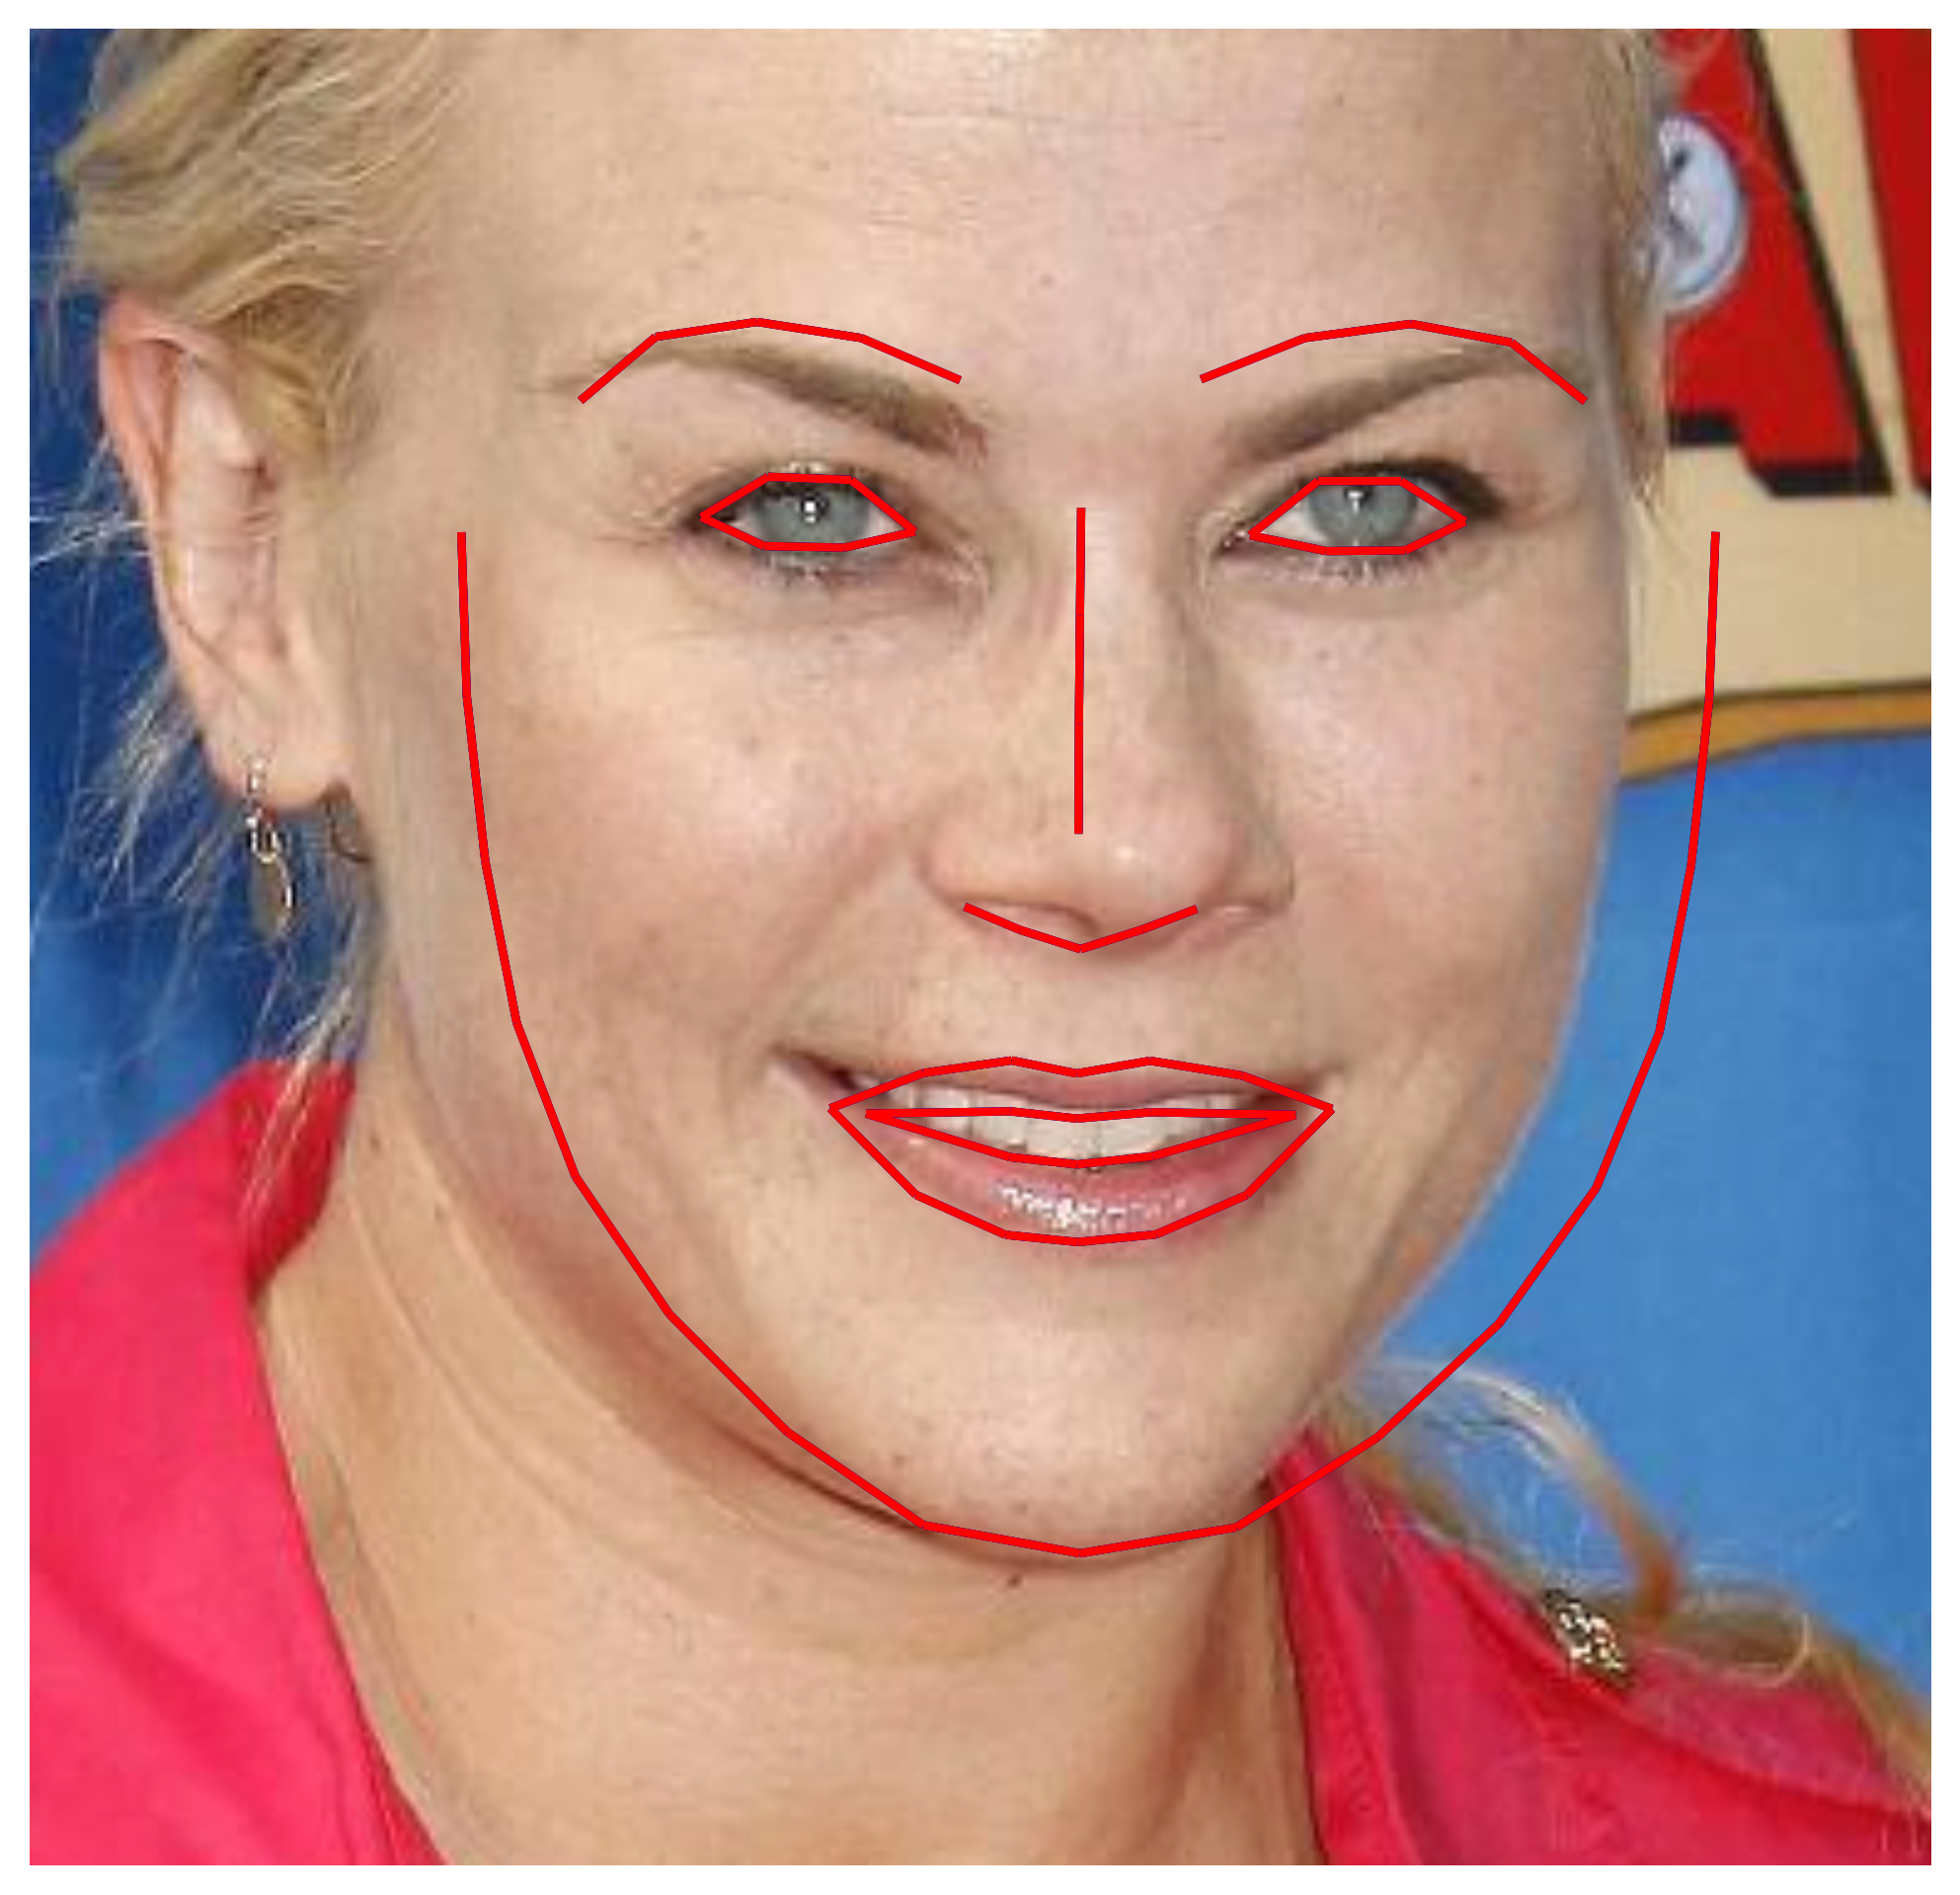
\includegraphics[width=\textwidth]{figures/ini_0.png}
		\caption{$0\%$}
		\label{fig:ini_0}
	\end{subfigure}
	\begin{subfigure}{0.16\textwidth}
		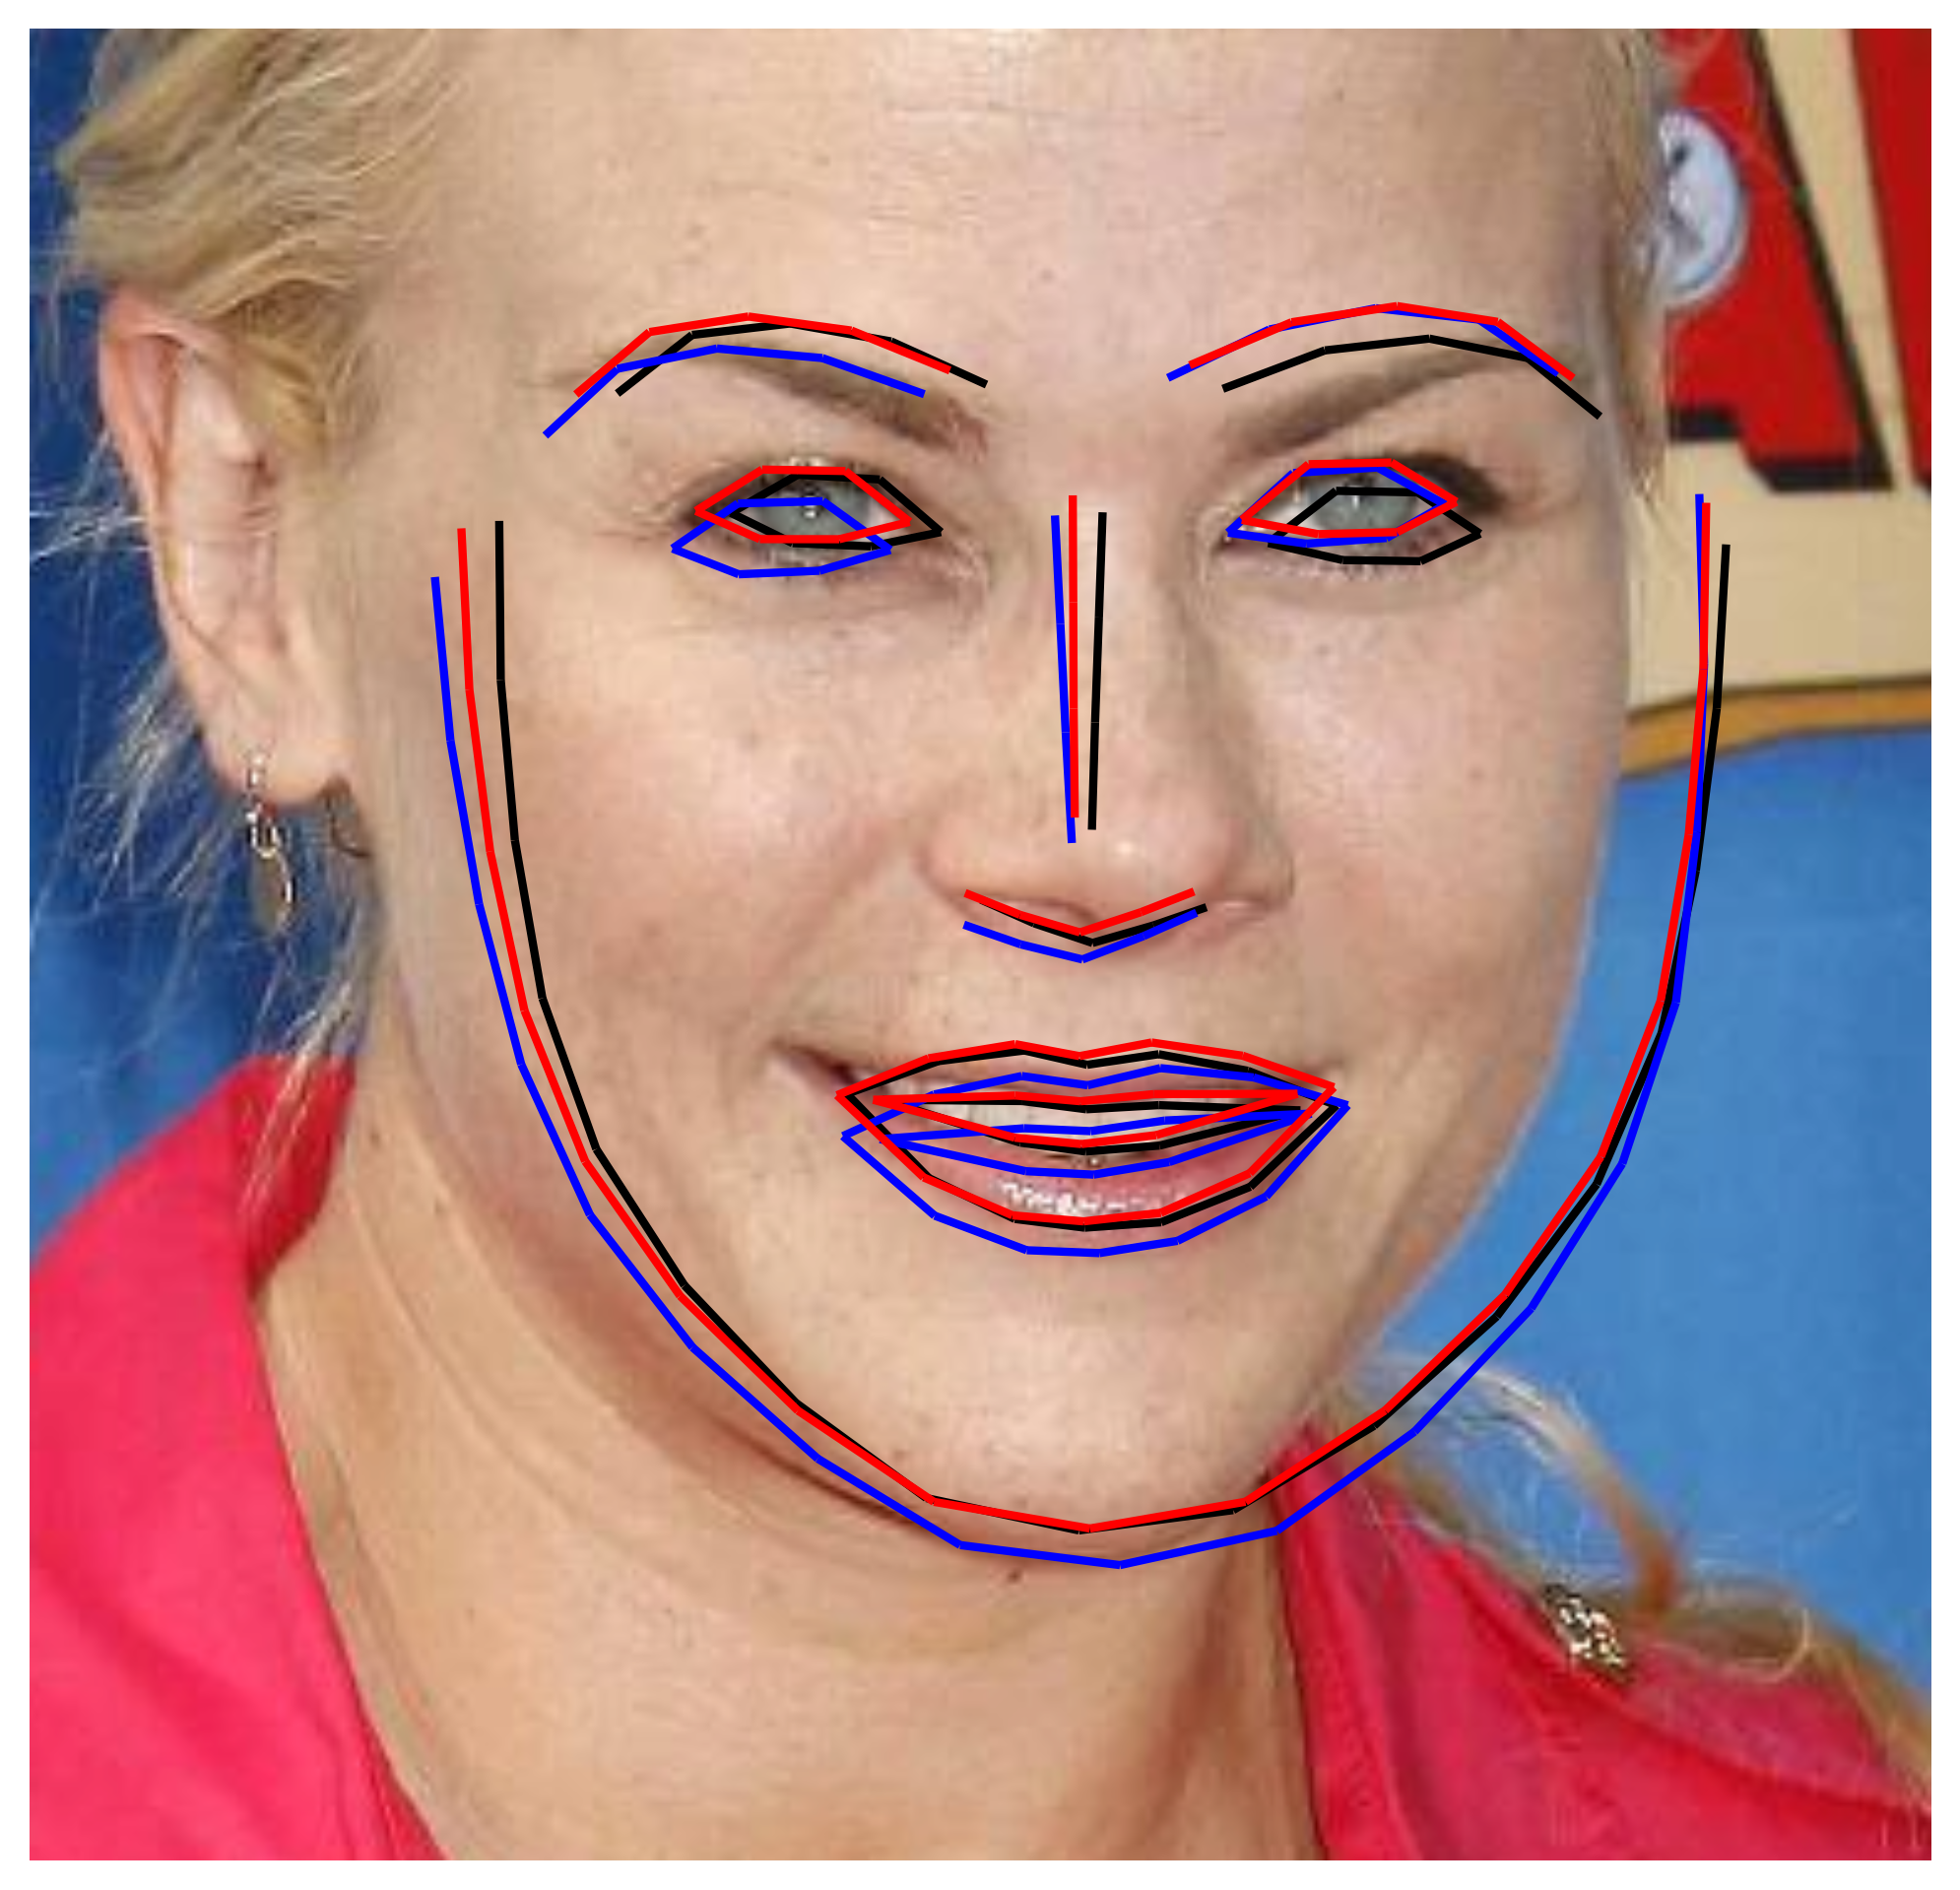
\includegraphics[width=\textwidth]{figures/ini_1.png}
		\caption{$2.5\%$}
		\label{fig:ini_1}
	\end{subfigure}
	\begin{subfigure}{0.16\textwidth}
		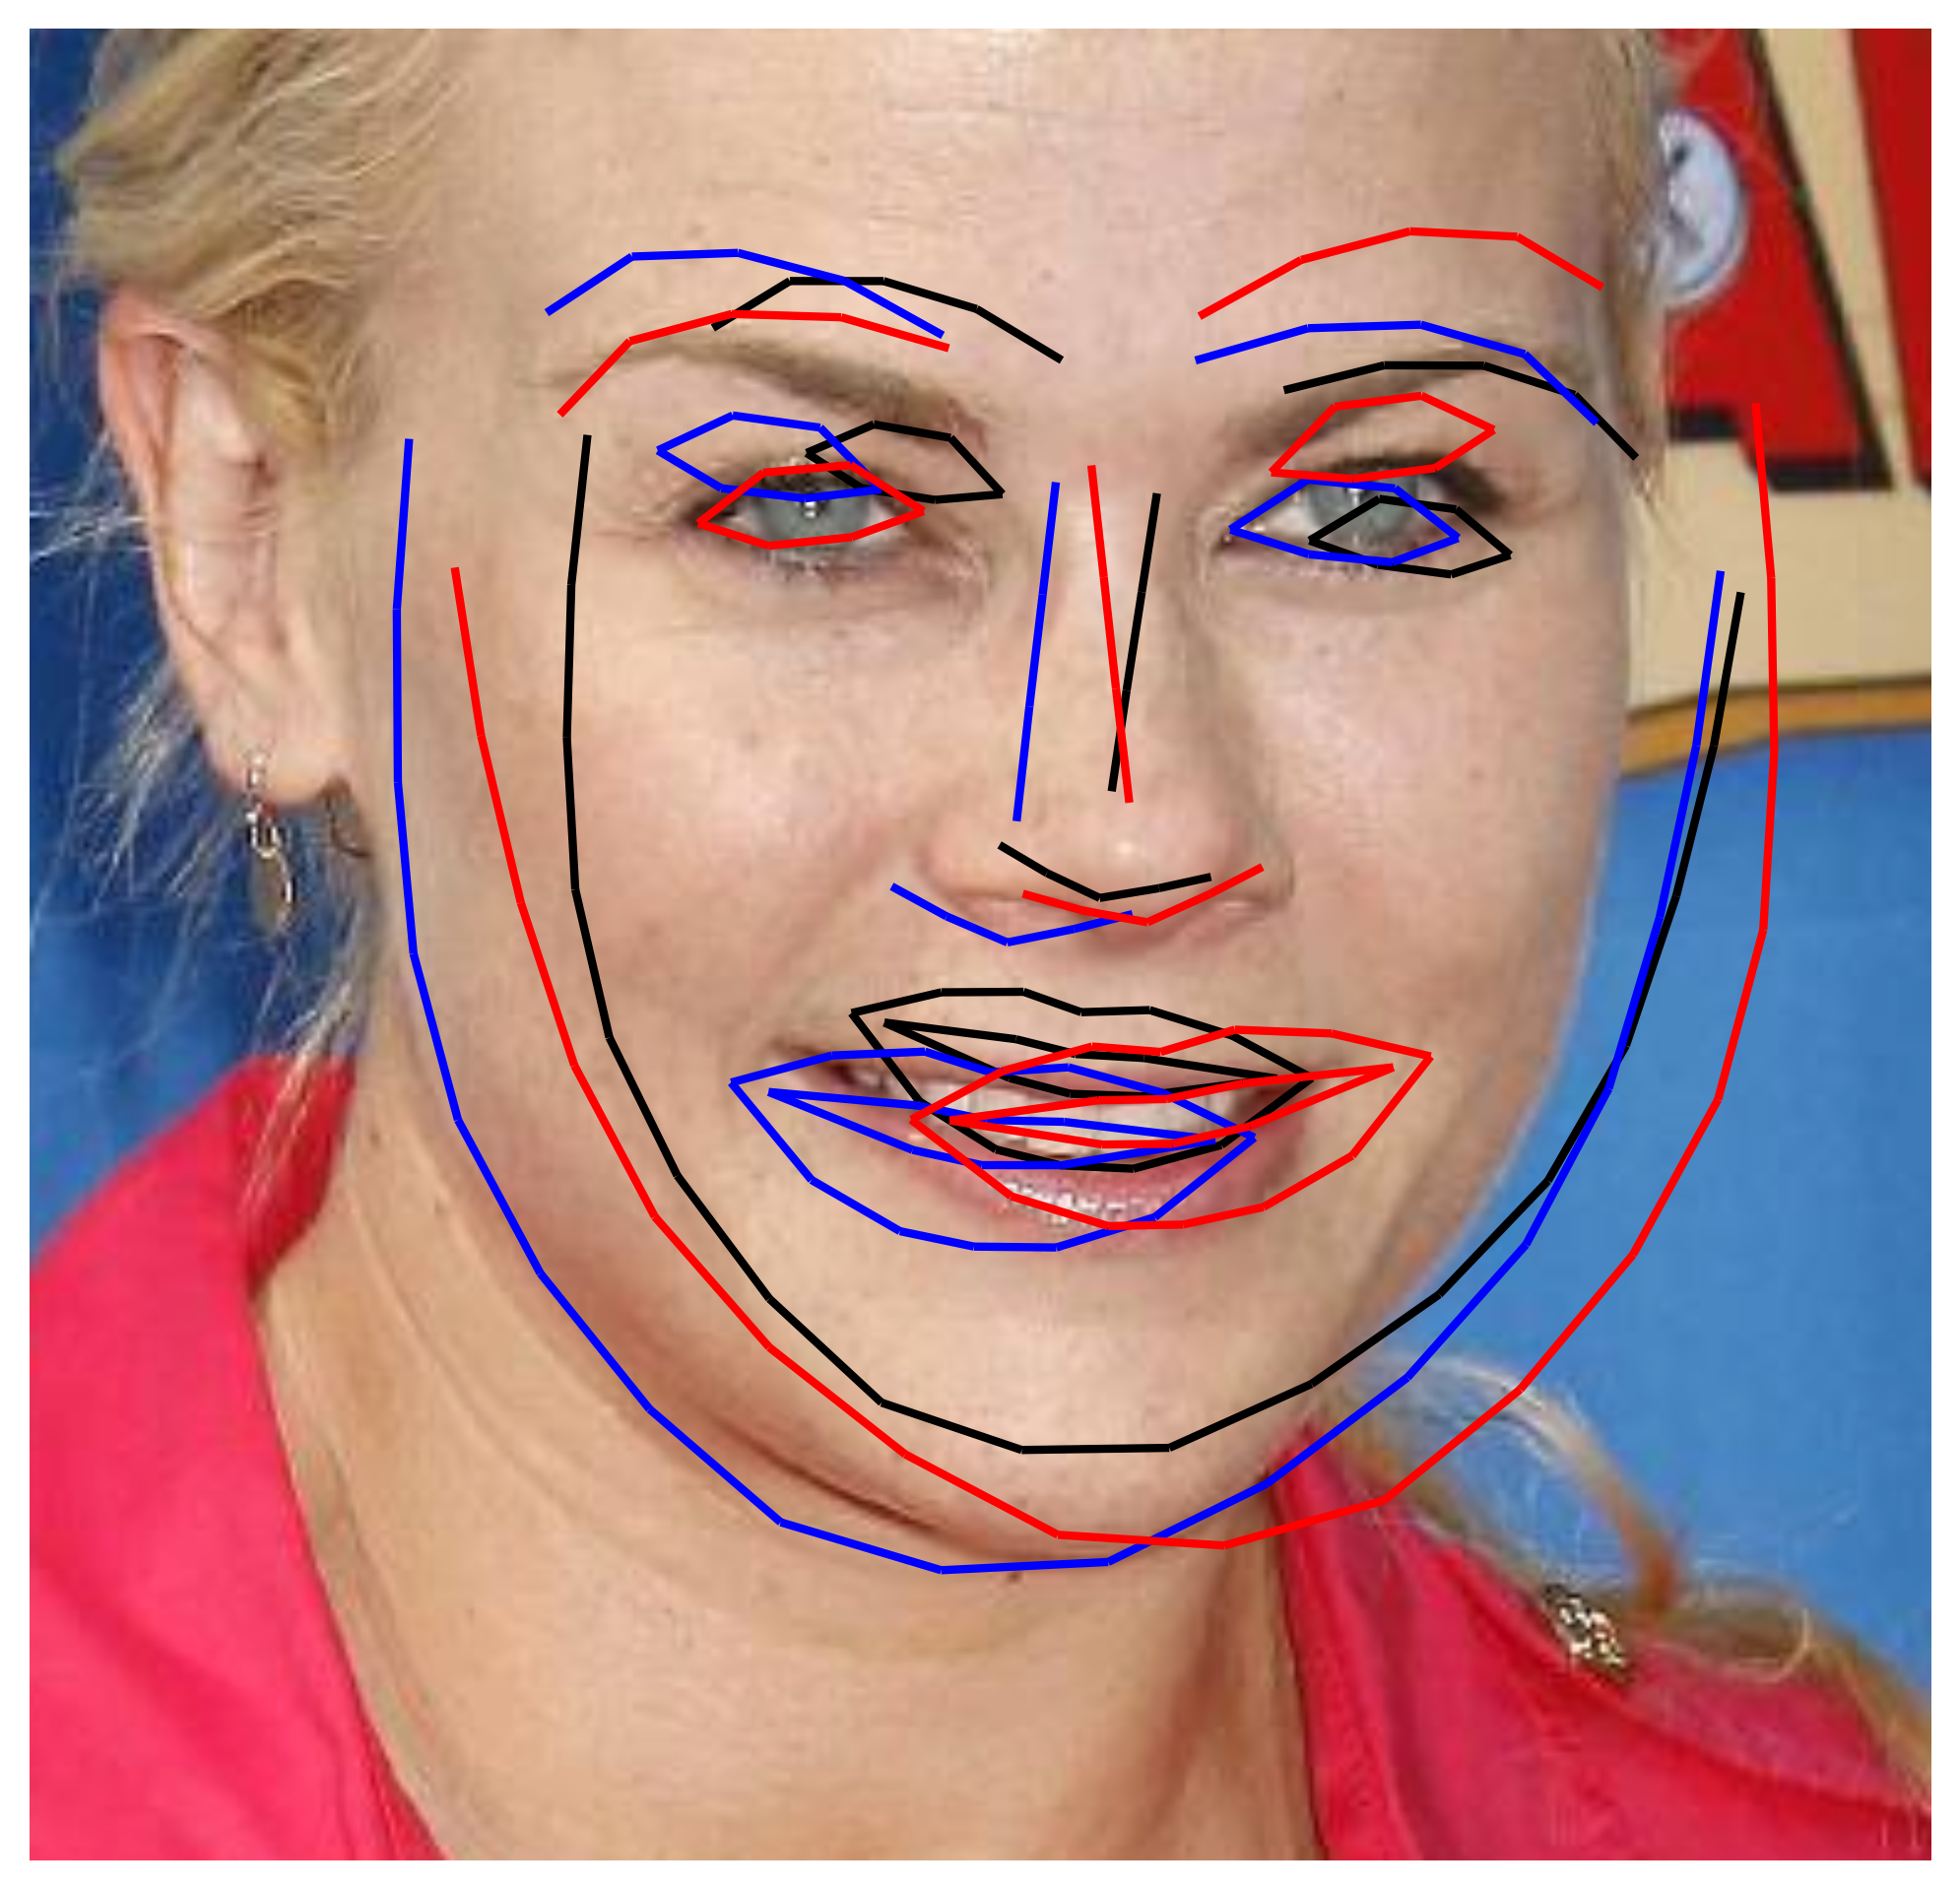
\includegraphics[width=\textwidth]{figures/ini_2.png}
		\caption{$5\%$}
		\label{fig:ini_2}
	\end{subfigure}
	\begin{subfigure}{0.16\textwidth}
		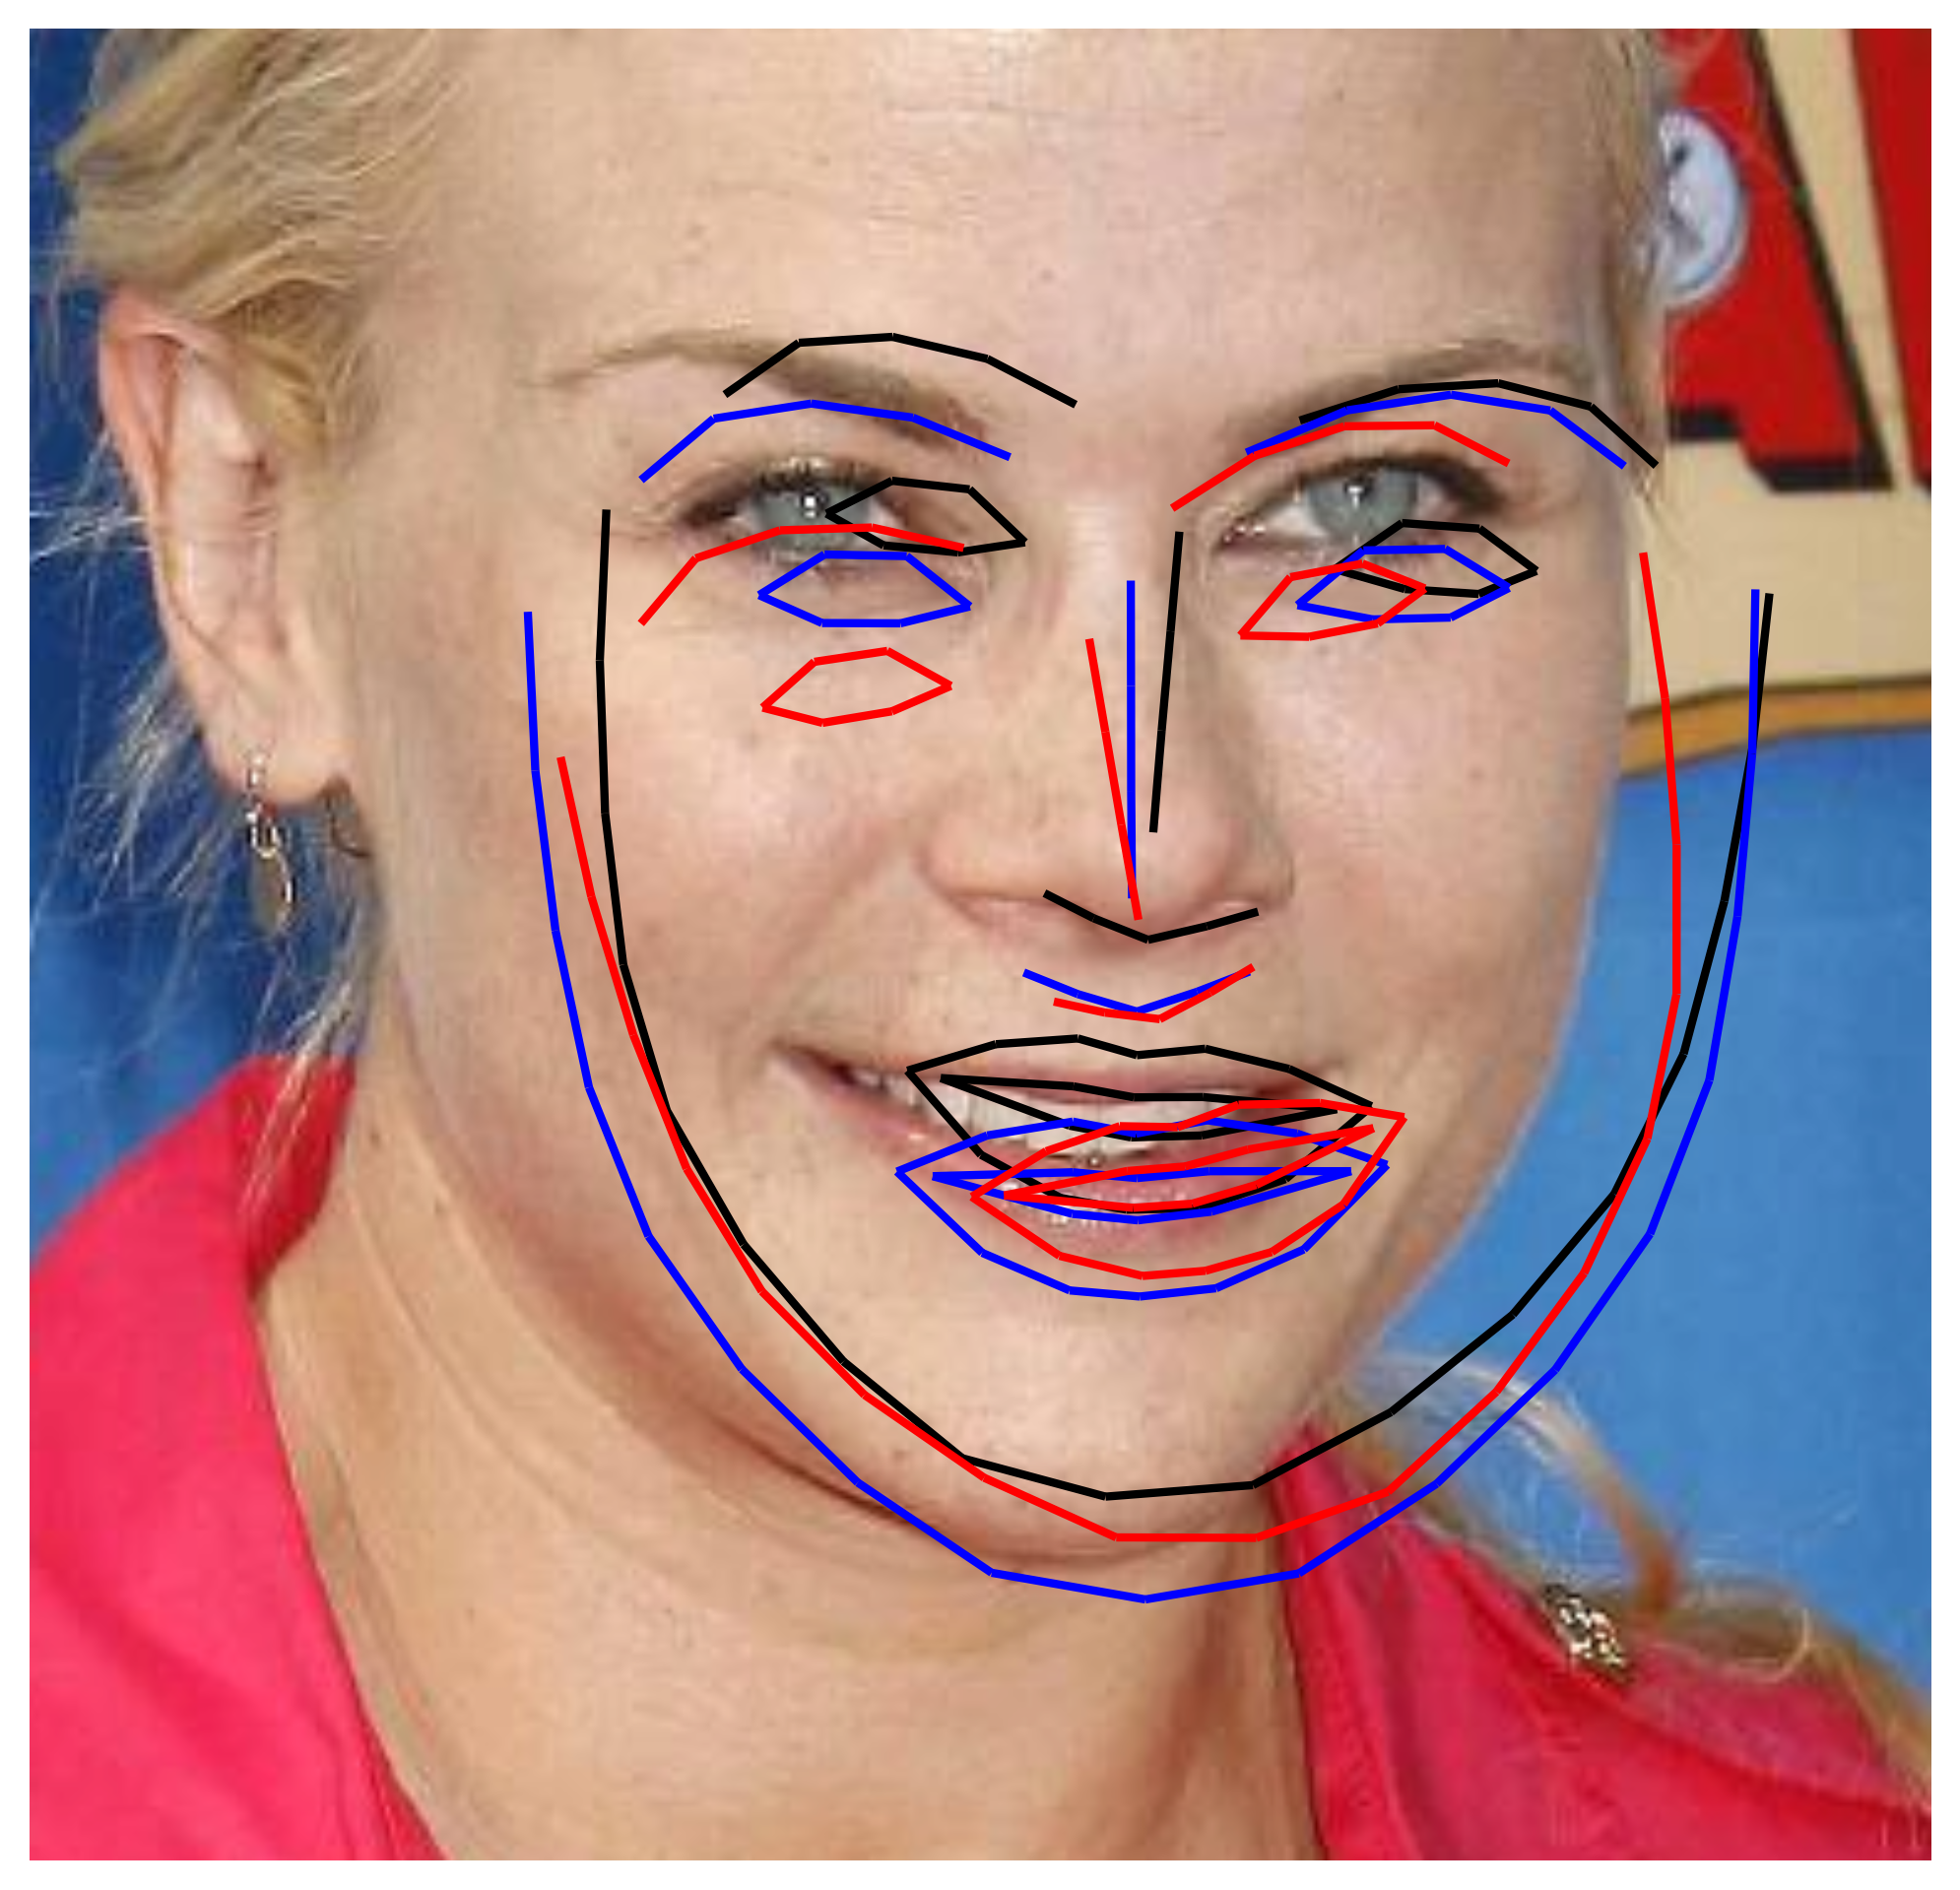
\includegraphics[width=\textwidth]{figures/ini_3.png}
		\caption{$7.5\%$}
		\label{fig:ini_3}
	\end{subfigure}
	\begin{subfigure}{0.16\textwidth}
		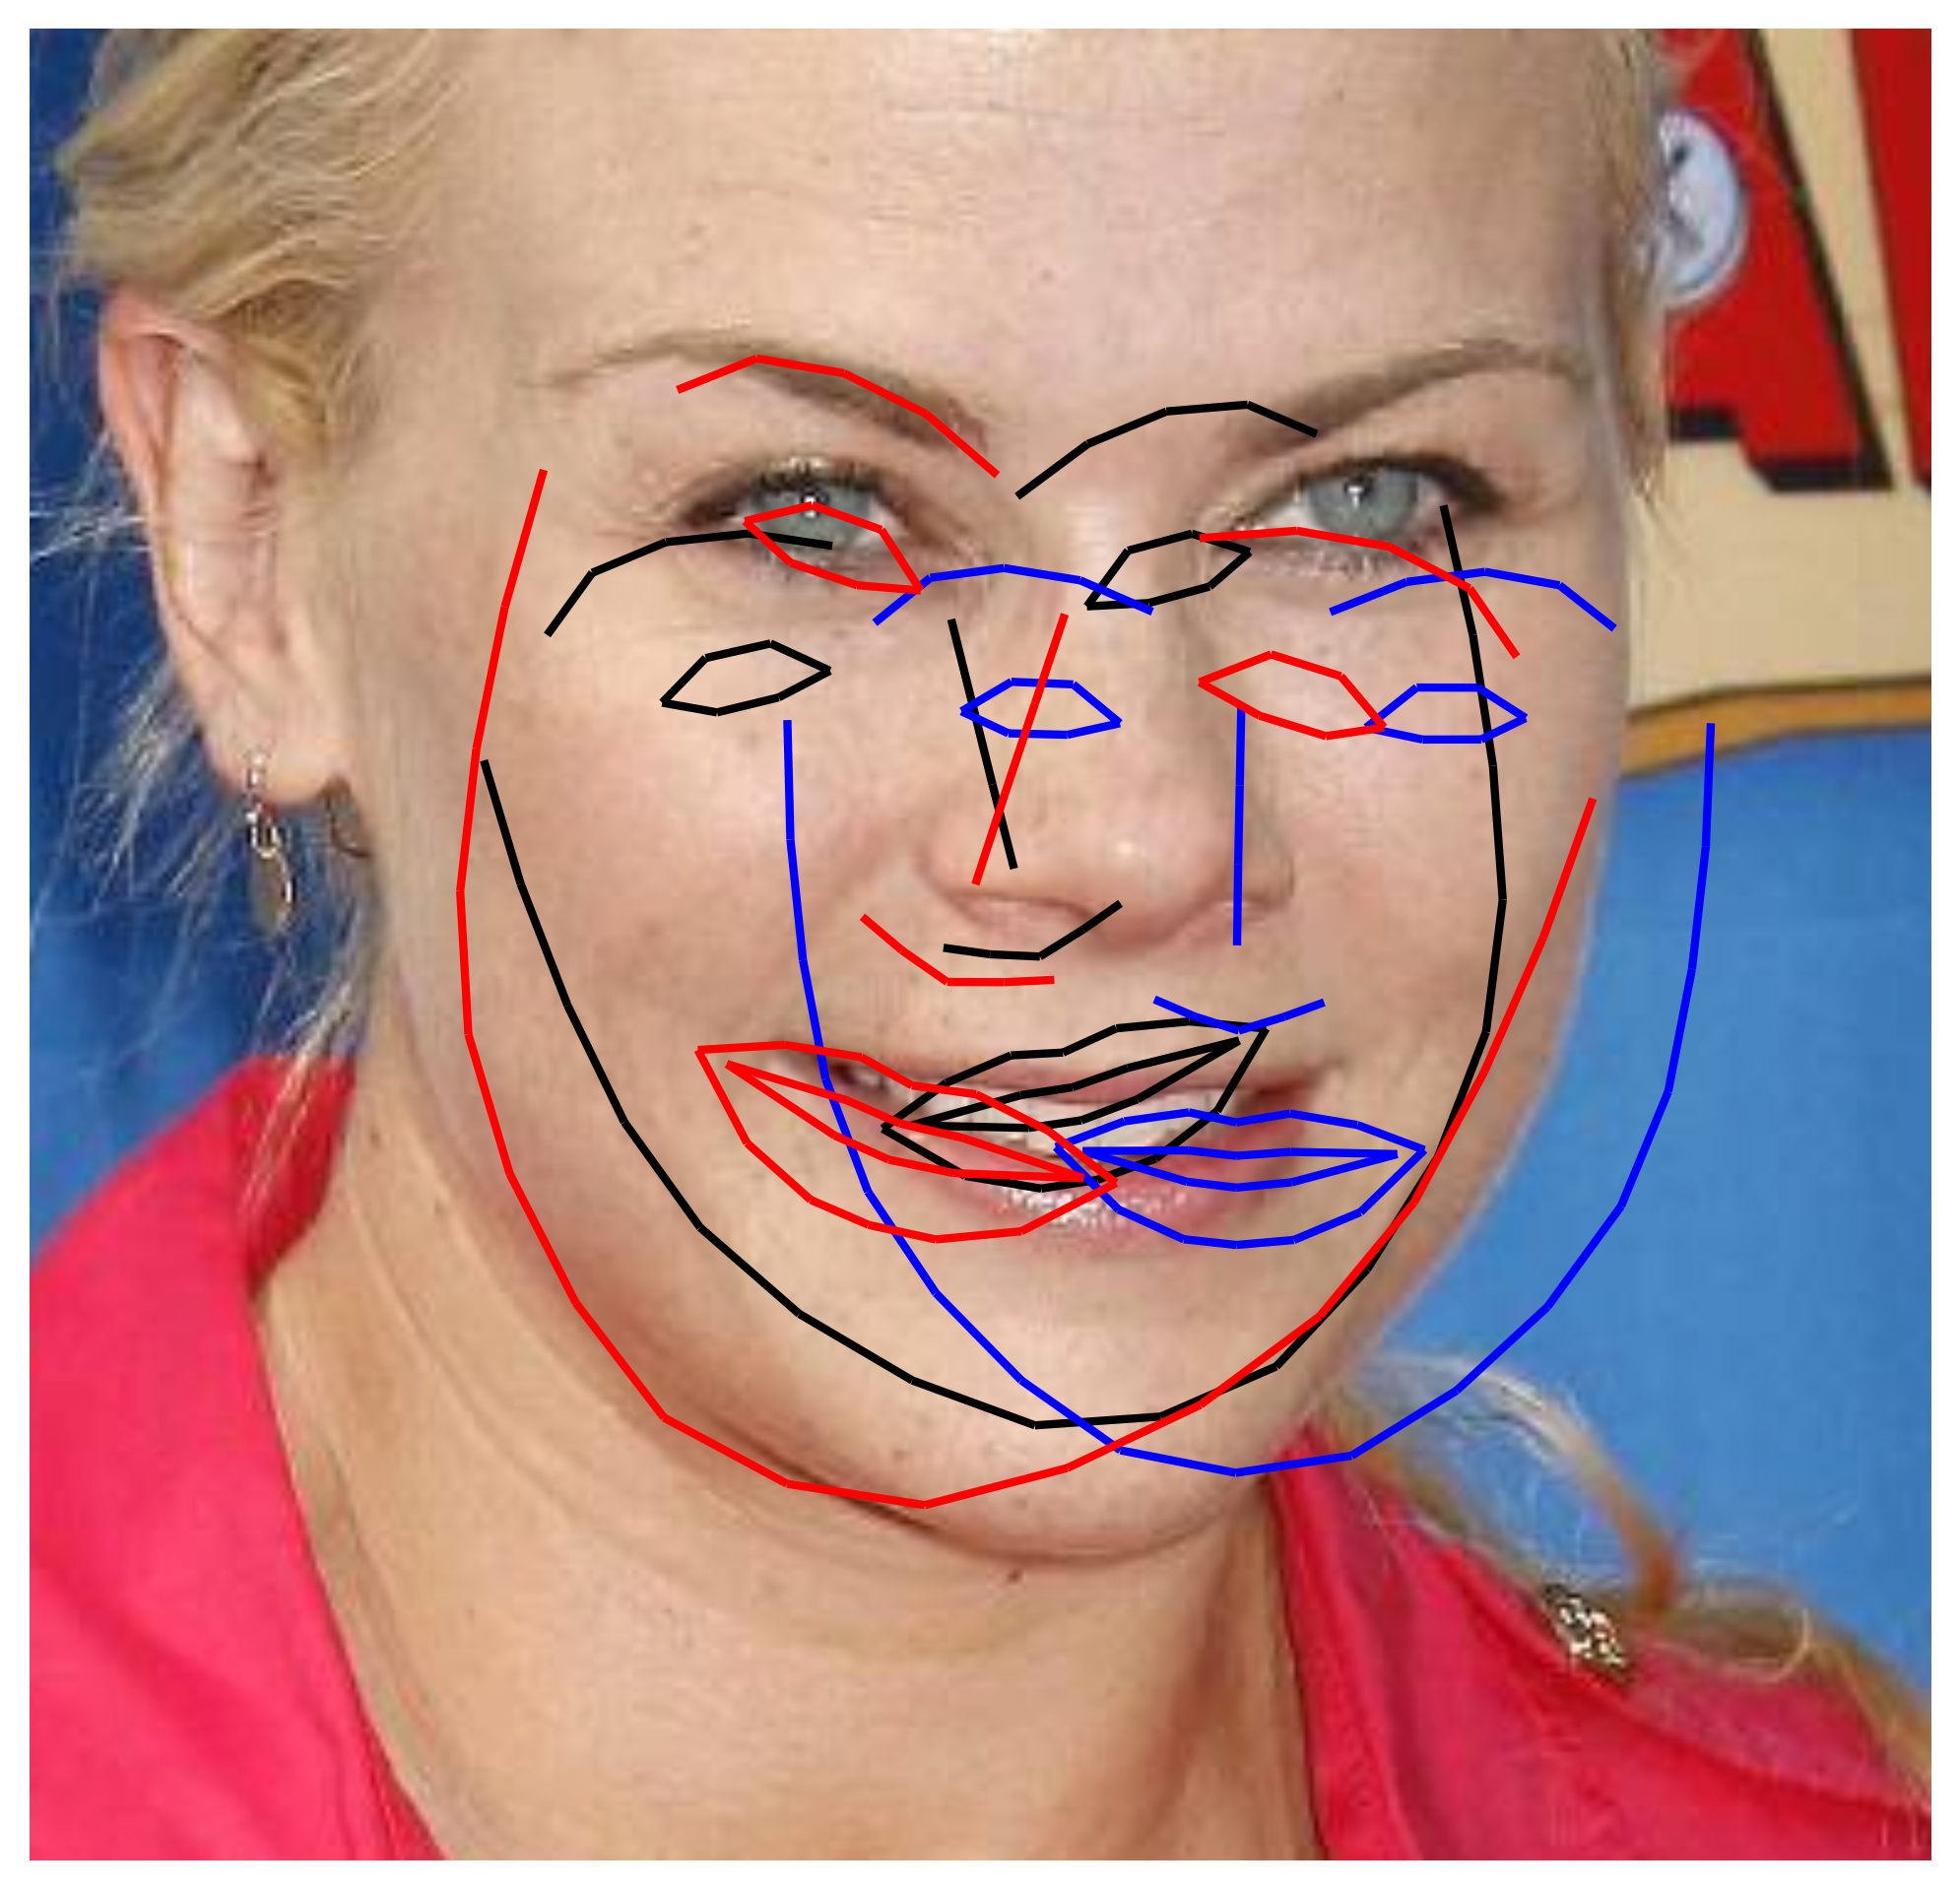
\includegraphics[width=\textwidth]{figures/ini_4.png}
		\caption{$10\%$}
		\label{fig:ini_4}
	\end{subfigure}
    \caption{Exemplar initializations obtained by varying the percentage of uniform noise added to the similarity parameters. Note that, increasing the percentage of noise produces more challenging initialization.}
    \label{fig:ini}
\end{figure*}

In this section we analyze the performance of all CGD algorithms derived in Section \ref{sec:fitting} on the specific problem of non-rigid face alignment in-the-wild. We start by quantifying the fitting accuracy and convergence properties of each algorithm.

We use a single AAM, built with $\sim800$ training images of the Labeled Face Parts in the Wild (LFPW) \cite{Belhumeur2011} and $\sim2000$ Helen \cite{Le2012} databases, to test all algorithms. Similar to \cite{Tzimiropoulos2014}, a modified version of the \emph{Dense} Scale Invariant Feature Transform (DSIFT) \cite{Lowe1999, Dalal2005} is used to define the appearance representation of the previous AAM. In particular, we describe each pixel with a reduced SIFT descriptor of length $8$ using the public implementation provided by the authors of \cite{Vedaldi2008vlfeat}. All algorithms are implemented in a coarse to fine manner using a Gaussian pyramid with $2$ levels (face images are normalized to a \emph{face size}\footnote{We use the definition of face size given in \cite{Zhu2012} i.e. computed as the mean of the face height and width.} of roughly $150$ pixels at the top level). In all experiments, we optimized over $7$ shape parameters ($4$ similarity transform and $3$ non-rigid shape parameters) at the first pyramid level and over $16$ shape parameters ($4$ similarity transform and $12$ non-rigid shape parameters) at the second one. The dimensionality of the appearance models is kept to represent $75\%$ of the total variance in both levels. This results in $225$ and $280$ appearance parameters at the first and second pyramid levels respectively. The previous choices were determined by testing on a small hold out set of the training data. 

In all experiments, algorithms are initialized by perturbing the similarity transforms that perfectly align the model's mean shape (a frontal pose and neutral expression looking shape) with the ground truth shape of each image. These transforms are perturbed by adding uniformly distributed random noise to their scale, rotation and translation parameters. Exemplar initializations obtained by this procedure for different percentages of uniform noise are shown in Figure \ref{fig:ini}.

Finally, in order to encourage open research and facilitate future comparisons with the results presented in this section, we make the implementation of all CGD algorithms publicly available as part of the Menpo Project \cite{Menpo2014}.

\subsection{Comparison on LFPW}

In this experiment, we report the fitting accuracy and convergence properties of each of the previous algorithms. In order to keep the information on each figure and table easily readible and interpretable the experiment by grouping al...


\subsubsection{SSD algorithms}


\subsubsection*{Gauss-Newton}

\begin{figure*}[h!]
	\centering
	\begin{subfigure}{0.48\textwidth}
	    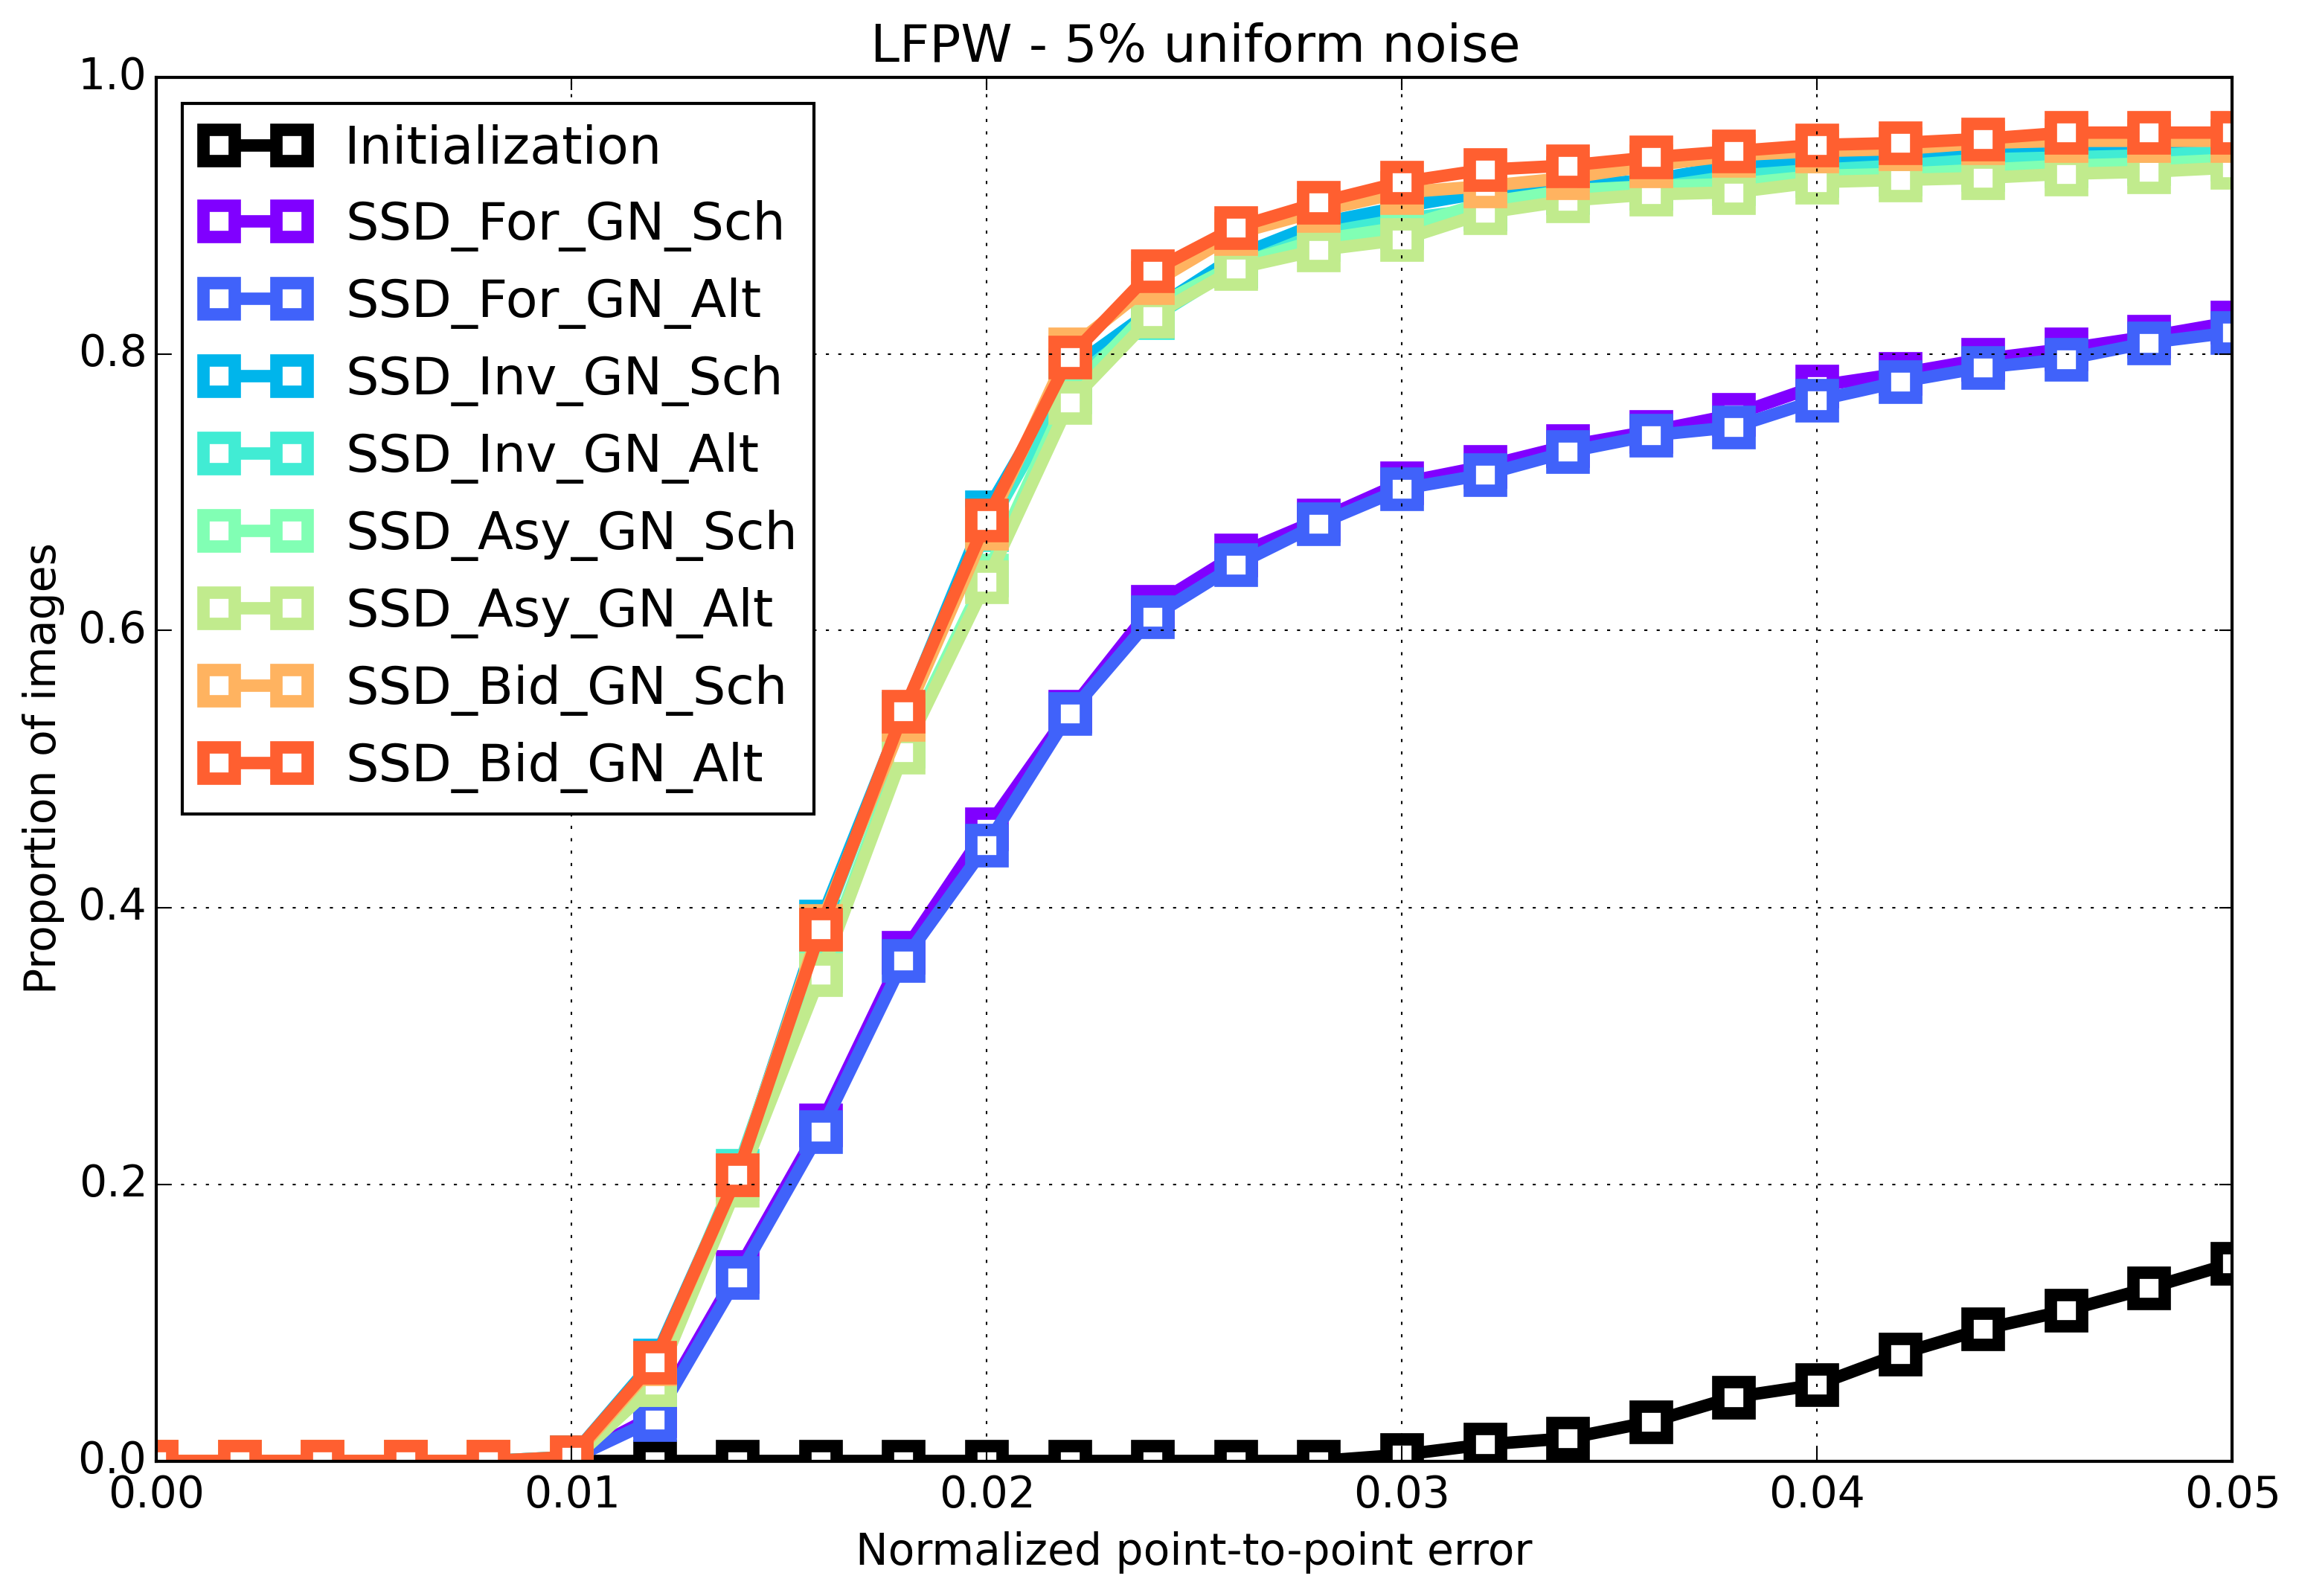
\includegraphics[width=\textwidth]{experiments/algorithms/ssd_gn/ced_ssd_gn_5.png}
	    \caption{Cumulative Error Distribution graph on the LFPW test dataset for all SSD Gauss-Newton algorithms initialized with $5\%$ uniform noise.}
	    \label{fig:ced_ssd_gn_5}
	\end{subfigure}
	\hfill
	\begin{subfigure}{0.48\textwidth}
	    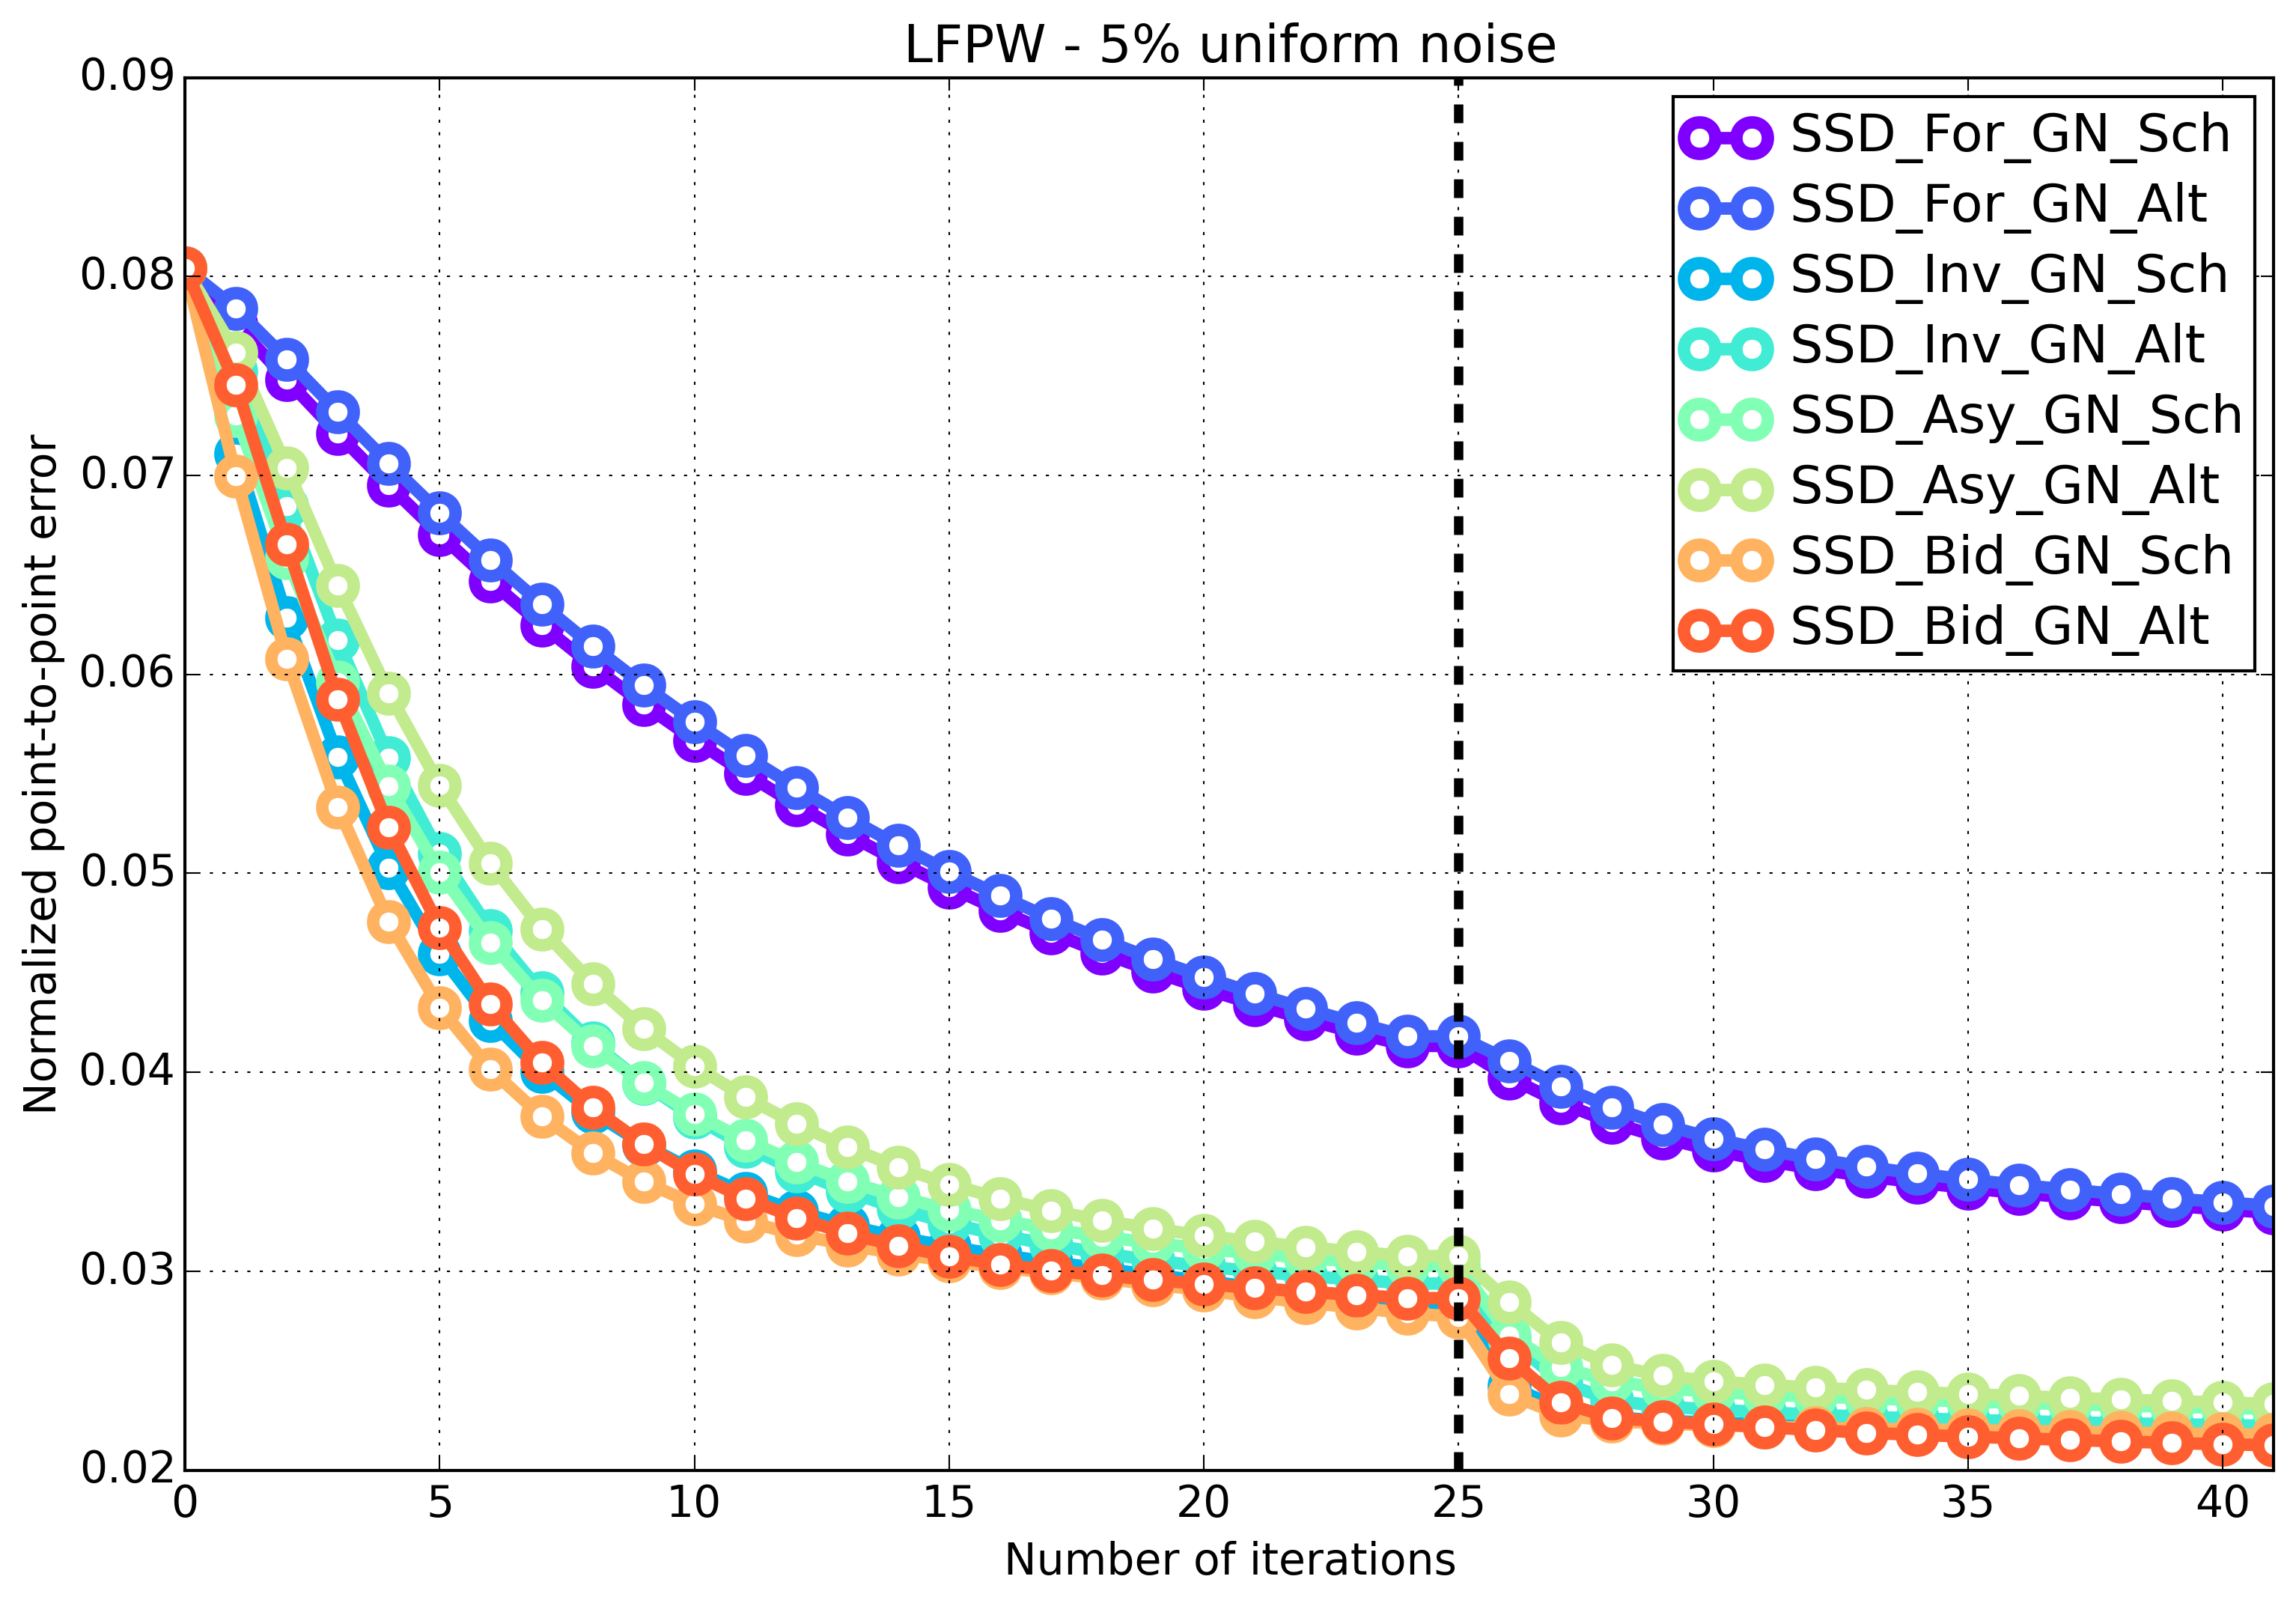
\includegraphics[width=\textwidth]{experiments/algorithms/ssd_gn/mean_error_vs_iters_ssd_gn_5.png}
	    \caption{Mean normalized point-to-point error vs number of iterations graph on the LFPW test dataset for all SSD Gauss-Newton algorithms initialized with $5\%$ uniform noise.}
	    \label{fig:mean_error_vs_iters_ssd_gn_5}
	\end{subfigure}
	\par\medskip
	\begin{subfigure}{0.48\textwidth}
	    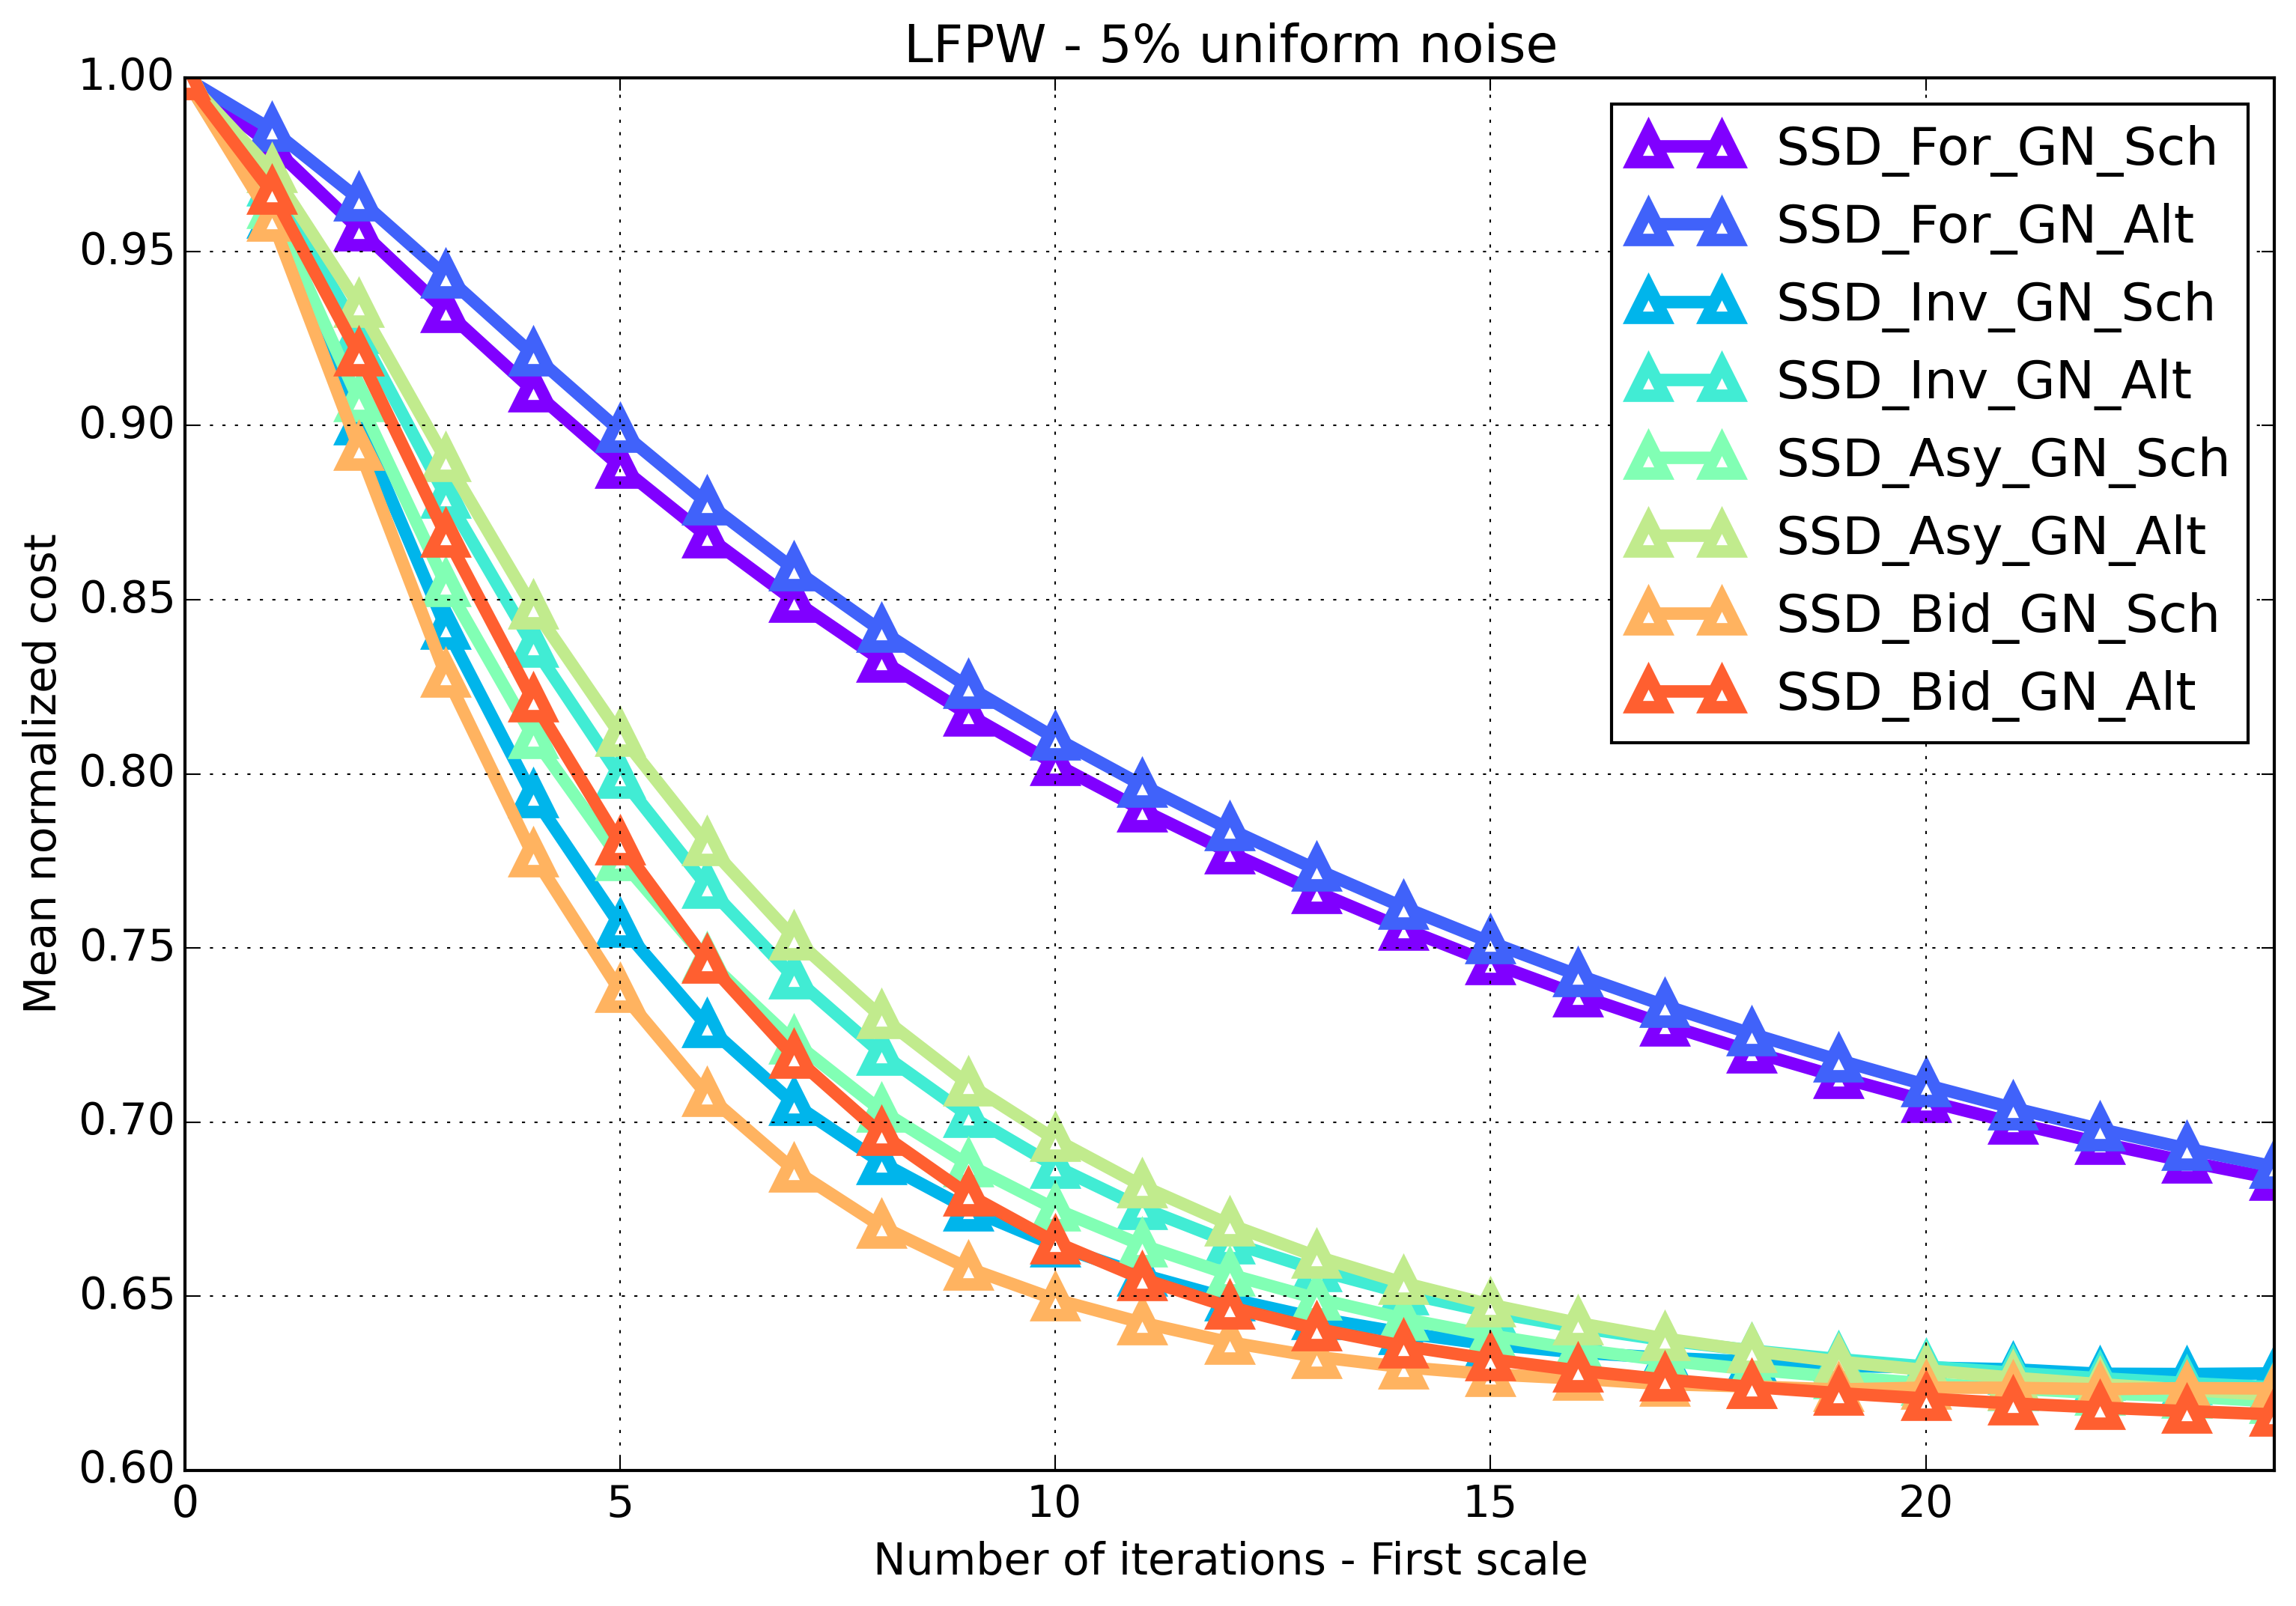
\includegraphics[width=\textwidth]{experiments/algorithms/ssd_gn/mean_cost_vs_iters1_ssd_gn_5.png}
	    \caption{Mean normalized cost vs number of first scale iterations graph on the LFPW test dataset for all SSD Gauss-Newton algorithms initialized with $5\%$ uniform noise.}
	    \label{fig:mean_cost_vs_iters1_ssd_gn_5}
	\end{subfigure}
	\hfill
	\begin{subfigure}{0.48\textwidth}
	    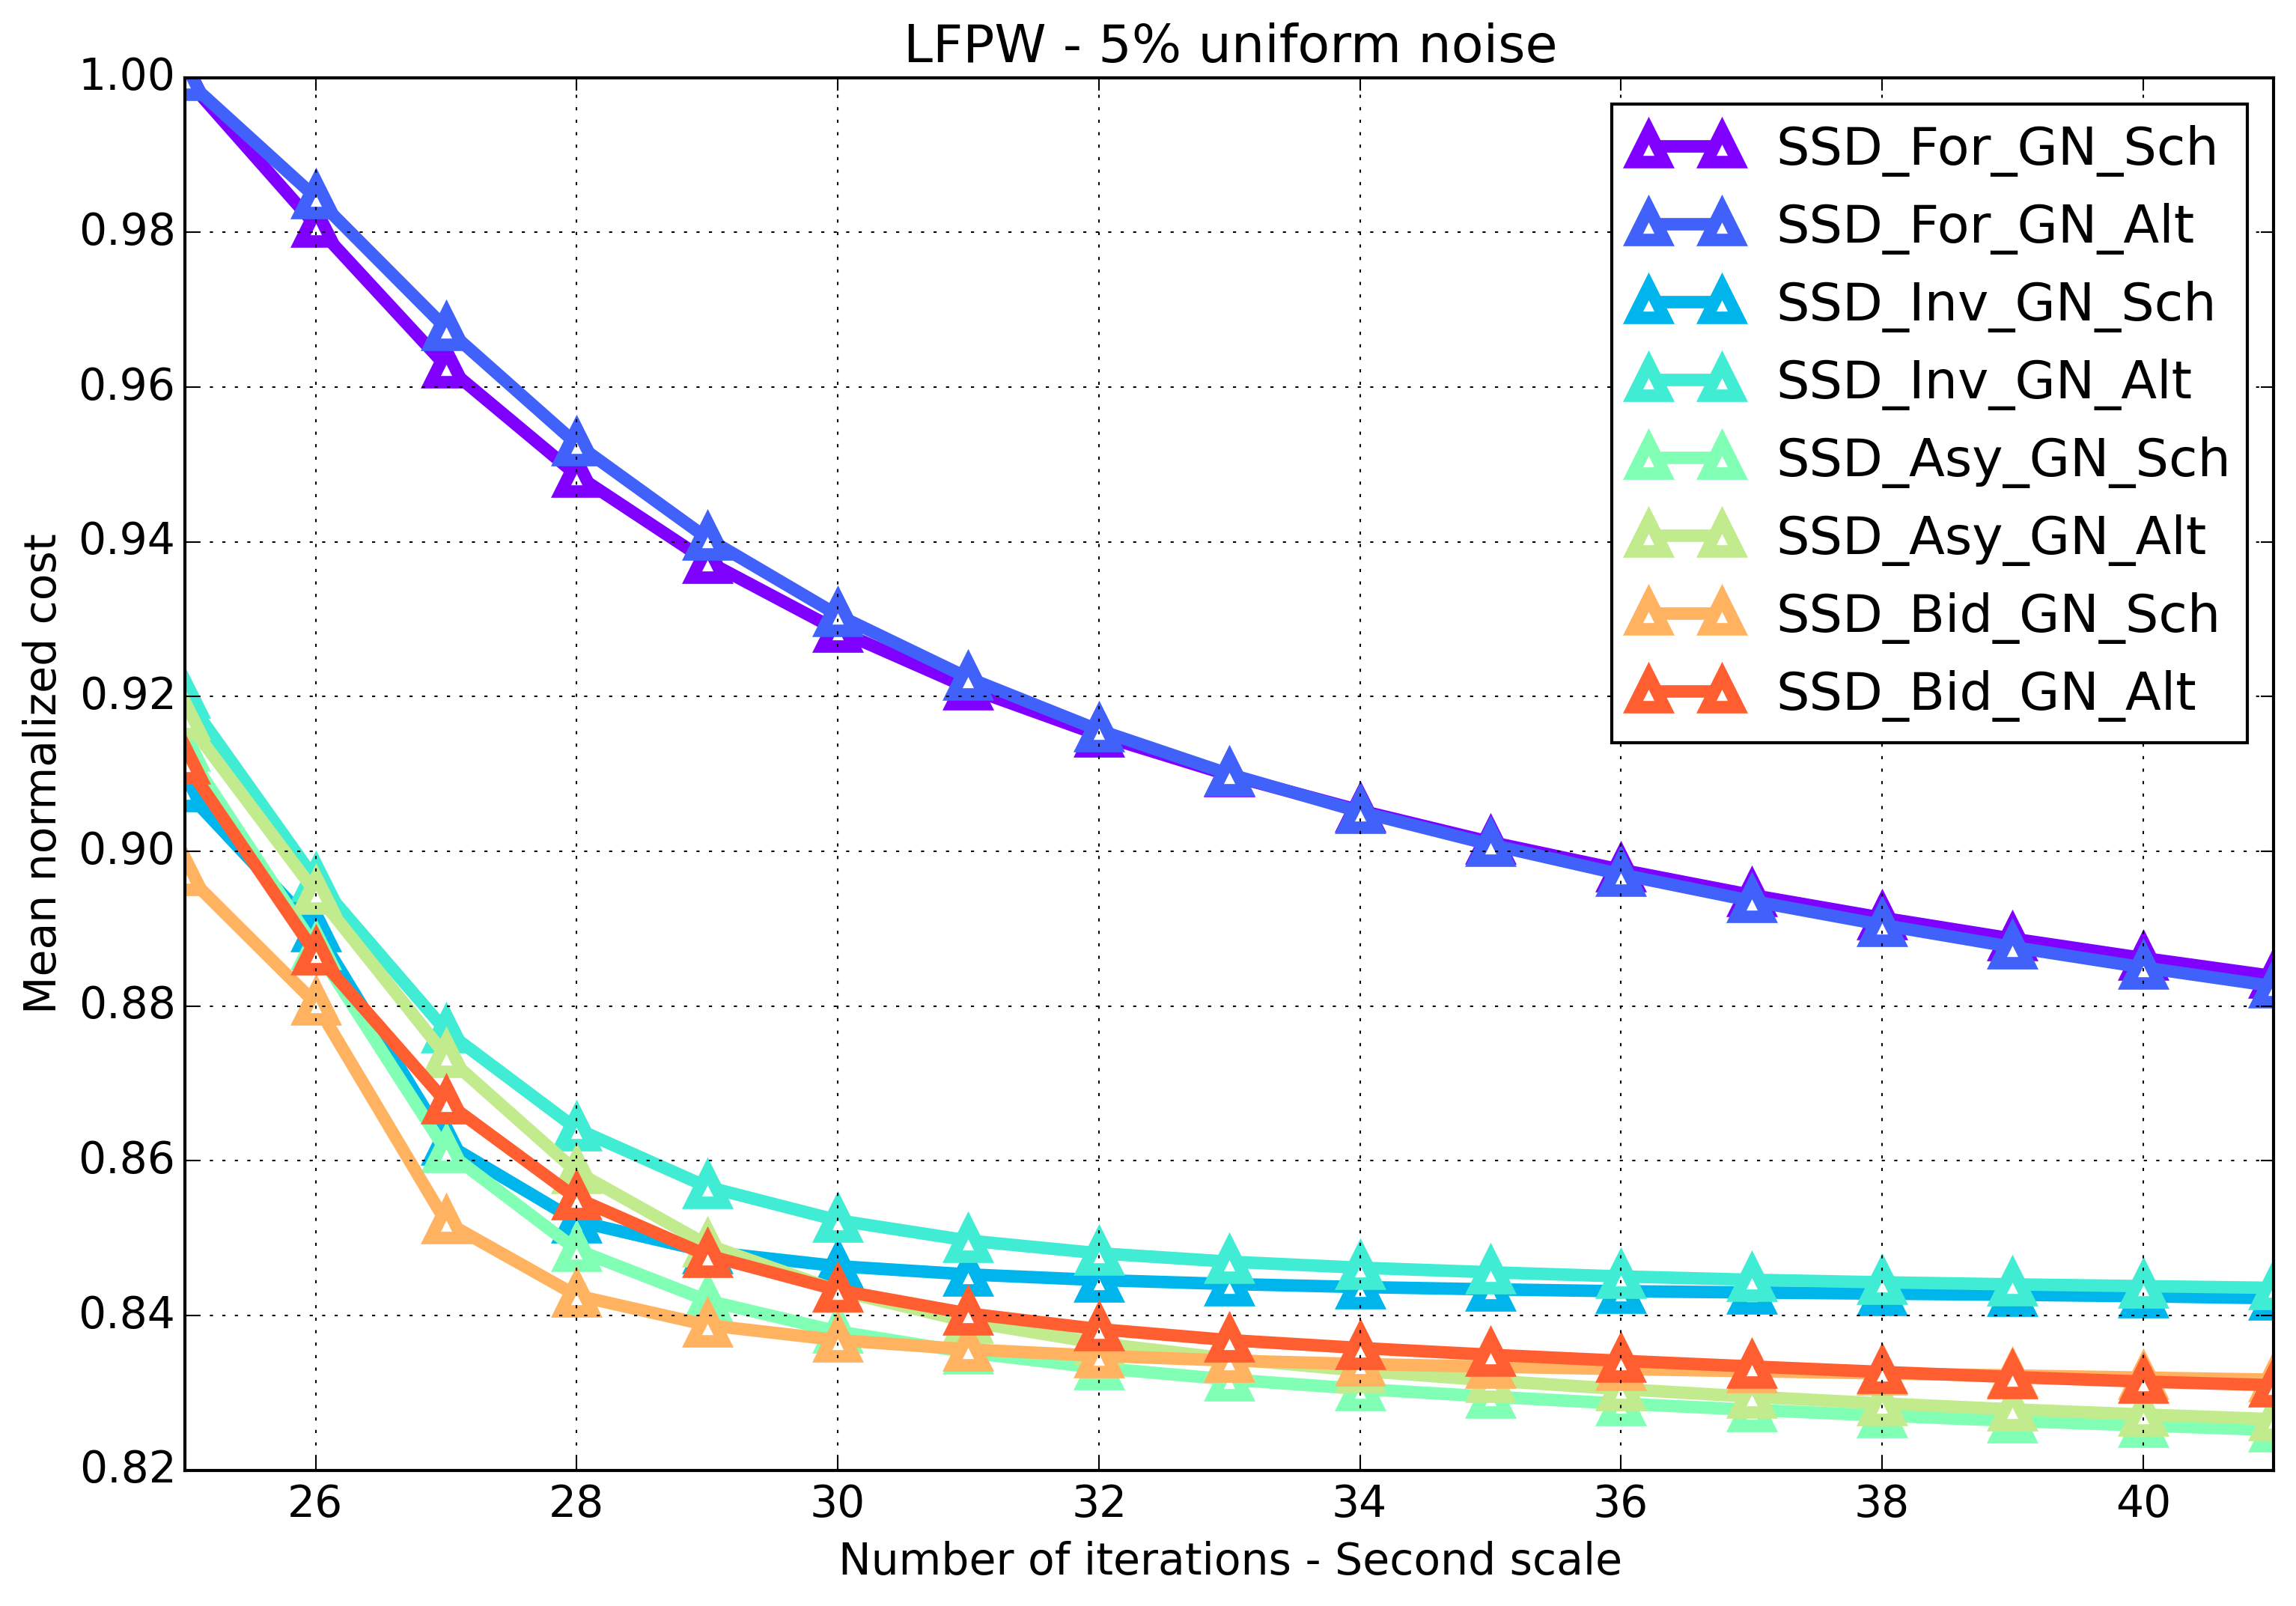
\includegraphics[width=\textwidth]{experiments/algorithms/ssd_gn/mean_cost_vs_iters2_ssd_gn_5.png}
	    \caption{Mean normalized cost vs number of second scale iterations graph on the LFPW test dataset for all SSD Gauss-Newton algorithms initialized with $5\%$ uniform noise.}
	    \label{fig:mean_cost_vs_iters2_ssd_gn_5}
	\end{subfigure}
	\label{fig:ssd_gn_5}
	\caption{}
\end{figure*}


\subsubsection*{Wiberg}

\begin{figure*}[h!]
	\centering
	\begin{subfigure}{0.48\textwidth}
	    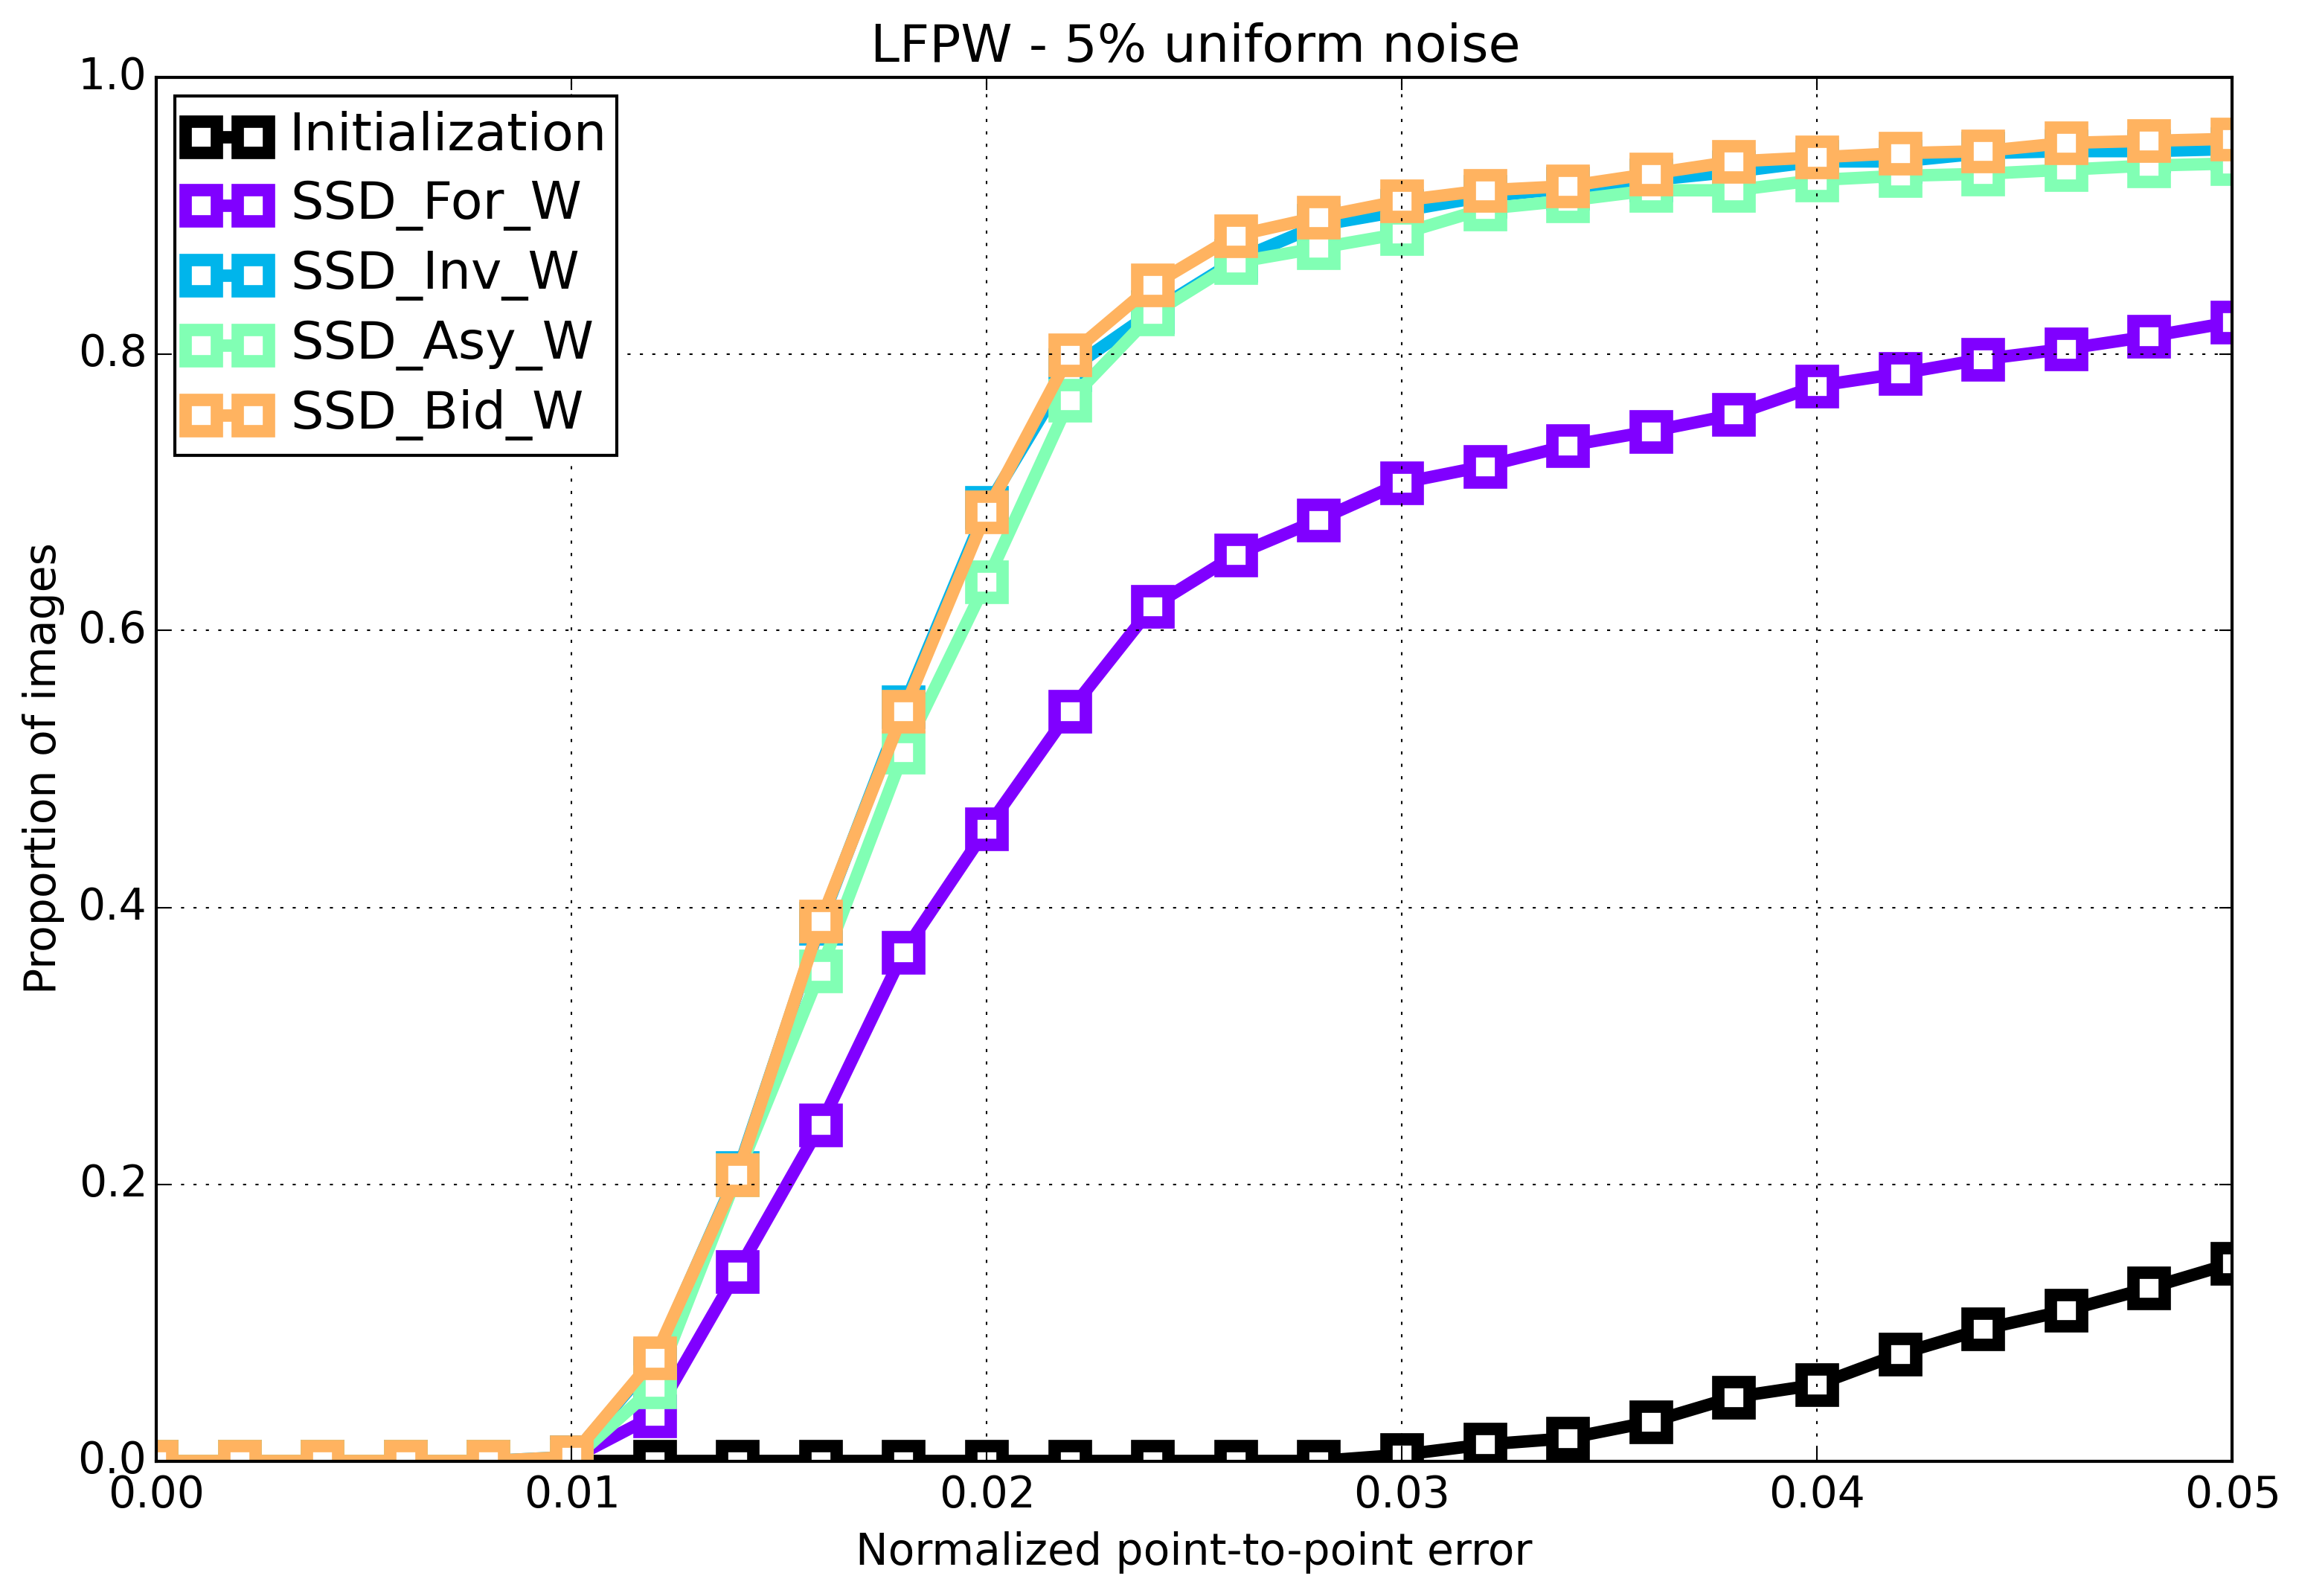
\includegraphics[width=\textwidth]{experiments/algorithms/ssd_w/ced_ssd_w_5.png}
	    \caption{Cumulative Error Distribution graph on the LFPW test dataset for all SSD Wiberg algorithms initialized with $5\%$ uniform noise.}
	    \label{fig:ced_ssd_w_5}
	\end{subfigure}
	\hfill
	\begin{subfigure}{0.48\textwidth}
	    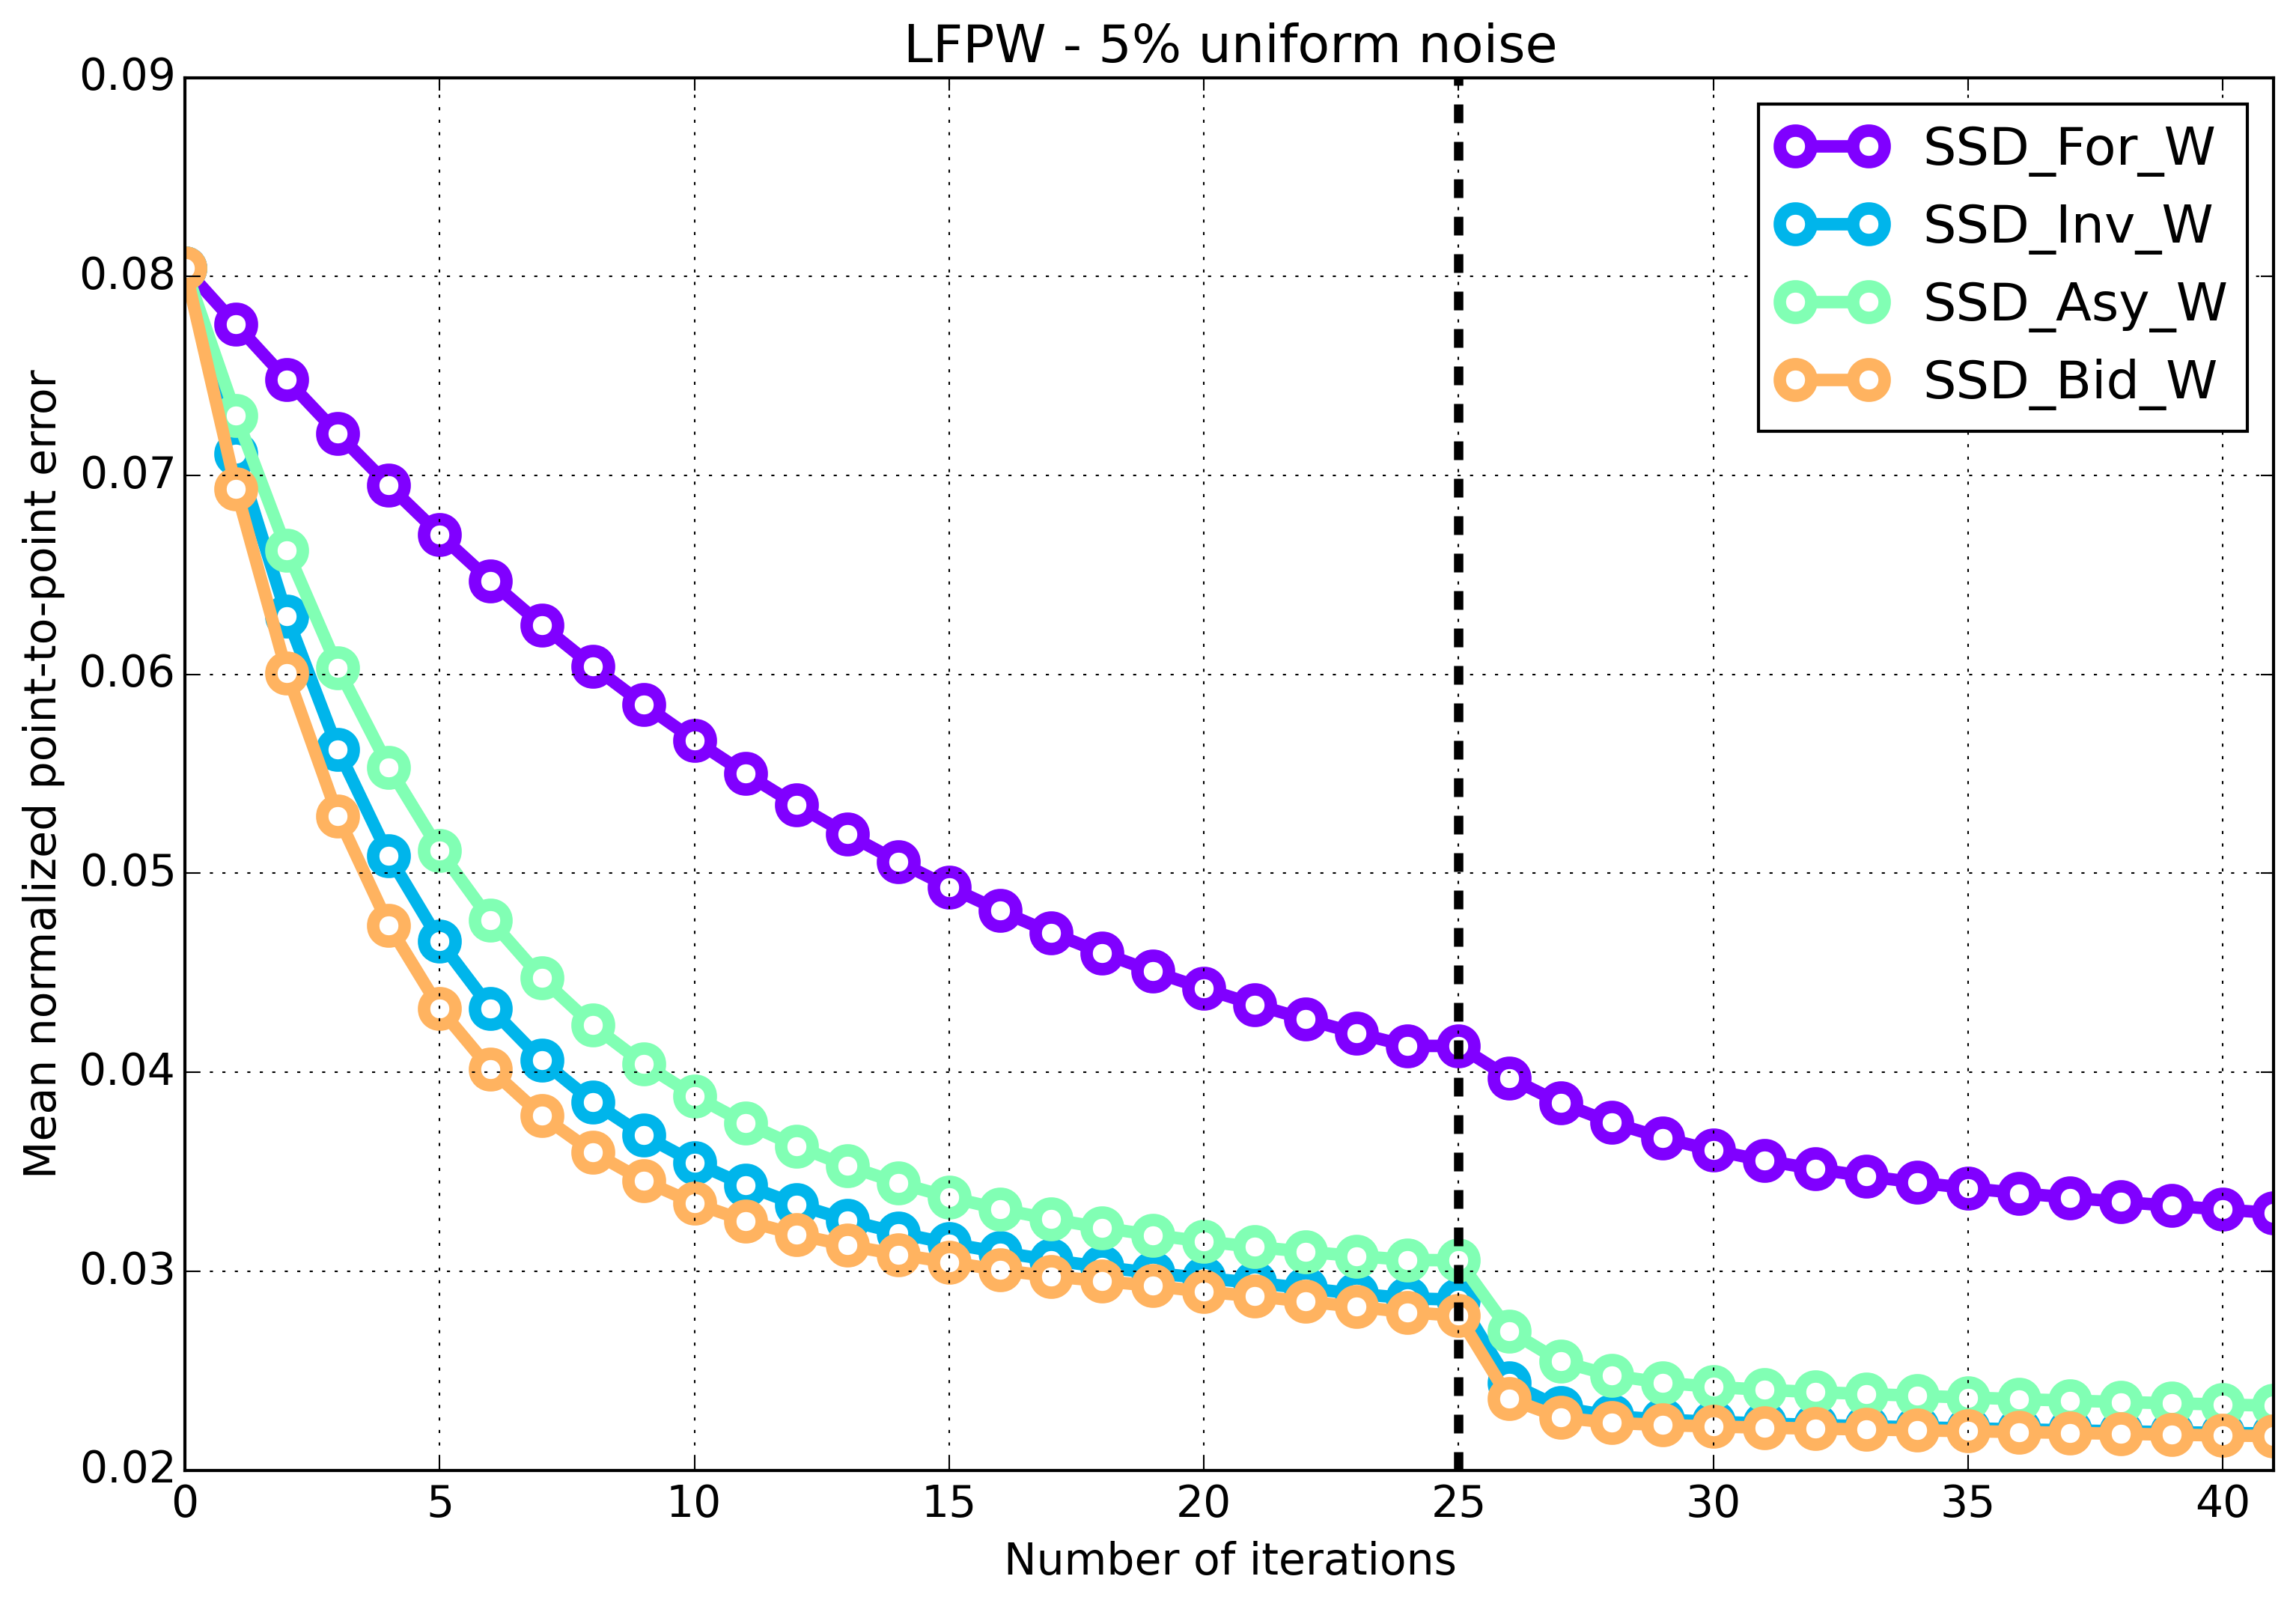
\includegraphics[width=\textwidth]{experiments/algorithms/ssd_w/mean_error_vs_iters_ssd_w_5.png}
	    \caption{Mean normalized point-to-point error vs number of iterations graph on the LFPW test dataset for all SSD Wiberg algorithms initialized with $5\%$ uniform noise.}
	    \label{fig:mean_error_vs_iters_ssd_w_5}
	\end{subfigure}
	\par\medskip
	\begin{subfigure}{0.48\textwidth}
	    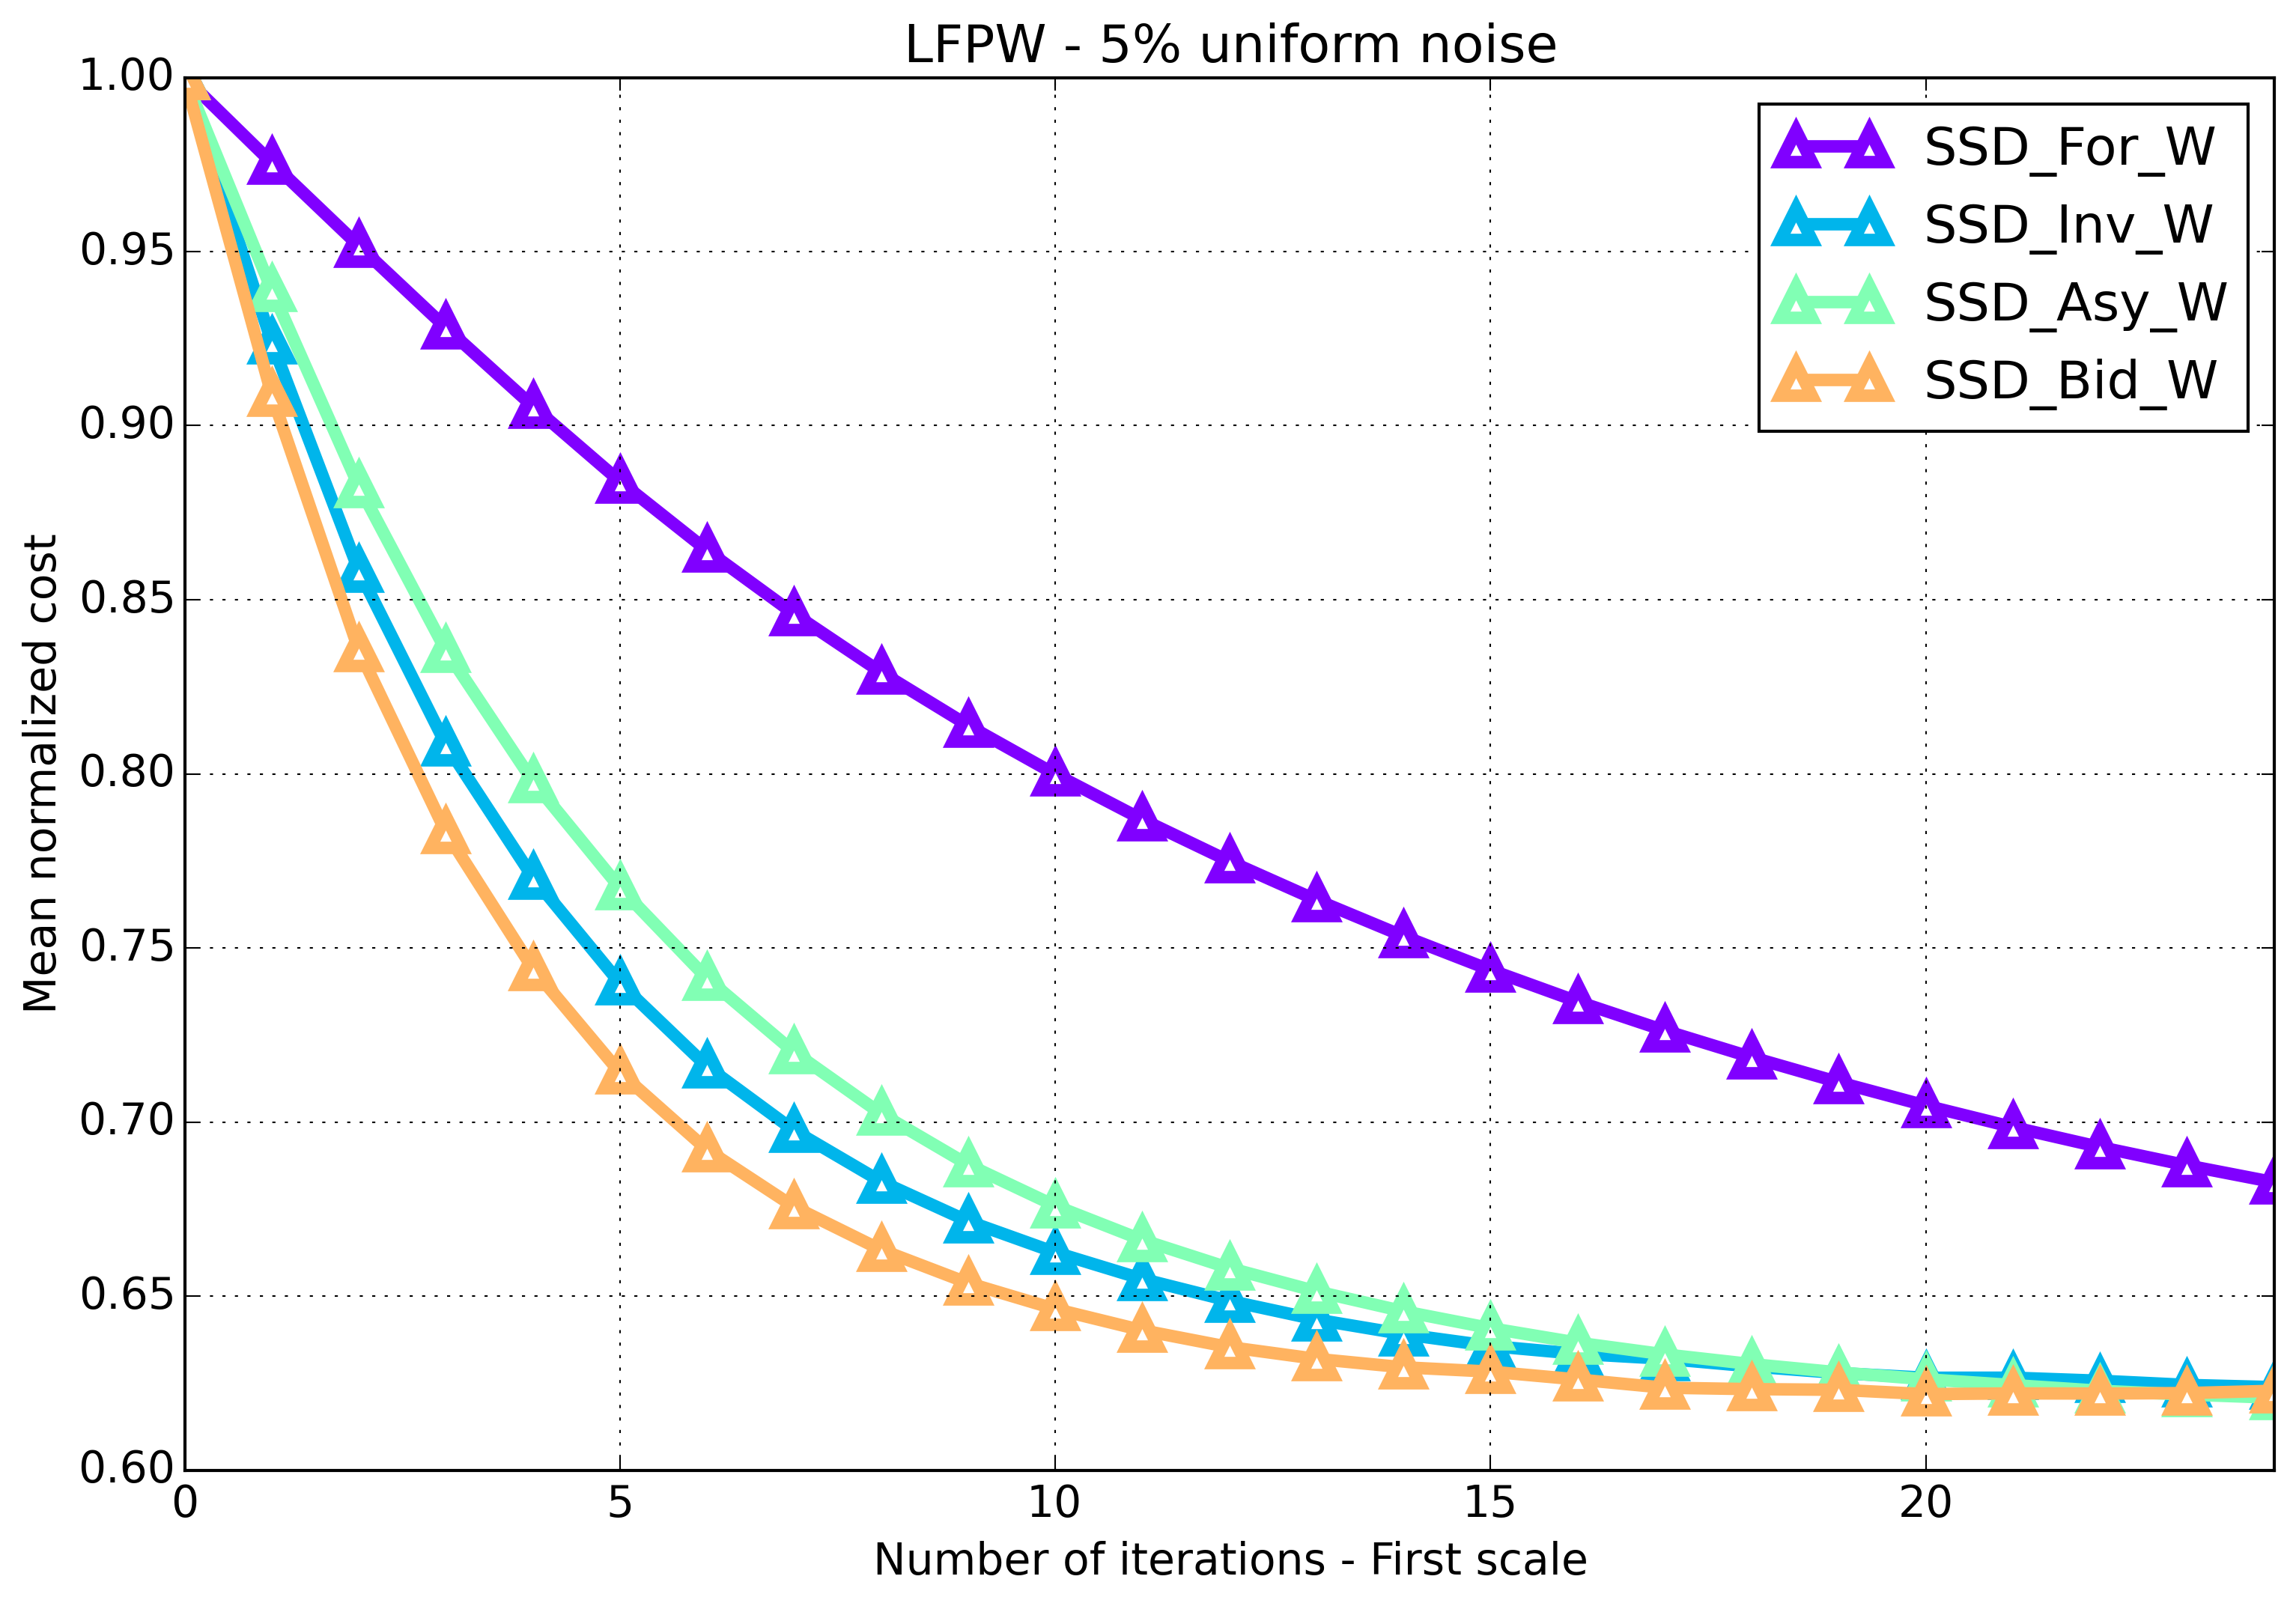
\includegraphics[width=\textwidth]{experiments/algorithms/ssd_w/mean_cost_vs_iters1_ssd_w_5.png}
	    \caption{Mean normalized cost vs number of first scale iterations graph on the LFPW test dataset for all SSD Wiberg algorithms initialized with $5\%$ uniform noise.}
	    \label{fig:mean_cost_vs_iters1_ssd_w_5}
	\end{subfigure}
	\hfill
	\begin{subfigure}{0.48\textwidth}
	    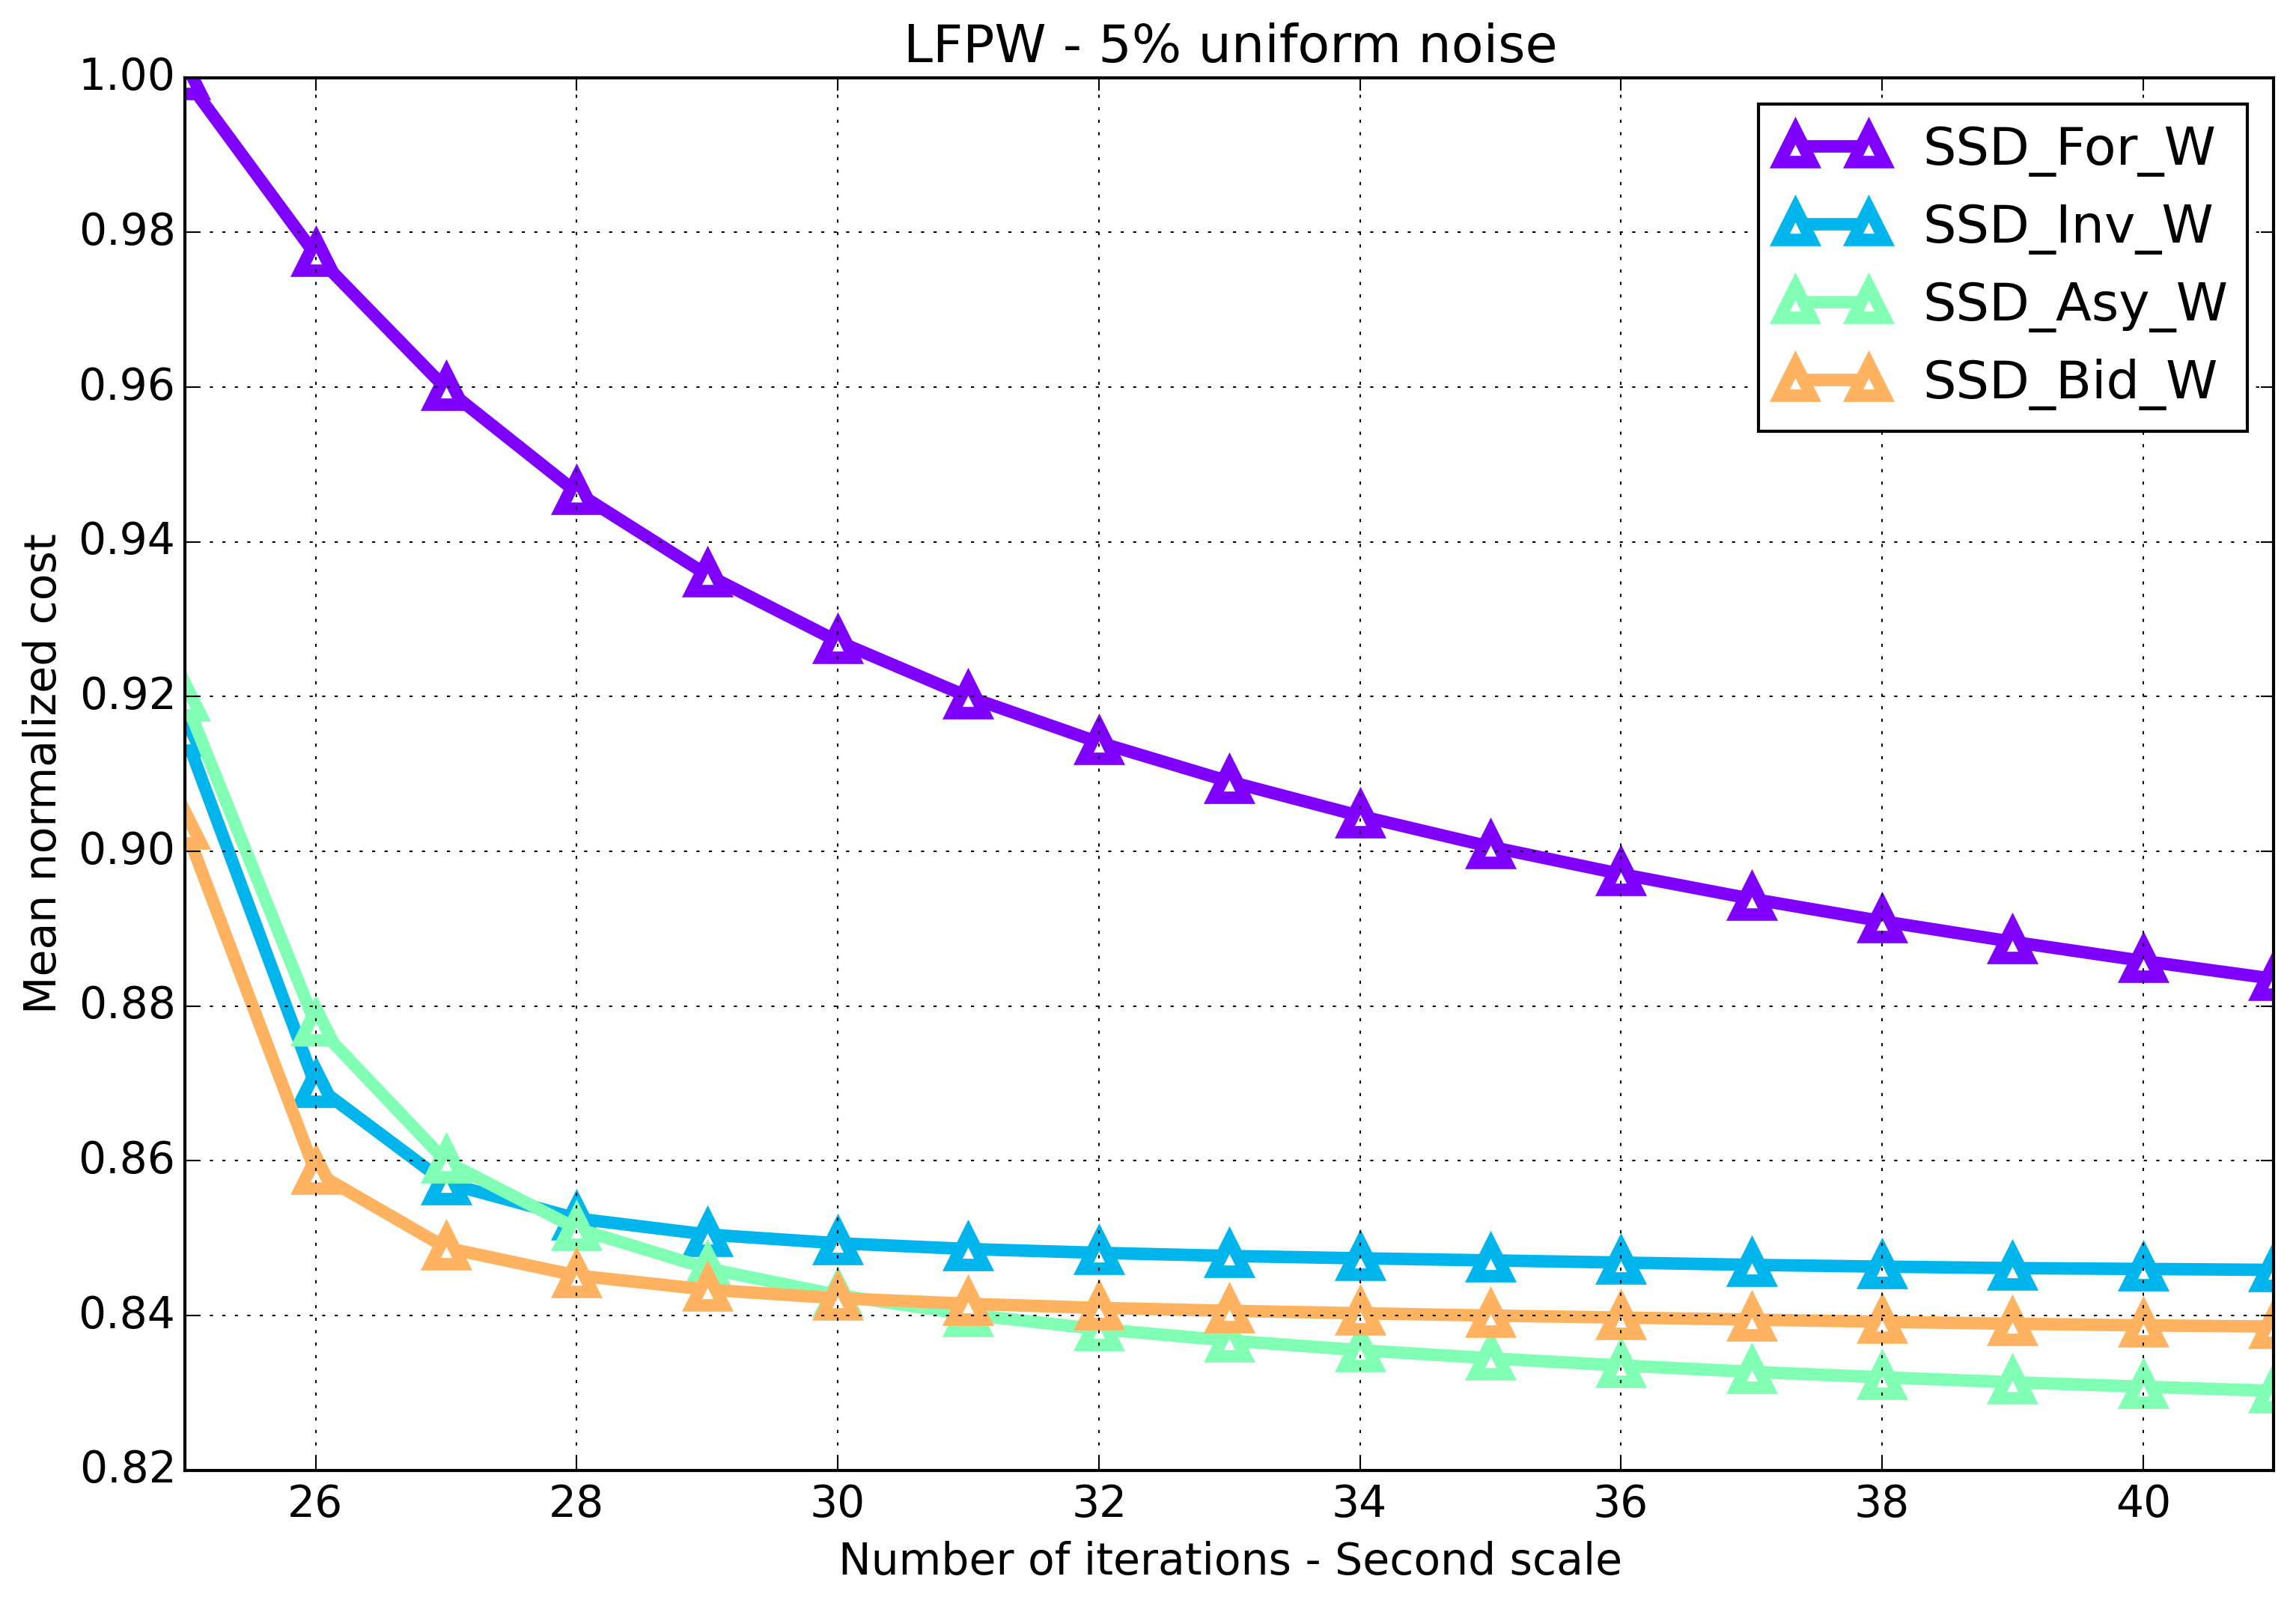
\includegraphics[width=\textwidth]{experiments/algorithms/ssd_w/mean_cost_vs_iters2_ssd_w_5.png}
	    \caption{Mean normalized cost vs number of second scale iterations graph on the LFPW test dataset for all SSD Wiberg algorithms initialized with $5\%$ uniform noise.}
	    \label{fig:mean_cost_vs_iters2_ssd_w_5}
	\end{subfigure}
	\label{fig:ssd_w_5}
	\caption{}
\end{figure*}


\subsubsection{Project-Out algorithms}


\subsubsection*{Gauss-Newton}

\begin{figure*}[h!]
	\centering
	\begin{subfigure}{0.48\textwidth}
	    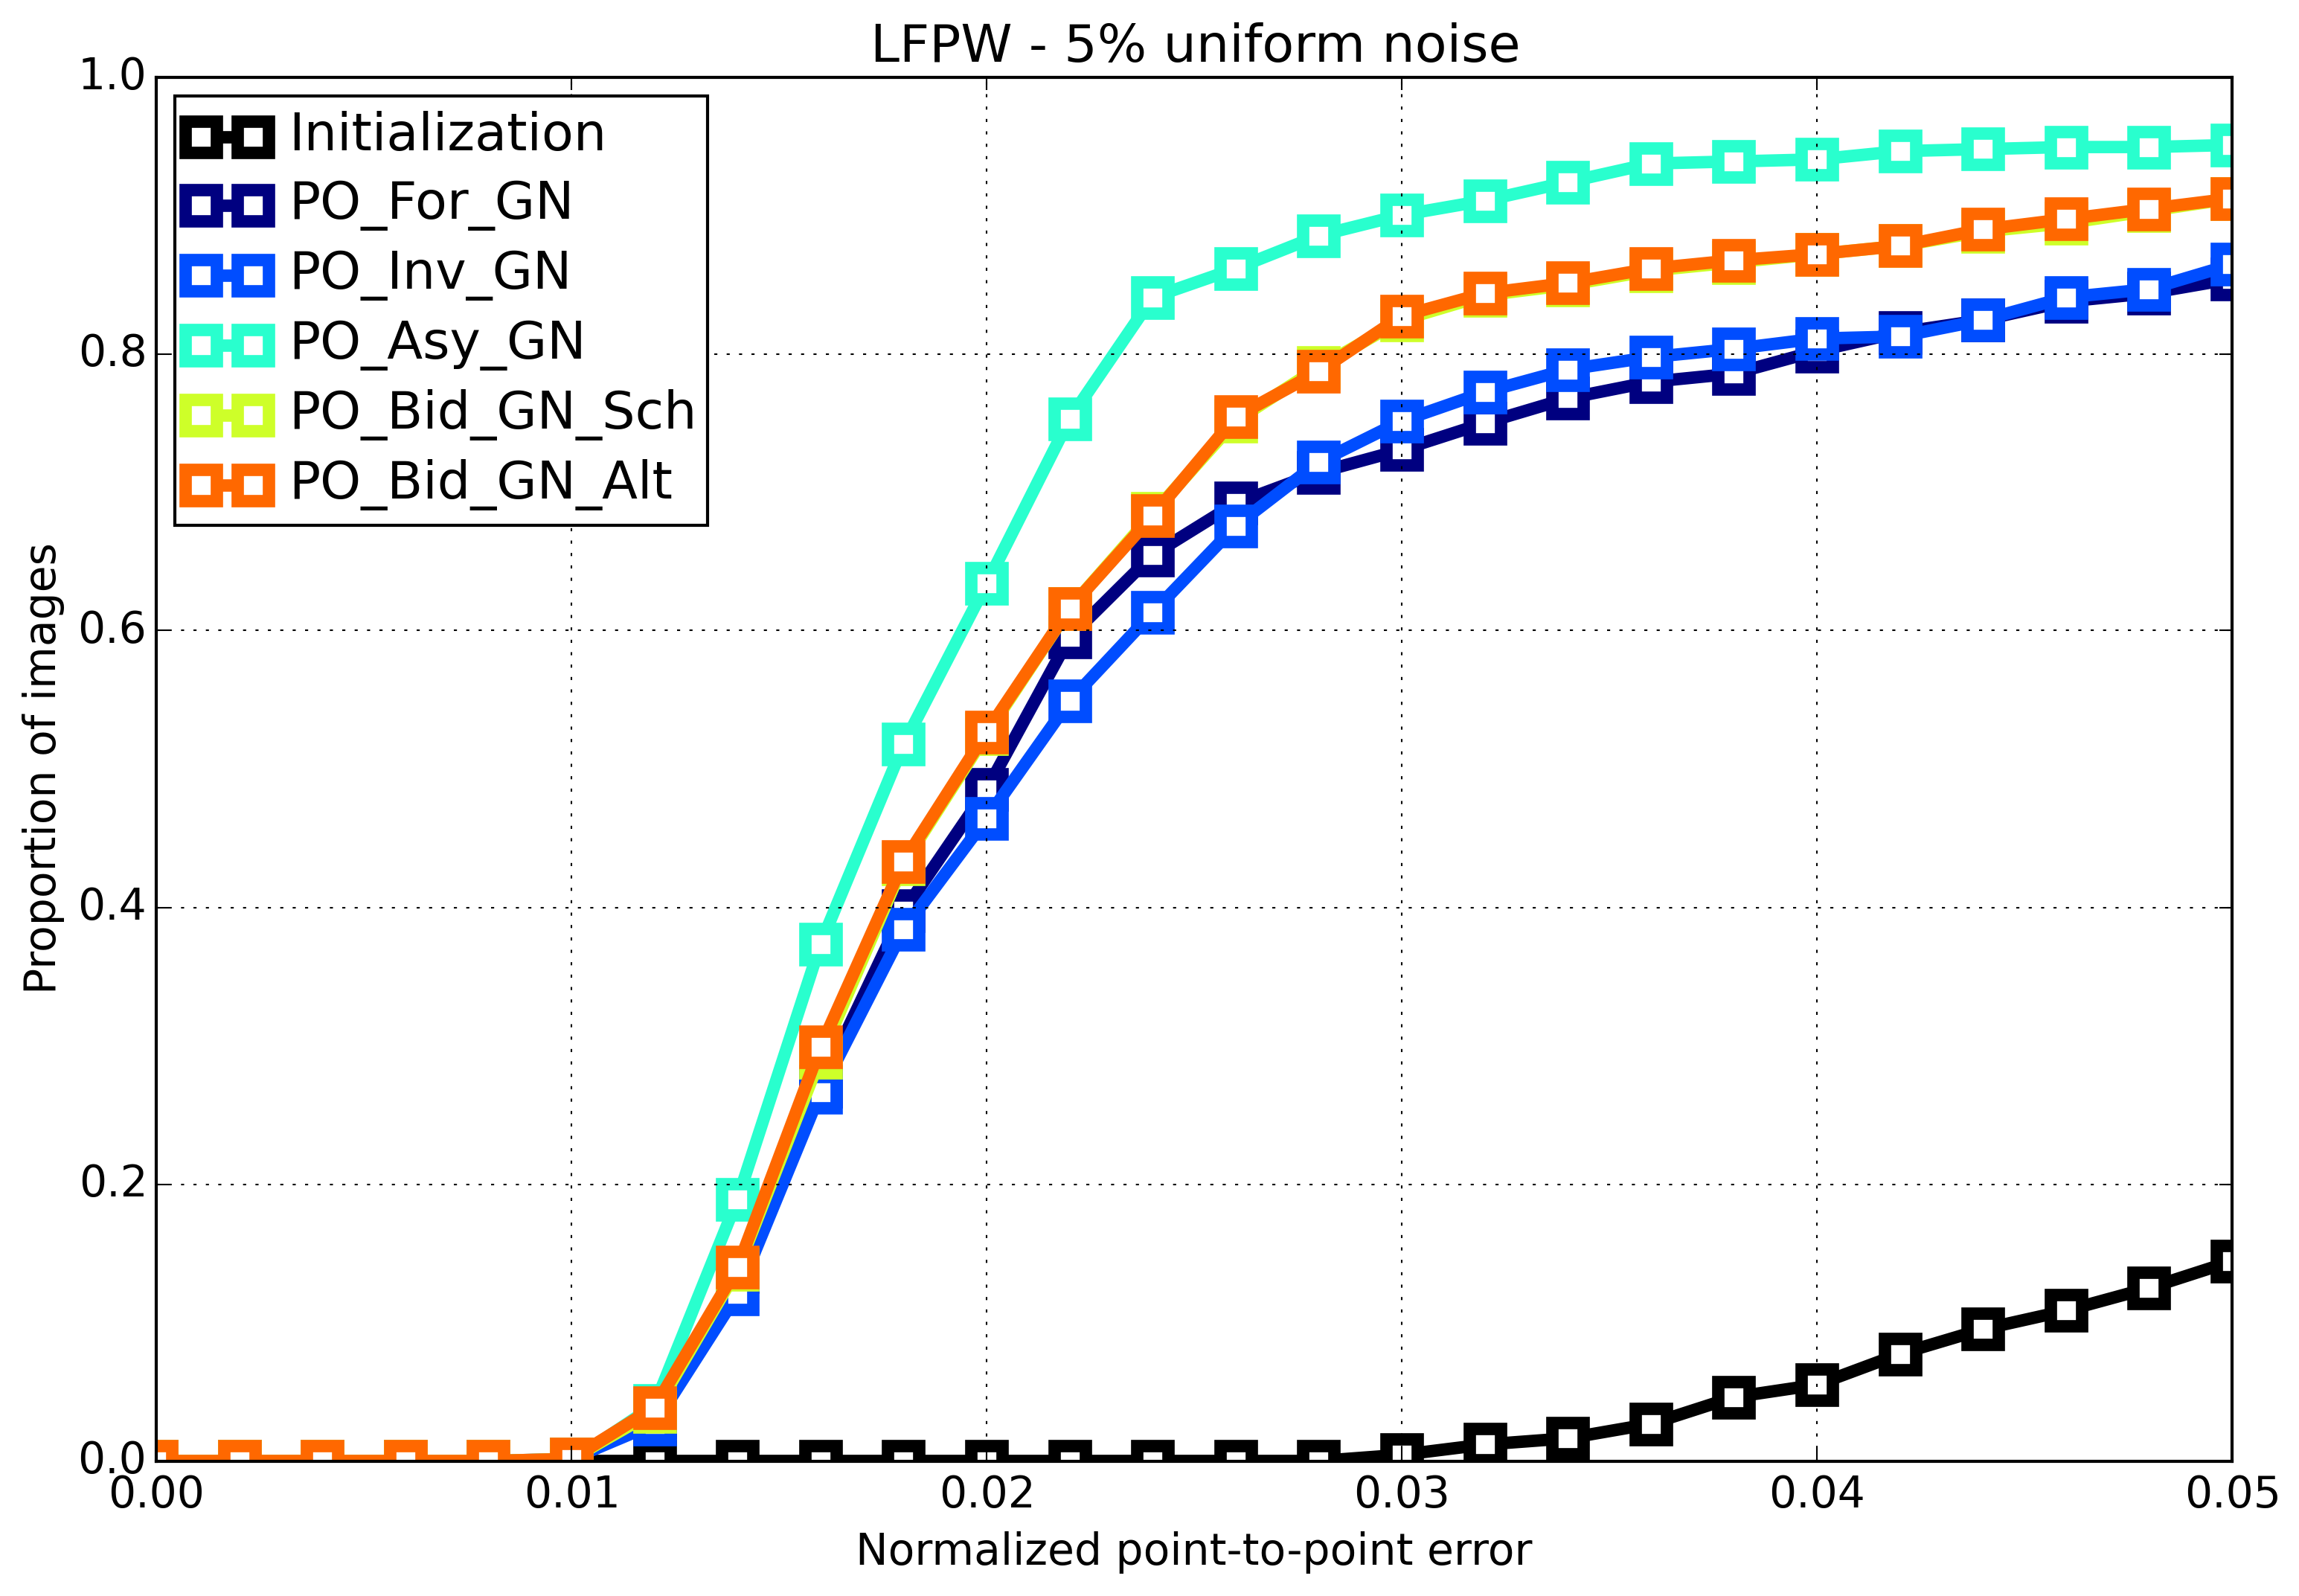
\includegraphics[width=\textwidth]{experiments/algorithms/po_gn/ced_po_gn_5.png}
	    \caption{Cumulative Error Distribution graph on the LFPW test dataset for all Project-Out Gauss-Newton algorithms initialized with $5\%$ uniform noise.}
	    \label{fig:ced_po_gn_5}
	\end{subfigure}
	\hfill
	\begin{subfigure}{0.48\textwidth}
	    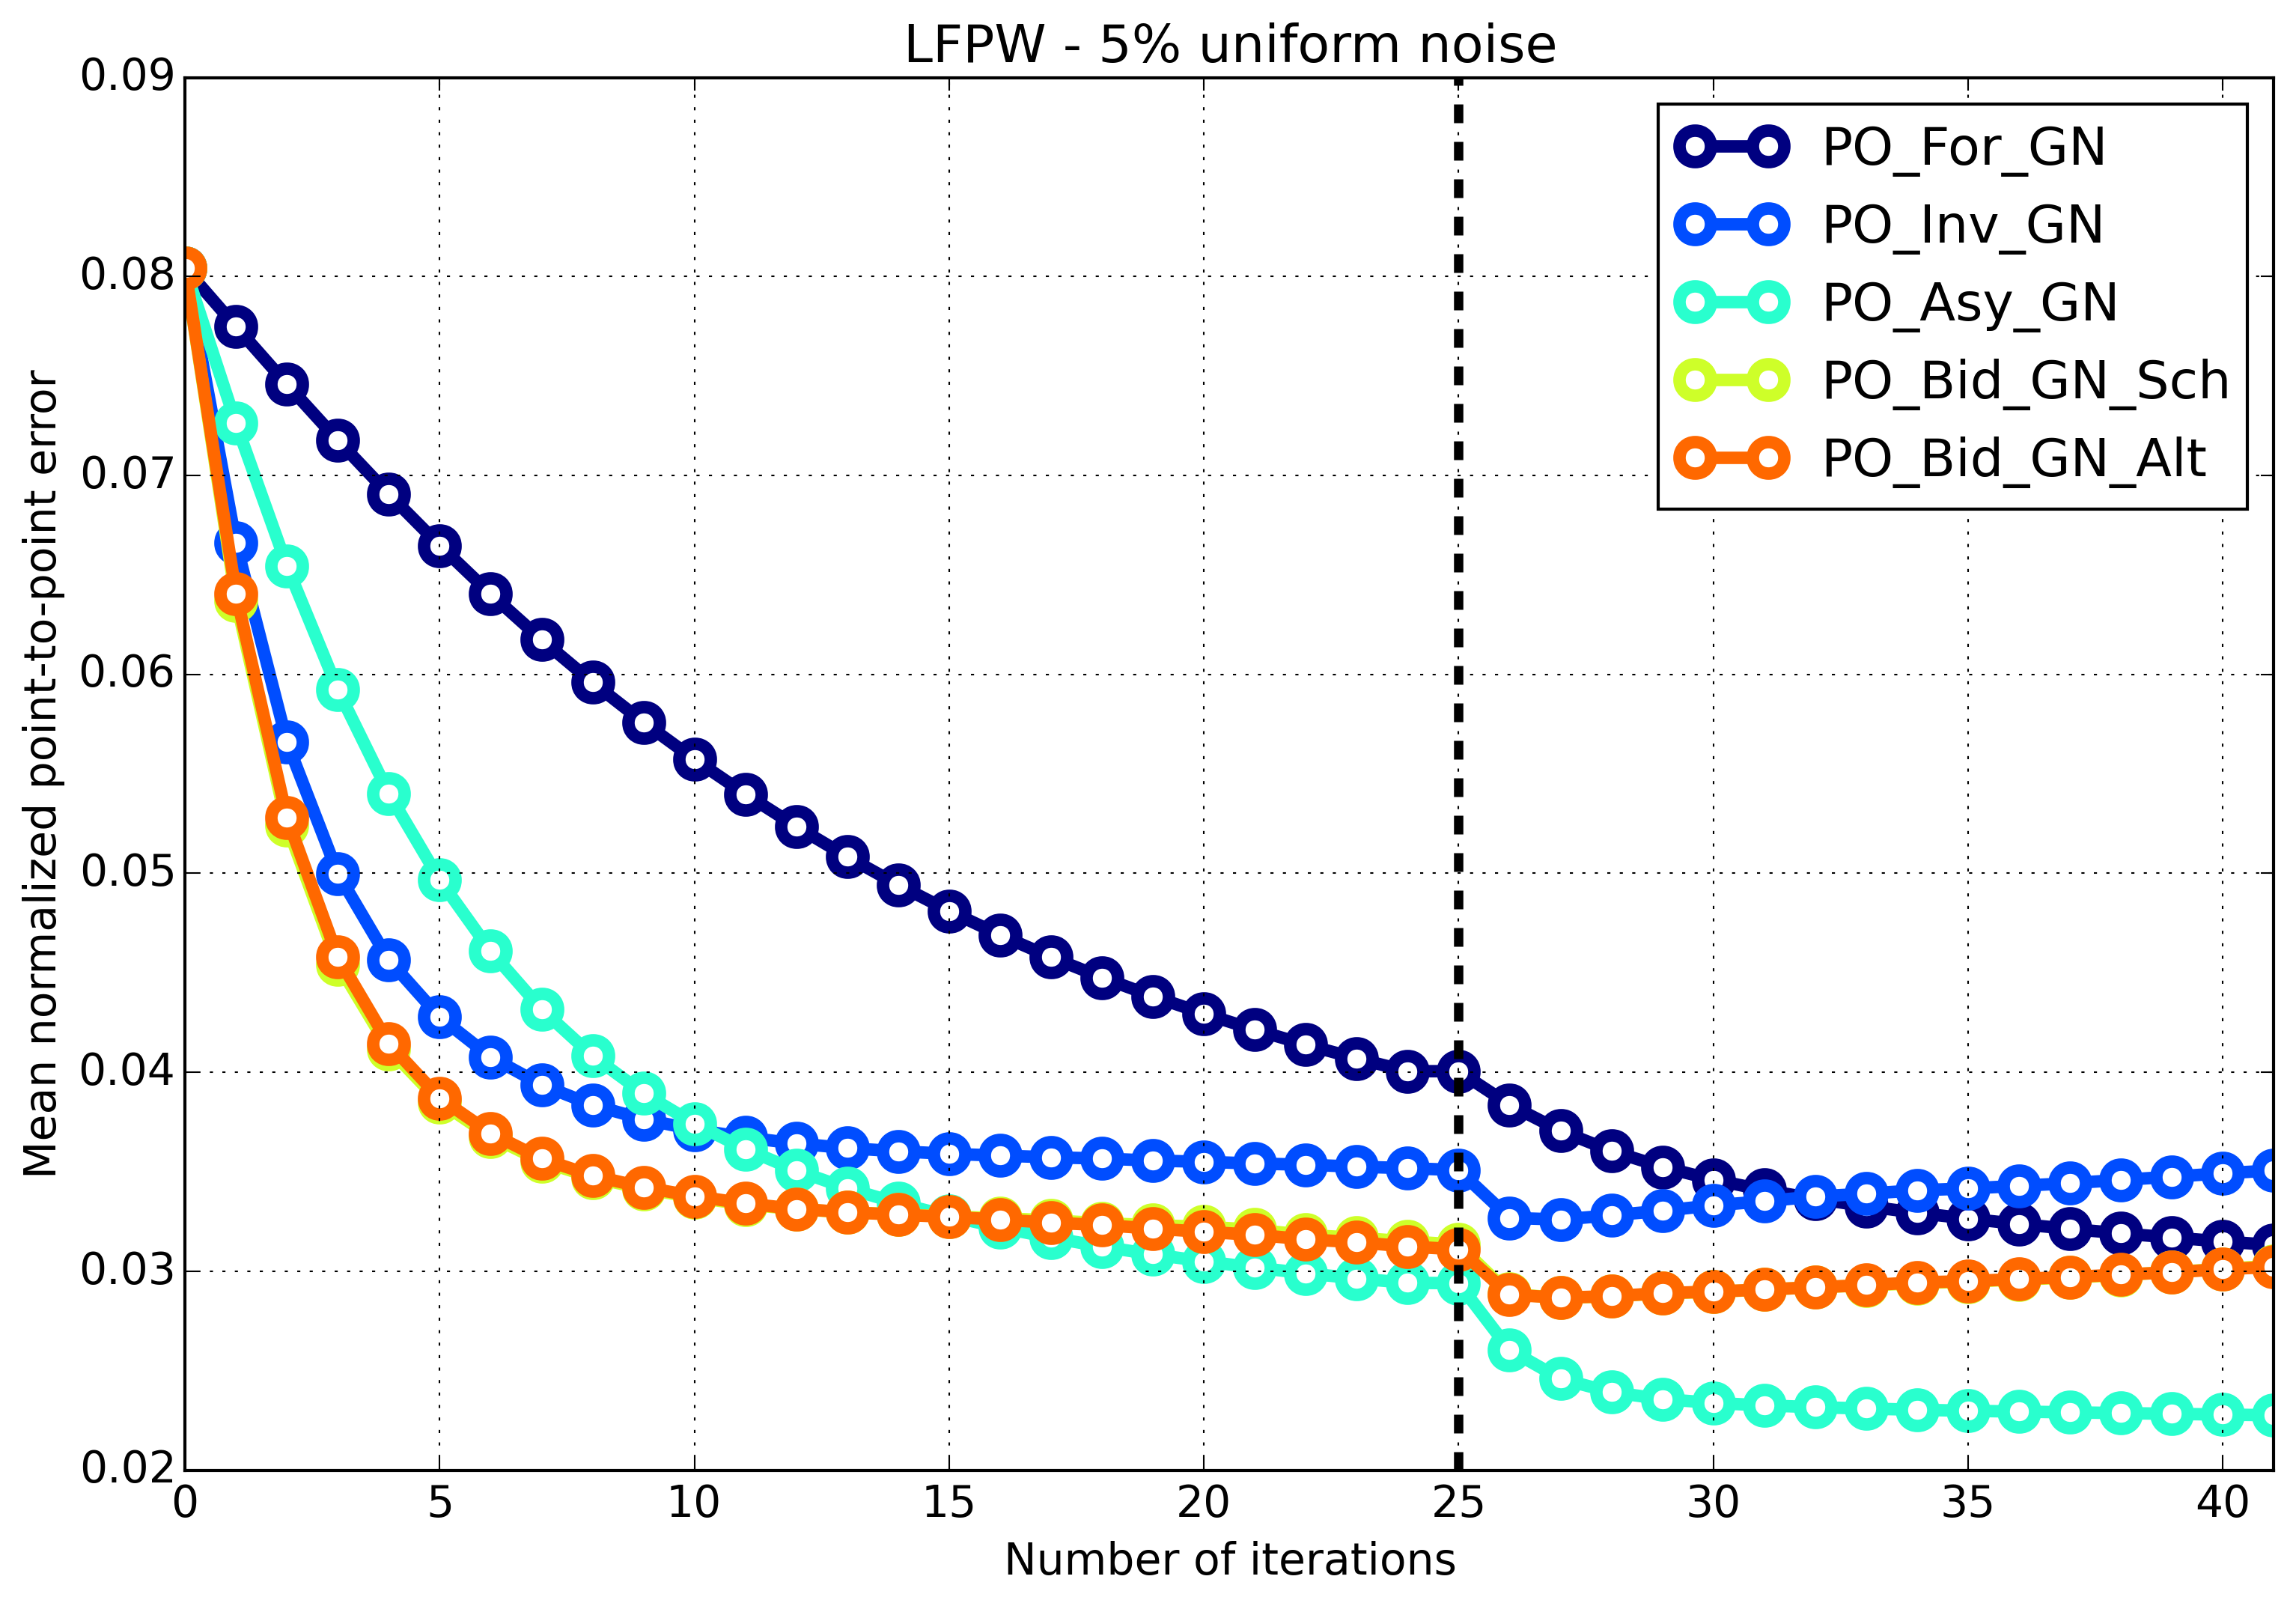
\includegraphics[width=\textwidth]{experiments/algorithms/po_gn/mean_error_vs_iters_po_gn_5.png}
	    \caption{Mean normalized point-to-point error vs number of iterations graph on the LFPW test dataset for all Project-Out Gauss-Newton algorithms initialized with $5\%$ uniform noise.}
	    \label{fig:mean_error_vs_iters_po_gn_5}
	\end{subfigure}
	\par\medskip
	\begin{subfigure}{0.48\textwidth}
	    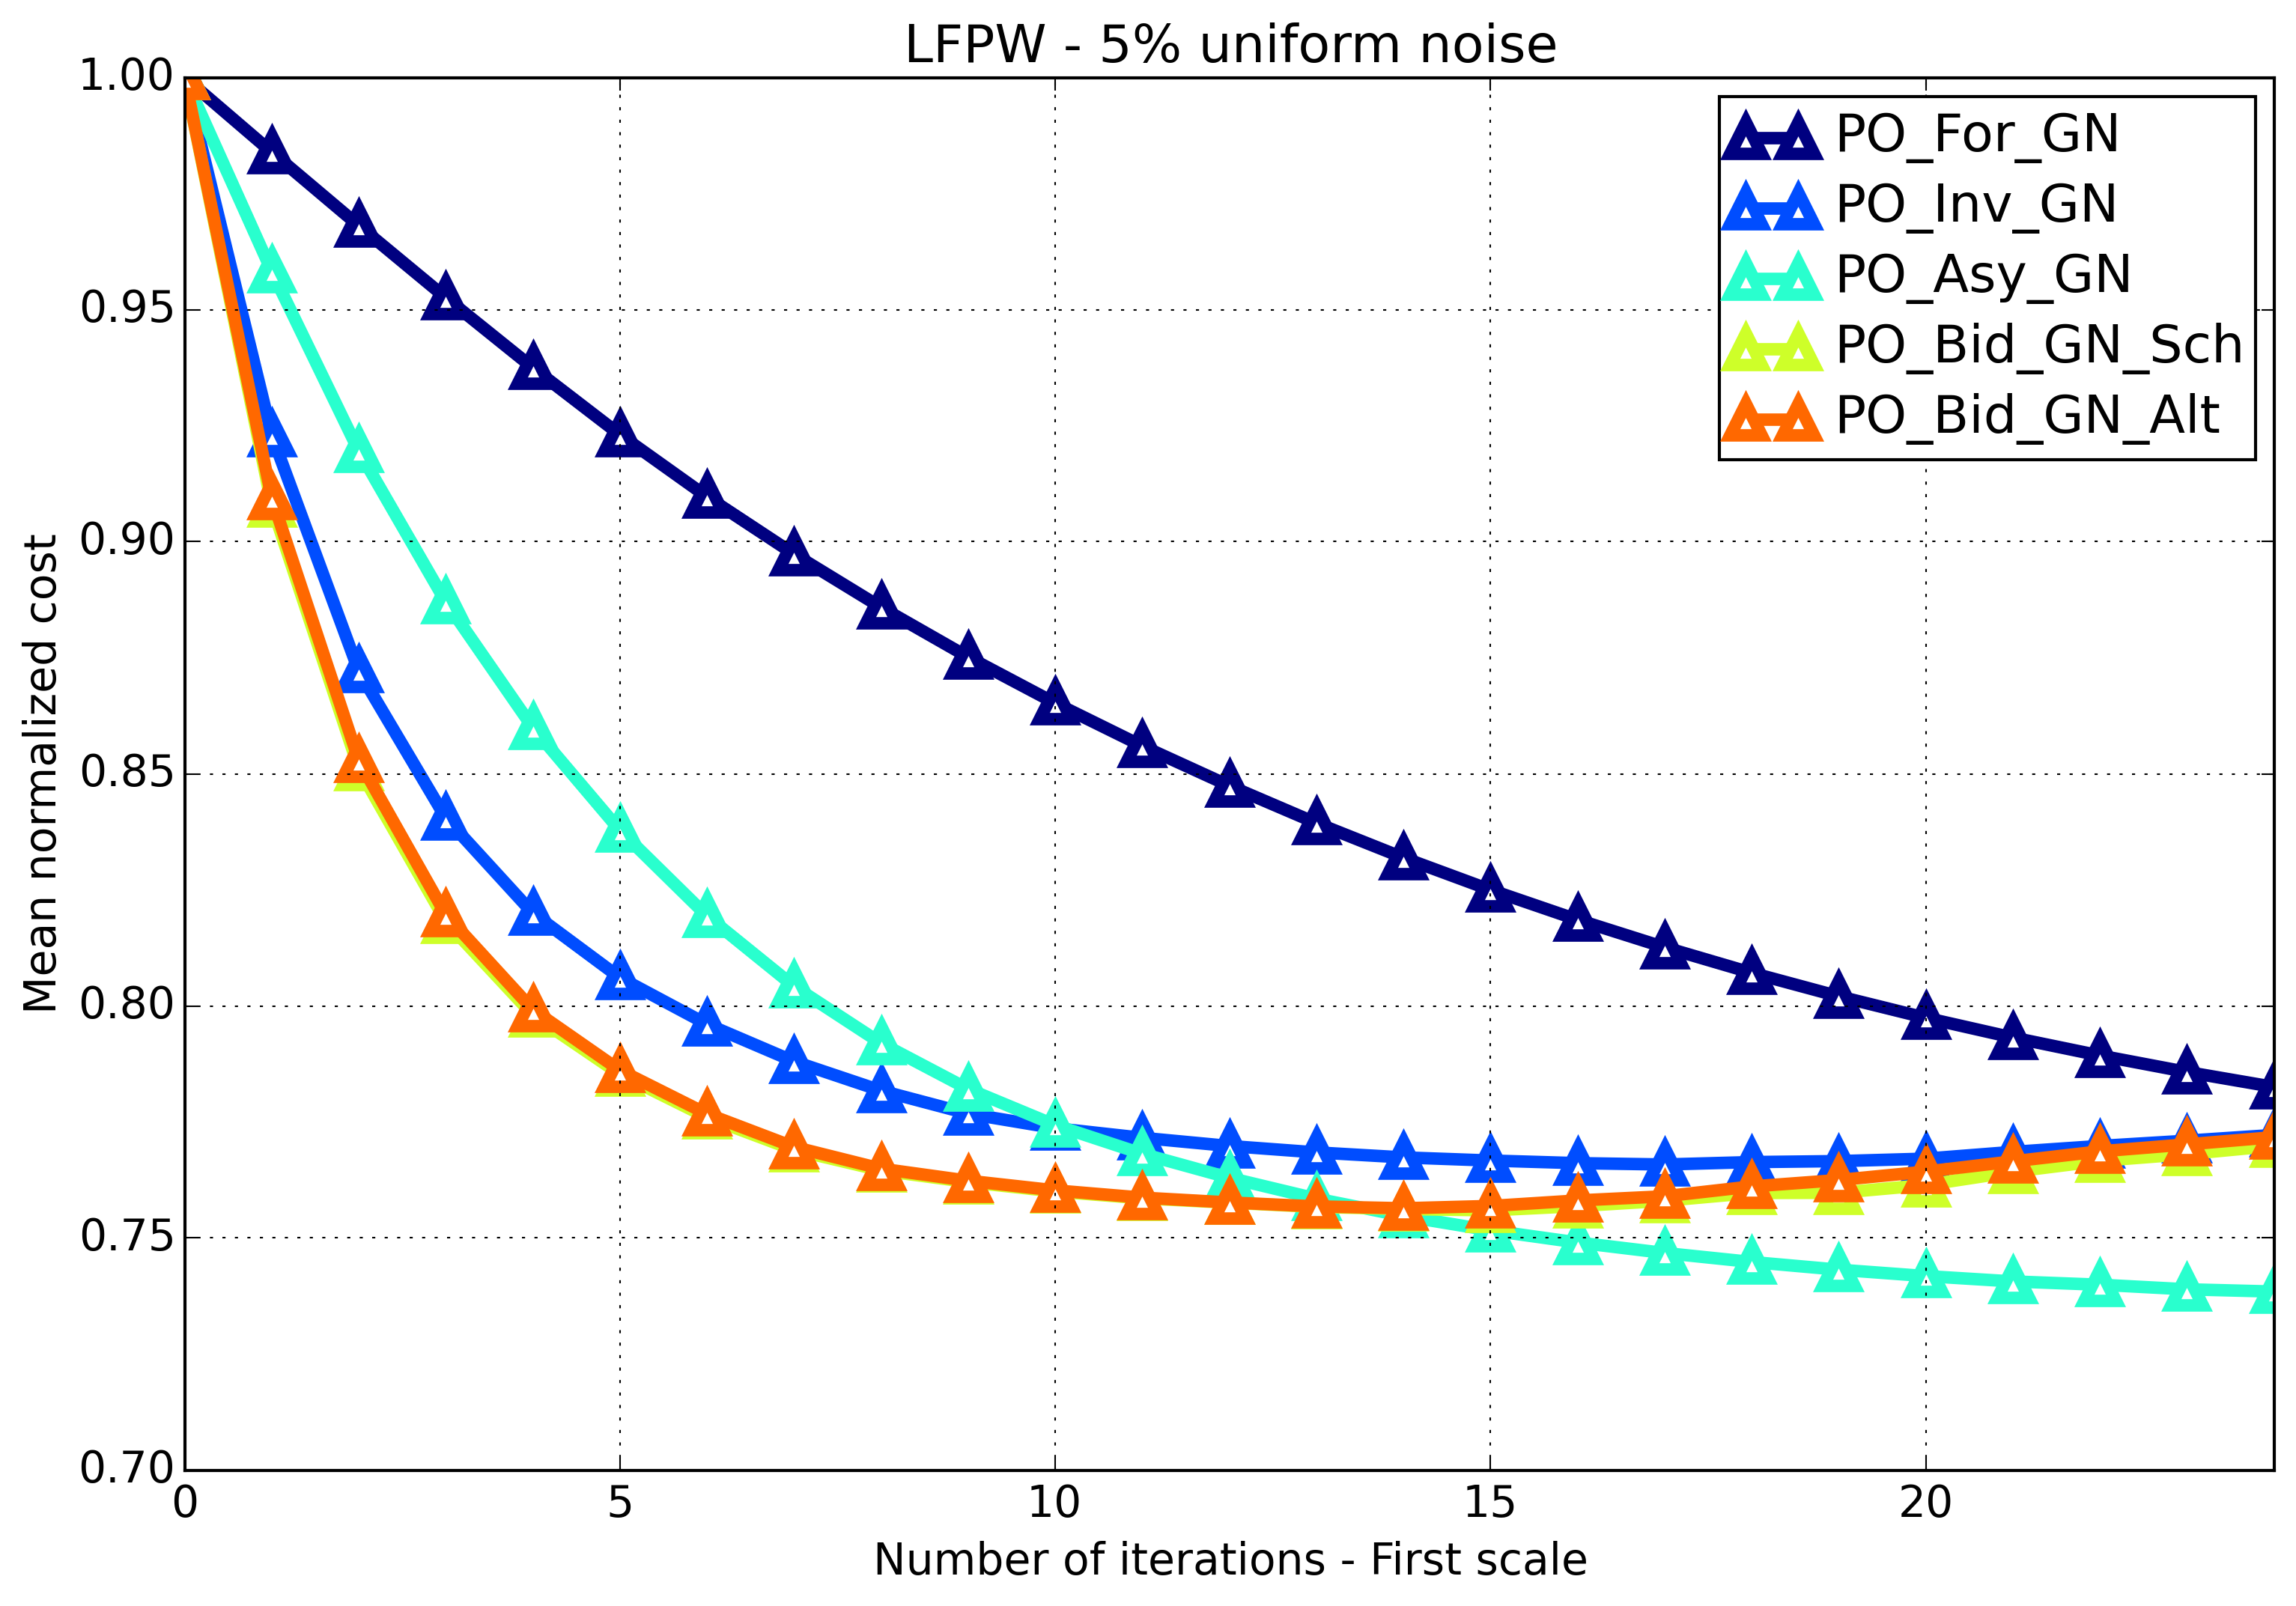
\includegraphics[width=\textwidth]{experiments/algorithms/po_gn/mean_cost_vs_iters1_po_gn_5.png}
	    \caption{Mean normalized cost vs number of first scale iterations graph on the LFPW test dataset for all Project-Out Gauss-Newton algorithms initialized with $5\%$ uniform noise.}
	    \label{fig:mean_cost_vs_iters1_po_gn_5}
	\end{subfigure}
	\hfill
	\begin{subfigure}{0.48\textwidth}
	    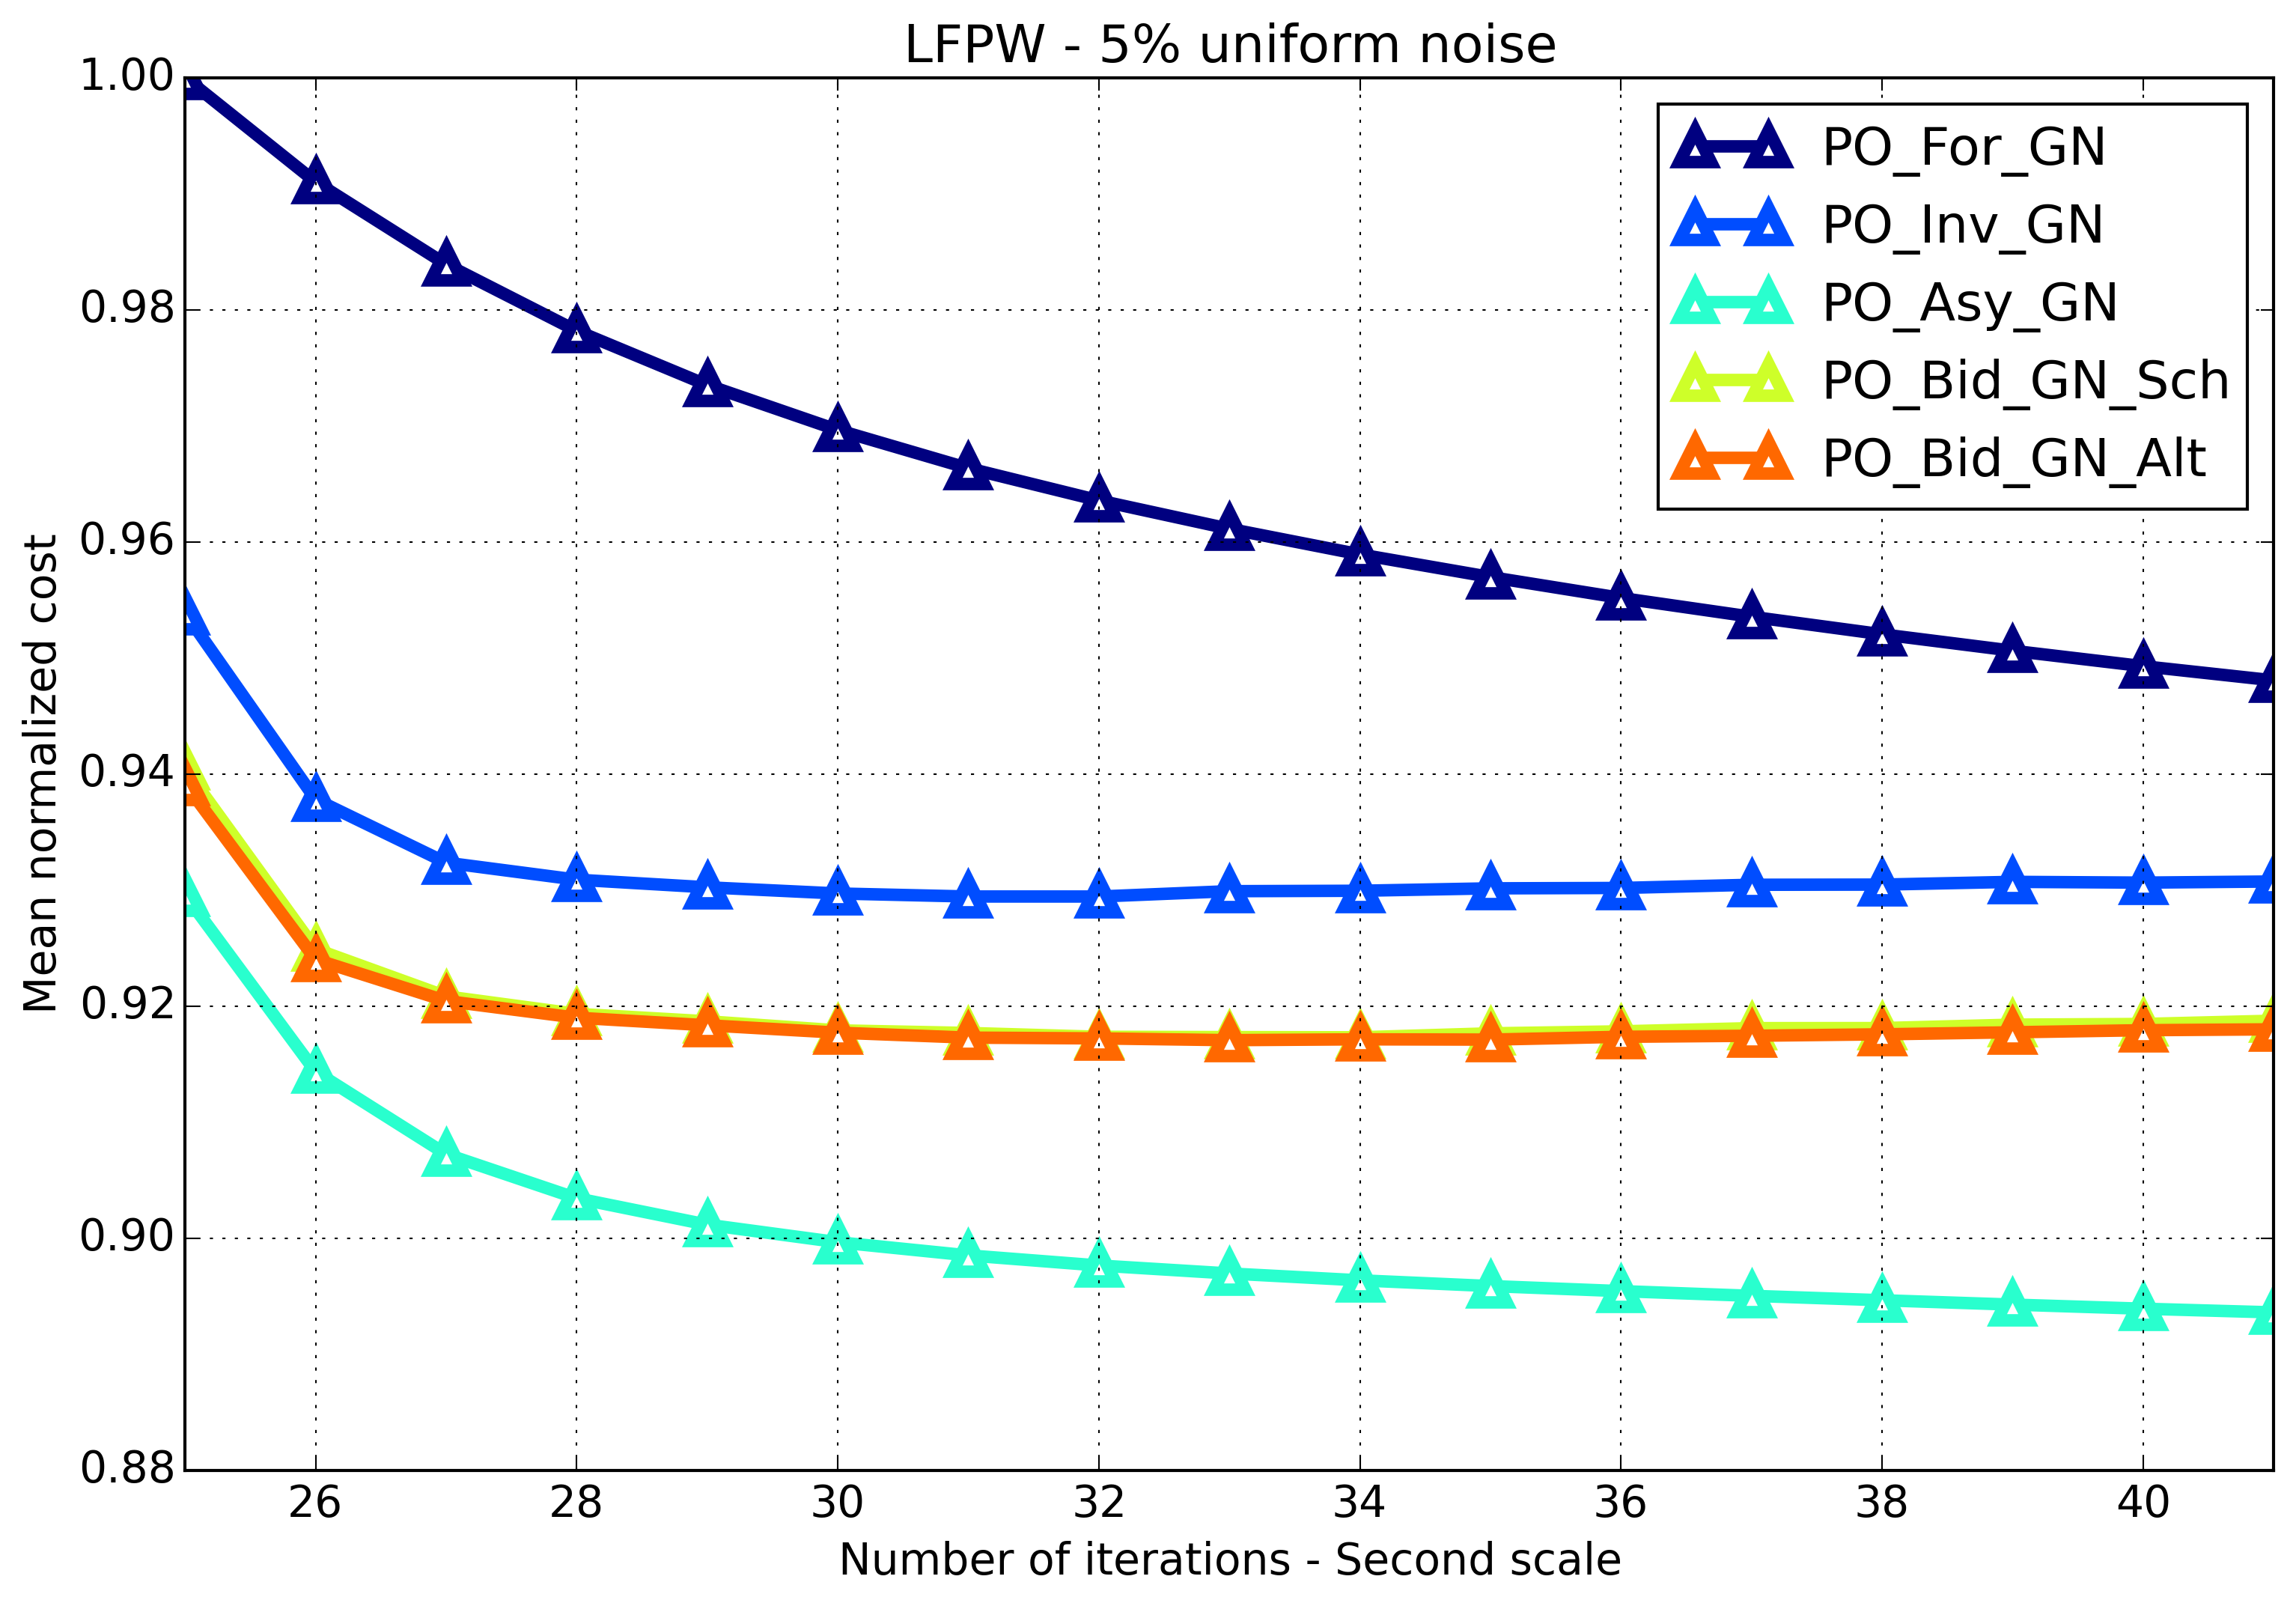
\includegraphics[width=\textwidth]{experiments/algorithms/po_gn/mean_cost_vs_iters2_po_gn_5.png}
	    \caption{Mean normalized cost vs number of second scale iterations graph on the LFPW test dataset for all Project-Out Gauss-Newton algorithms initialized with $5\%$ uniform noise.}
	    \label{fig:mean_cost_vs_iters2_po_gn_5}
	\end{subfigure}
	\label{fig:po_gn_5}
	\caption{}
\end{figure*}


% \subsubsection{Project-Out Newton algorithms}

% \begin{figure}[h!]
%     \centering
%     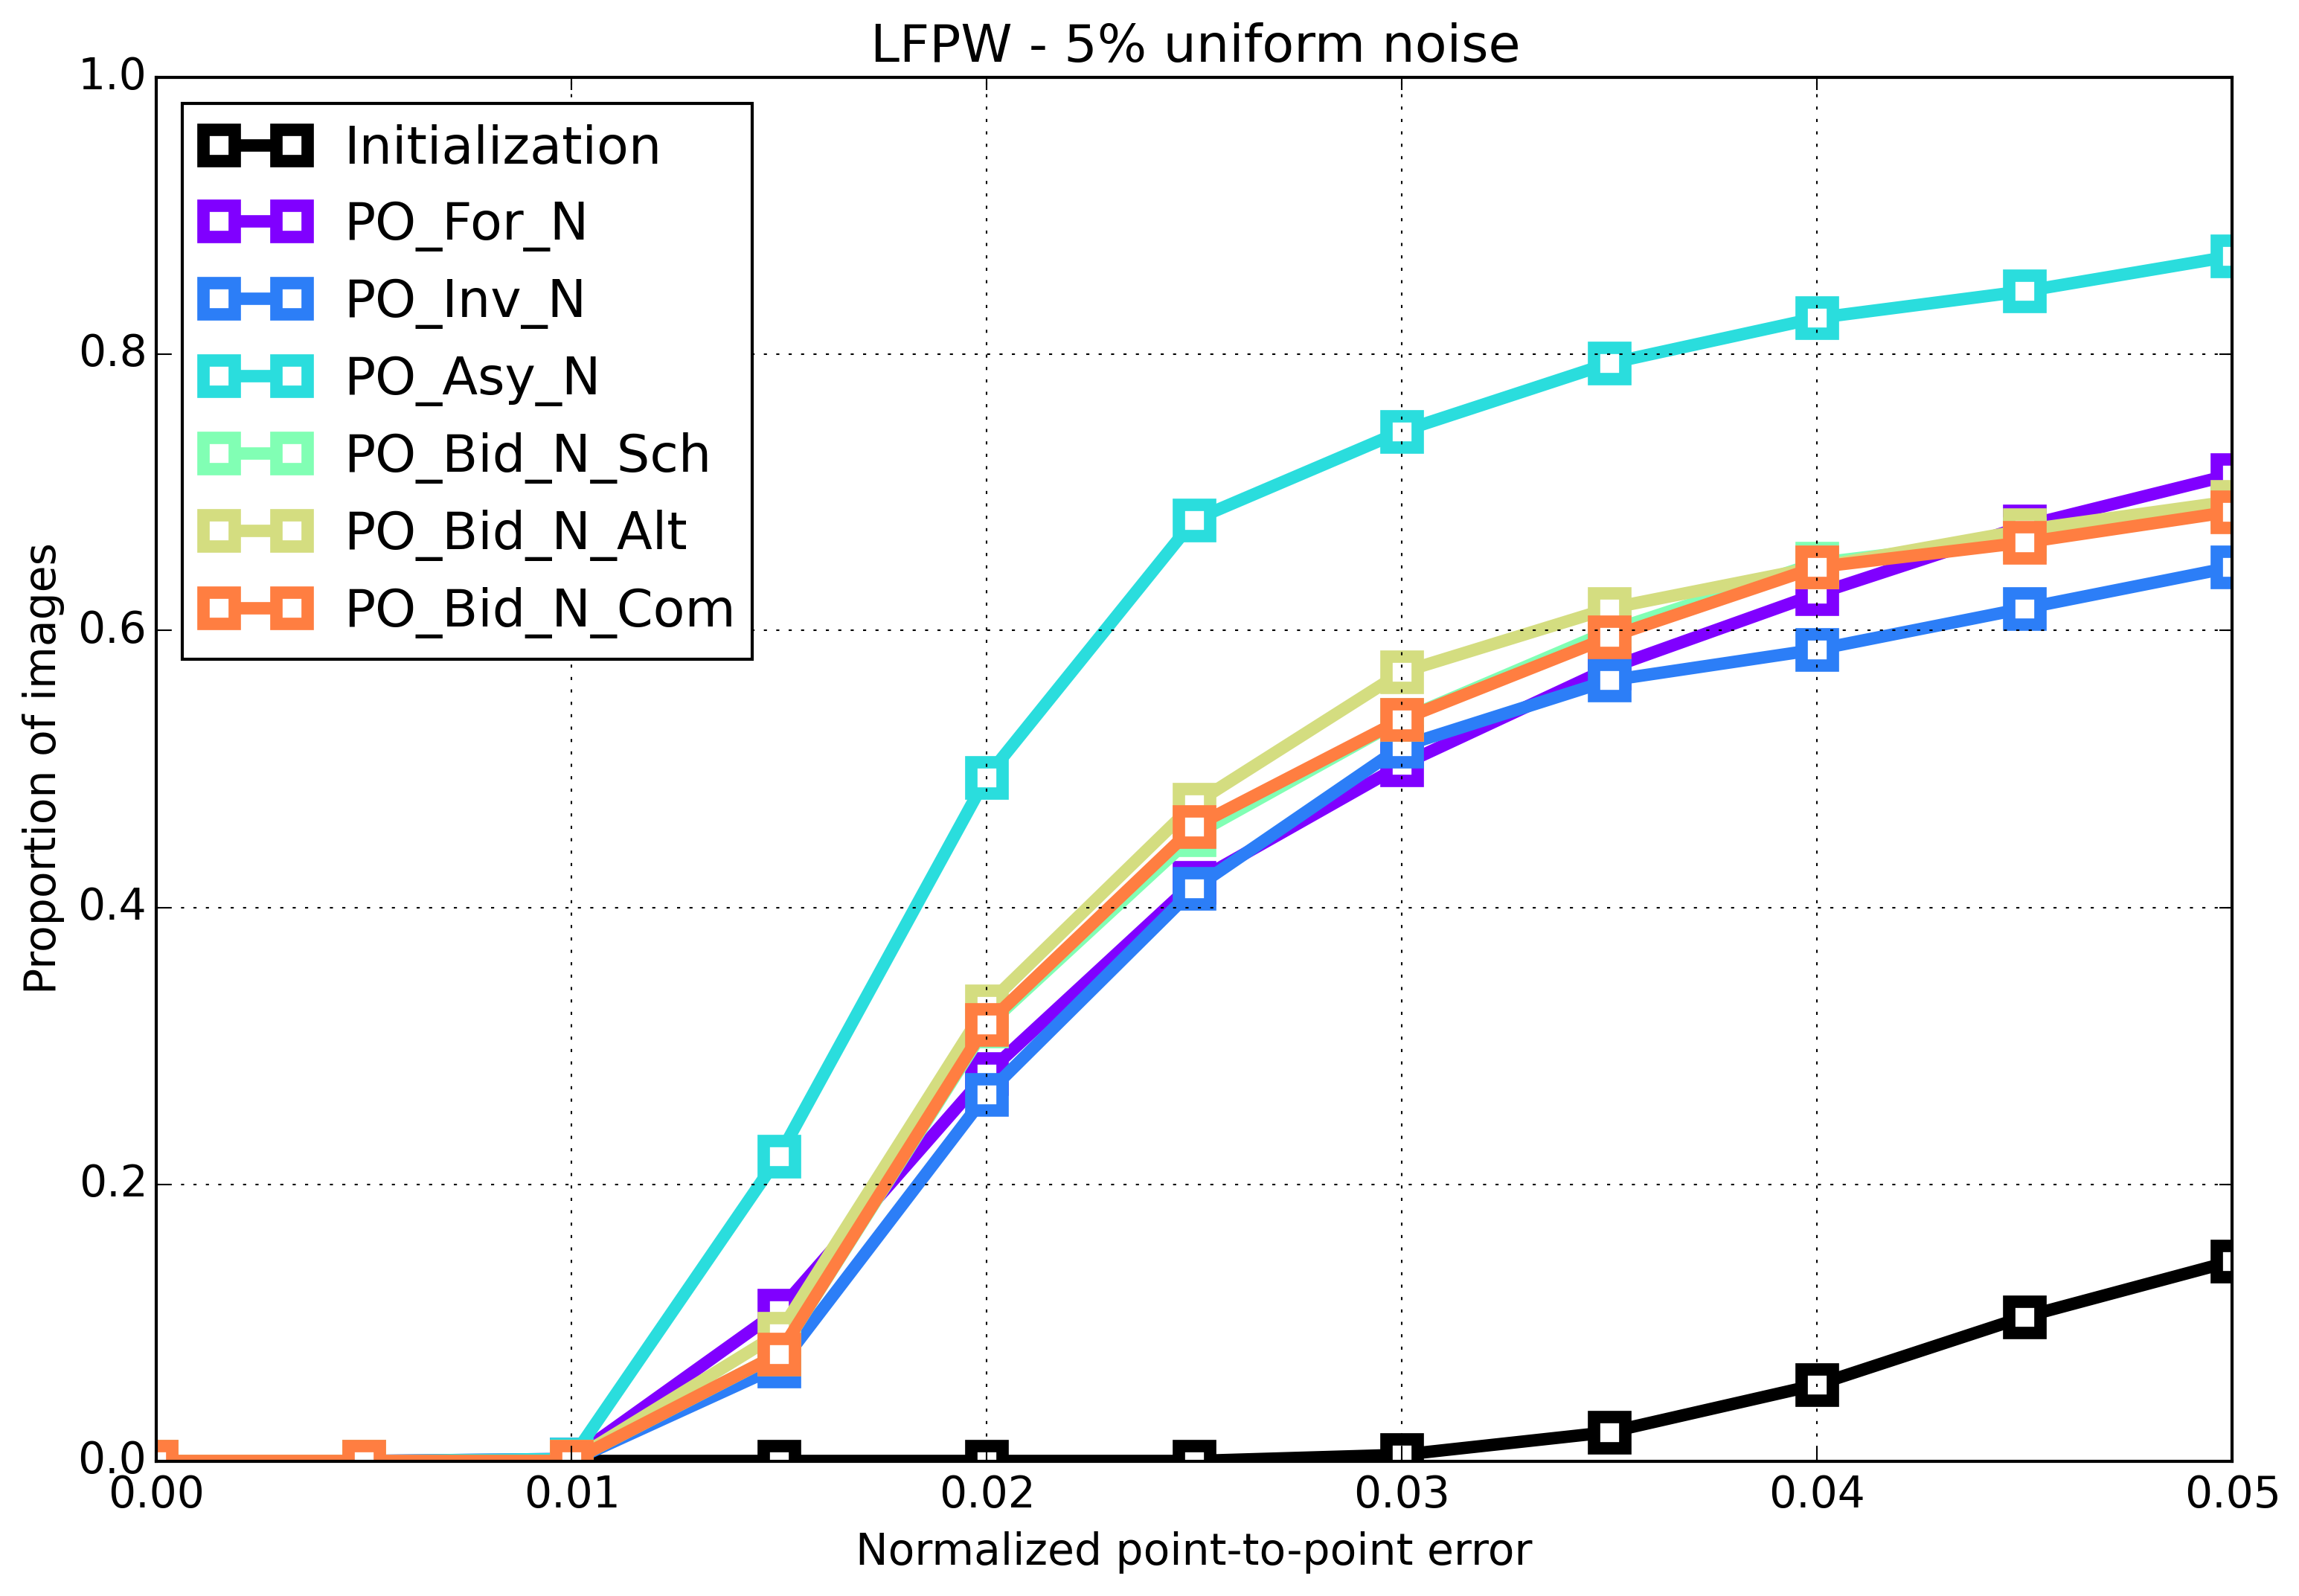
\includegraphics[width=0.50\textwidth]{experiments/algorithms/po_n/ced_po_n_5.png}
%     \caption{CED graph on the LFPW test dataset for all Project-Out Newton algorithms initialized with $4$\% uniform noise.}
%     \label{fig:ced_po_gn_4}
% \end{figure}

% \begin{figure}[h!]
%     \centering
%     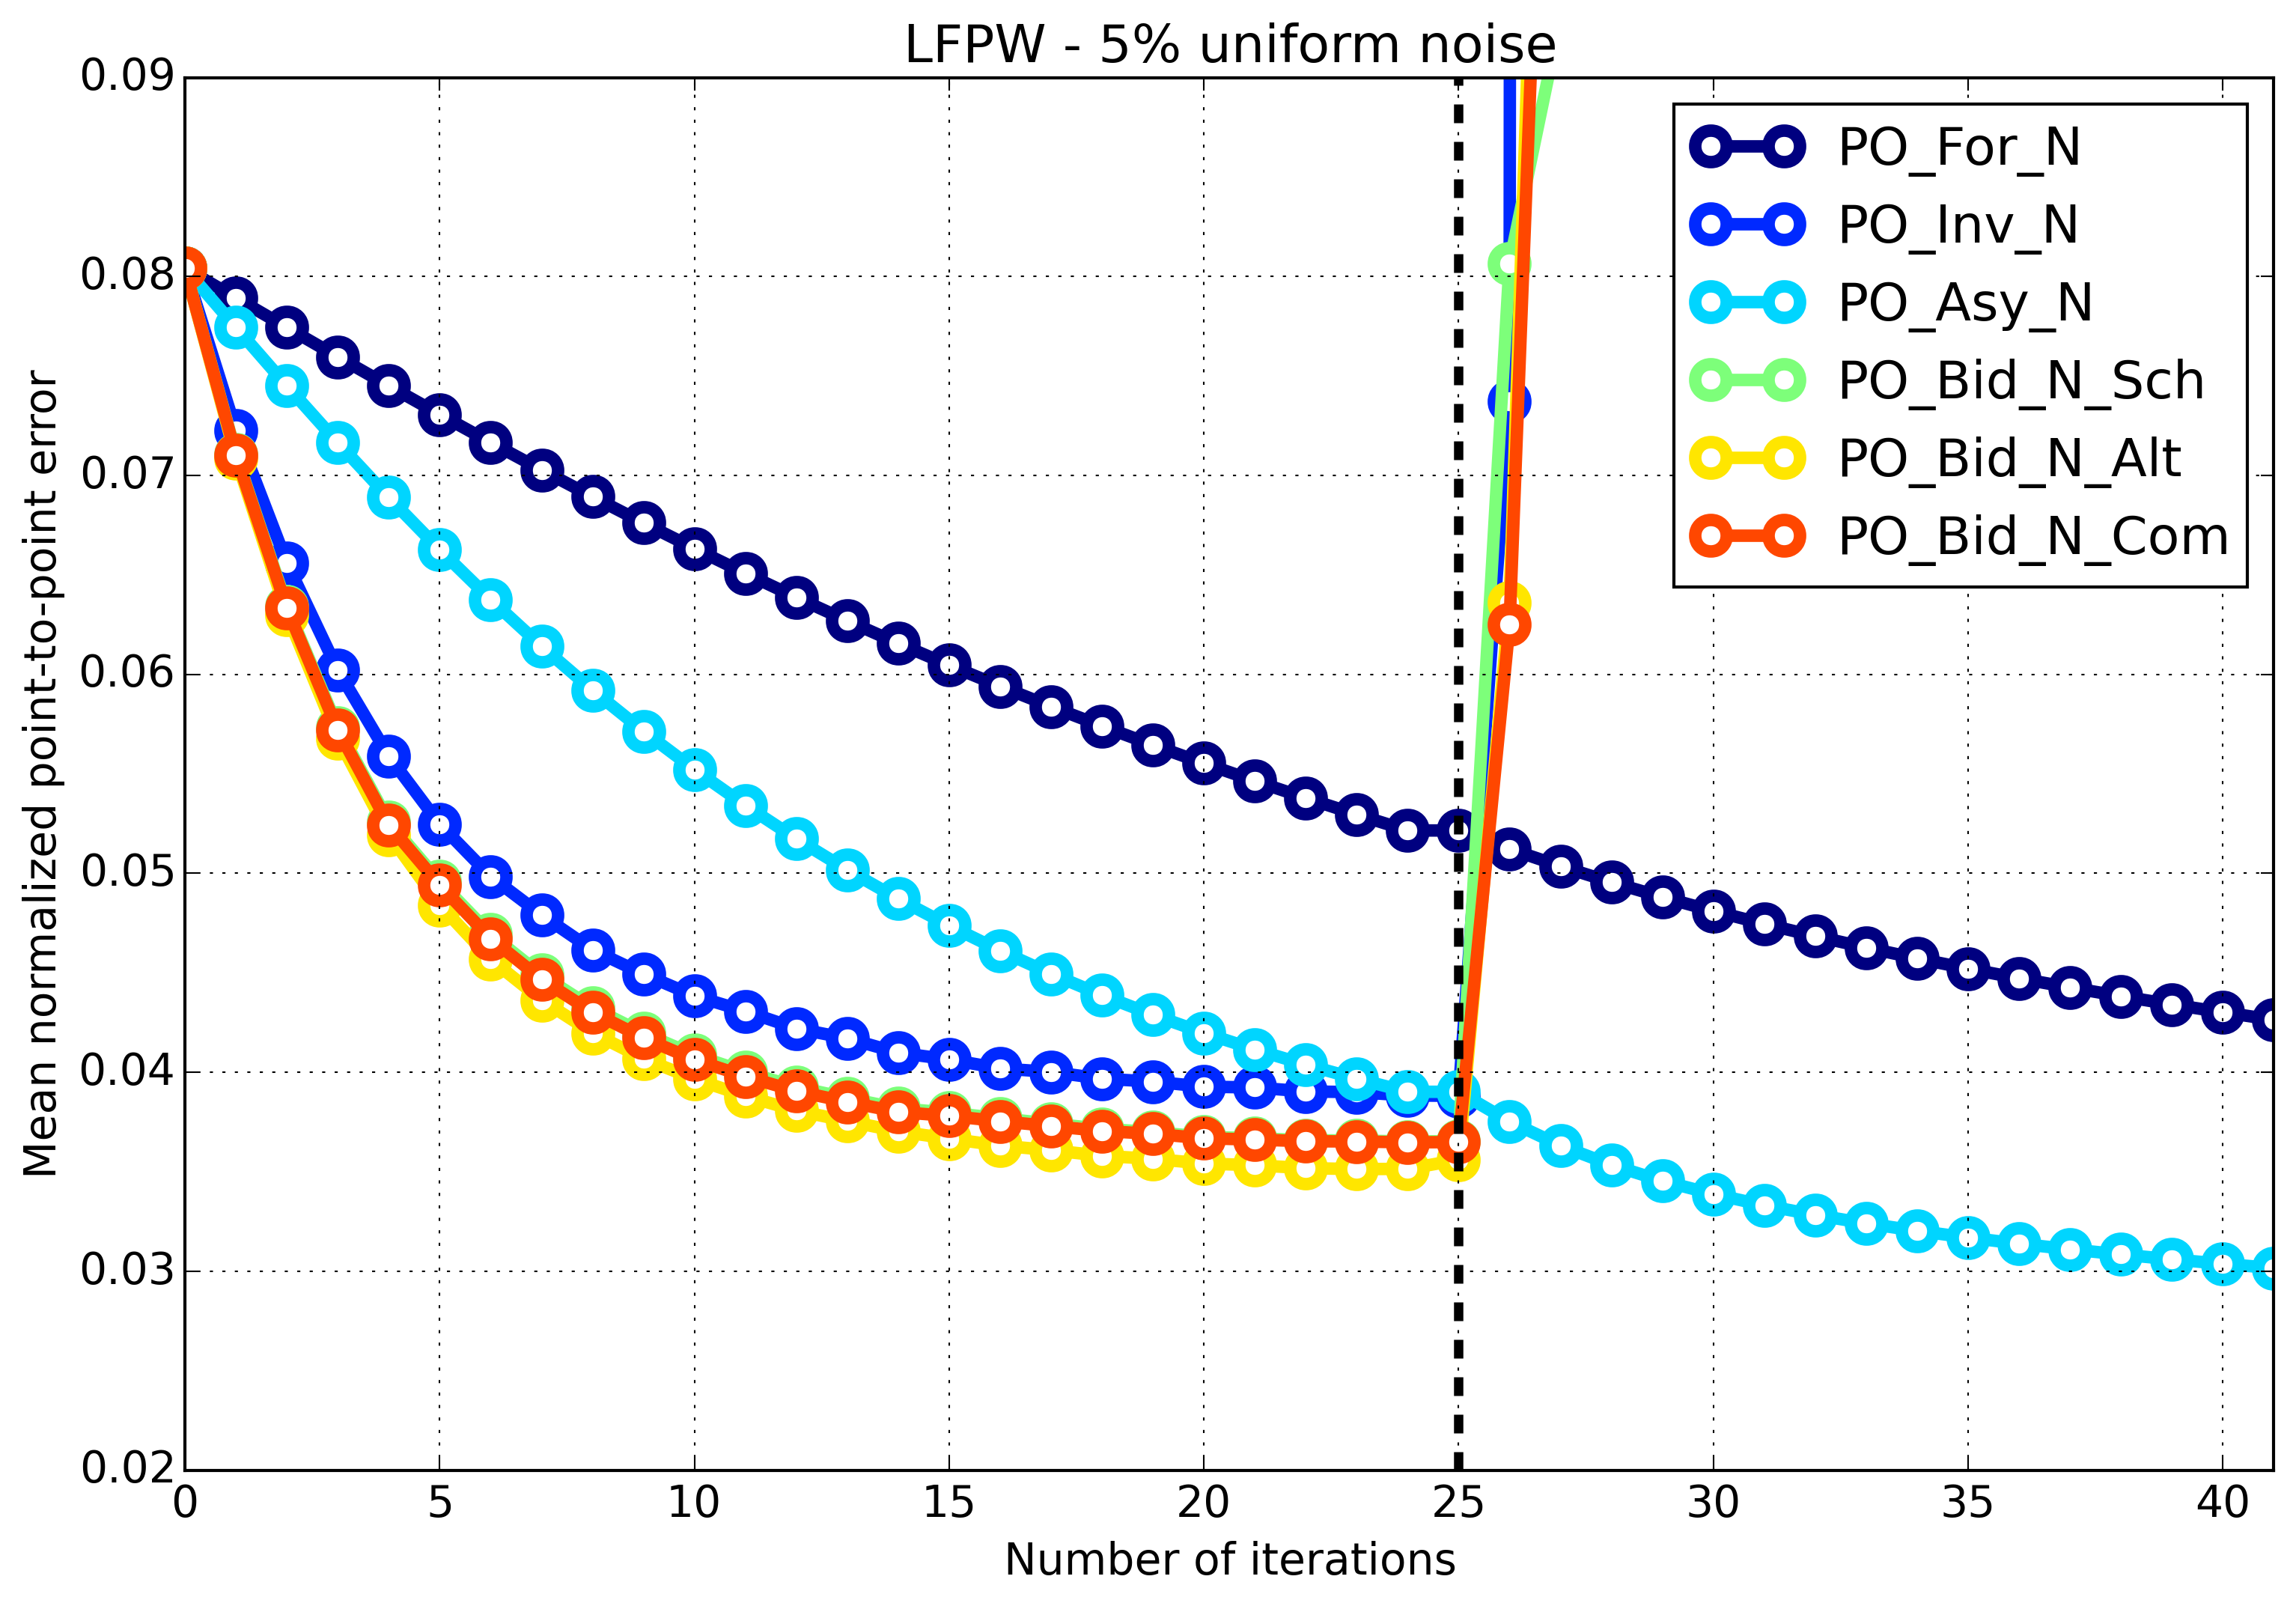
\includegraphics[width=0.50\textwidth]{experiments/algorithms/po_n/mean_error_vs_iters_po_n_5.png}
%     \caption{Mean normalized point-to-point error vs number of iterations graph on the LFPW test dataset for all Project-Out Newton algorithms initialized with $4$\% uniform noise.}
%     \label{fig:mean_error_vs_iters_po_n_4}
% \end{figure}

% \begin{figure}[h!]
%     \centering
%     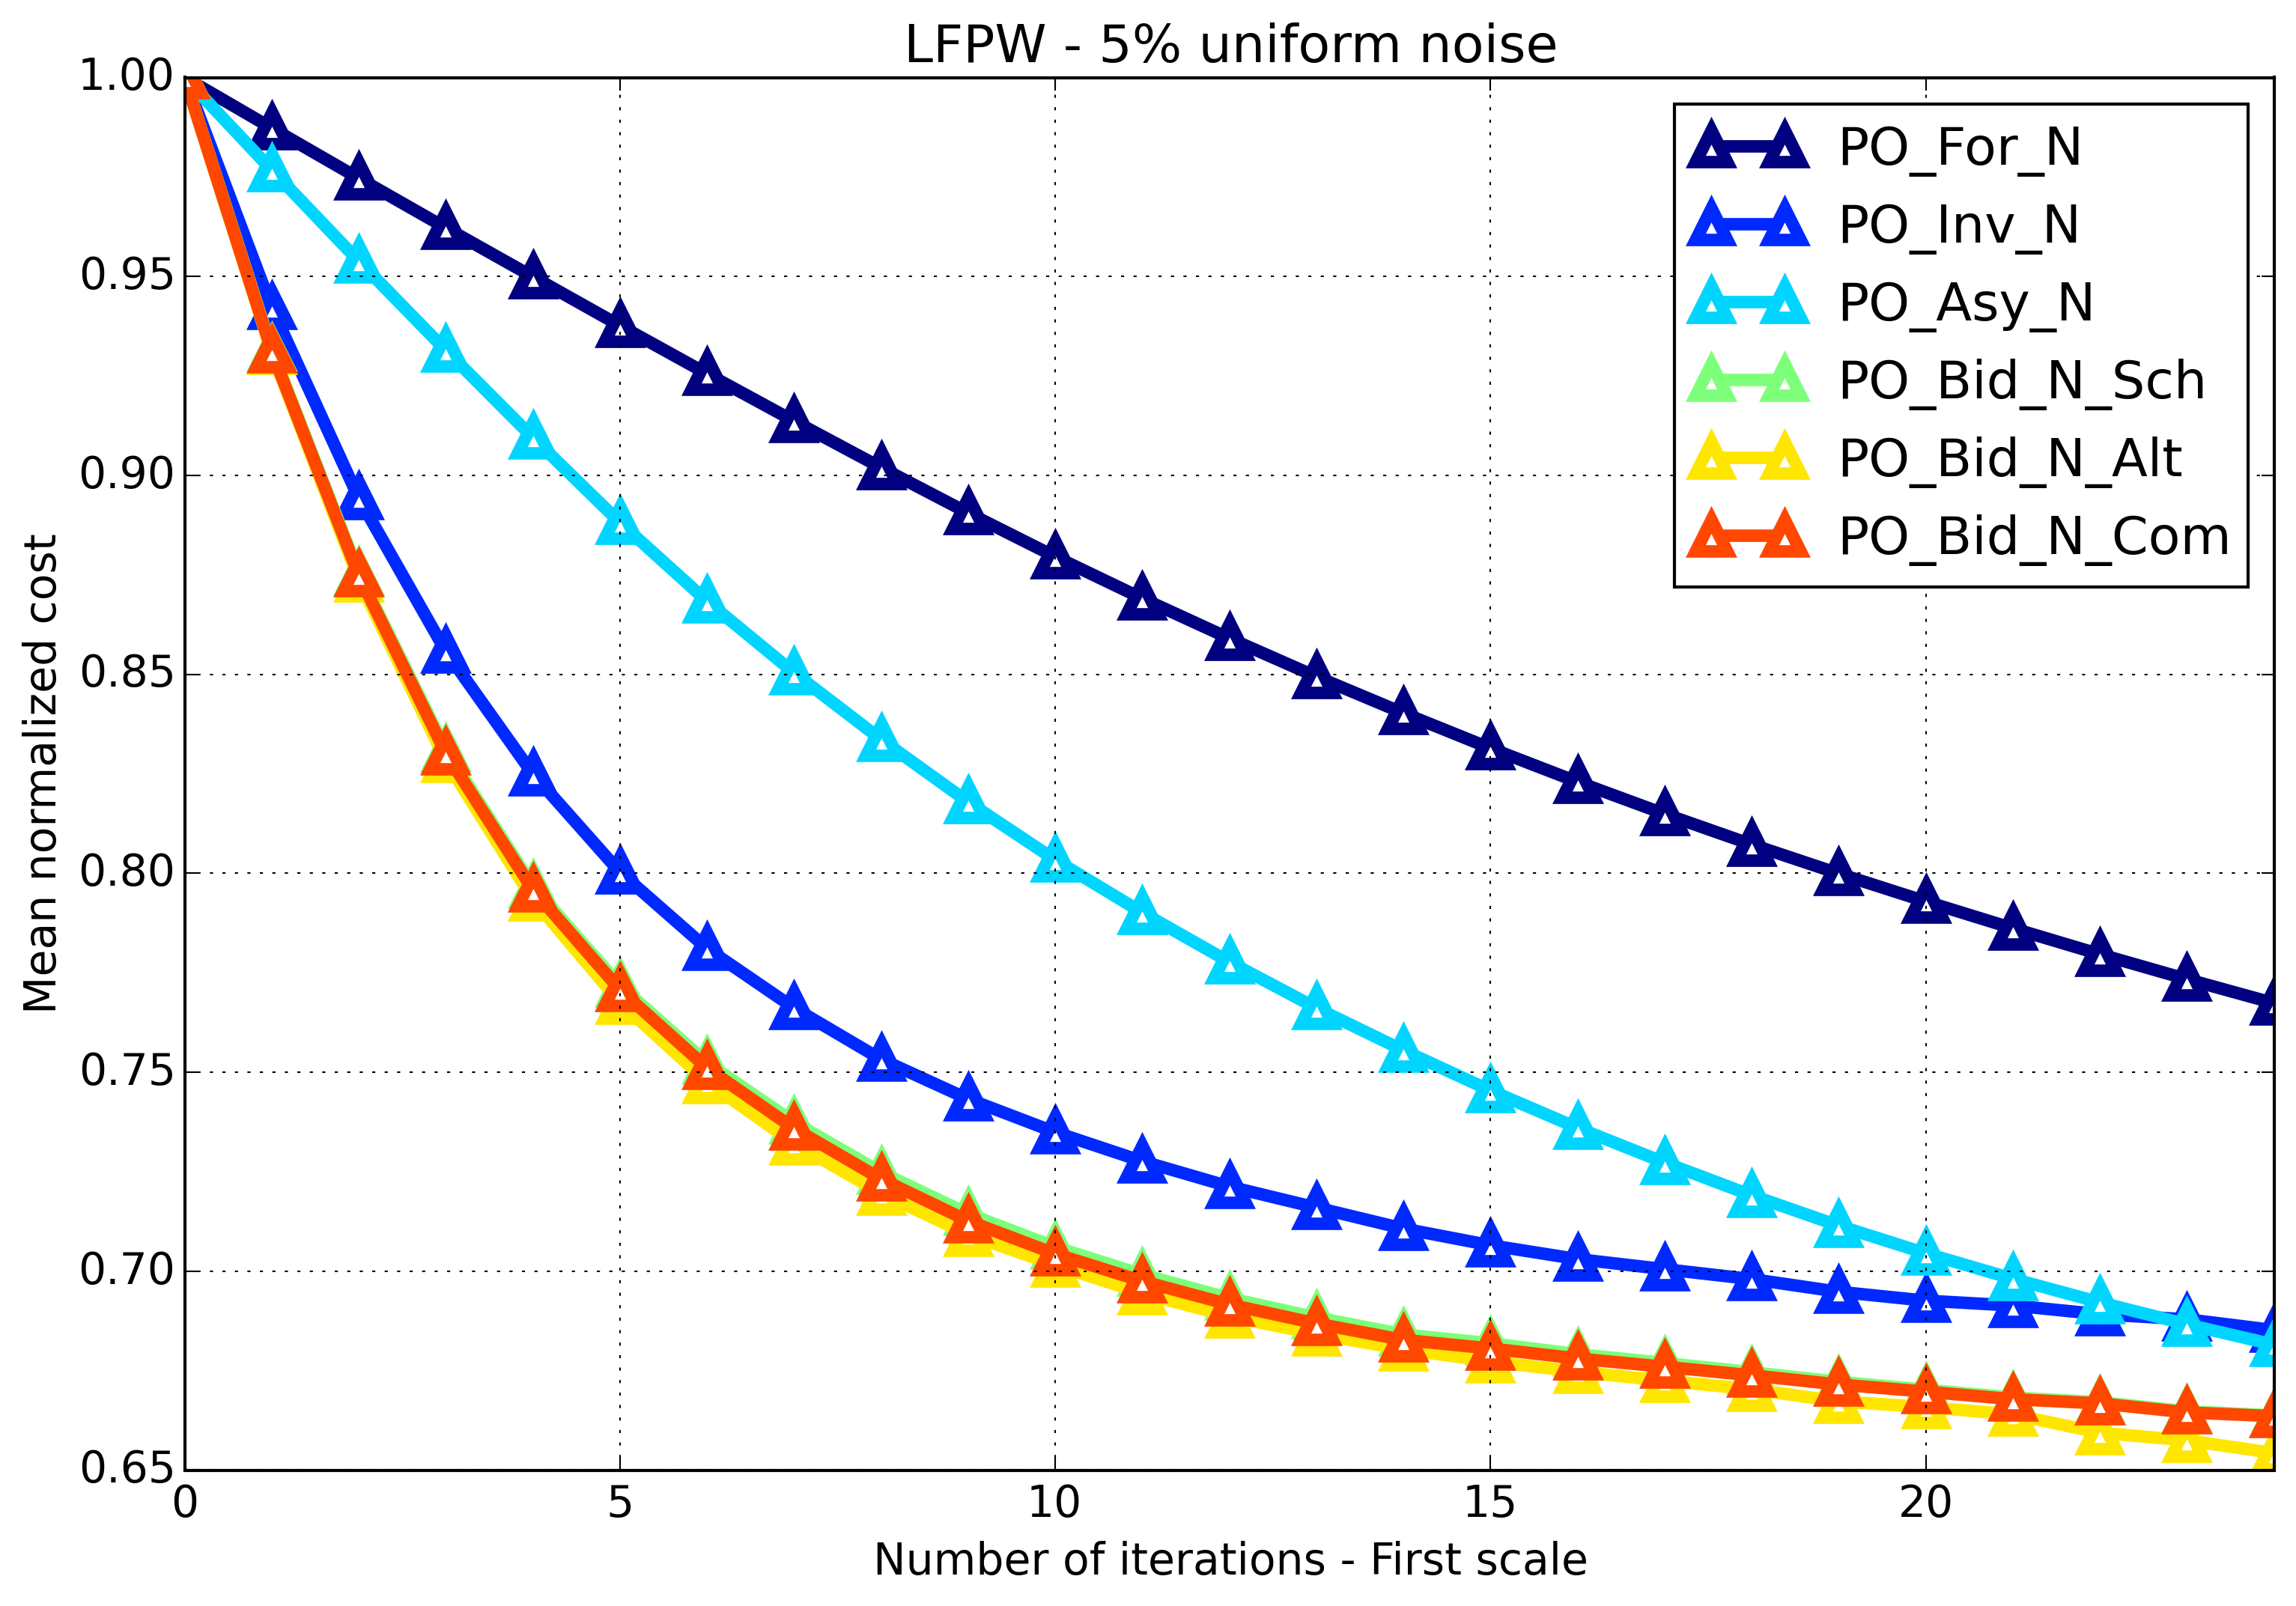
\includegraphics[width=0.50\textwidth]{experiments/algorithms/po_n/mean_cost_vs_iters1_po_n_5.png}
%     \caption{Mean normalized cost vs number of first scale iterations graph on the LFPW test dataset for all Project-Out Newton algorithms initialized with $4$\% uniform noise.}
%     \label{fig:mean_cost_vs_iters1_po_n_4}
% \end{figure}

% \begin{figure}[h!]
%     \centering
%     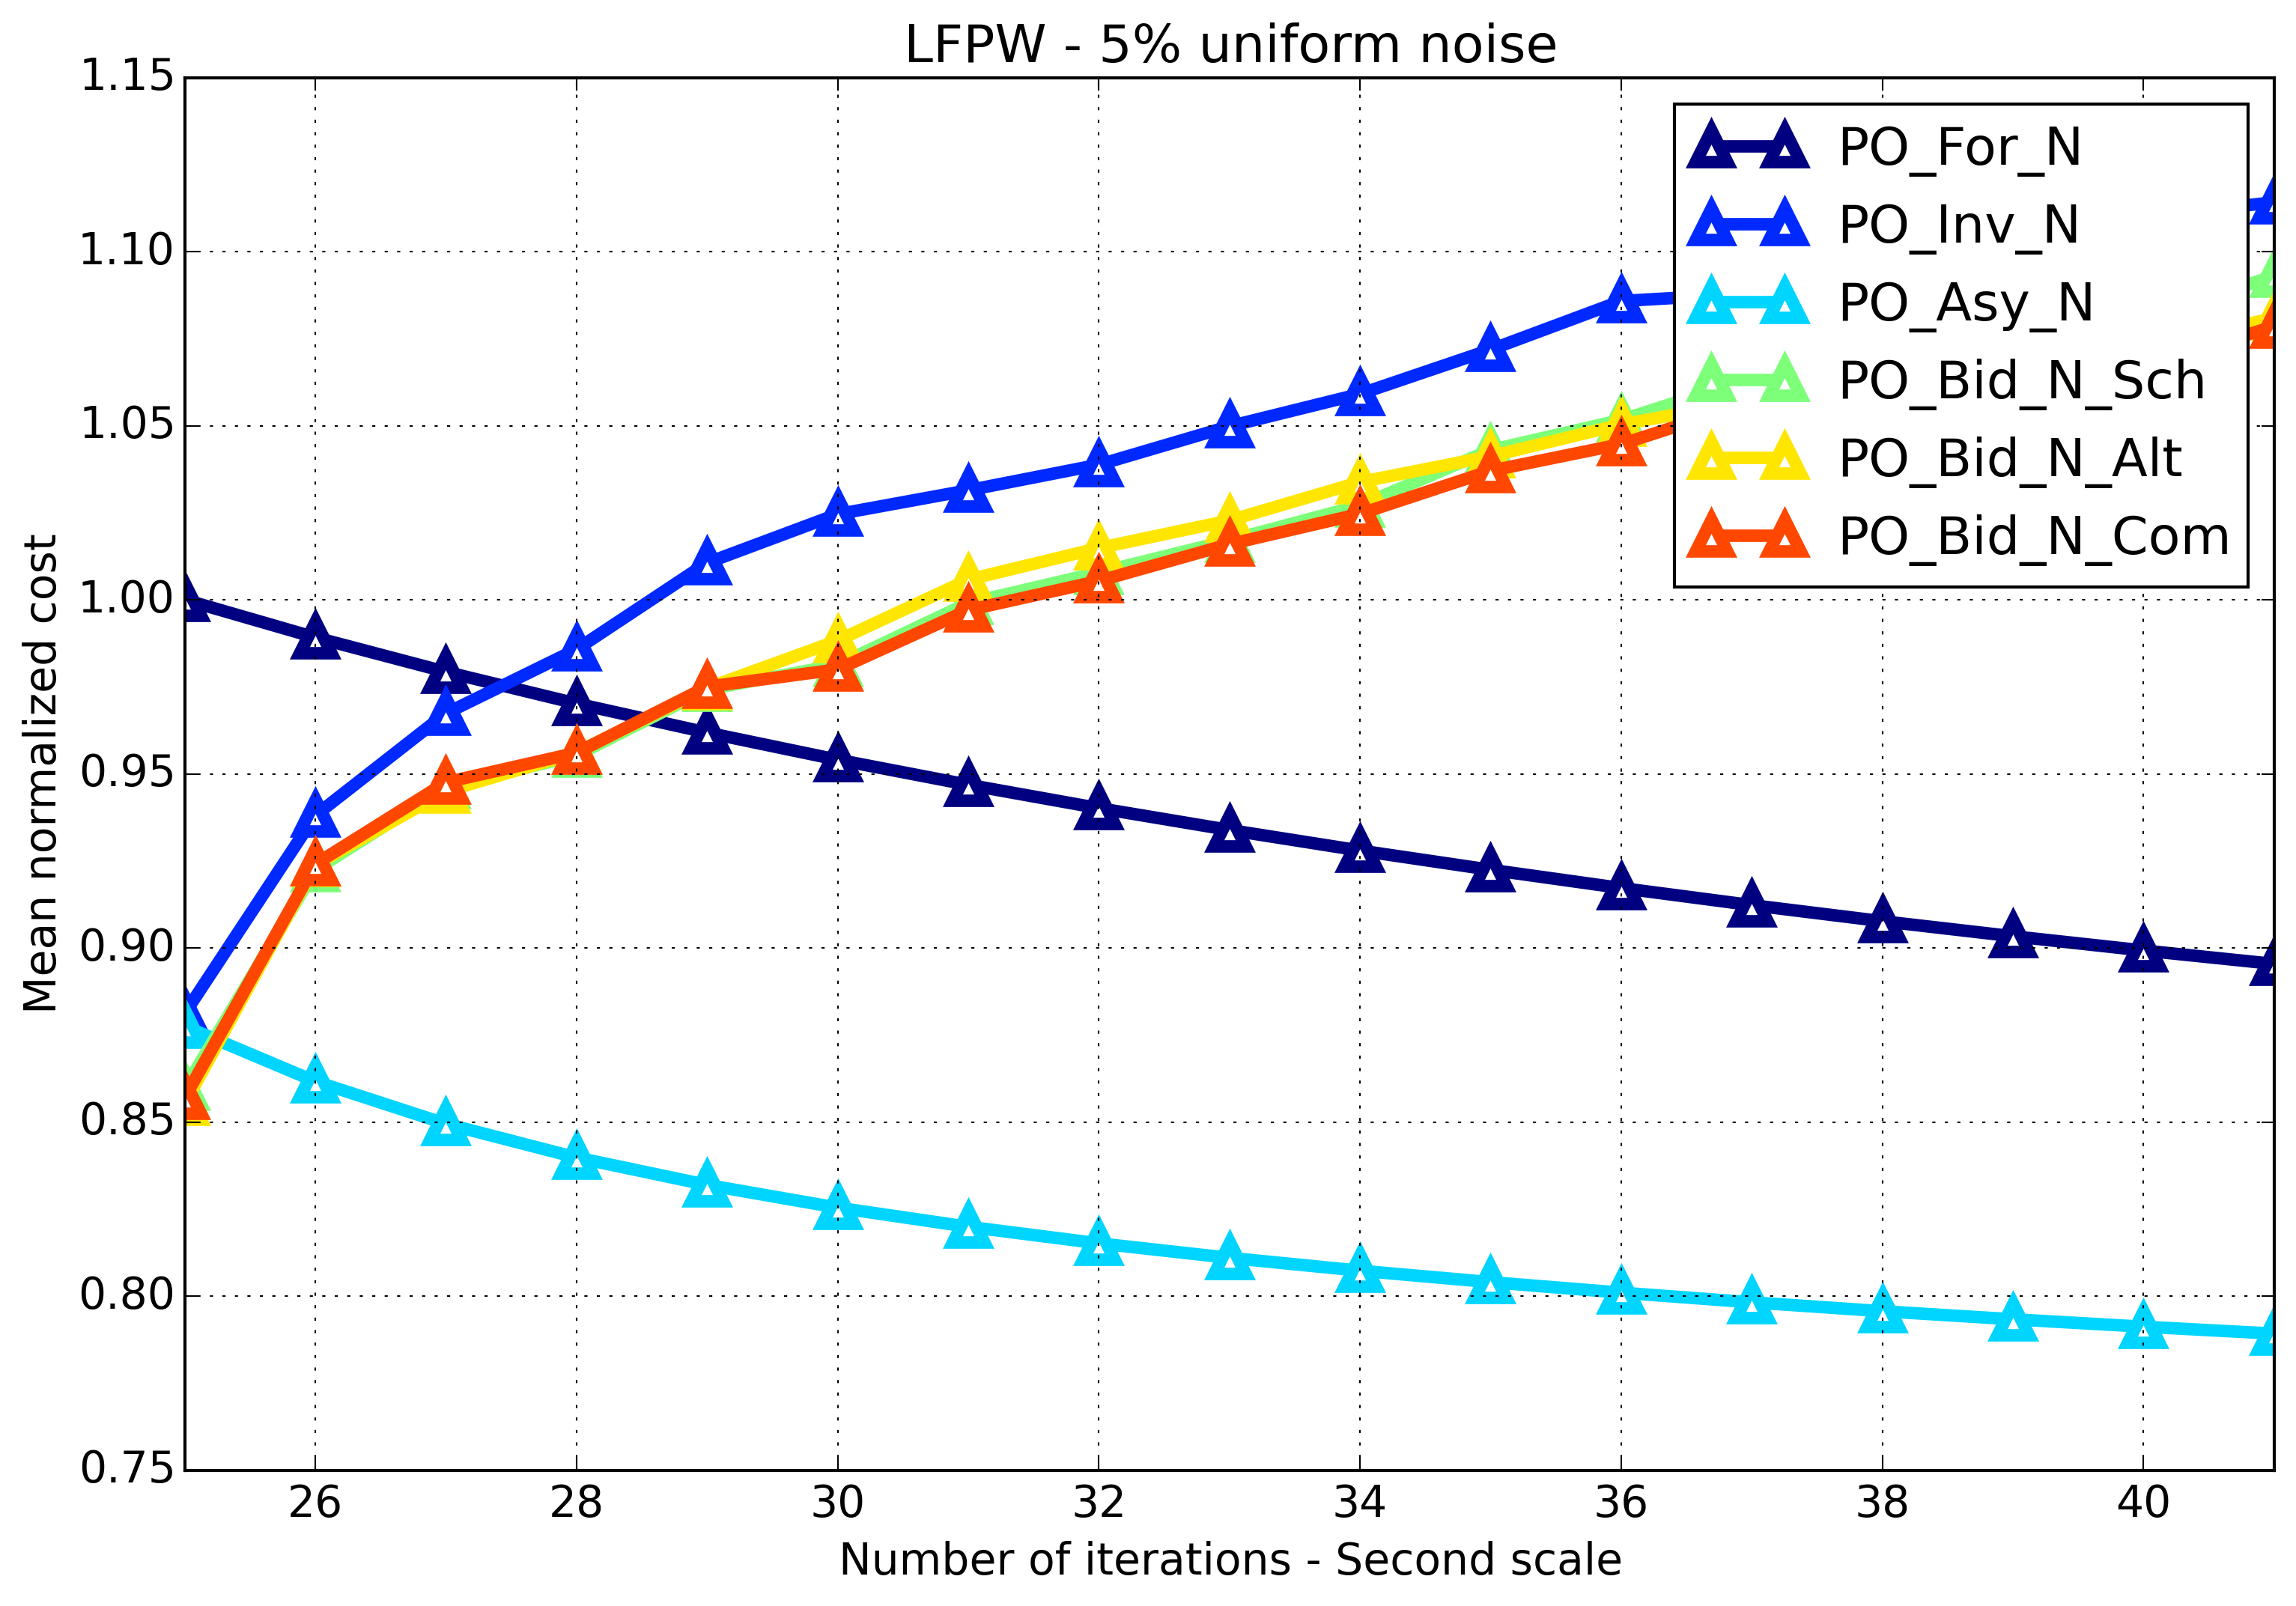
\includegraphics[width=0.50\textwidth]{experiments/algorithms/po_n/mean_cost_vs_iters2_po_n_5.png}
%     \caption{Mean normalized cost vs number of second scale iterations graph on the LFPW test dataset for all Project-Out Newton algorithms initialized with $4$\% uniform noise.}
%     \label{fig:mean_cost_vs_iters2_po_n_4}
% \end{figure}

\subsubsection*{Wiberg}

\begin{figure*}[h!]
	\centering
	\begin{subfigure}{0.48\textwidth}
	    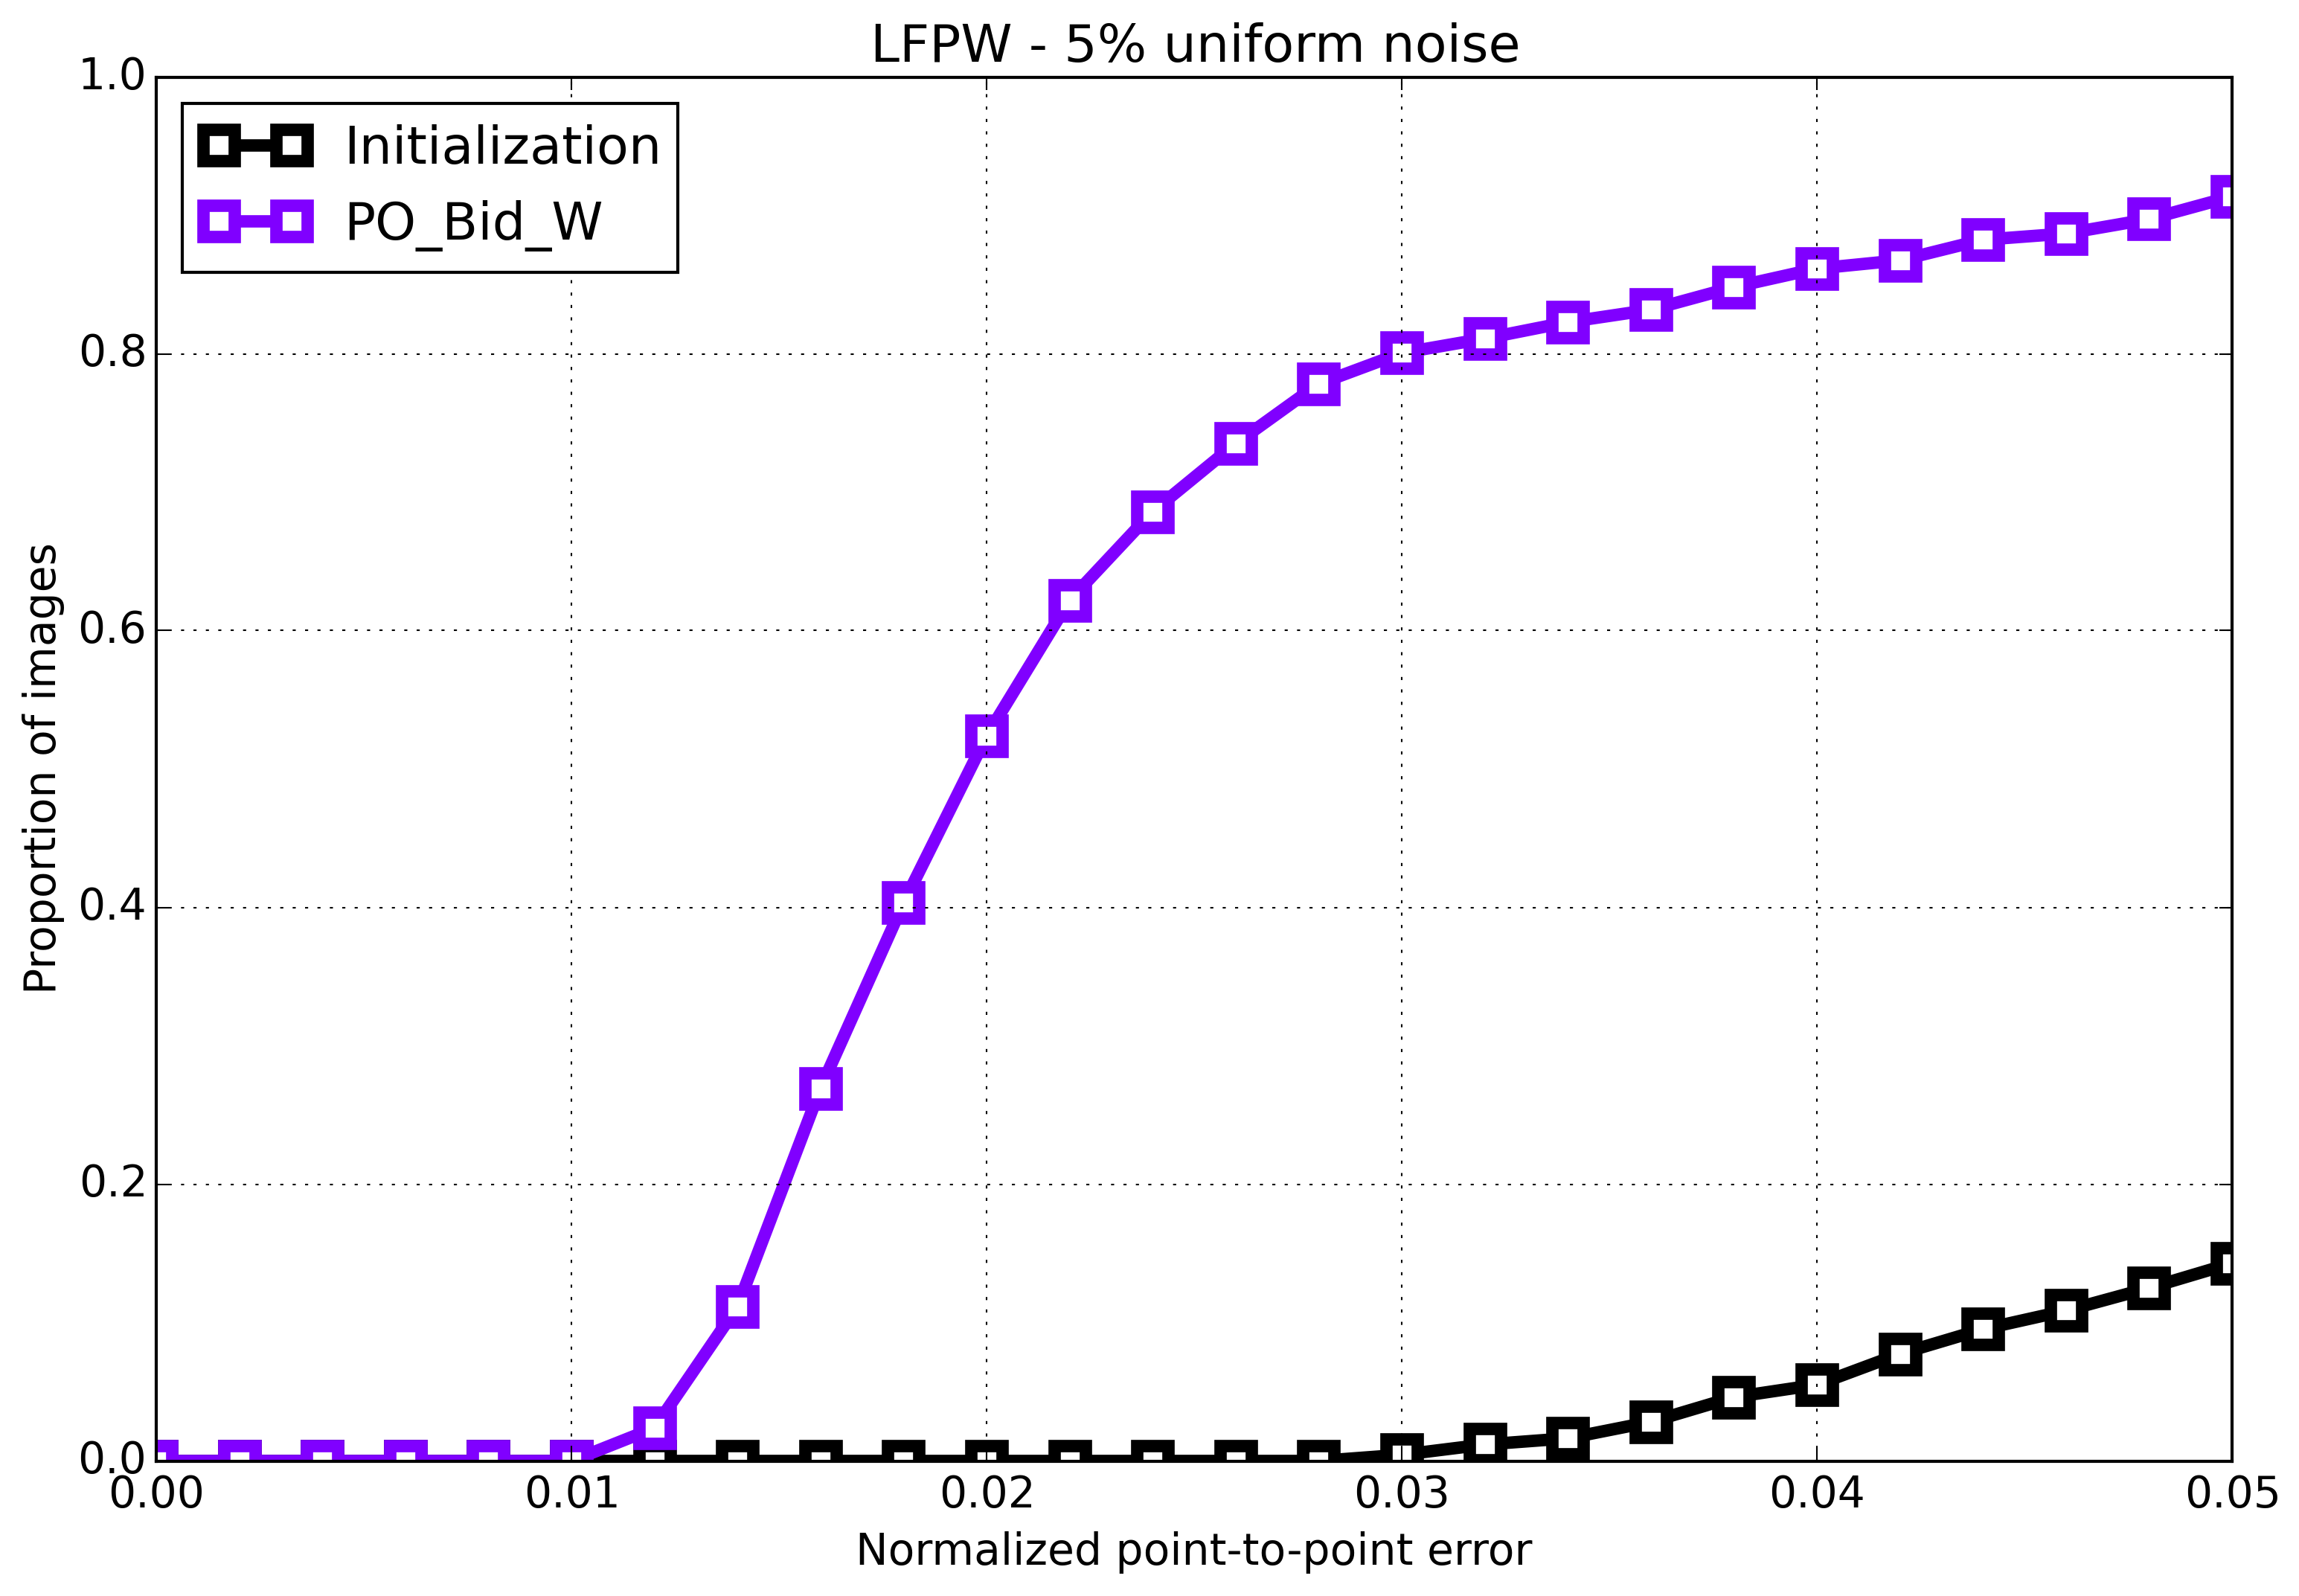
\includegraphics[width=\textwidth]{experiments/algorithms/po_w/ced_po_w_5.png}
	    \caption{Cumulative Error Distribution graph on the LFPW test dataset for all Project-Out Wiberg algorithms initialized with $5\%$ uniform noise.}
	    \label{fig:ced_po_w_5}
	\end{subfigure}
	\hfill
	\begin{subfigure}{0.48\textwidth}
	    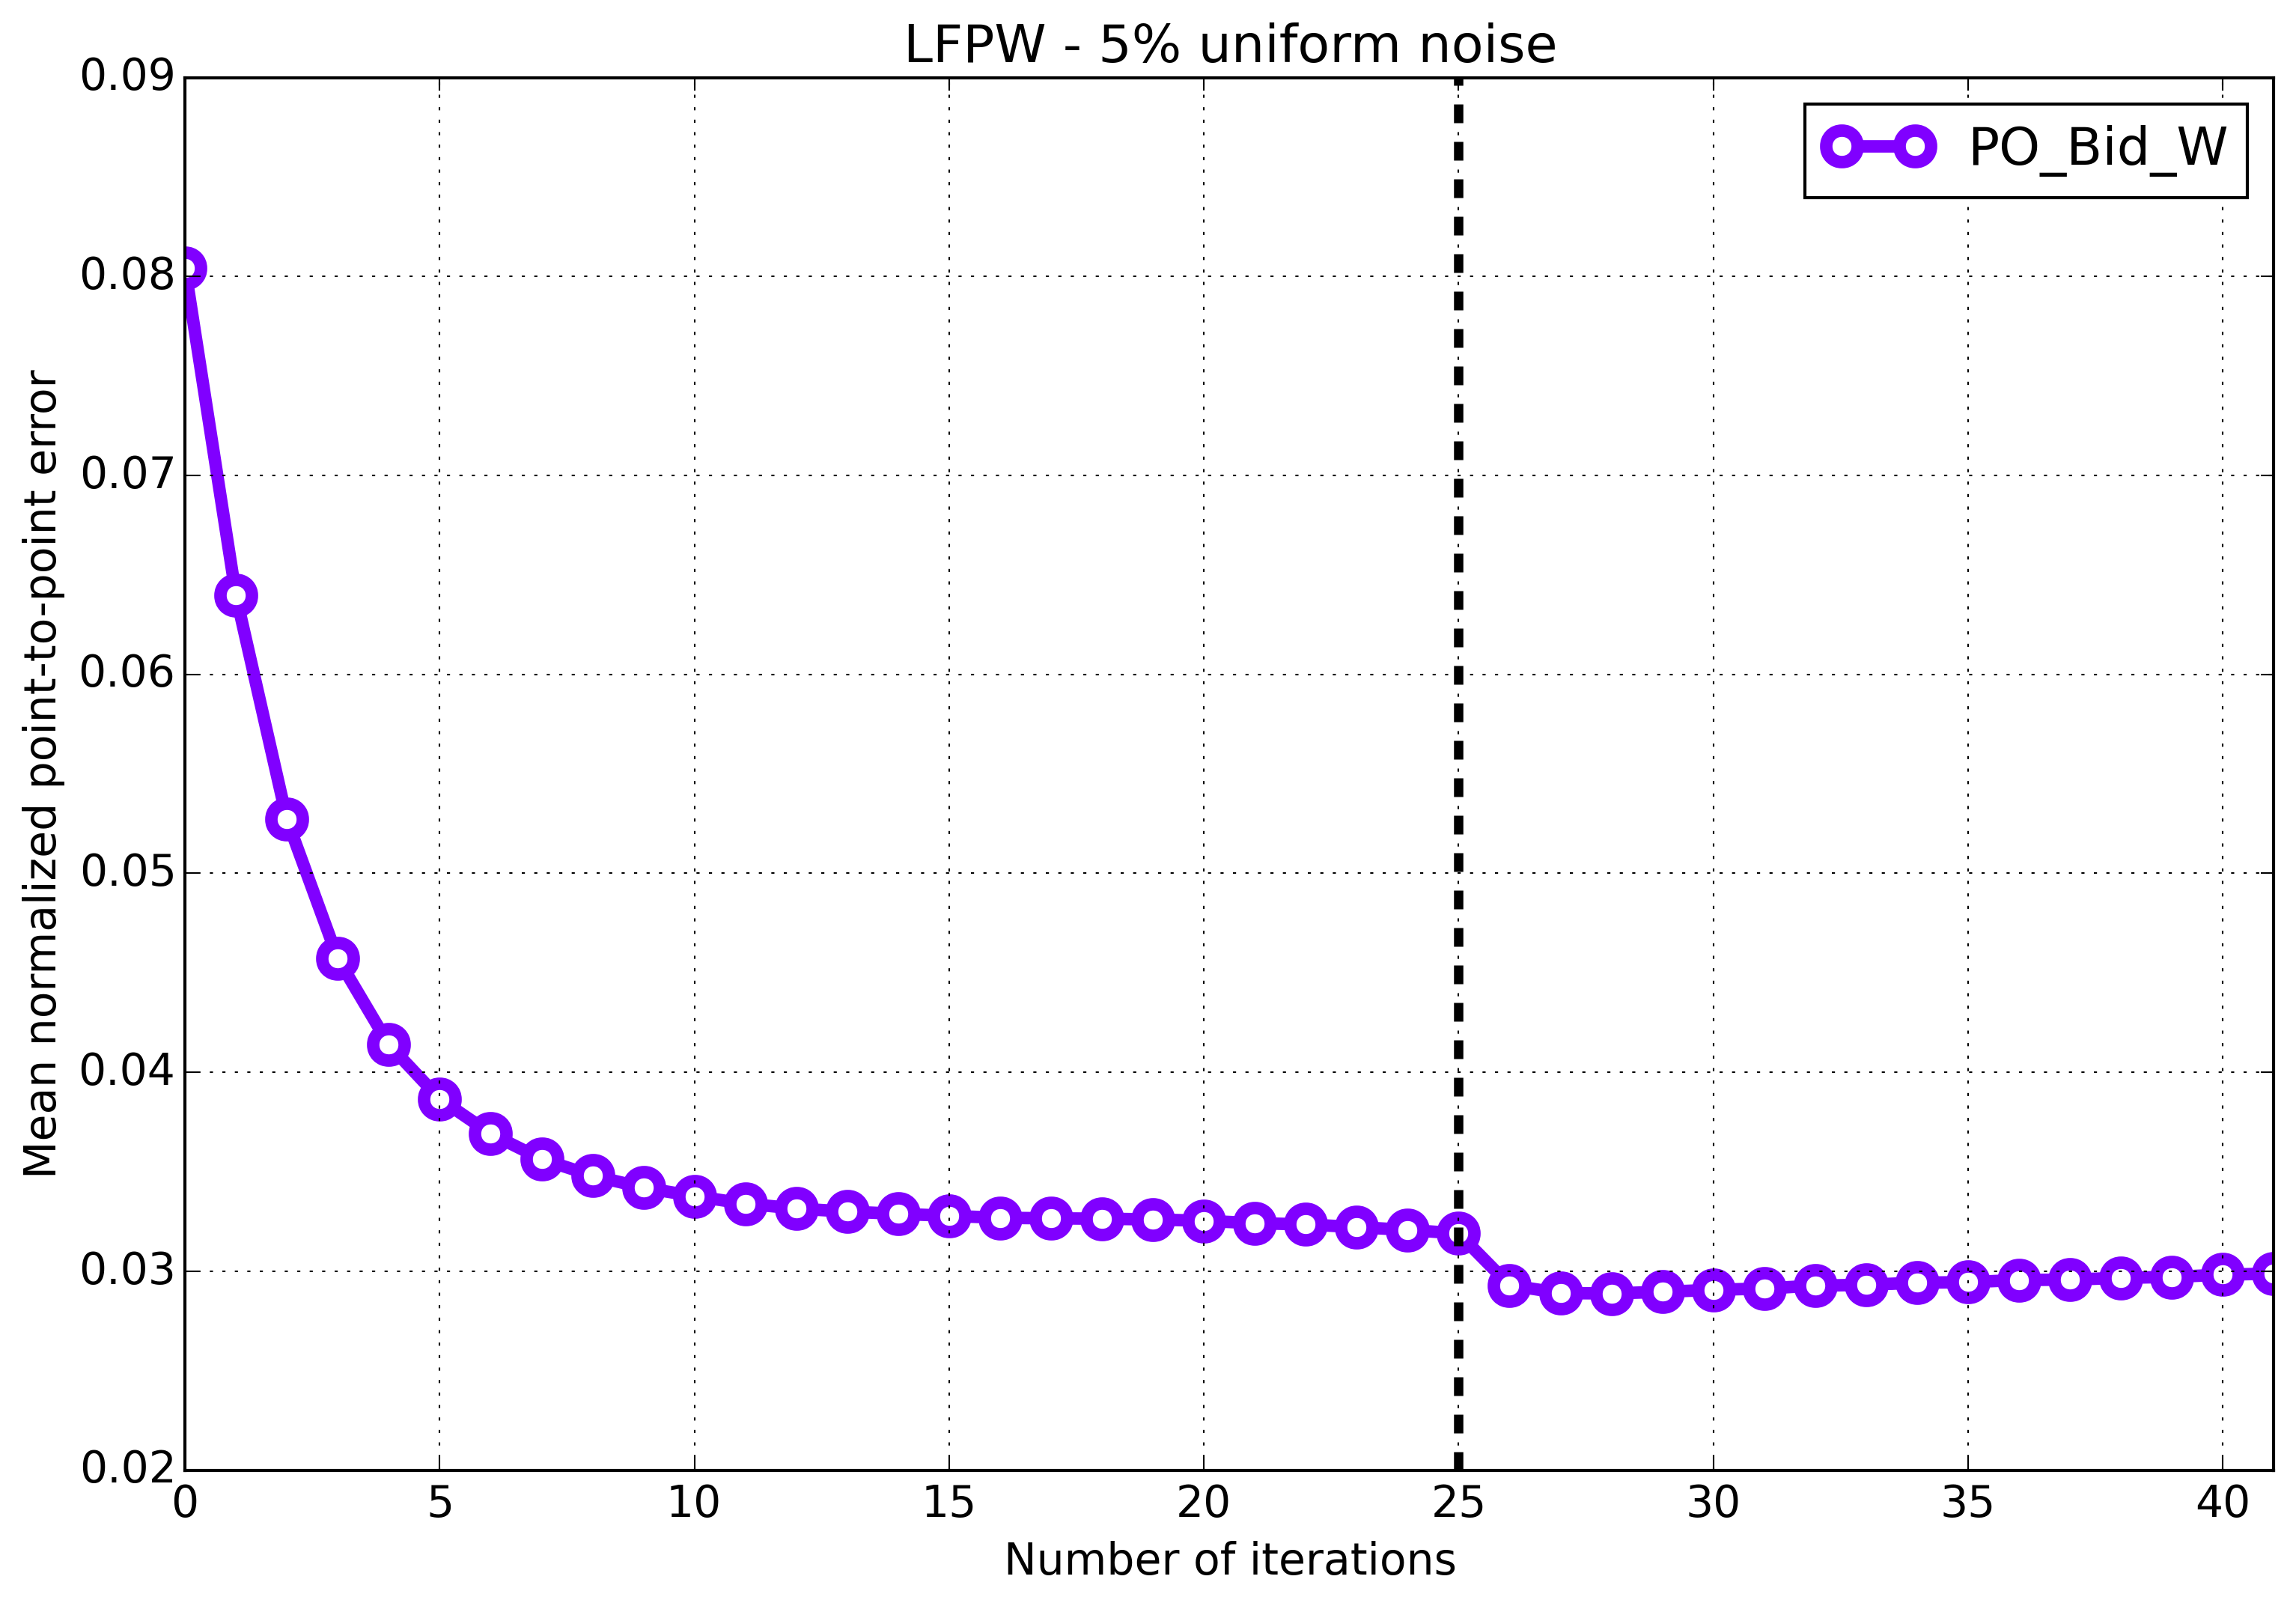
\includegraphics[width=\textwidth]{experiments/algorithms/po_w/mean_error_vs_iters_po_w_5.png}
	    \caption{Mean normalized point-to-point error vs number of iterations graph on the LFPW test dataset for all Project-Out Wiberg algorithms initialized with $5\%$ uniform noise.}
	    \label{fig:mean_error_vs_iters_po_w_5}
	\end{subfigure}
	\par\medskip
	\begin{subfigure}{0.48\textwidth}
	    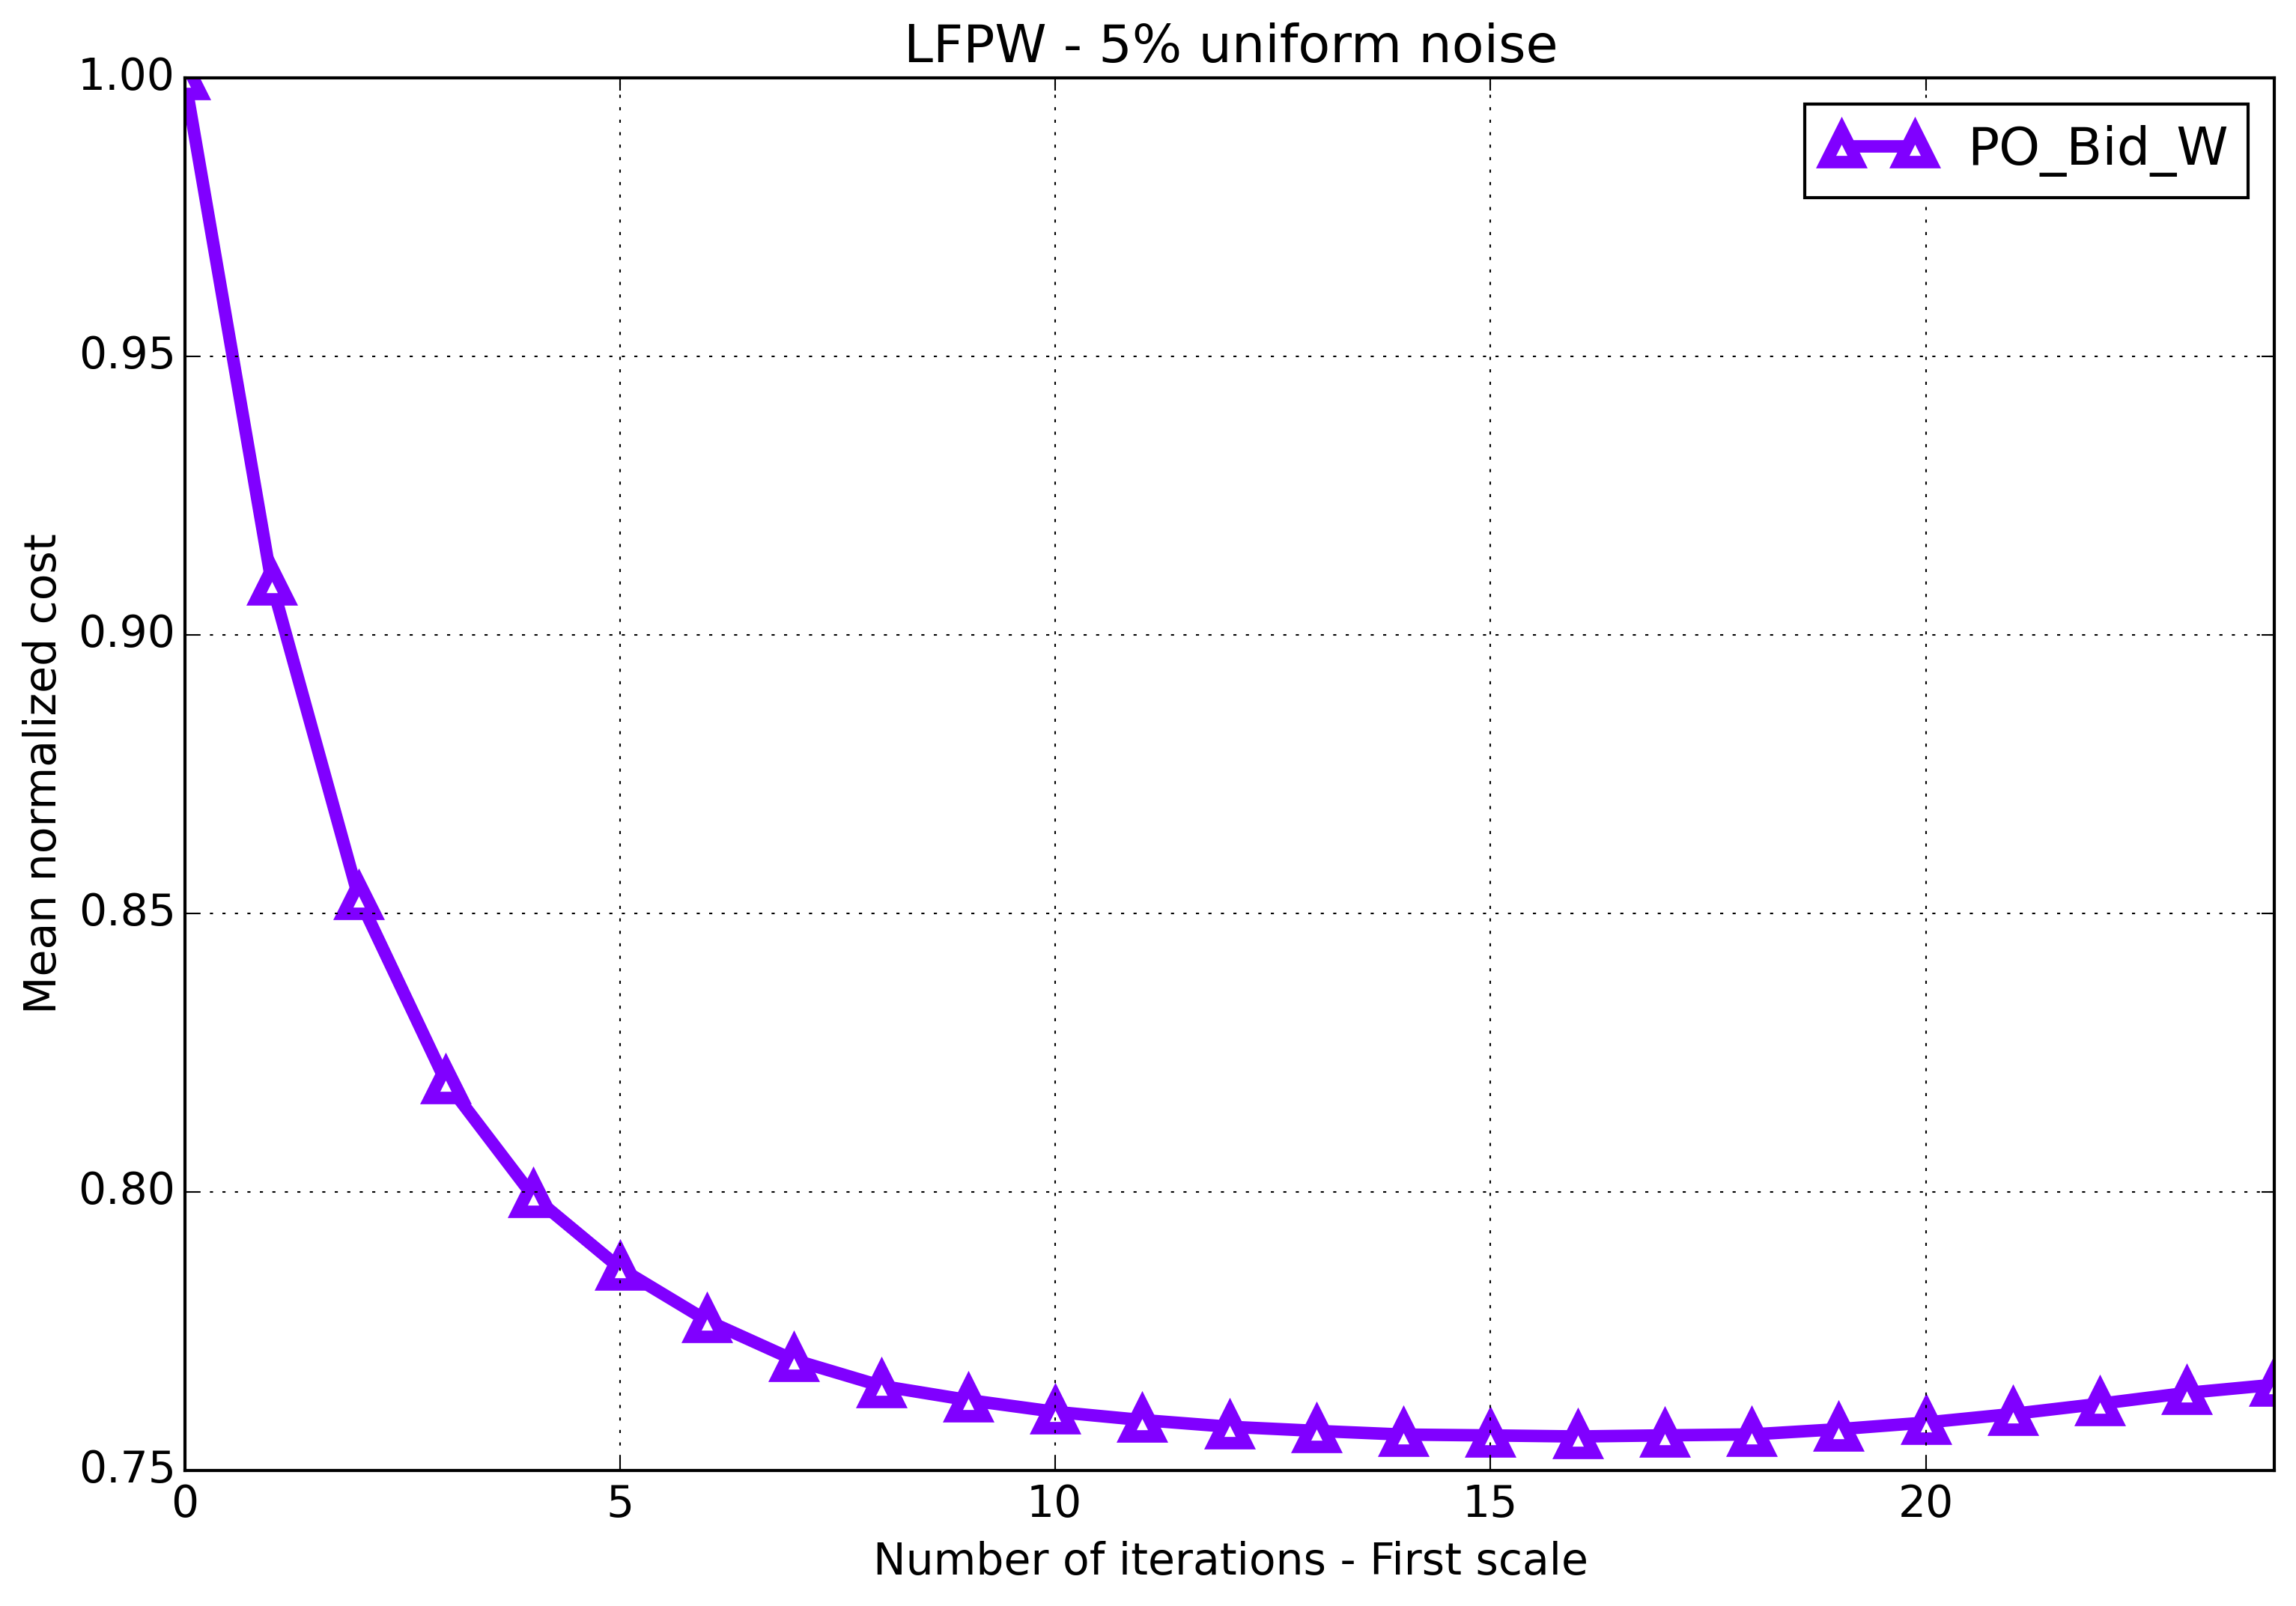
\includegraphics[width=\textwidth]{experiments/algorithms/po_w/mean_cost_vs_iters1_po_w_5.png}
	    \caption{Mean normalized cost vs number of first scale iterations graph on the LFPW test dataset for all Project-Out Wiberg algorithms initialized with $5\%$ uniform noise.}
	    \label{fig:mean_cost_vs_iters1_po_w_5}
	\end{subfigure}
	\hfill
	\begin{subfigure}{0.48\textwidth}
	    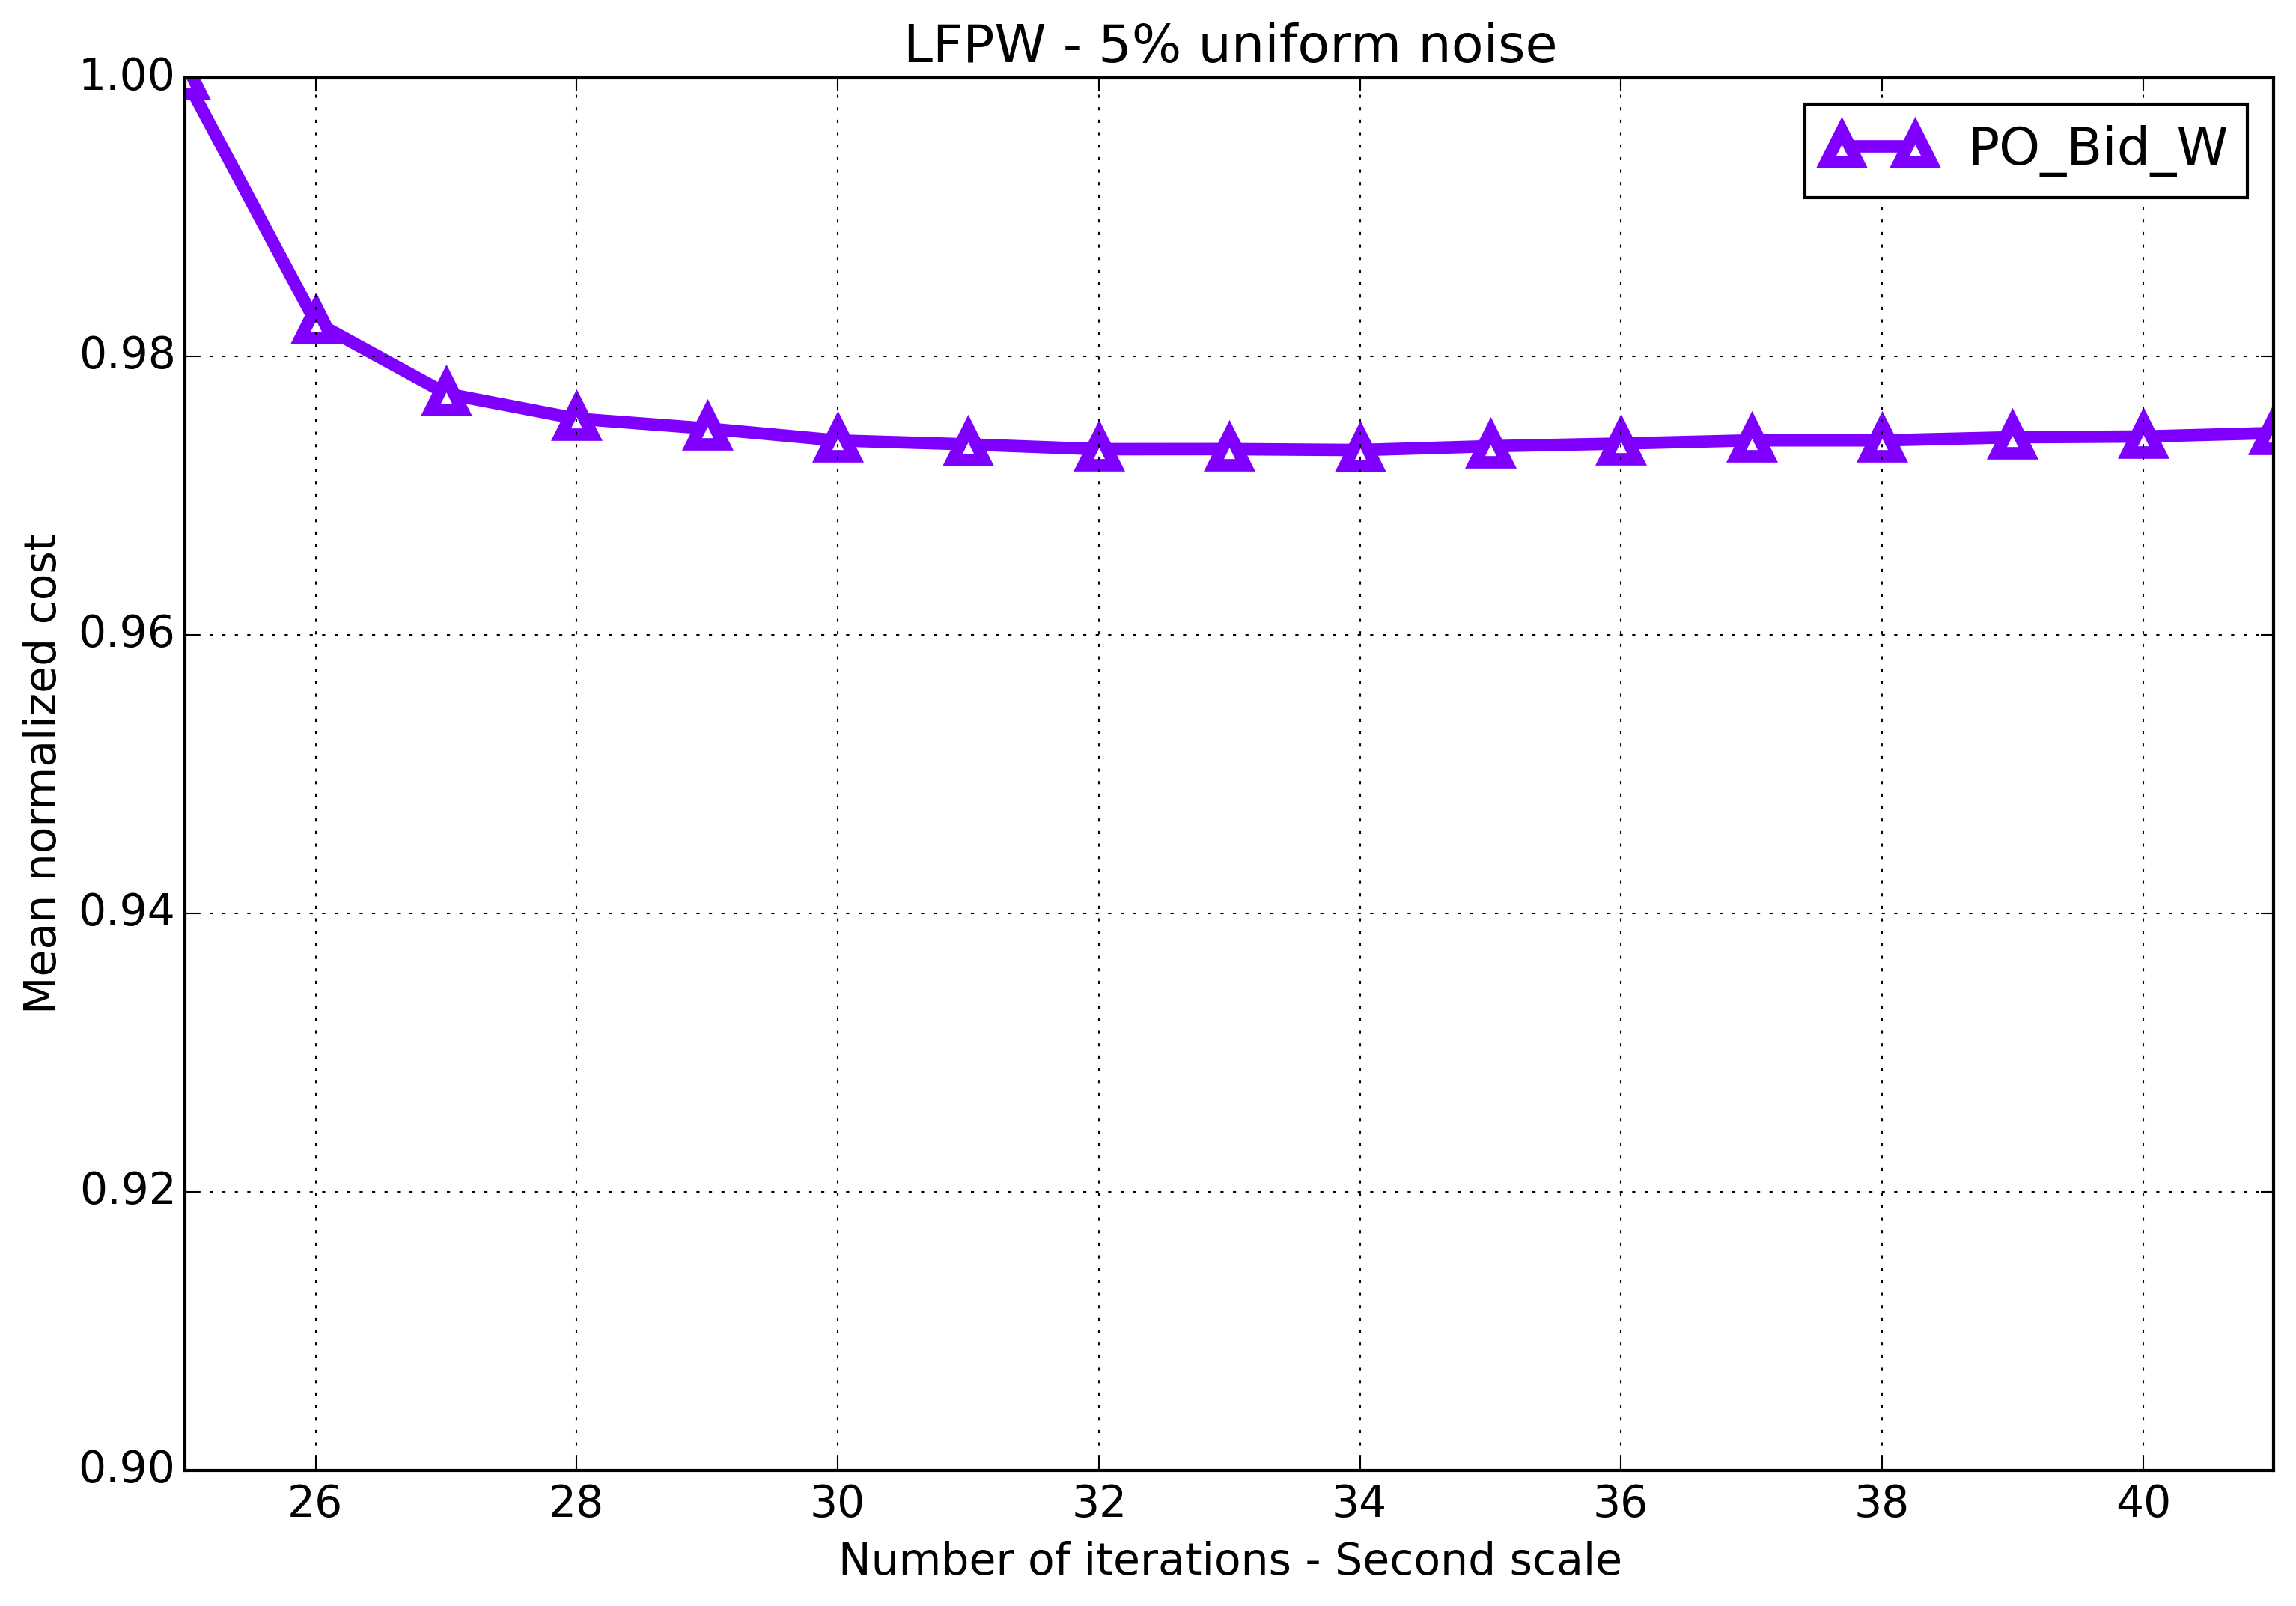
\includegraphics[width=\textwidth]{experiments/algorithms/po_w/mean_cost_vs_iters2_po_w_5.png}
	    \caption{Mean normalized cost vs number of second scale iterations graph on the LFPW test dataset for all Project-Out Wiberg algorithms initialized with $5\%$ uniform noise.}
	    \label{fig:mean_cost_vs_iters2_po_w_5}
	\end{subfigure}
	\label{fig:po_w_5}
	\caption{}
\end{figure*}


% \begin{figure}[h!]
%     \centering
%     \includegraphics[width=0.50\textwidth]{experiments/algorithms/ssd_gn/ced_ssd_gn_4.png}
%     \caption{CED graph on the LFPW test dataset for all SSD Gauss-Newton algorithms initialized with $4$\% of uniform noise.}
%     \label{fig:ced_po_asymmetric_gn_4}
% \end{figure}




% \begin{figure}[h!]
%     \centering
%     \includegraphics[width=0.50\textwidth]{experiments/algorithms/ssd_gn/mean_error_vs_iters_ssd_gn_4.png}
%     \caption{Mean normalized point-to-point error vs number of iterations graph on the LFPW test dataset for all SSD Gauss-Newton algorithms initialized with $4$\% of uniform noise}
%     \label{fig:mean_error_vs_iters_po_asymmetric_gn_4}
% \end{figure}


\subsubsection{Weighted Bayesian project-out}

In this experiment, we quantify the importance of each of the two terms in our Bayesian project-out cost function, Equation \ref{eq:prob_po}. To this end, we introduce the parameters, $\rho \in [0, 1]$ and $\gamma = 1 - \rho$, to weight up the relative contribution of both terms as follows:
\begin{equation}
    \begin{aligned}
        \rho|| \mathbf{i}[\mathbf{p}] - \mathbf{\bar{a}} ||^2_{\mathbf{A}\mathbf{D}^{-1}\mathbf{A}^T} 
        + 
        \frac{\gamma}{\sigma^2}|| \mathbf{i}[\mathbf{p}] - \mathbf{\bar{a}} ||^2_{\bar{\mathbf{A}}}
    \end{aligned}
    \label{eq:weighted_po}
\end{equation}
Setting $\rho=0$, $\gamma=1$ reduces the previous cost function to the original project-out loss proposed in \cite{Matthews2004}; completely disregarding the contribution of the prior distribution over the appearance parameters i.e the Mahalanobis distance \emph{within} the appearance subspace. On the contrary, setting $\rho=1$, $\gamma=0$ reduces the cost function to the first term; completely disregarding the contribution of the project-out term i.e. the distance \emph{to} the appearance subspace. Finally setting $\rho=\gamma=0.5$ leads to the standard Bayesian project-out cost function proposed in Section \ref{sec:po_pi}.
 
In order to asses the impact that each term has on the fitting accuracy obtained by the previous project-out algorithm we repeat the experimental set up of the first experiment and test all project-out algorithms for different values of the parameters $\rho$ and $\gamma$. Results for this experiment are reported by Figure \ref{fig:rho}. We can see that, regardless of the type of composition, a weighted combinations of the two previous terms always leads to a smaller mean normalized point-to-point error compared to either term on its own. Note that the accuracy achieved by the standard Bayesian project-out cost function is substantially better than the one obtained by the original project-out loss (specially noticeable for the inverse and bidirectional cases); fully justifying the inclusion of the first term, i.e the Mahalanobis distance \emph{within} the appearance subspace, into the cost function. Finally, in this particular experiment, the accuracy of all algorithms is maximized by setting $\rho=0.1$, $\gamma=0.9$, further highlighting the importance of the first term in the Bayesian formulation.

\begin{figure*}[h!]
	\centering
	\begin{subfigure}{\textwidth}
	    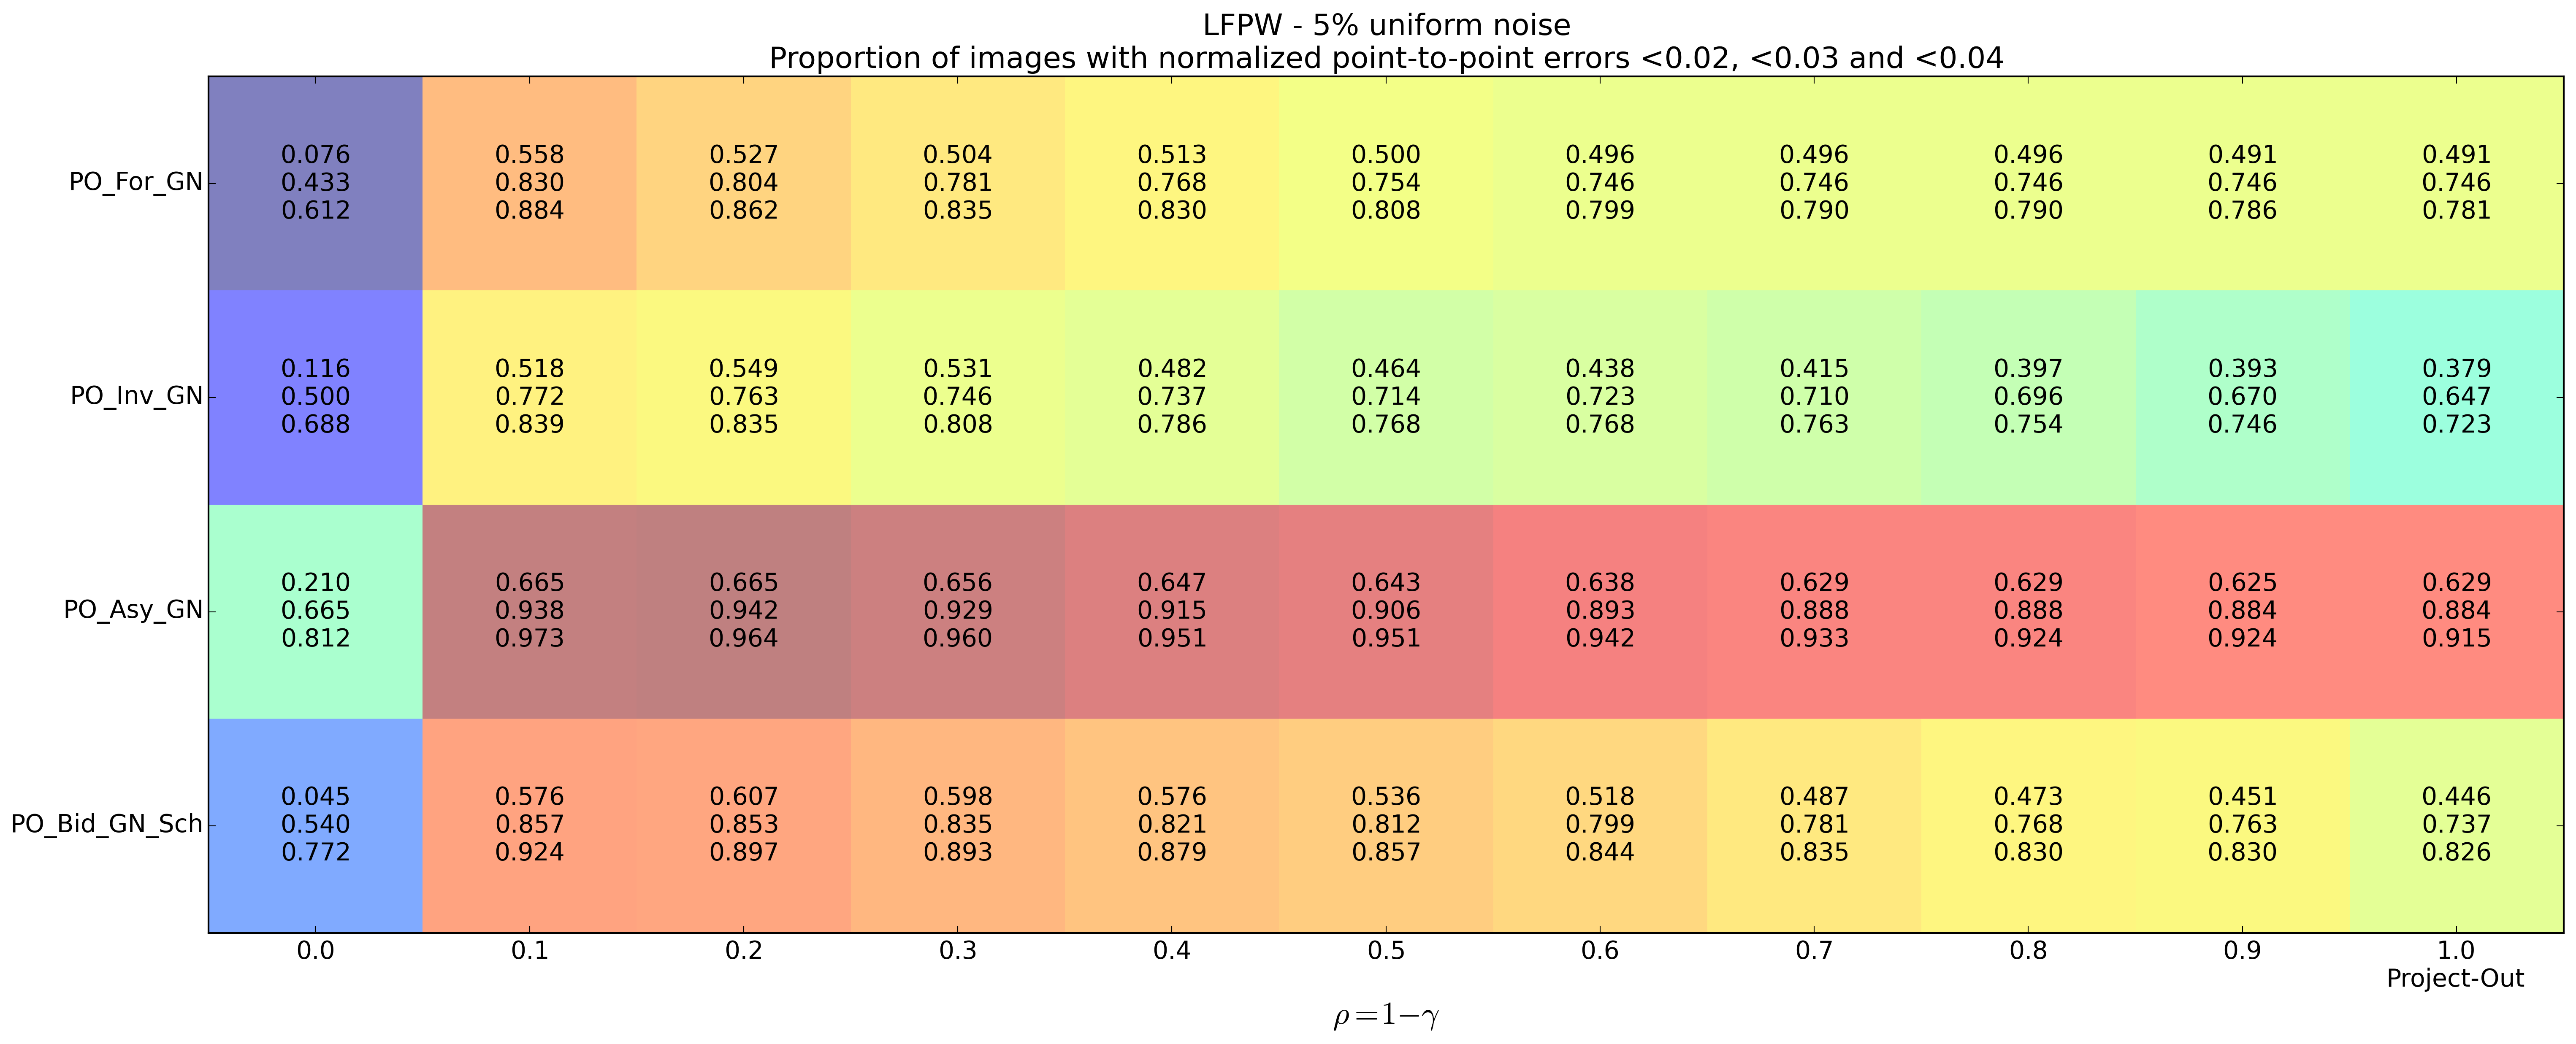
\includegraphics[width=\textwidth]{experiments/rho/convergence_vs_rho_po_gn_5.png}
	    \caption{Proportion of images with normalized point-to-point errors smaller than $0.02$, $0.03$ and $0.04$ for the Project-Out and SSD Asymmetric Gauss-Newton algorithms values of $\rho$ and $\gamma$ and initialized with $5\%$ noise.}
	    \label{fig:convergence_vs_rho_po_gn}
	\end{subfigure}
	\par\medskip
	\begin{subfigure}{0.48\textwidth}
	    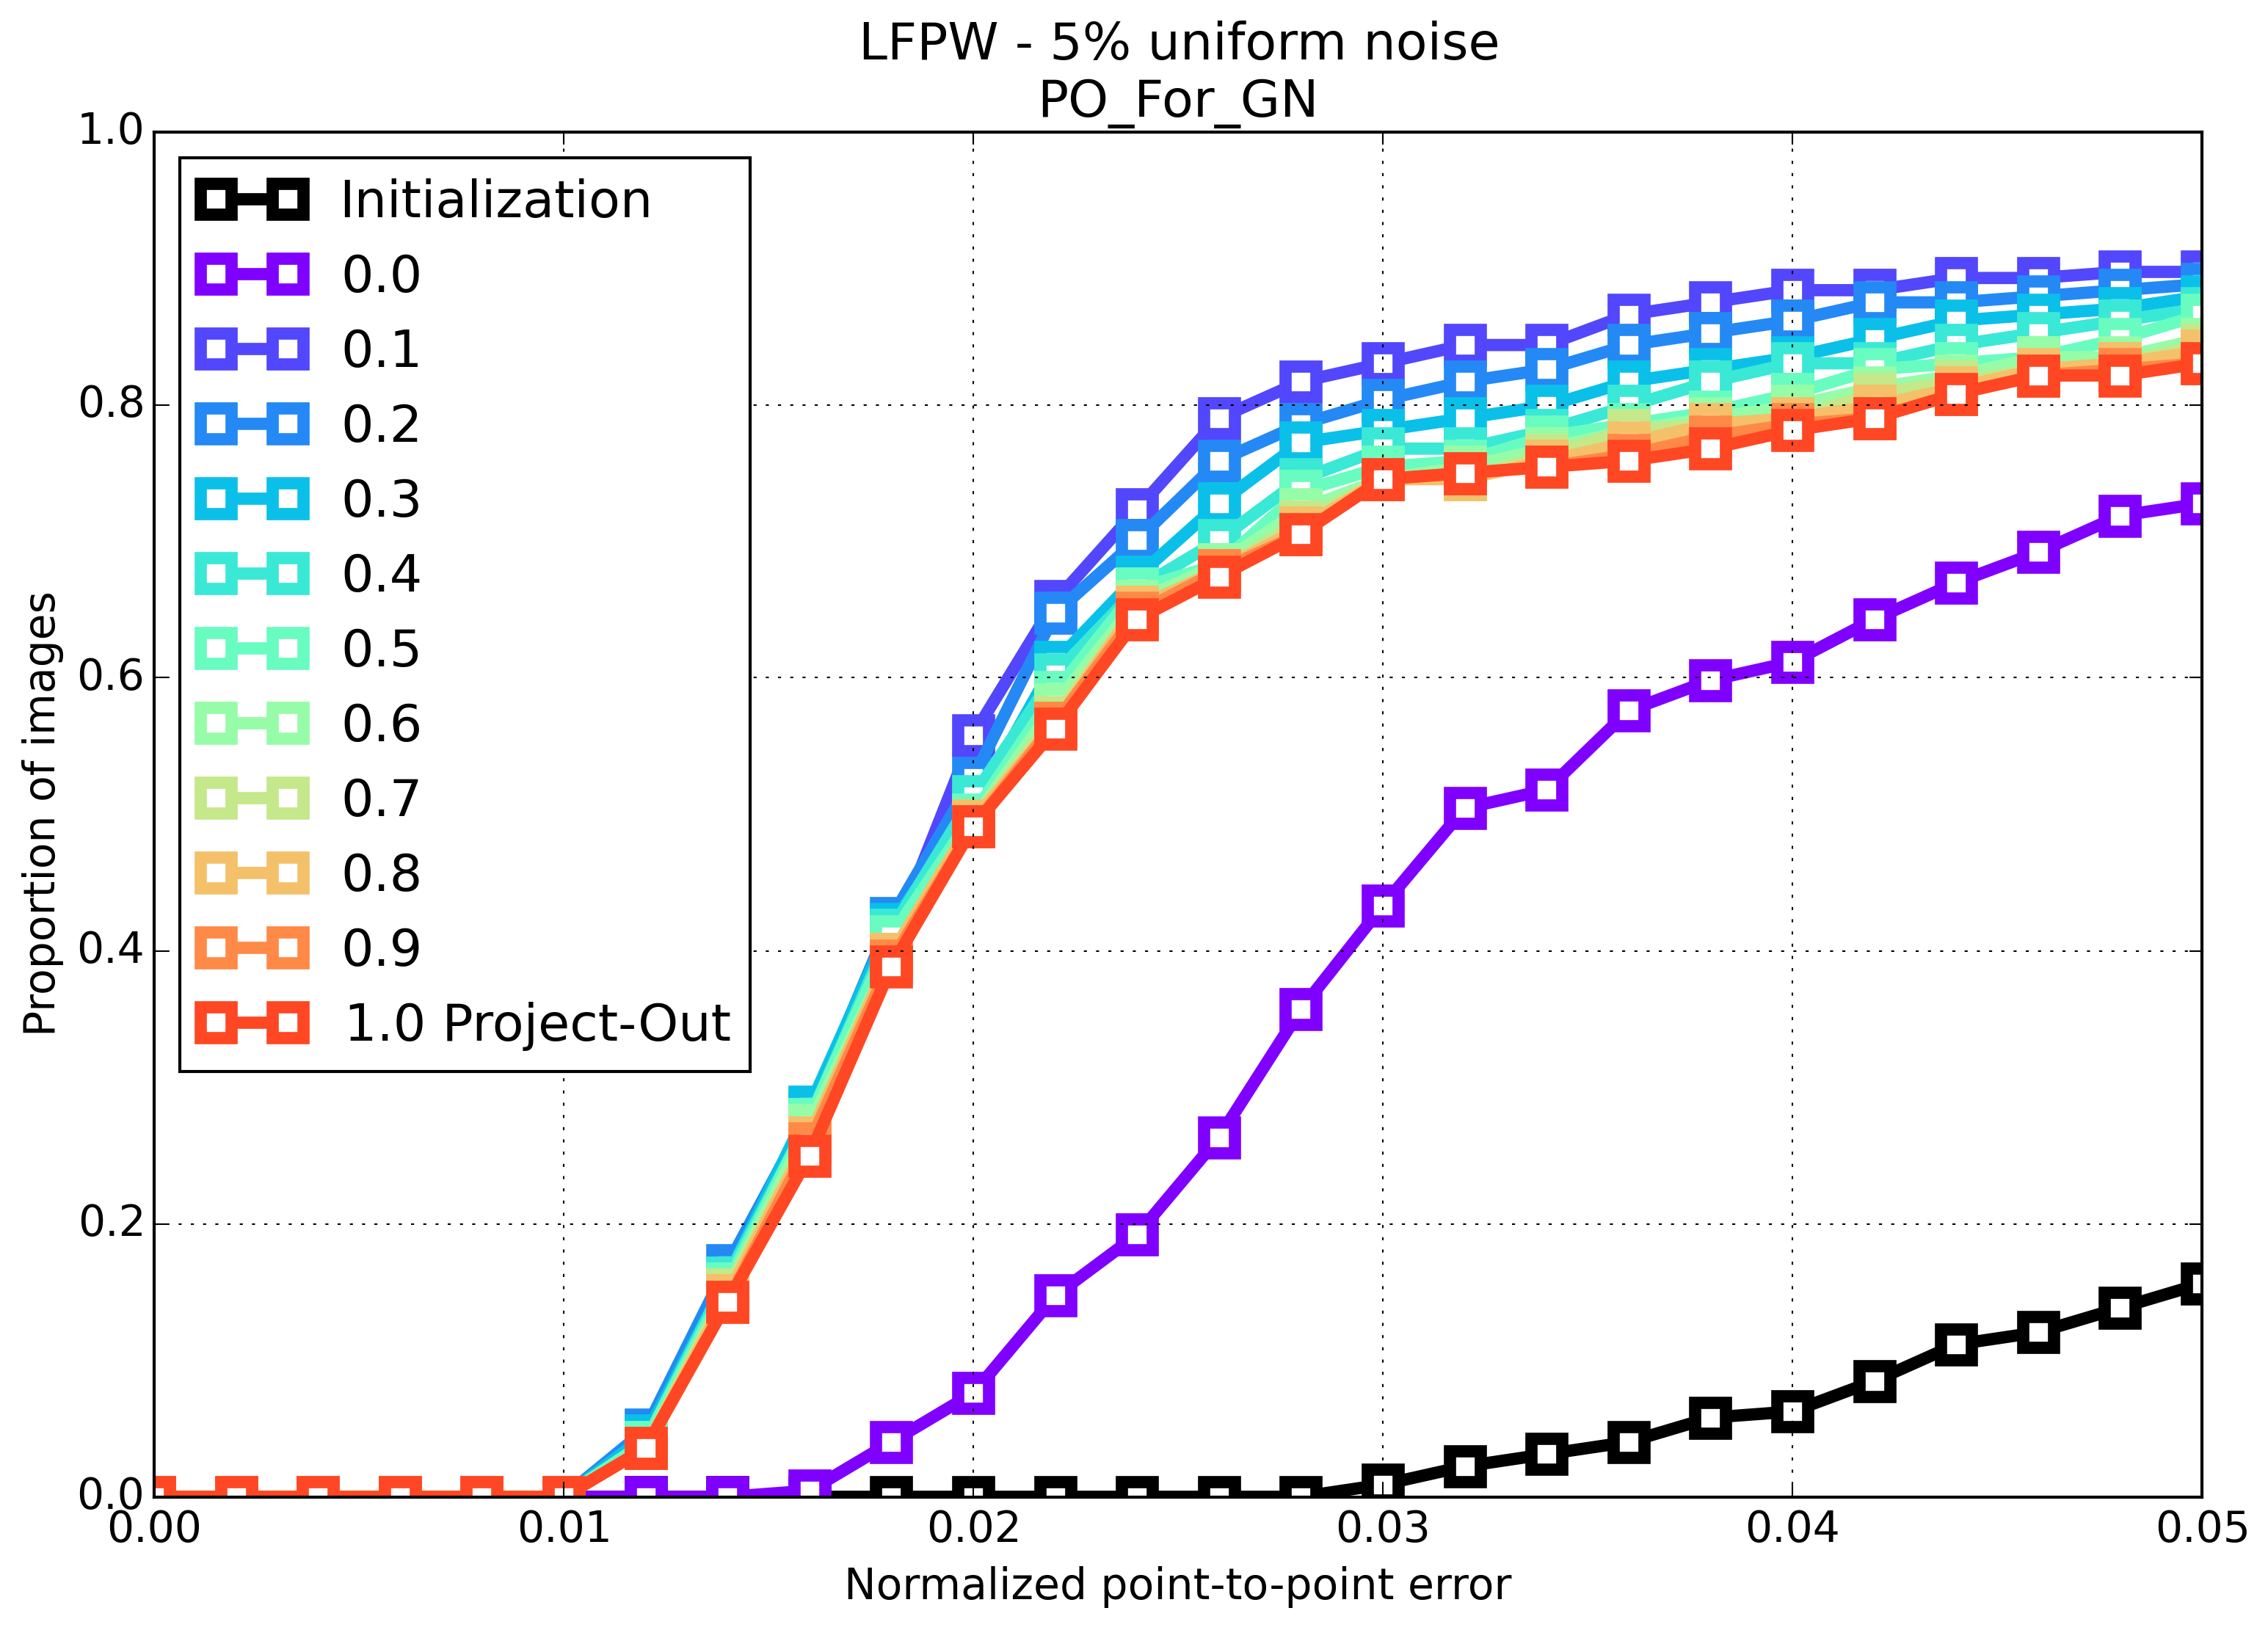
\includegraphics[width=\textwidth]{experiments/rho/ced_po_for_gn_5.png}
	    \caption{CED on the LFPW test dataset for Project-Out Forward Gauss-Newton algorithms for different values of $\rho$ and $\gamma$ and initialized with $5\%$ noise.}
	    \label{fig:ced_po_for_gn}
	\end{subfigure}
	\hfill
	\begin{subfigure}{0.48\textwidth}
	    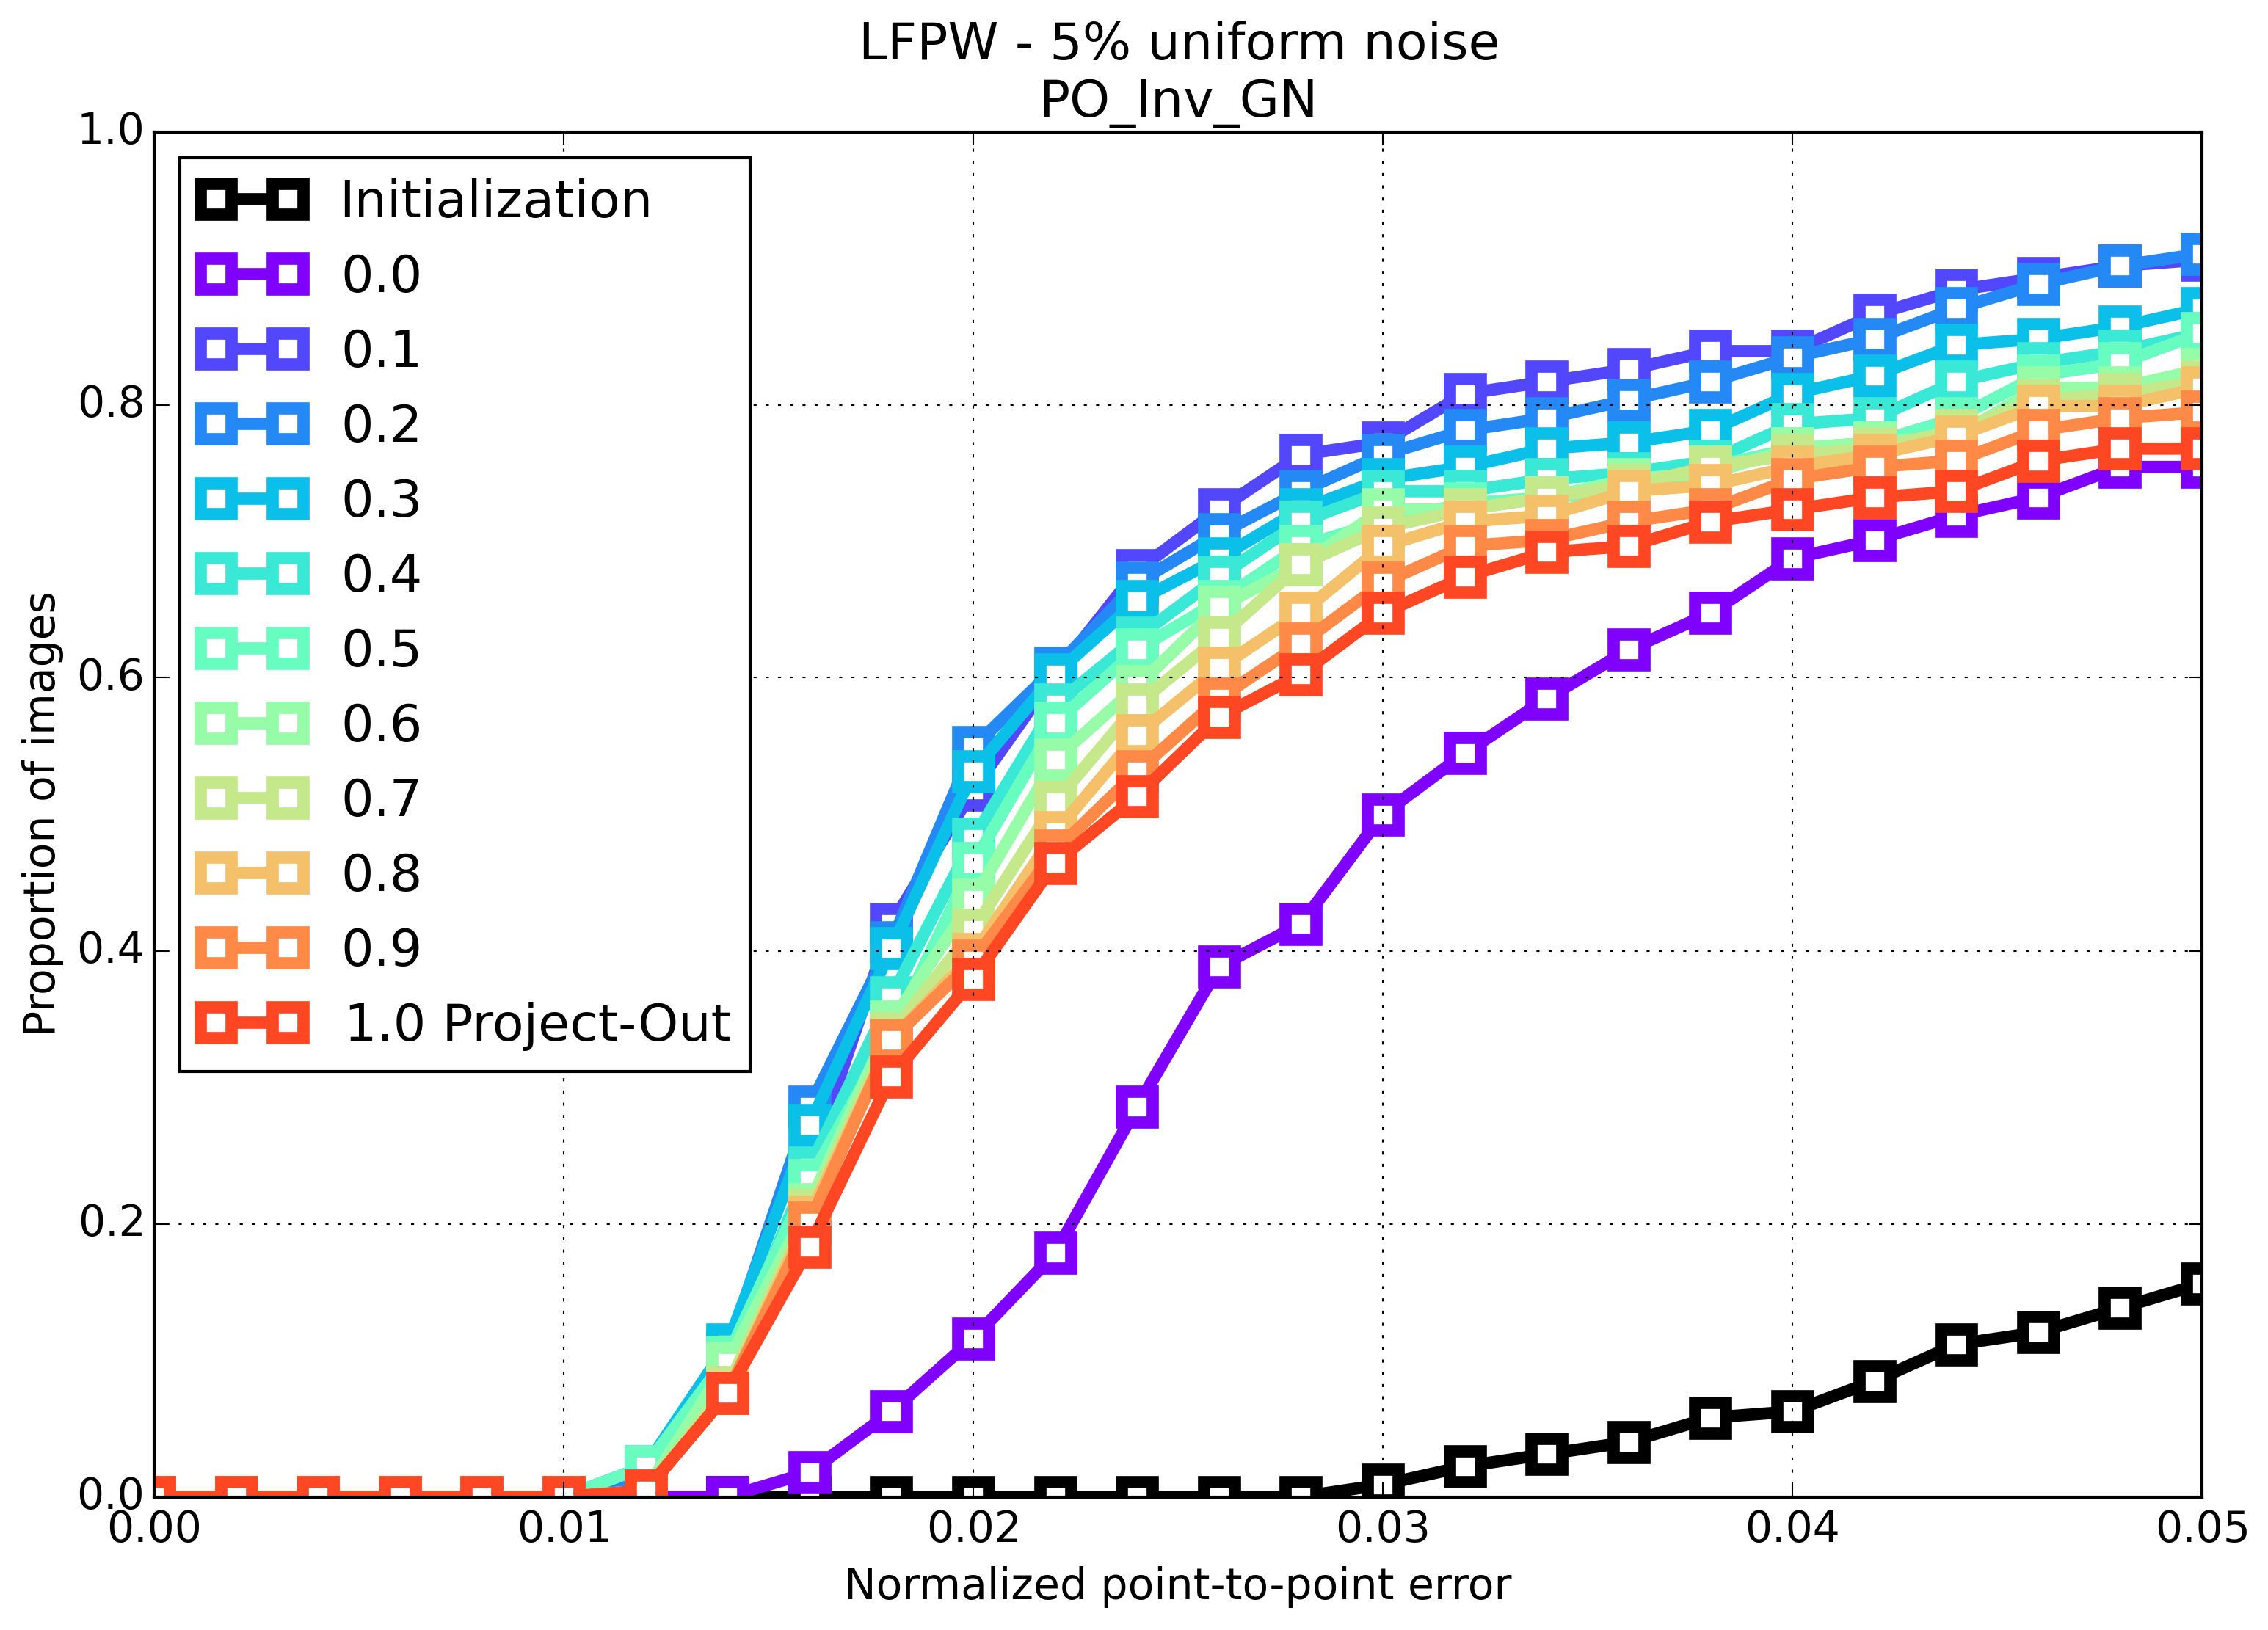
\includegraphics[width=\textwidth]{experiments/rho/ced_po_inv_gn_5.png}
	    \caption{CED on the LFPW test dataset for Project-Out Inverse Gauss-Newton algorithms for different values of $\rho$ and $\gamma$ and initialized with $5\%$ noise.}
	    \label{fig:ced_po_inv_gn}
	\end{subfigure}
	\par\medskip
	\begin{subfigure}{0.48\textwidth}
	    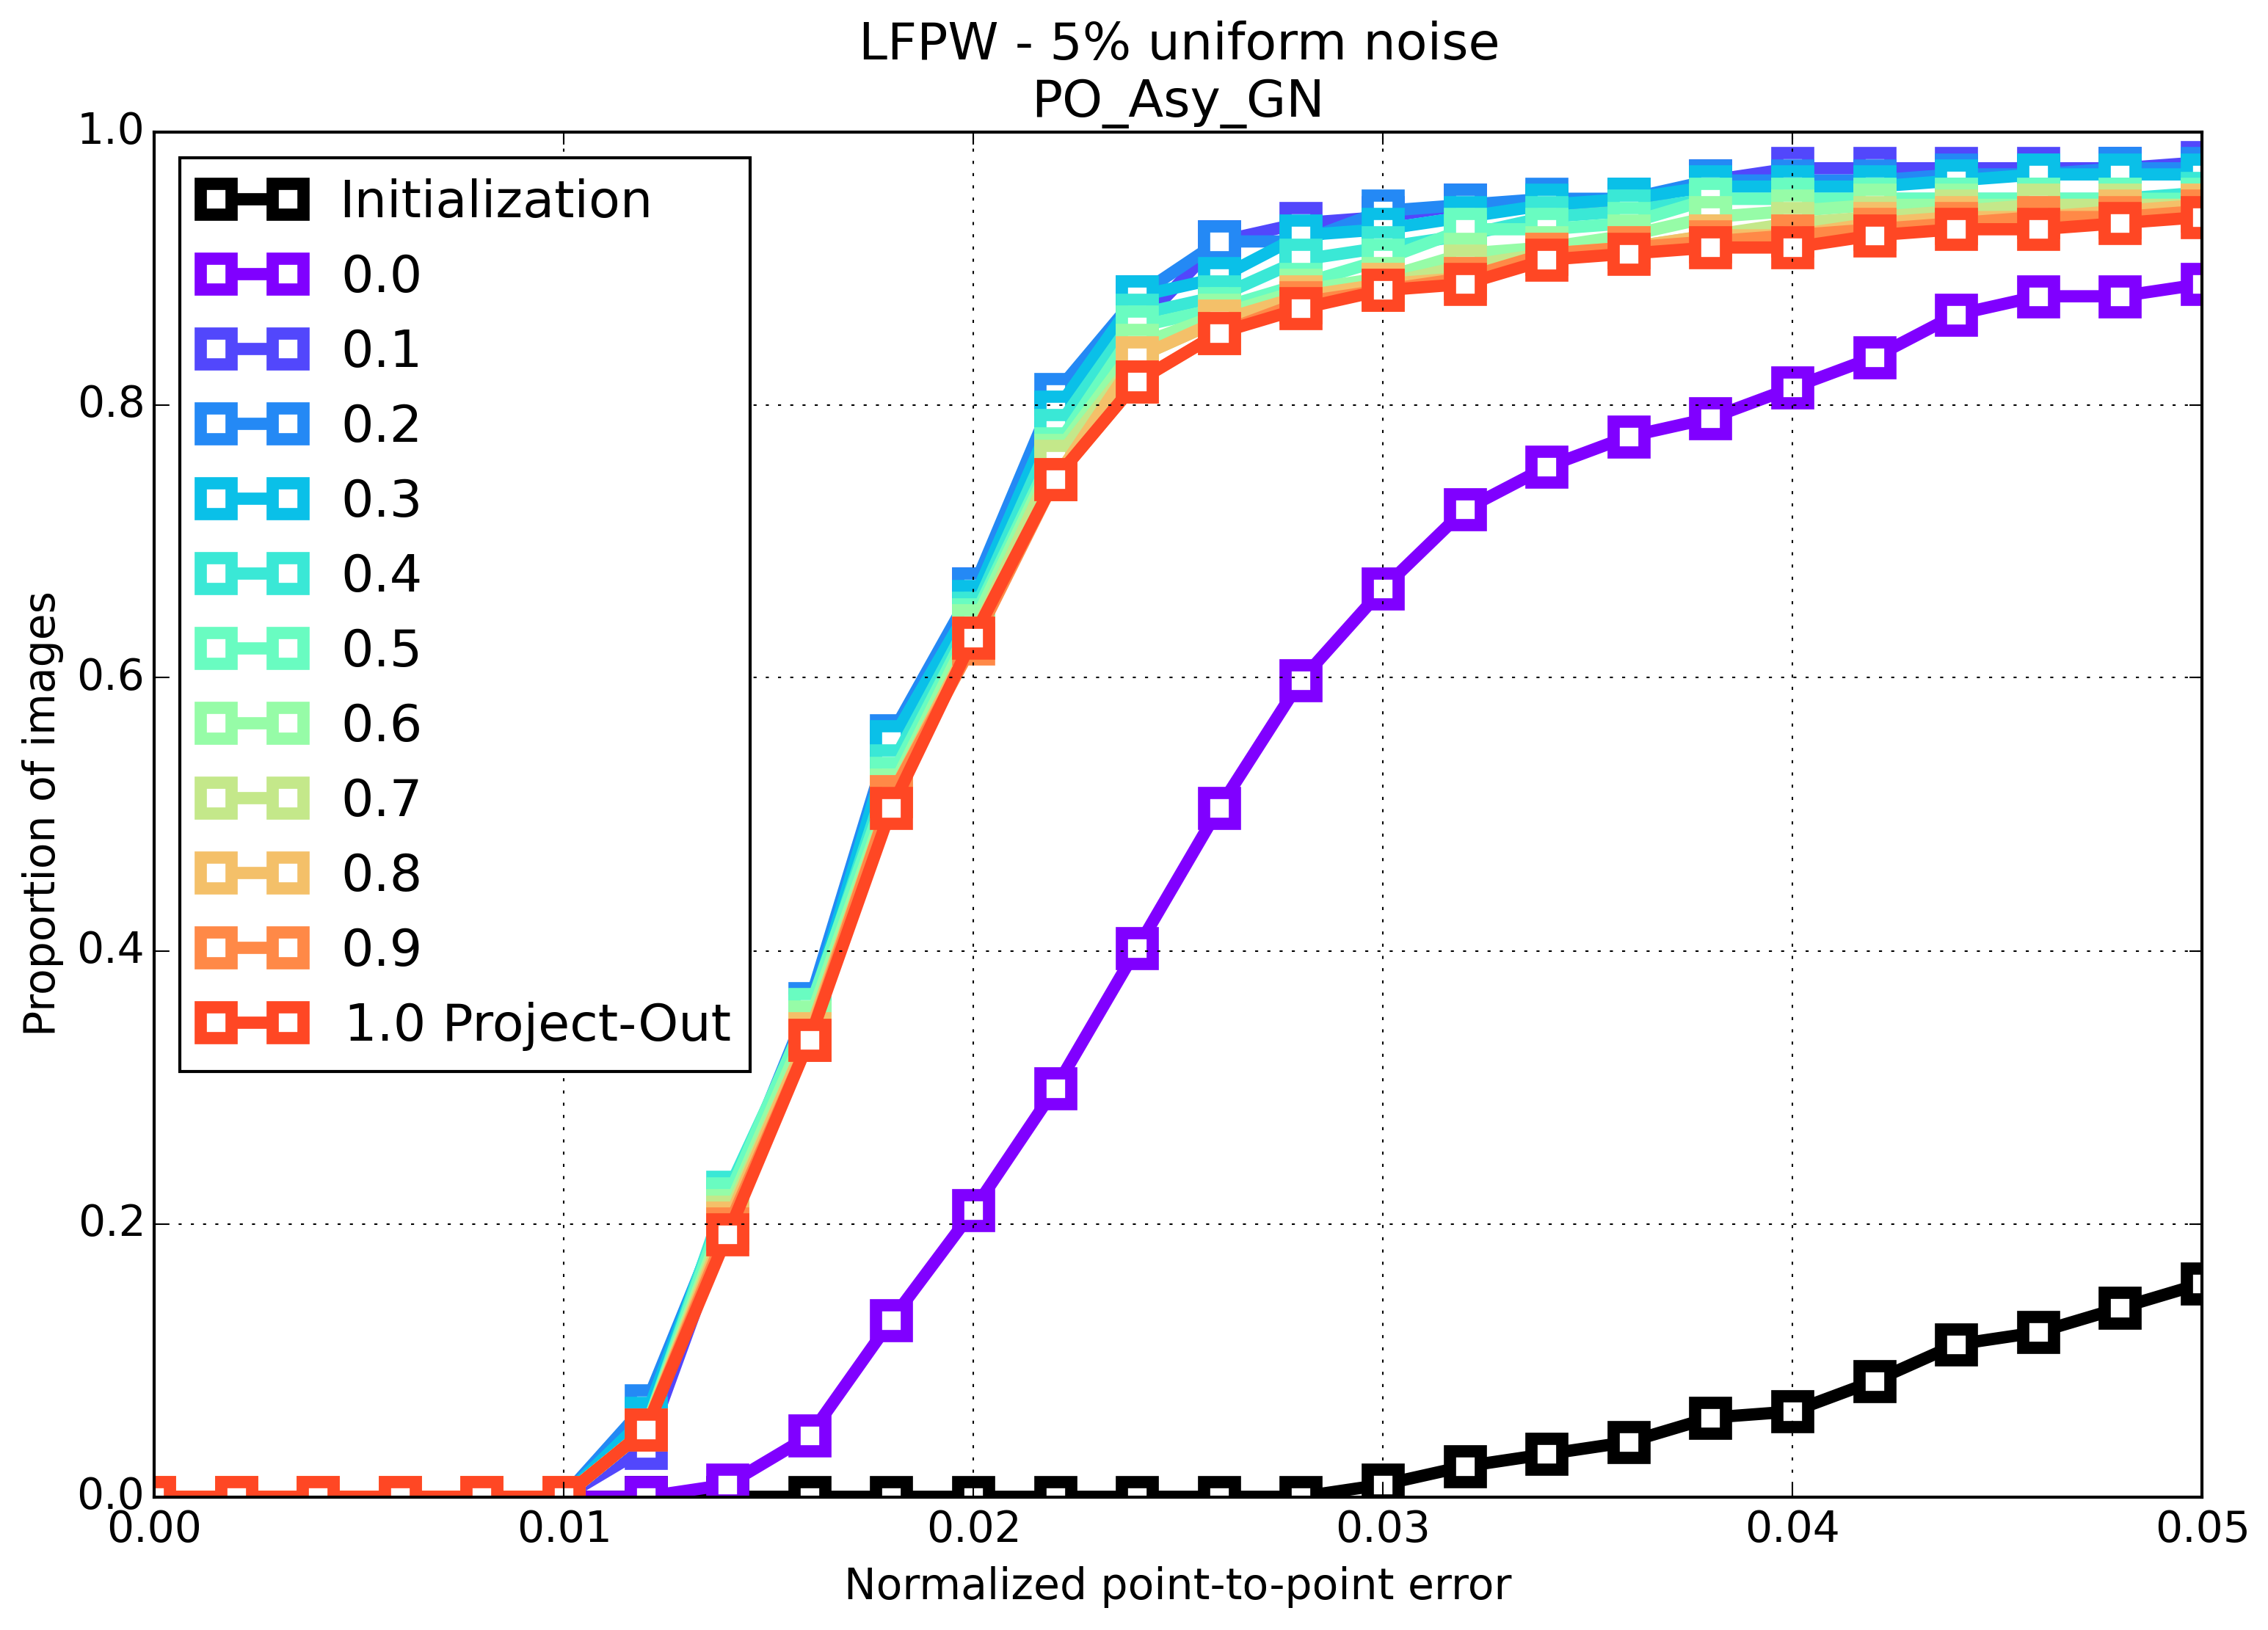
\includegraphics[width=\textwidth]{experiments/rho/ced_po_asy_gn_5.png}
	    \caption{CED on the LFPW test dataset for Project-Out Asymmetric Gauss-Newton algorithms for different values of $\rho$ and $\gamma$ and initialized with $5\%$ noise.}
	    \label{fig:ced_po_asy_gn}
	\end{subfigure}
	\hfill
	\begin{subfigure}{0.48\textwidth}
	    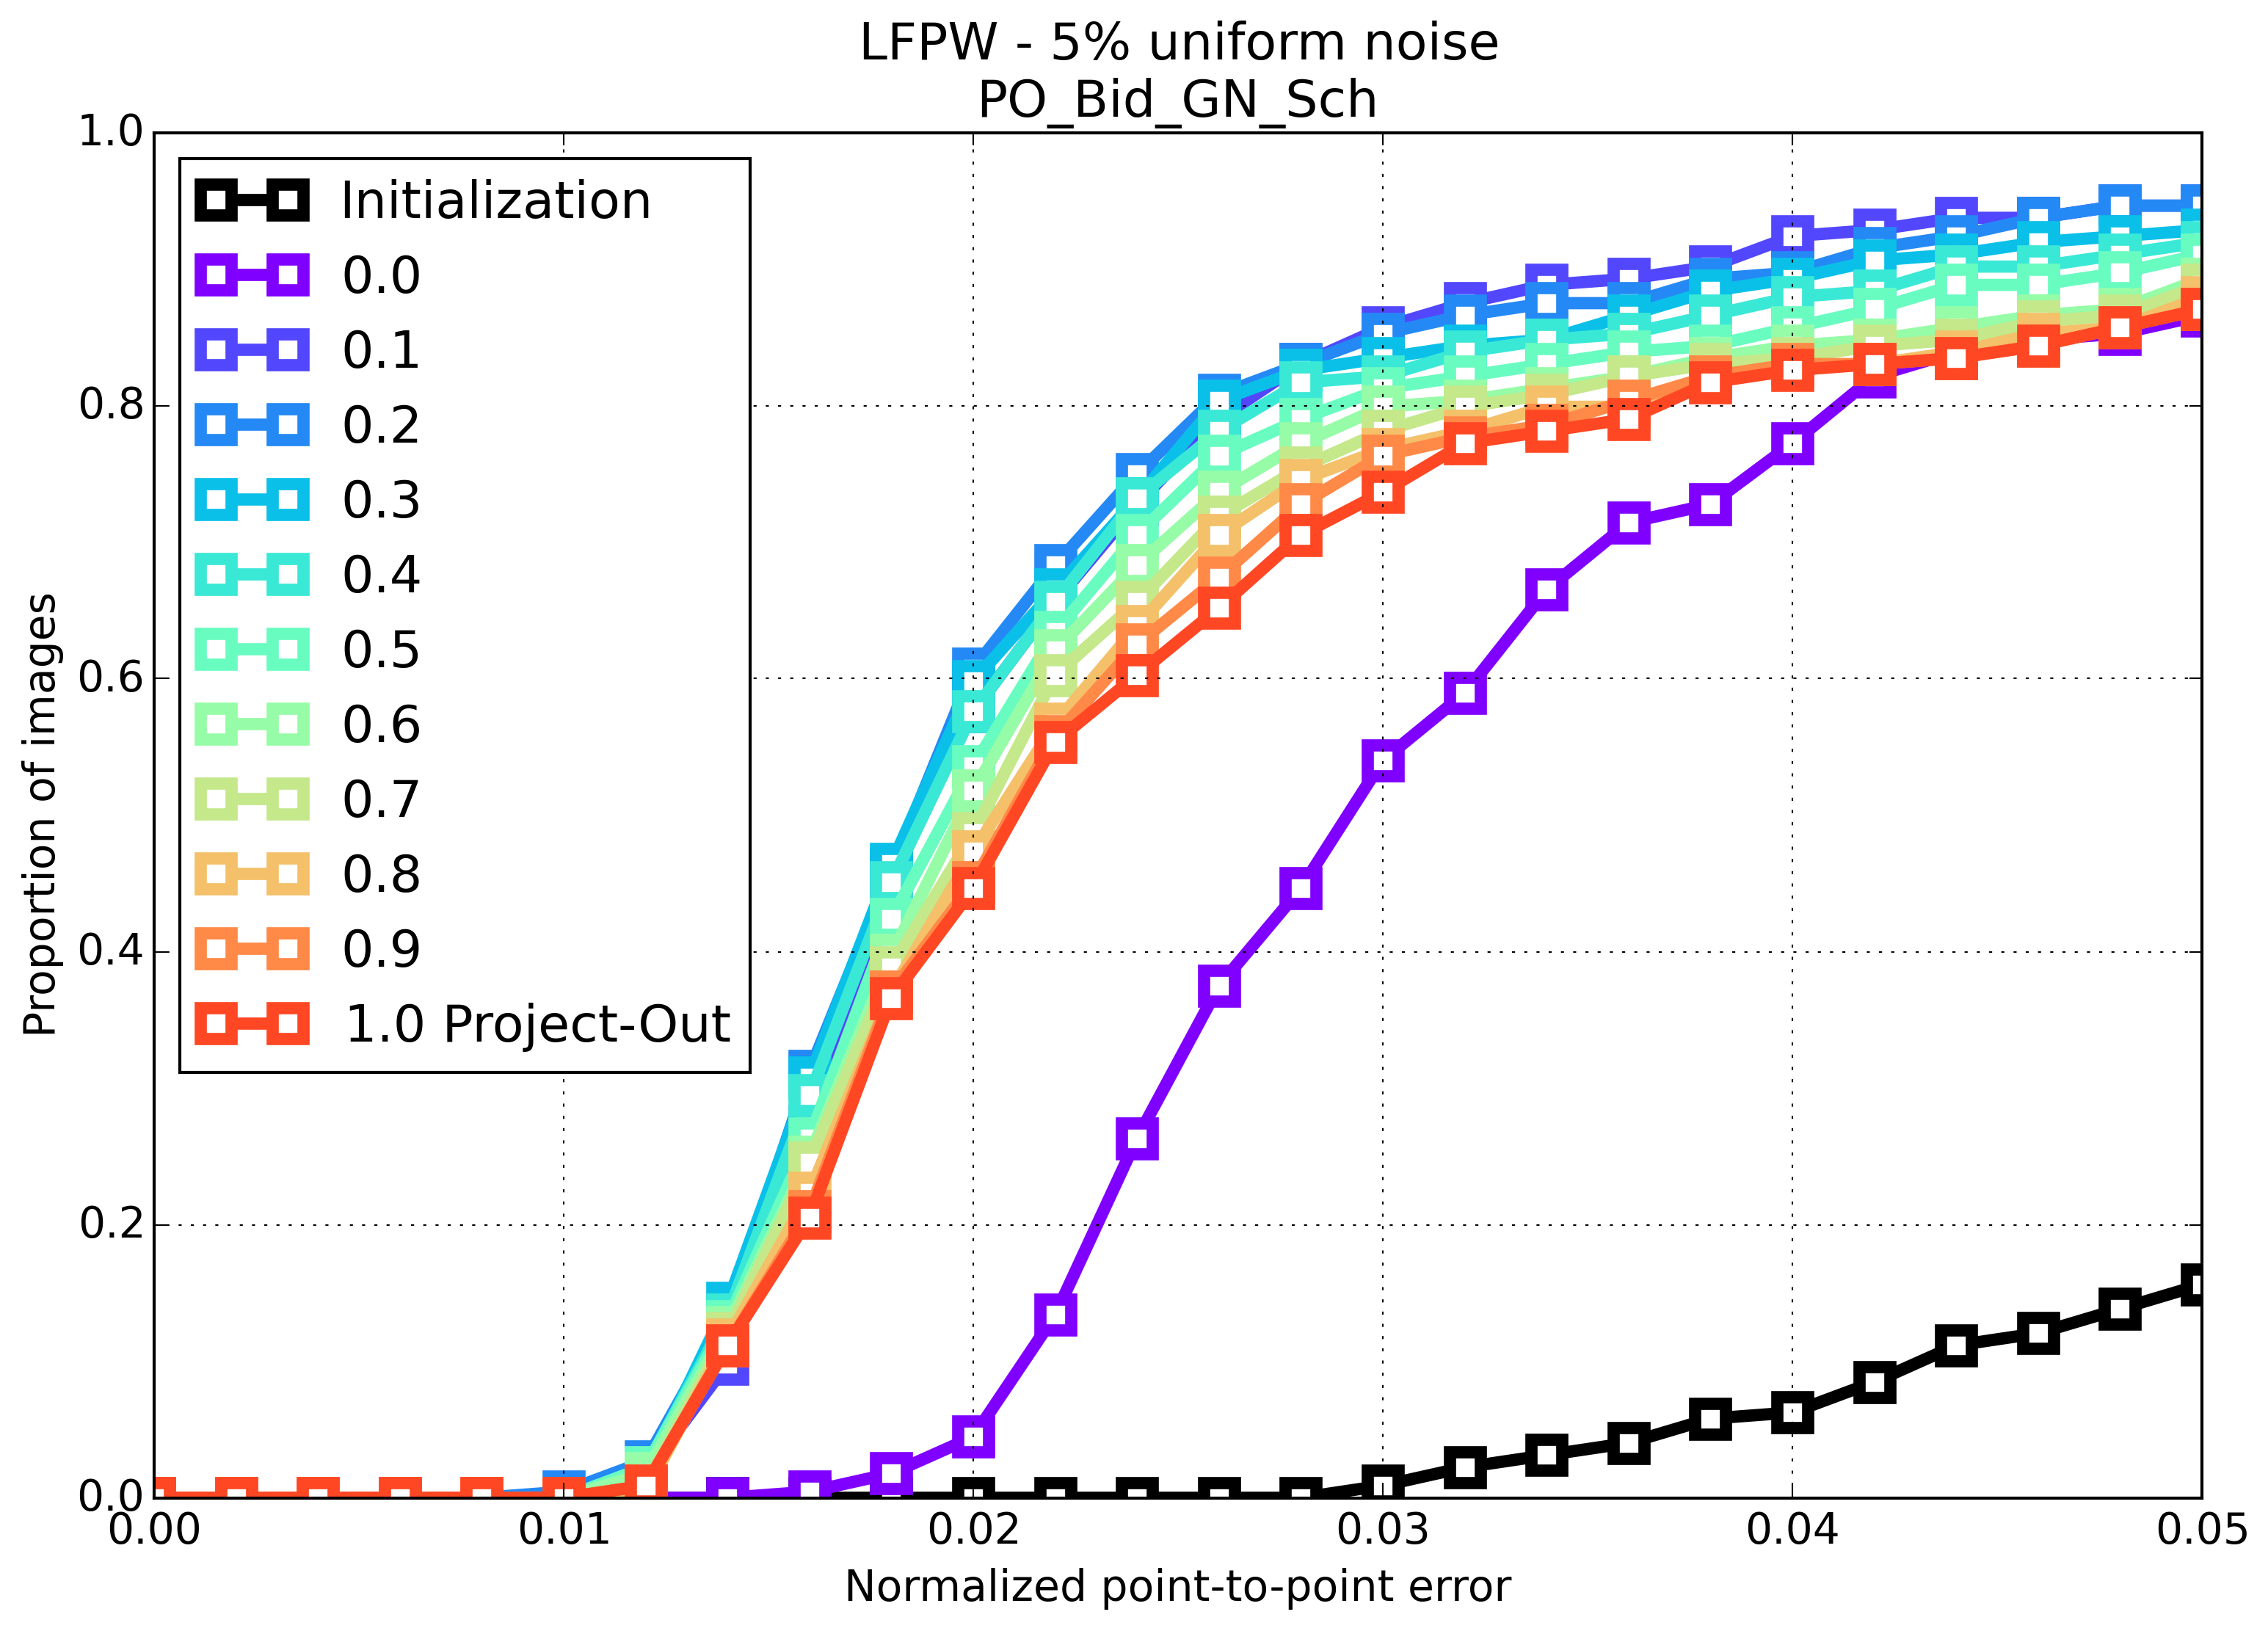
\includegraphics[width=\textwidth]{experiments/rho/ced_po_bid_gn_5.png}
	    \caption{CED on the LFPW test dataset for Project-Out Bidirectional Gauss-Newton algorithms for different values of $\rho$ and $\gamma$ and initialized with $5\%$ noise.}
	    \label{fig:ced_po_bid_gn}
	\end{subfigure}
	\caption{Results quantifying the effect of varying the value of the parameters $\rho$ and $\gamma$ in Project-Out Gauss-Newton algorithms.}
	\label{fig:rho}
\end{figure*}

% \begin{figure}[h!]
% 	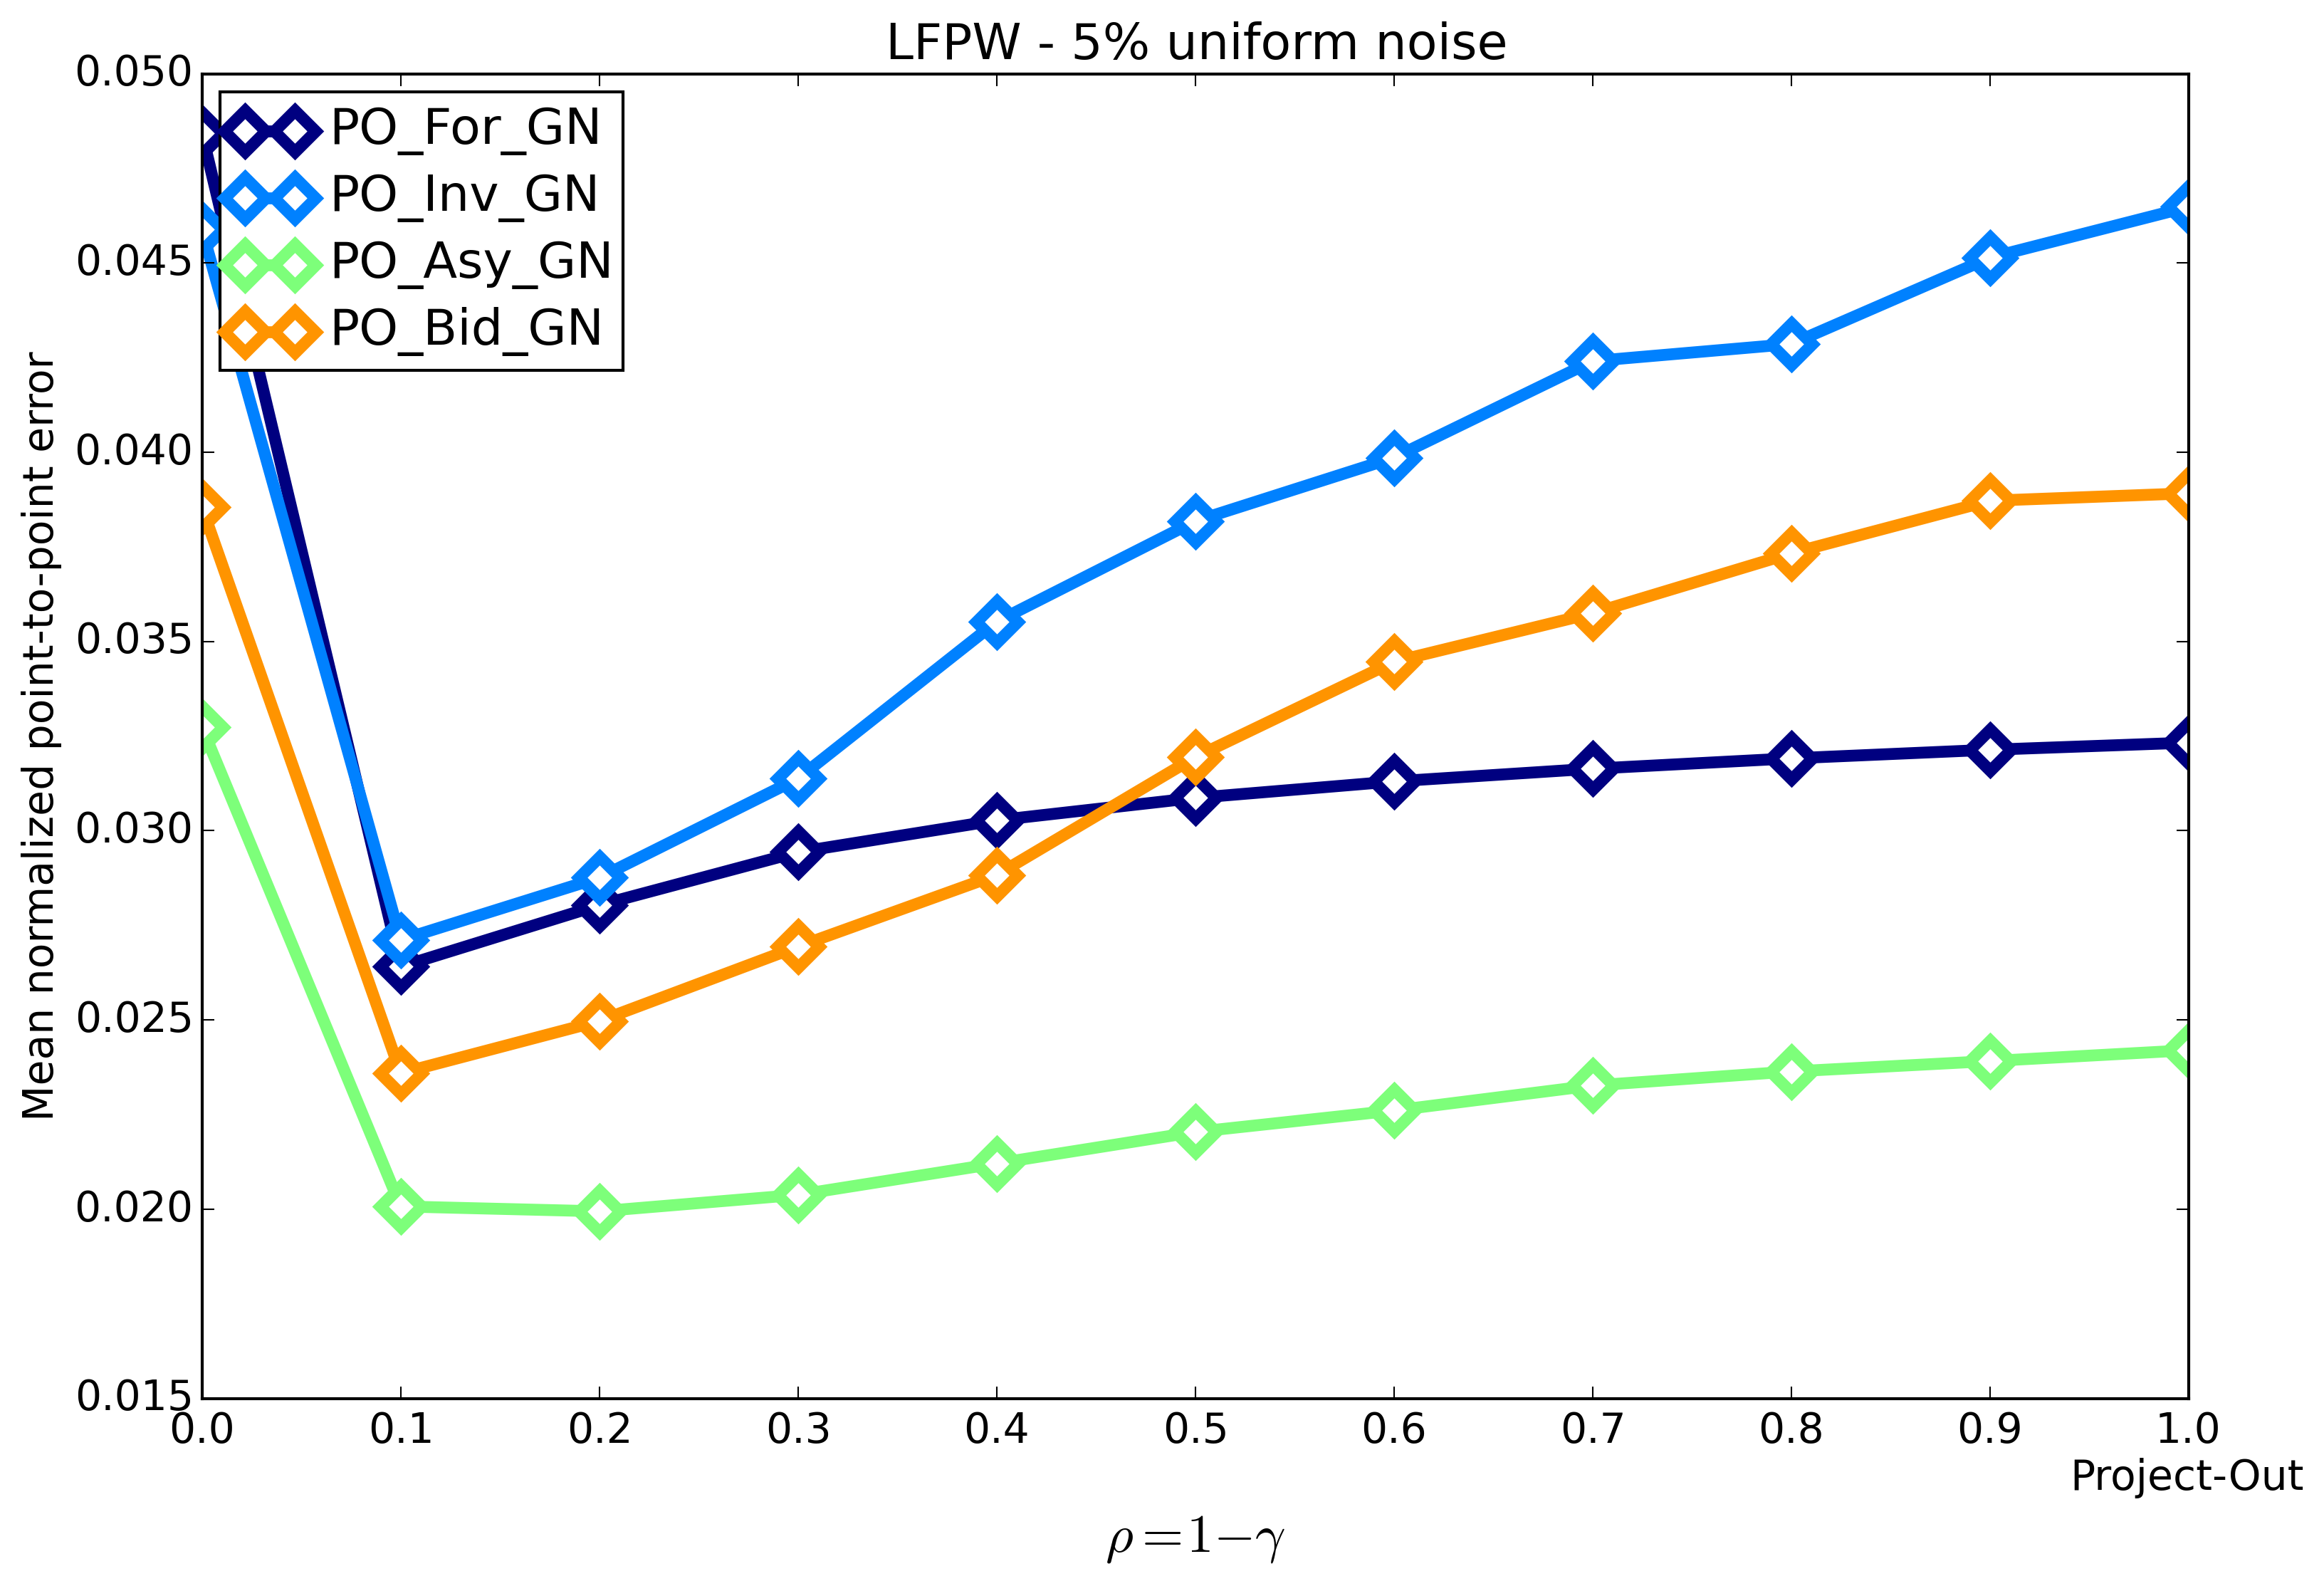
\includegraphics[width=0.48\textwidth]{experiments/rho/mean_error_vs_rho_5.png}
%     \caption{Mean normalized point-to-point error vs rho on the LFPW test dataset for all PO Gauss-Newton algorithms initialized with $5\%$ uniform noise.}
%     \label{fig:rho_5}
% \end{figure}


\subsubsection{Optimal asymmetric composition}

This experiment quantifies the effect that varying the value of the parameters $\alpha \in [0, 1]$ and $\beta = 1 -\alpha$ in Equation \ref{eq:ssd_ac} has in the fitting accuracy obtained by the asymmetric algorithms. Note that for $\alpha=1$, $\beta=0$ and $\alpha=0$, $\beta=1$ these algorithms reduce to their forward and inverse versions respectively. Remember that, in previous experiments, we used the symmetric case $\alpha=\beta=0.5$ to generate the results reported for asymmetric algorithms.

We again repeat the experimental set up described in the first experiments and report the fitting accuracy obtained by the Project Out and SSD Asymmetric Gauss-Newton algorithms for different values of the parameters $\alpha$ and $\beta$. Results are shown in Figure \ref{fig:alpha}. 

\begin{figure*}[h!]
	\centering
	\begin{subfigure}{\textwidth}
	    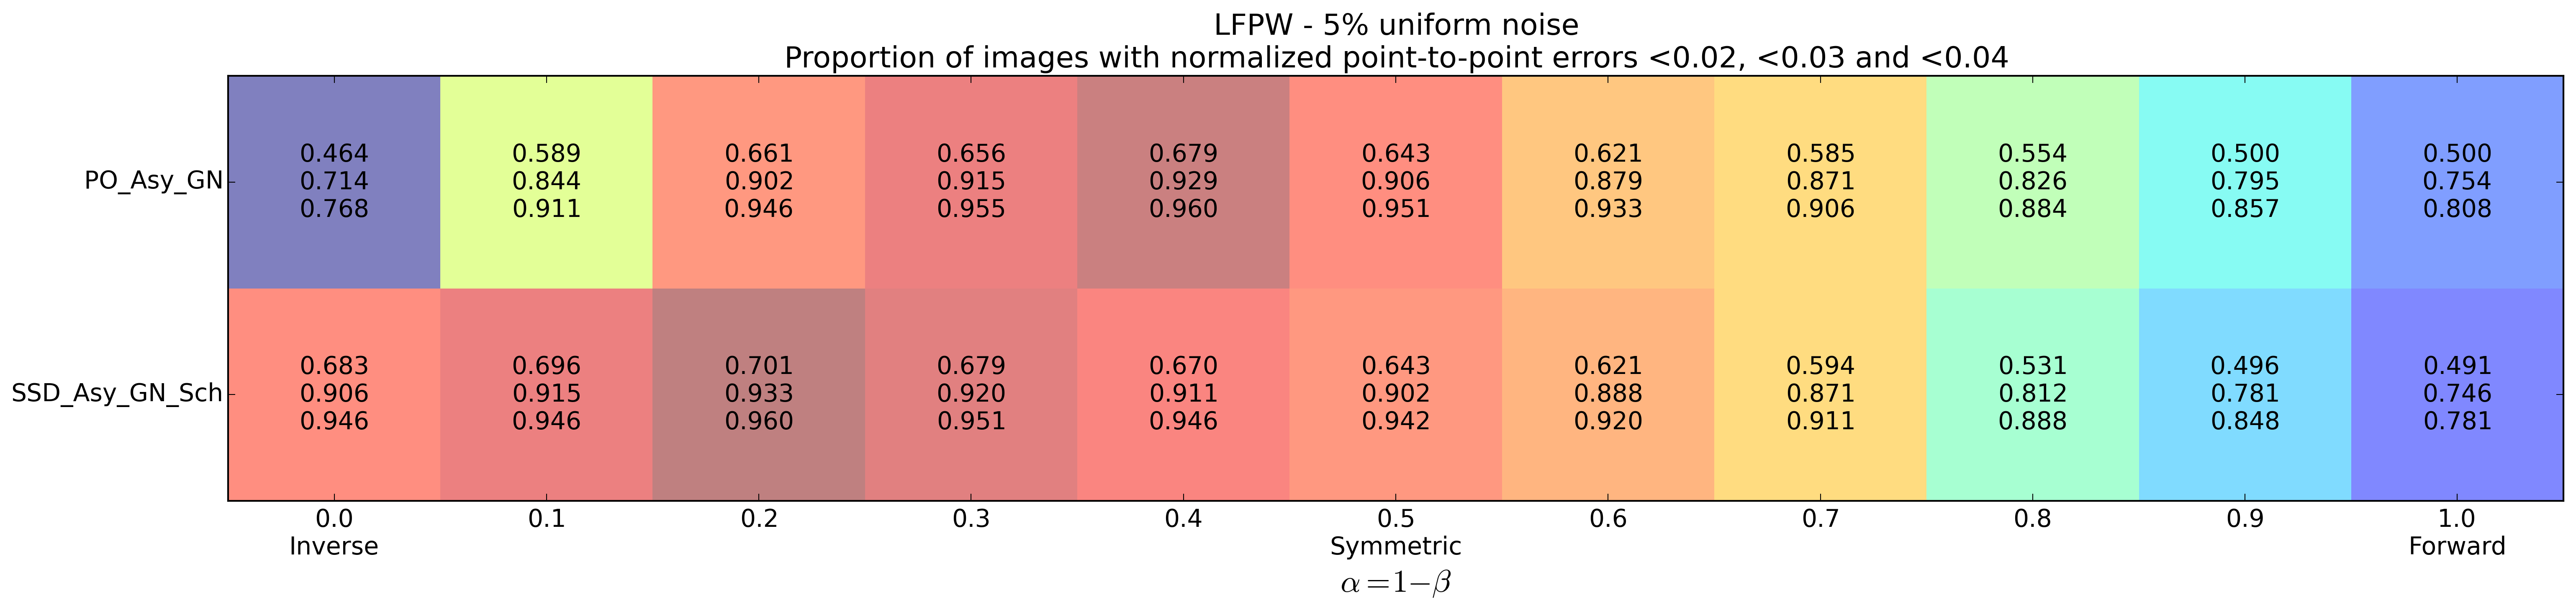
\includegraphics[width=\textwidth]{experiments/alpha/asy_gn_vs_alpha_5.png}
	    \caption{Proportion of images with normalized point-to-point errors smaller than $0.02$, $0.03$ and $0.04$ for the Project-Out and SSD Asymmetric Gauss-Newton algorithms values of $\alpha$ and $\beta$ and initialized with $5\%$ noise.}
	    \label{fig:ced_po_asy_gn}
	\end{subfigure}
	\par\medskip
	\begin{subfigure}{0.48\textwidth}
	    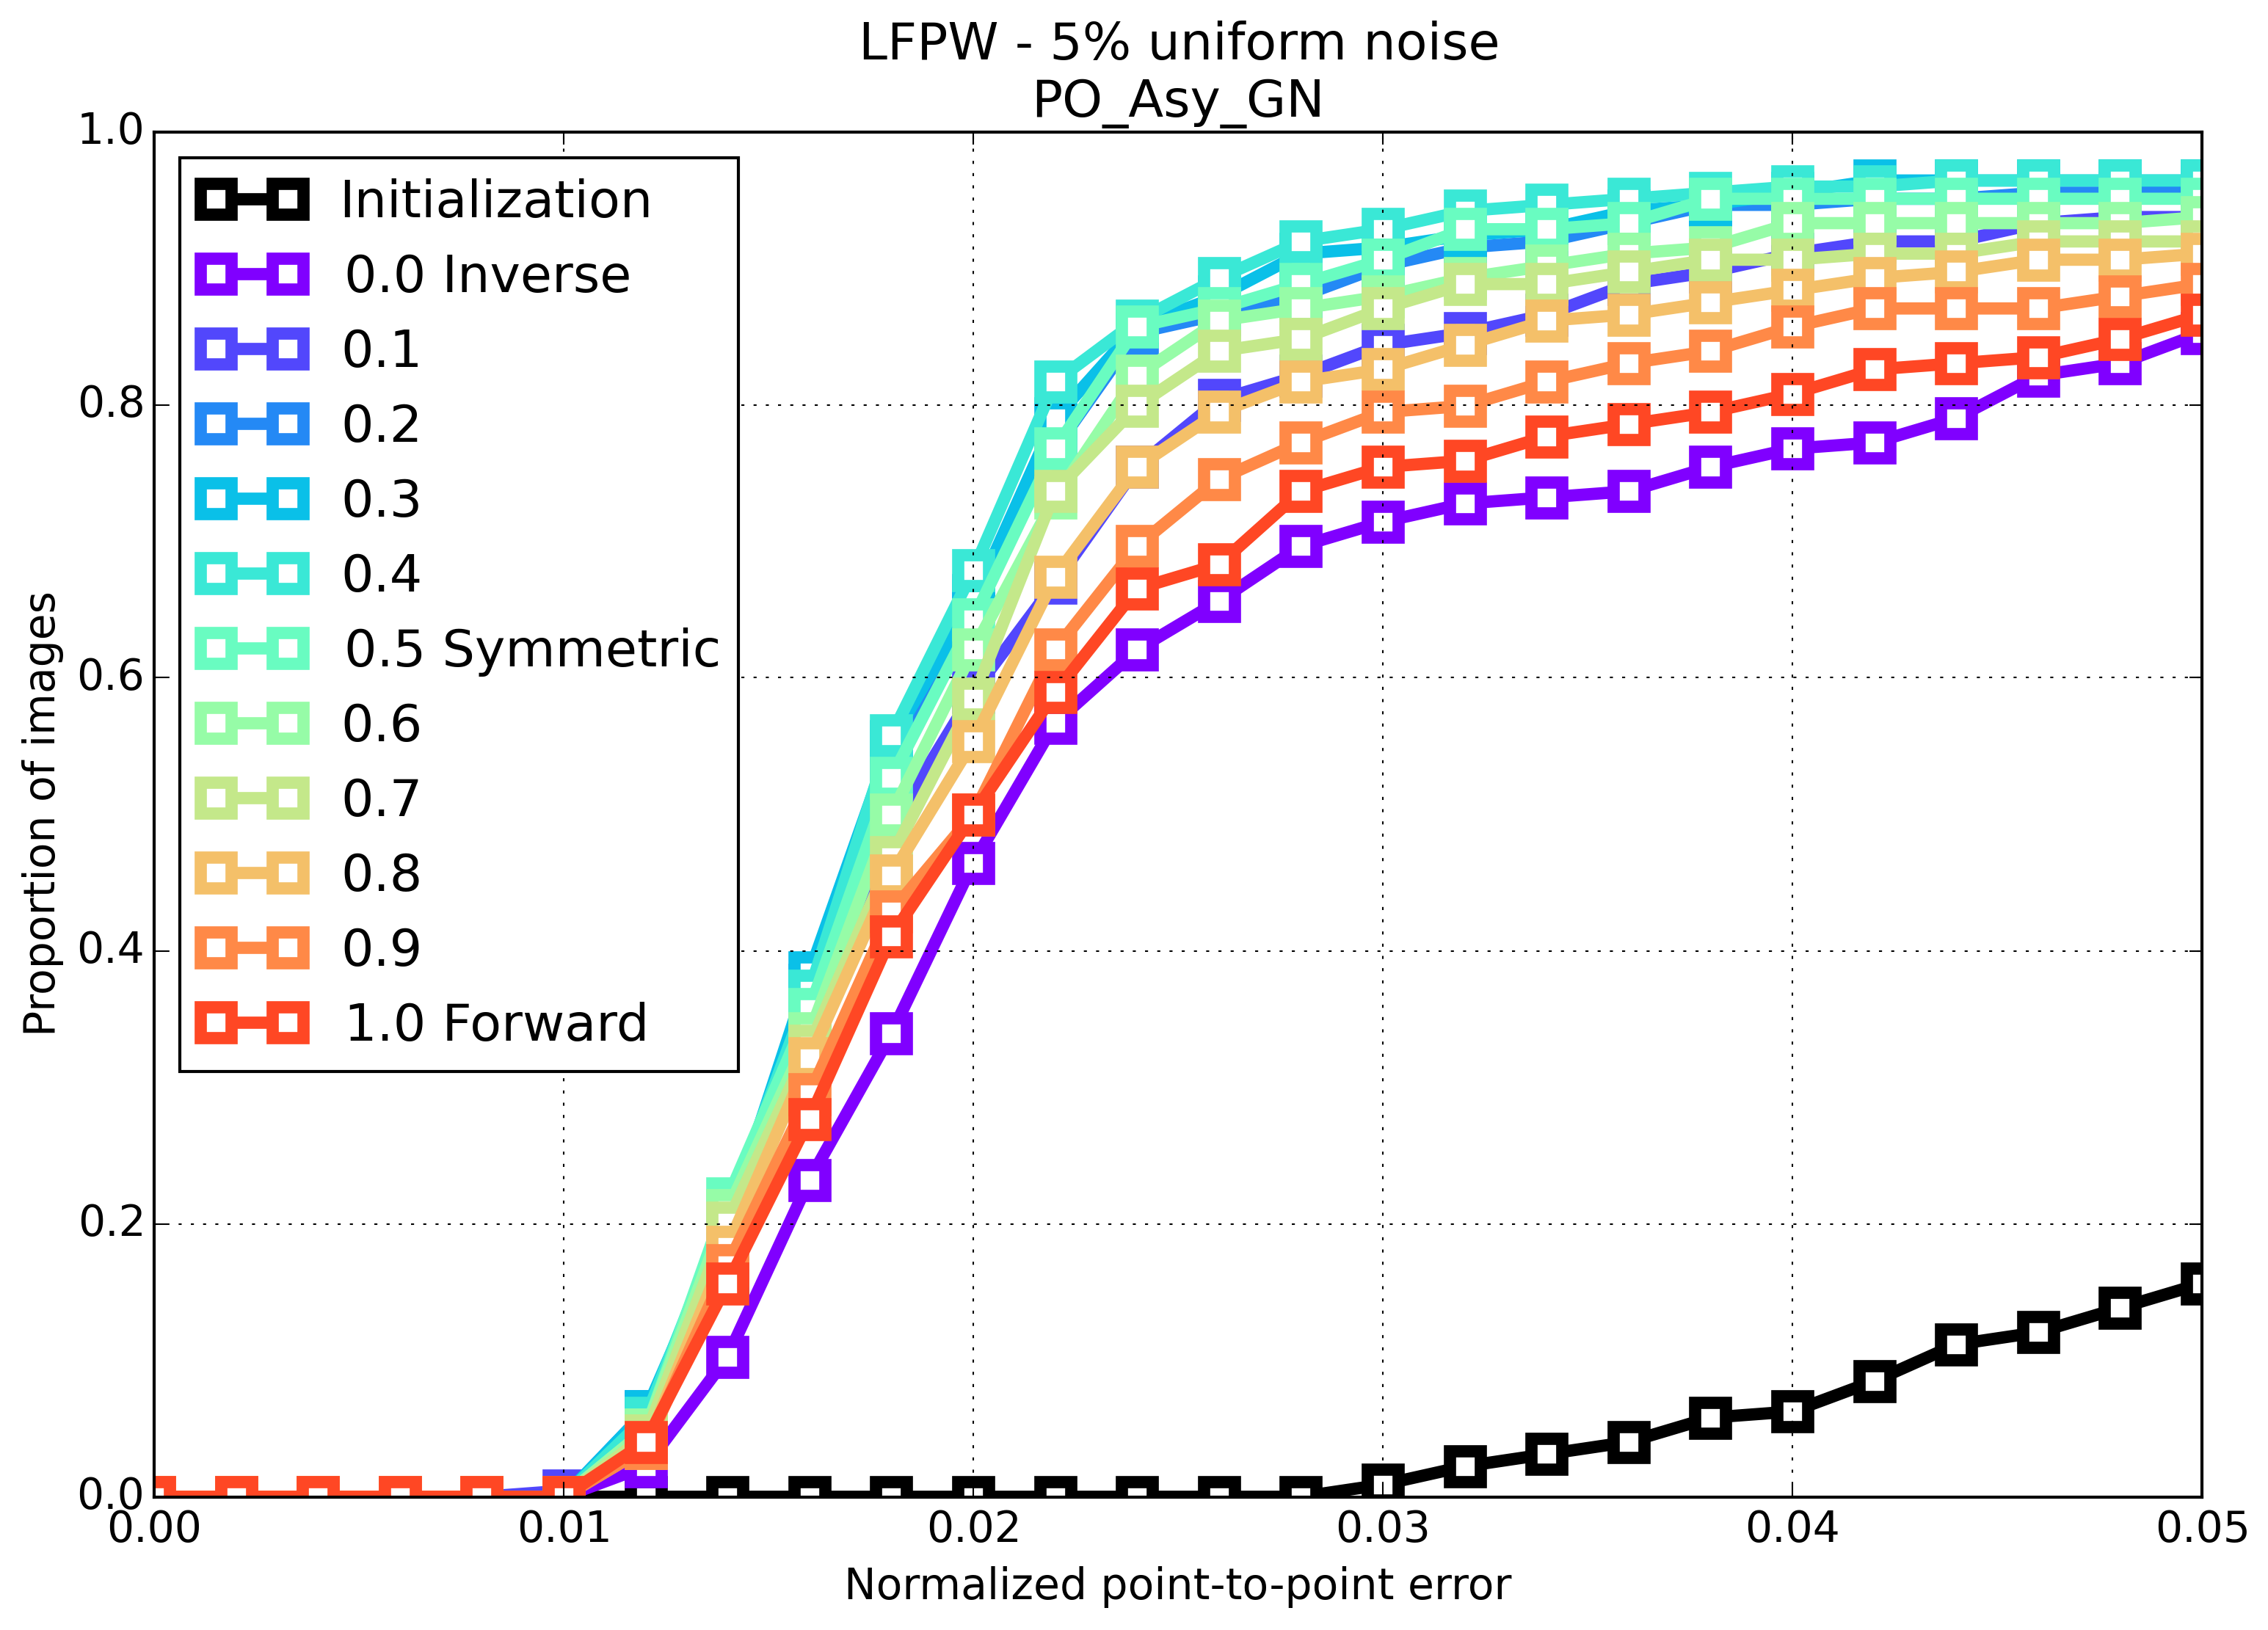
\includegraphics[width=\textwidth]{experiments/alpha/ced_po_asy_gn_5.png}
	    \caption{CED on the LFPW test dataset for Project-Out Asymmetric Gauss-Newton algorithm for different values of $\alpha$ and $\beta$ and initialized with $5\%$ noise.}
	    \label{fig:ced_po_for_gn}
	\end{subfigure}
	\hfill
	\begin{subfigure}{0.48\textwidth}
	    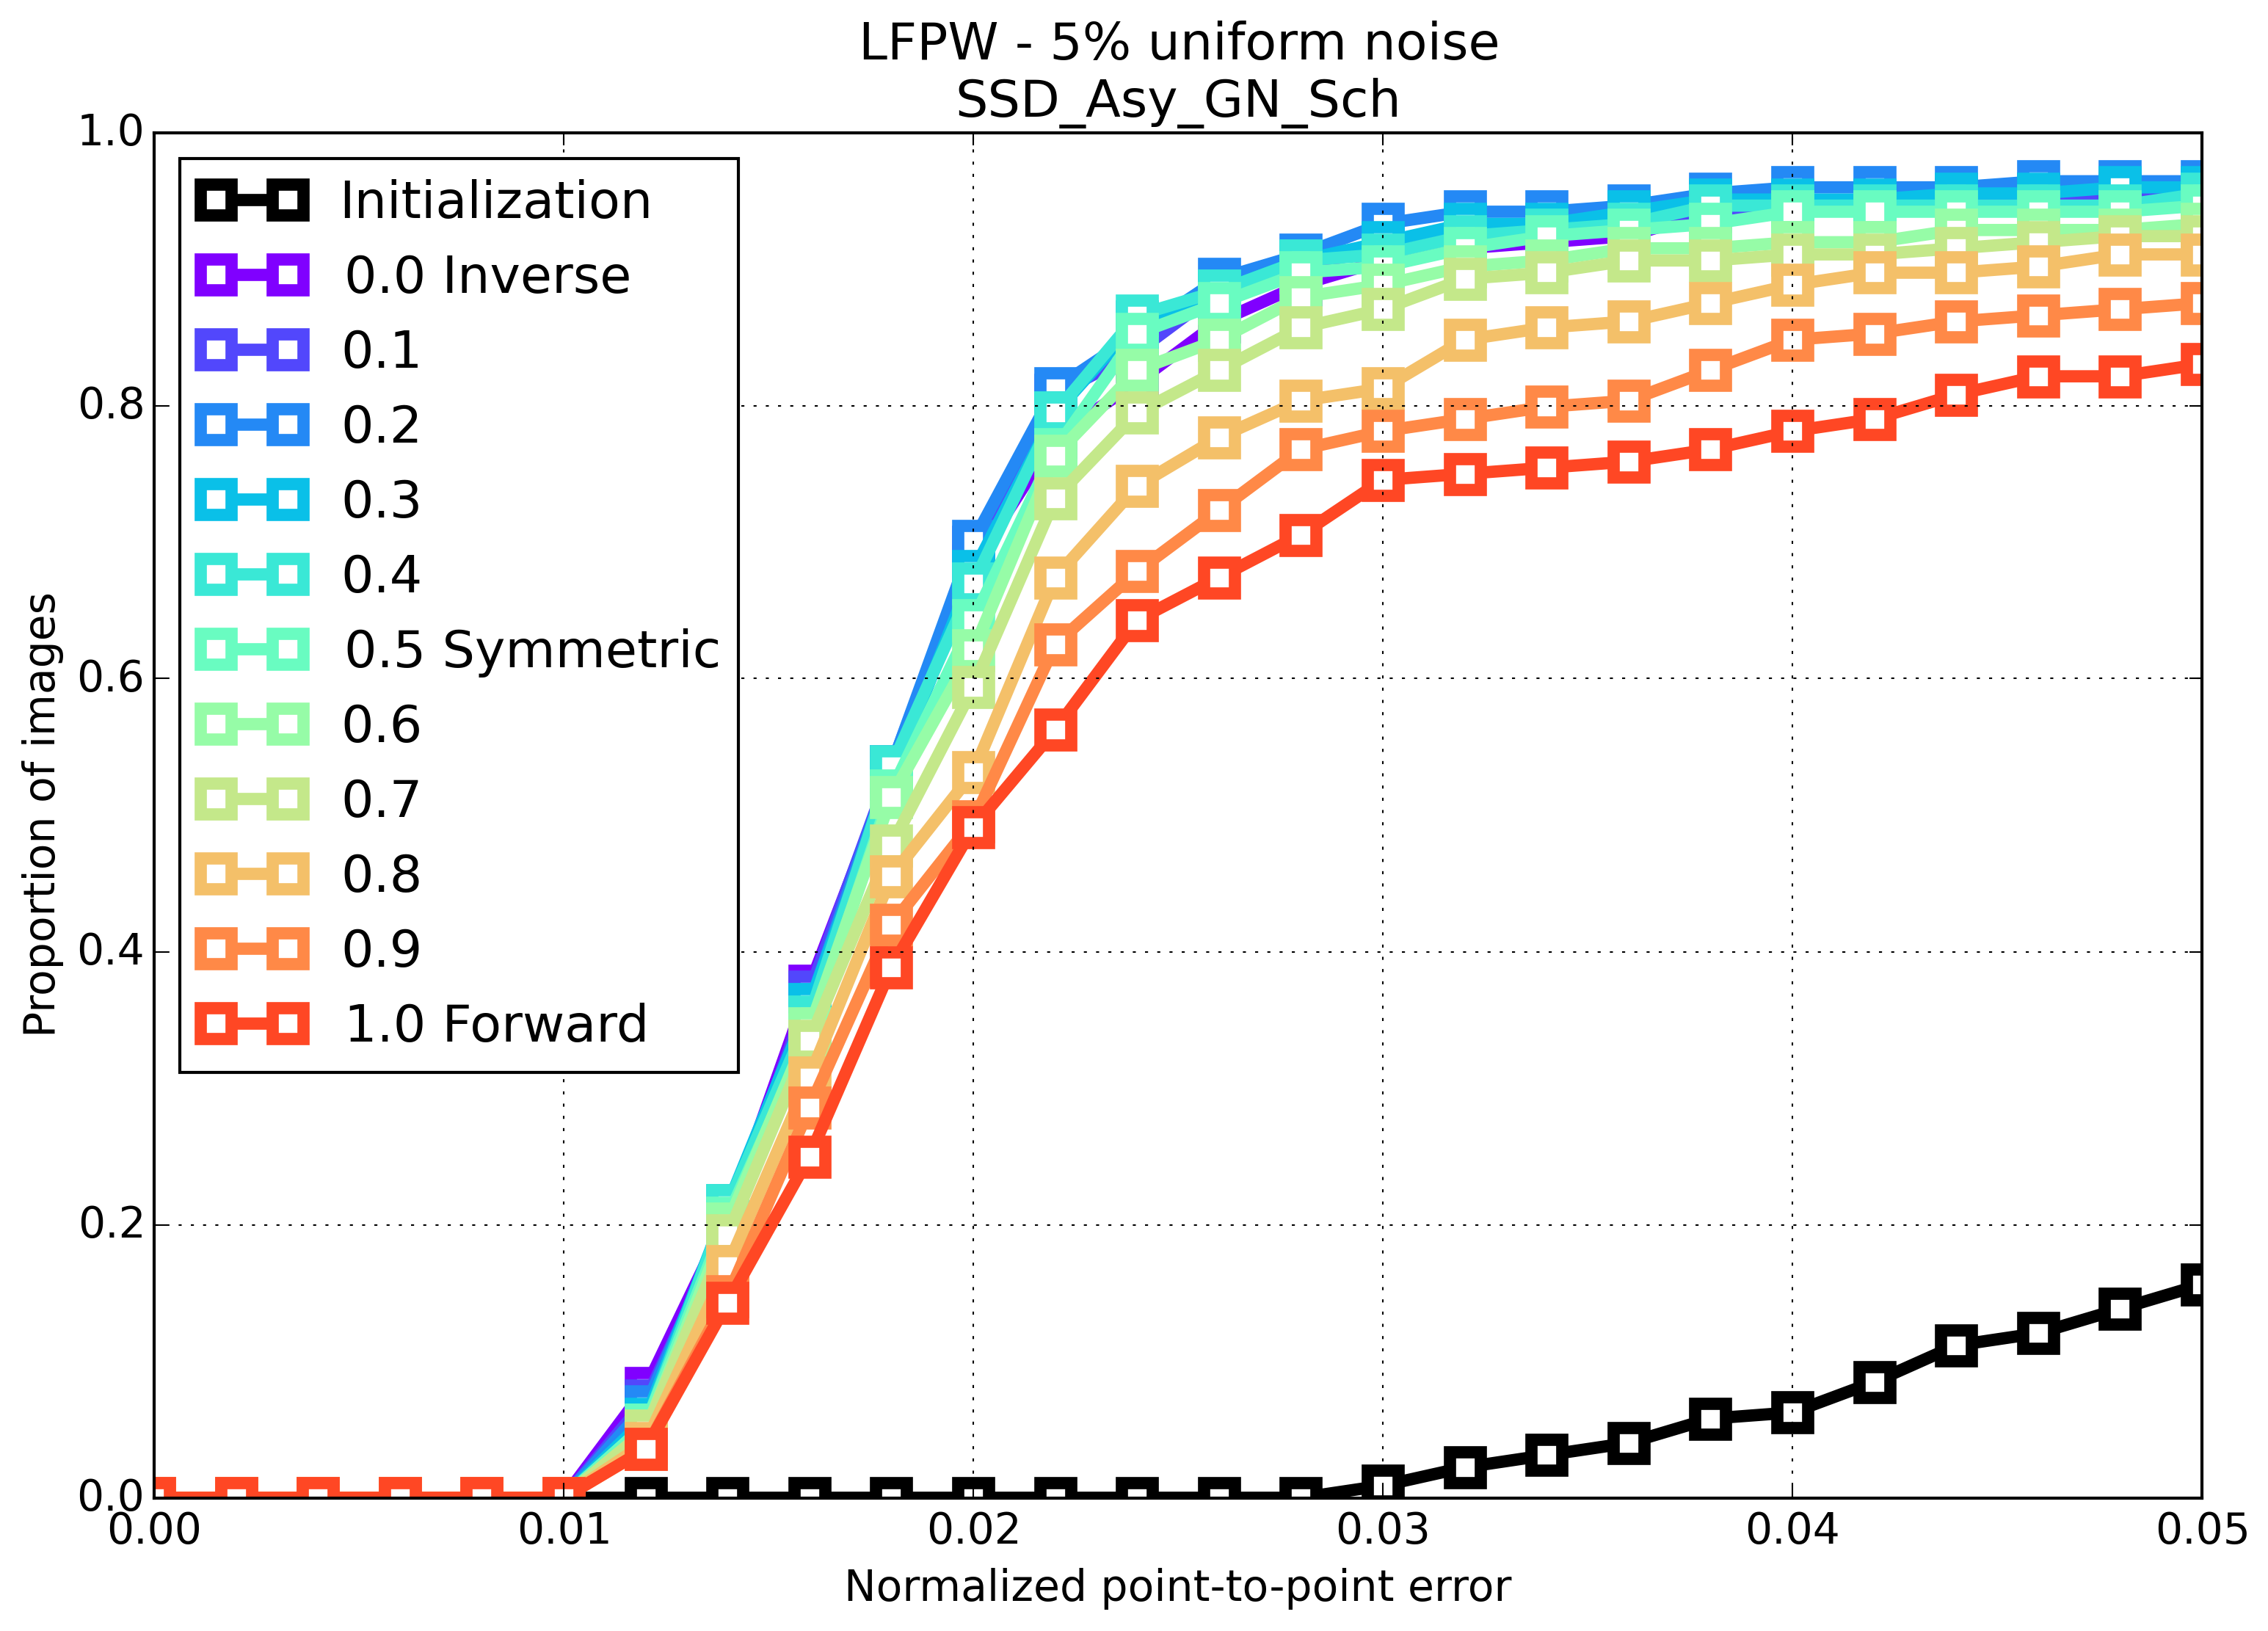
\includegraphics[width=\textwidth]{experiments/alpha/ced_ssd_asy_gn_5.png}
	    \caption{CED on the LFPW test dataset for the the SSD Asymmetric Gauss-Newton algorithm for different values of $\alpha$ and $\beta$ and initialized with $5\%$ noise.}
	    \label{fig:ced_po_inv_gn}
	\end{subfigure}
	\label{fig:alpha}
	\caption{Results quantifying the effect of varying the value of the parameters $\alpha$ and $\beta$ in Asymmetric algorithms.}
\end{figure*}

% \begin{figure}[h!]
%     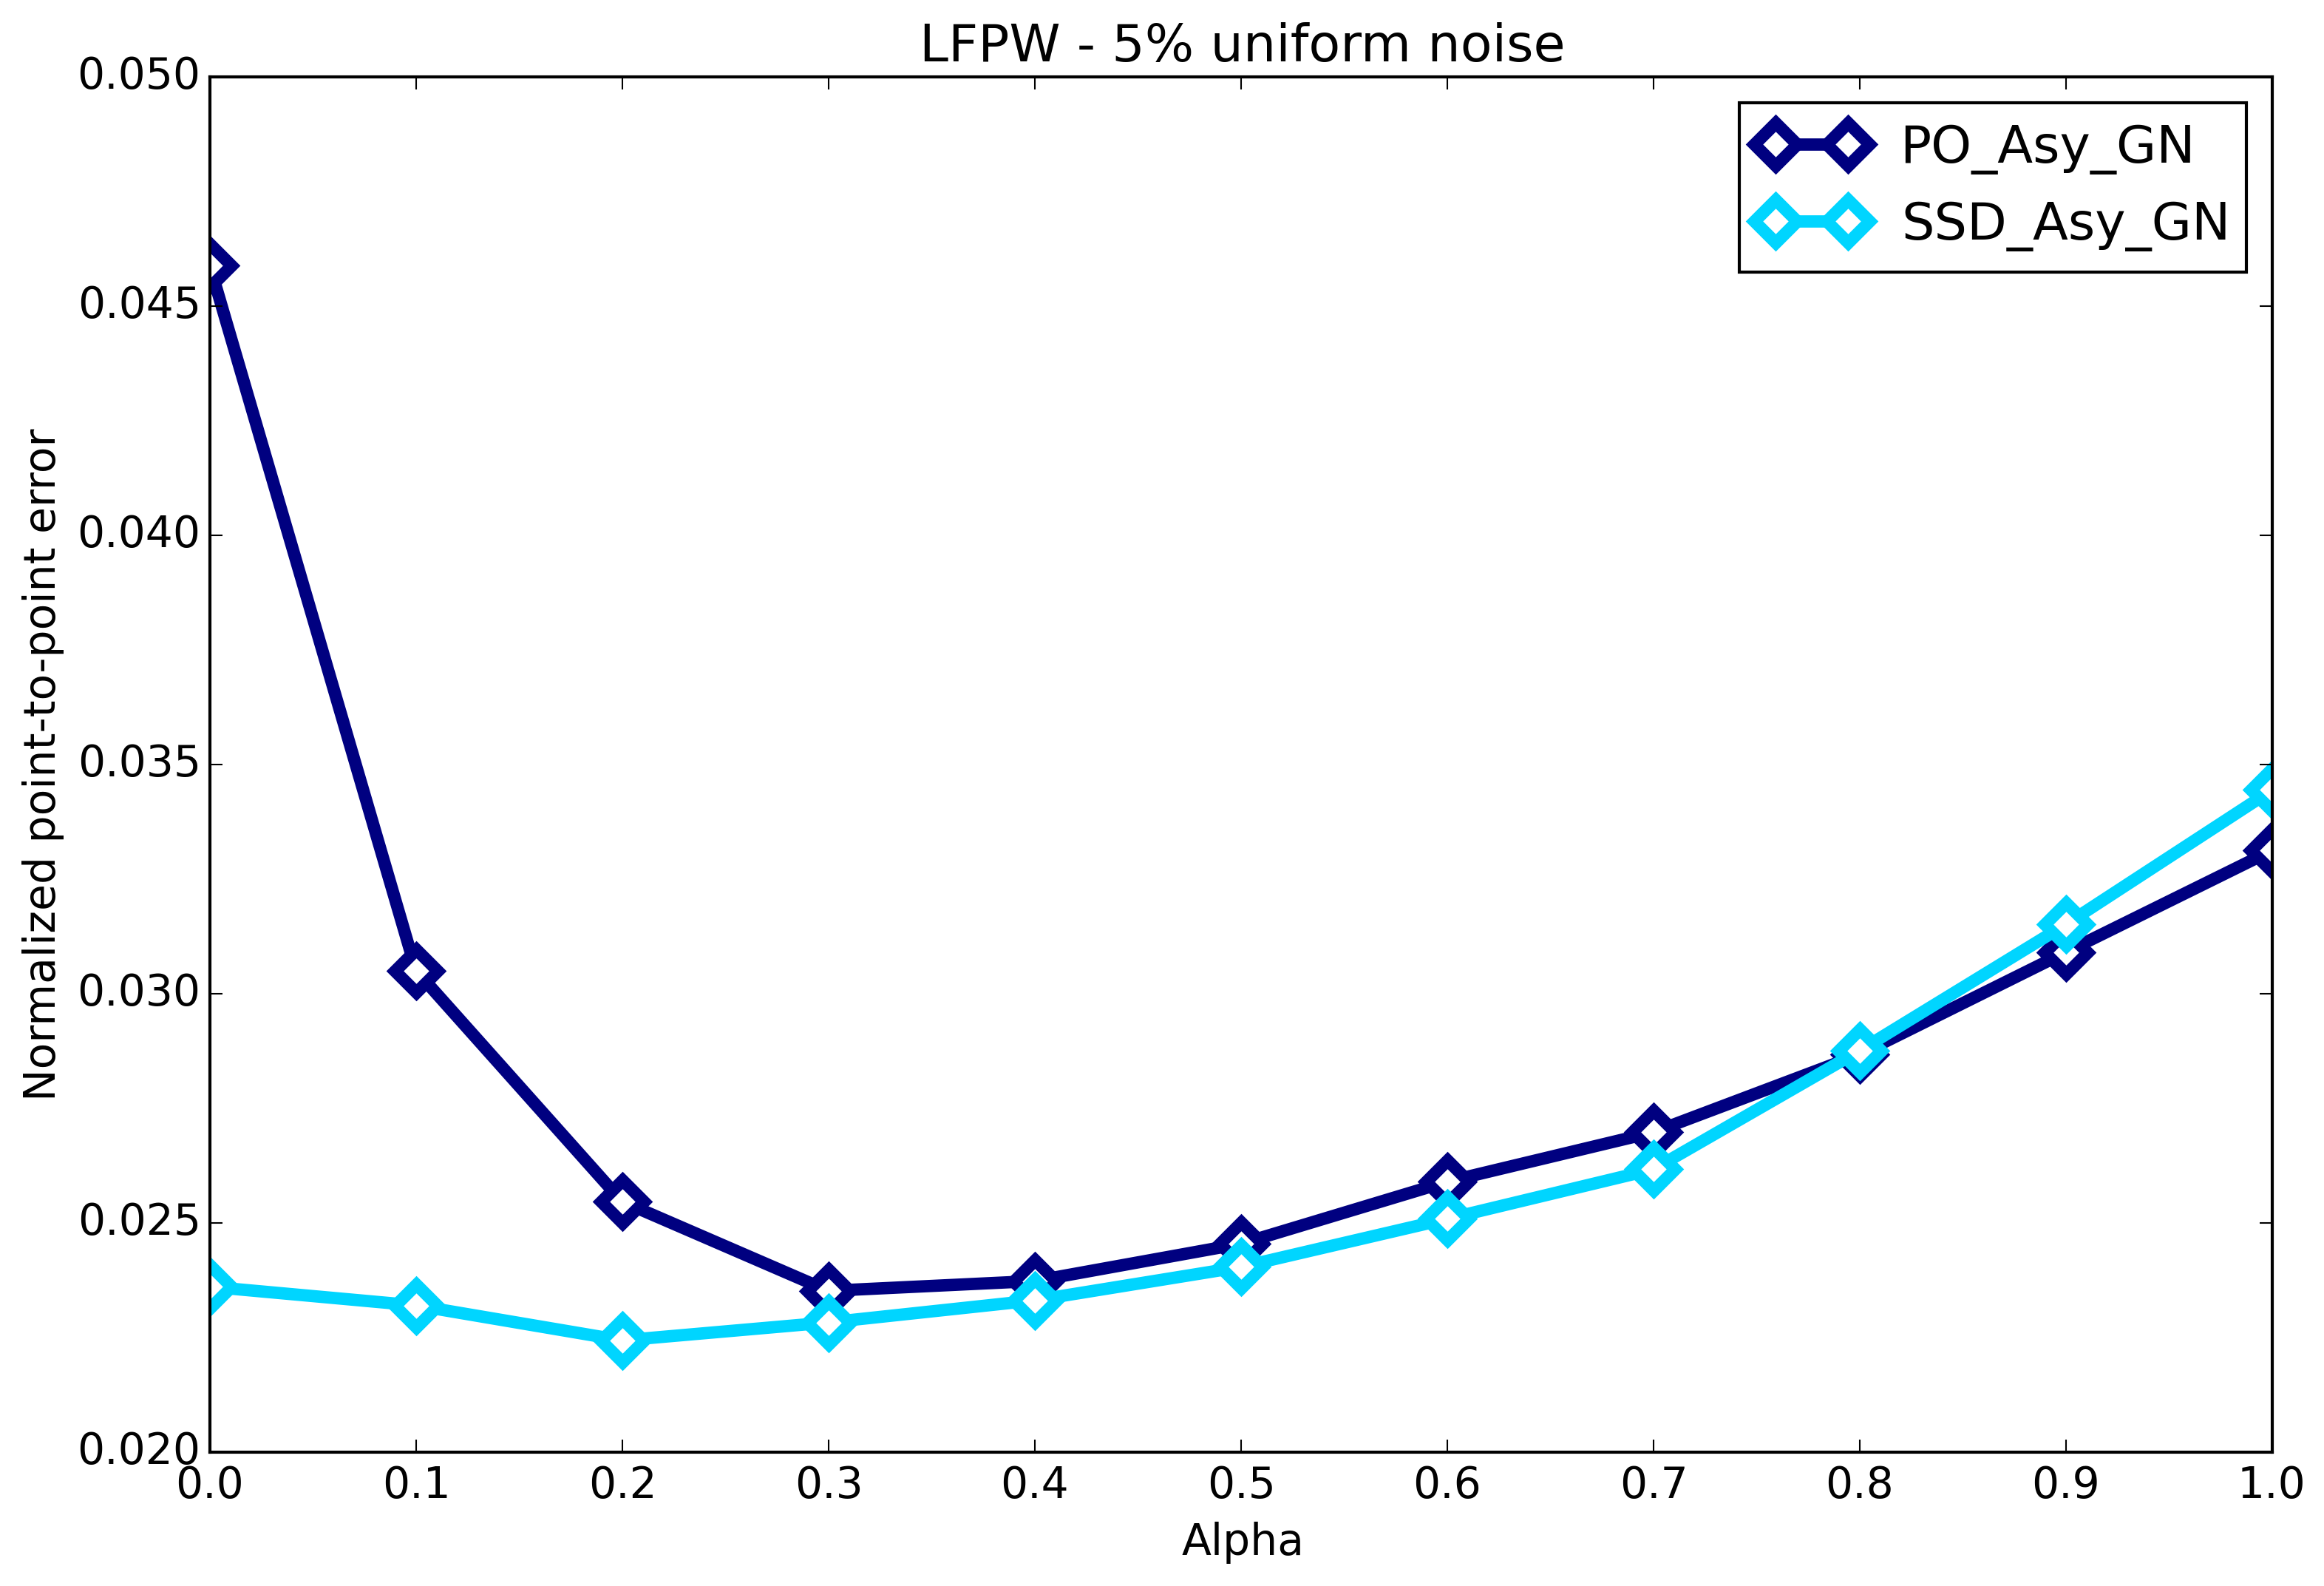
\includegraphics[width=0.48\textwidth]{experiments/alpha/mean_error_vs_alpha_asy_gn_5.png}
%     \caption{Mean normalized point-to-point error vs alpha on the LFPW test dataset for all Asymmetric Gauss-Newton algorithms initialized with $5\%$ uniform noise.}
%     \label{fig:alpha_5}
% \end{figure}


\subsubsection{Sampling}

\begin{figure*}[h!]
	\centering
	\begin{subfigure}{0.48\textwidth}
	    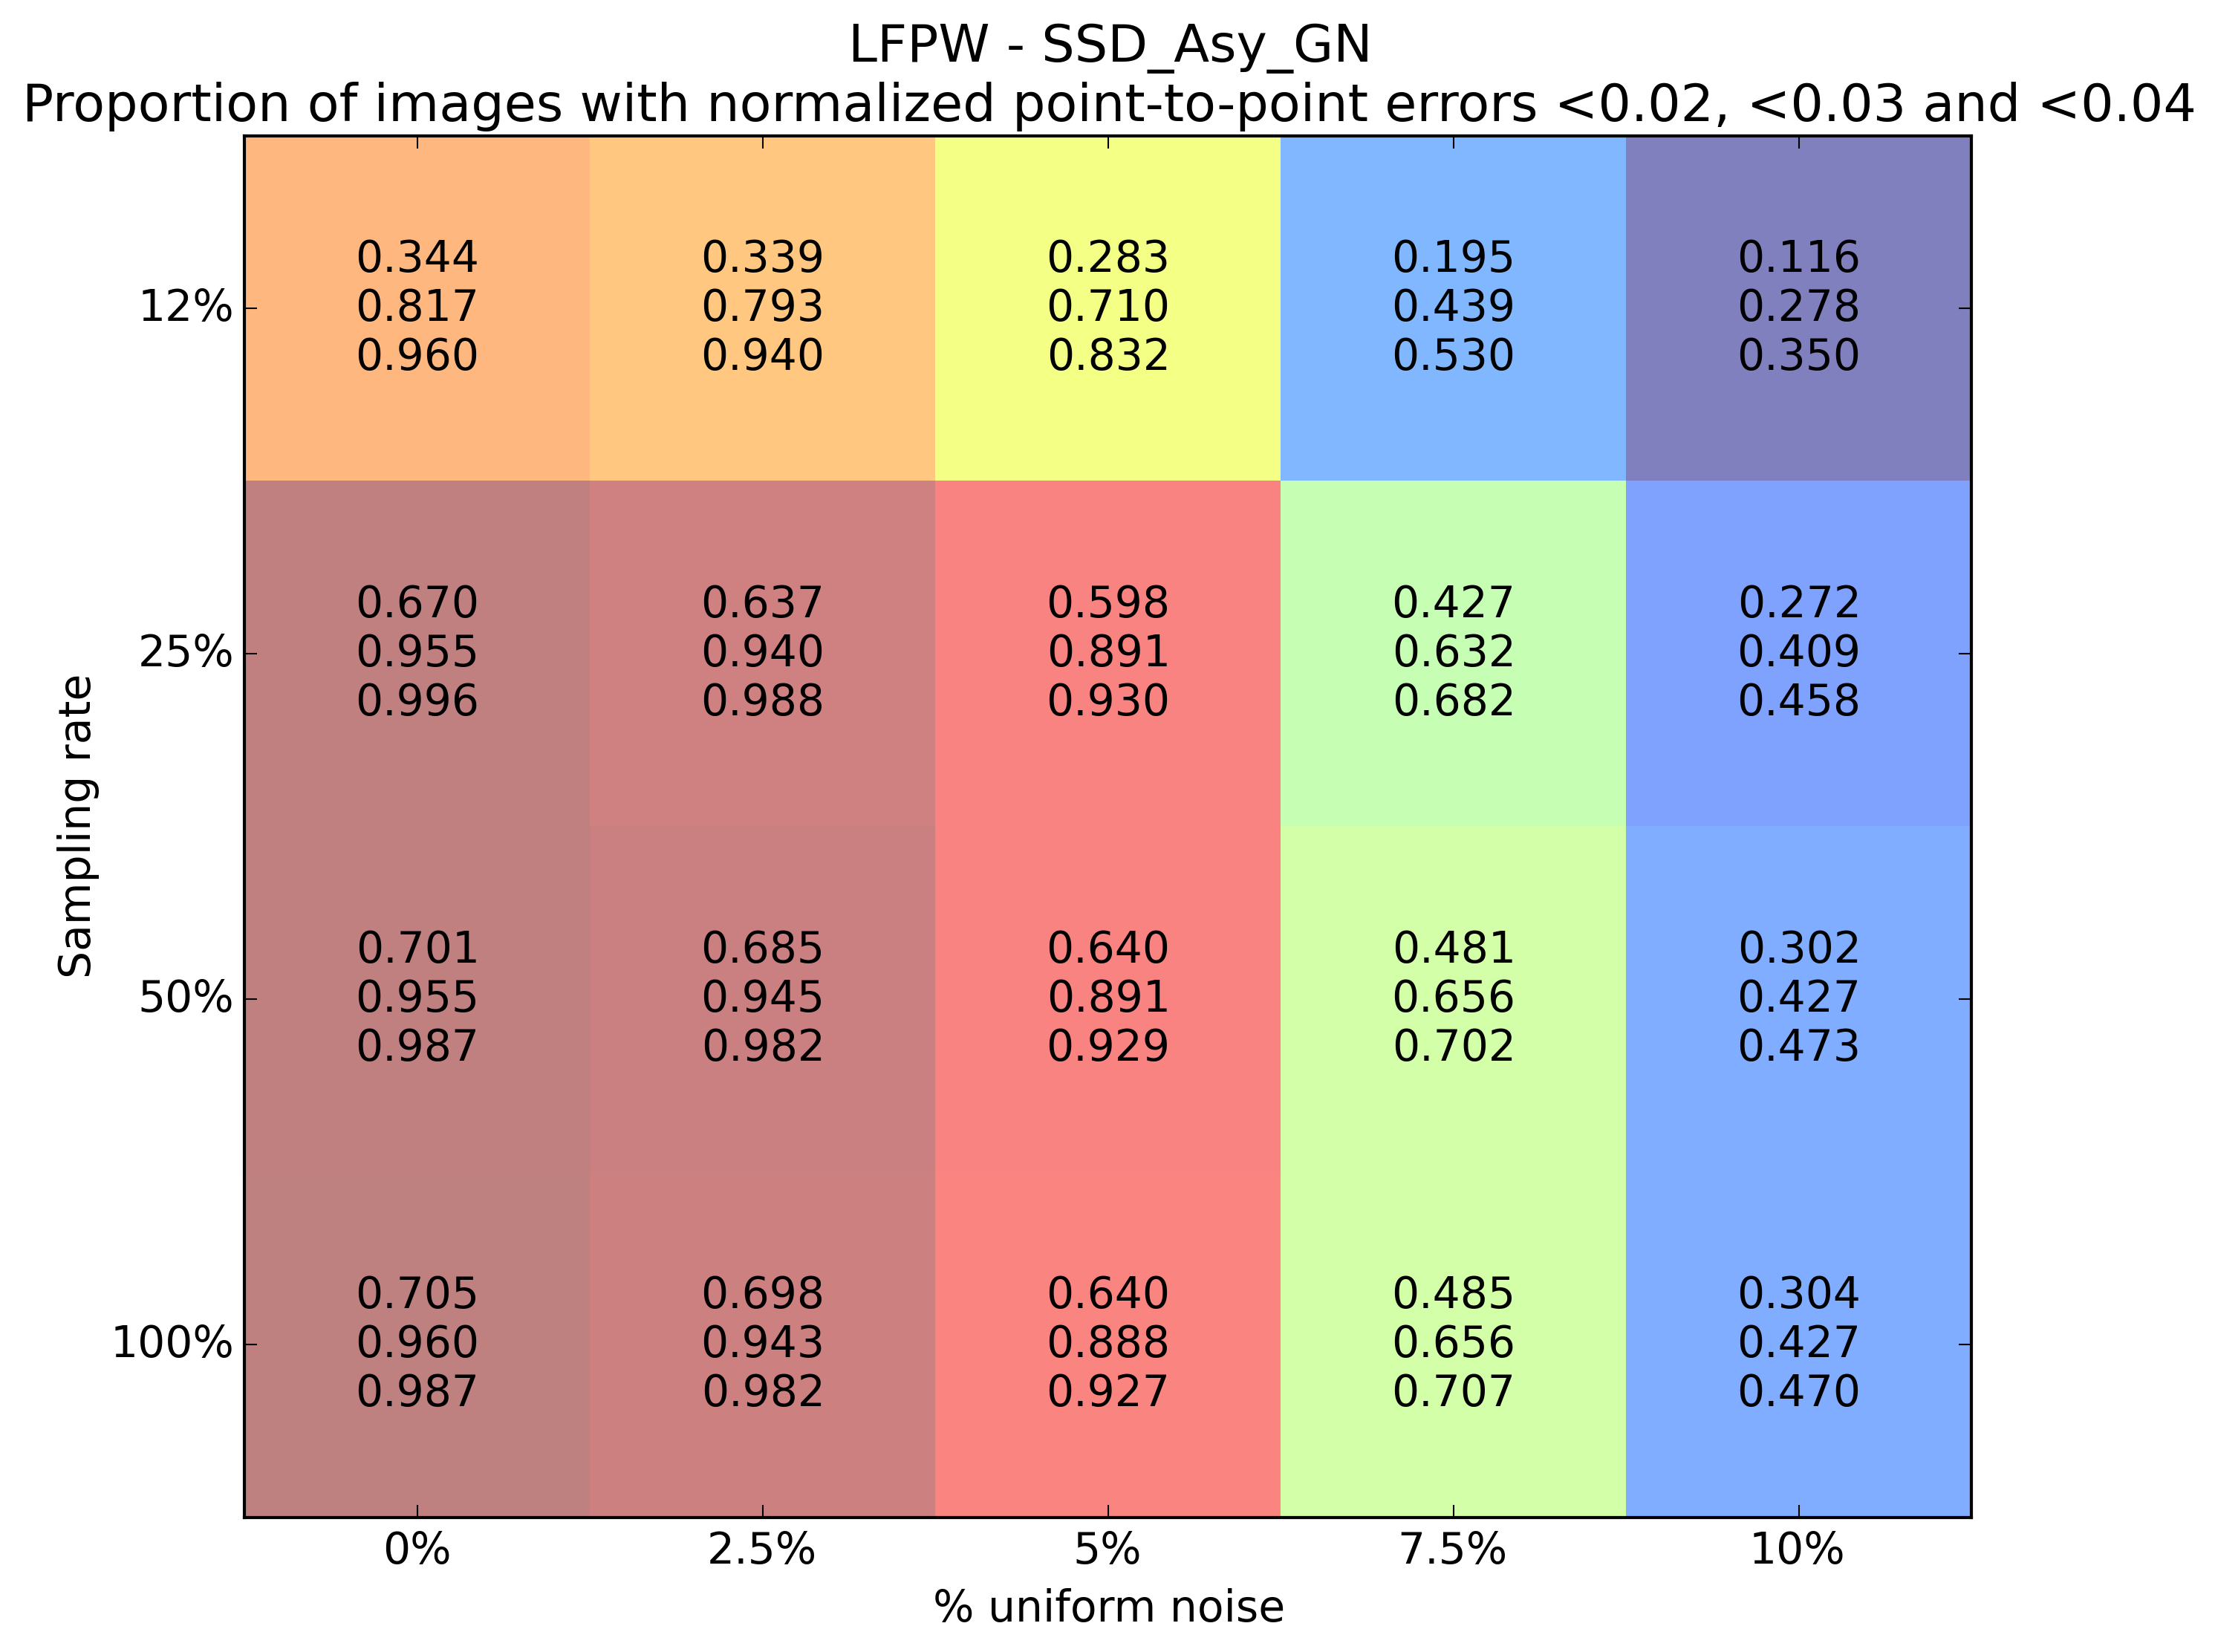
\includegraphics[width=\textwidth]{experiments/sampling/sampling_vs_noise_ssd_asy_gn.png}
	    \caption{Proportion of images with normalized point-to-point errors smaller than $0.02$, $0.03$ and $0.04$ for the SSD Asymmetric Gauss-Newton algorithm using different sampling rates and initialized with different amounts of noise.}
	    \label{fig:sampling_vs_noise_ssd_asy_gn}
	\end{subfigure}
	\hfill
	\begin{subfigure}{0.48\textwidth}
	    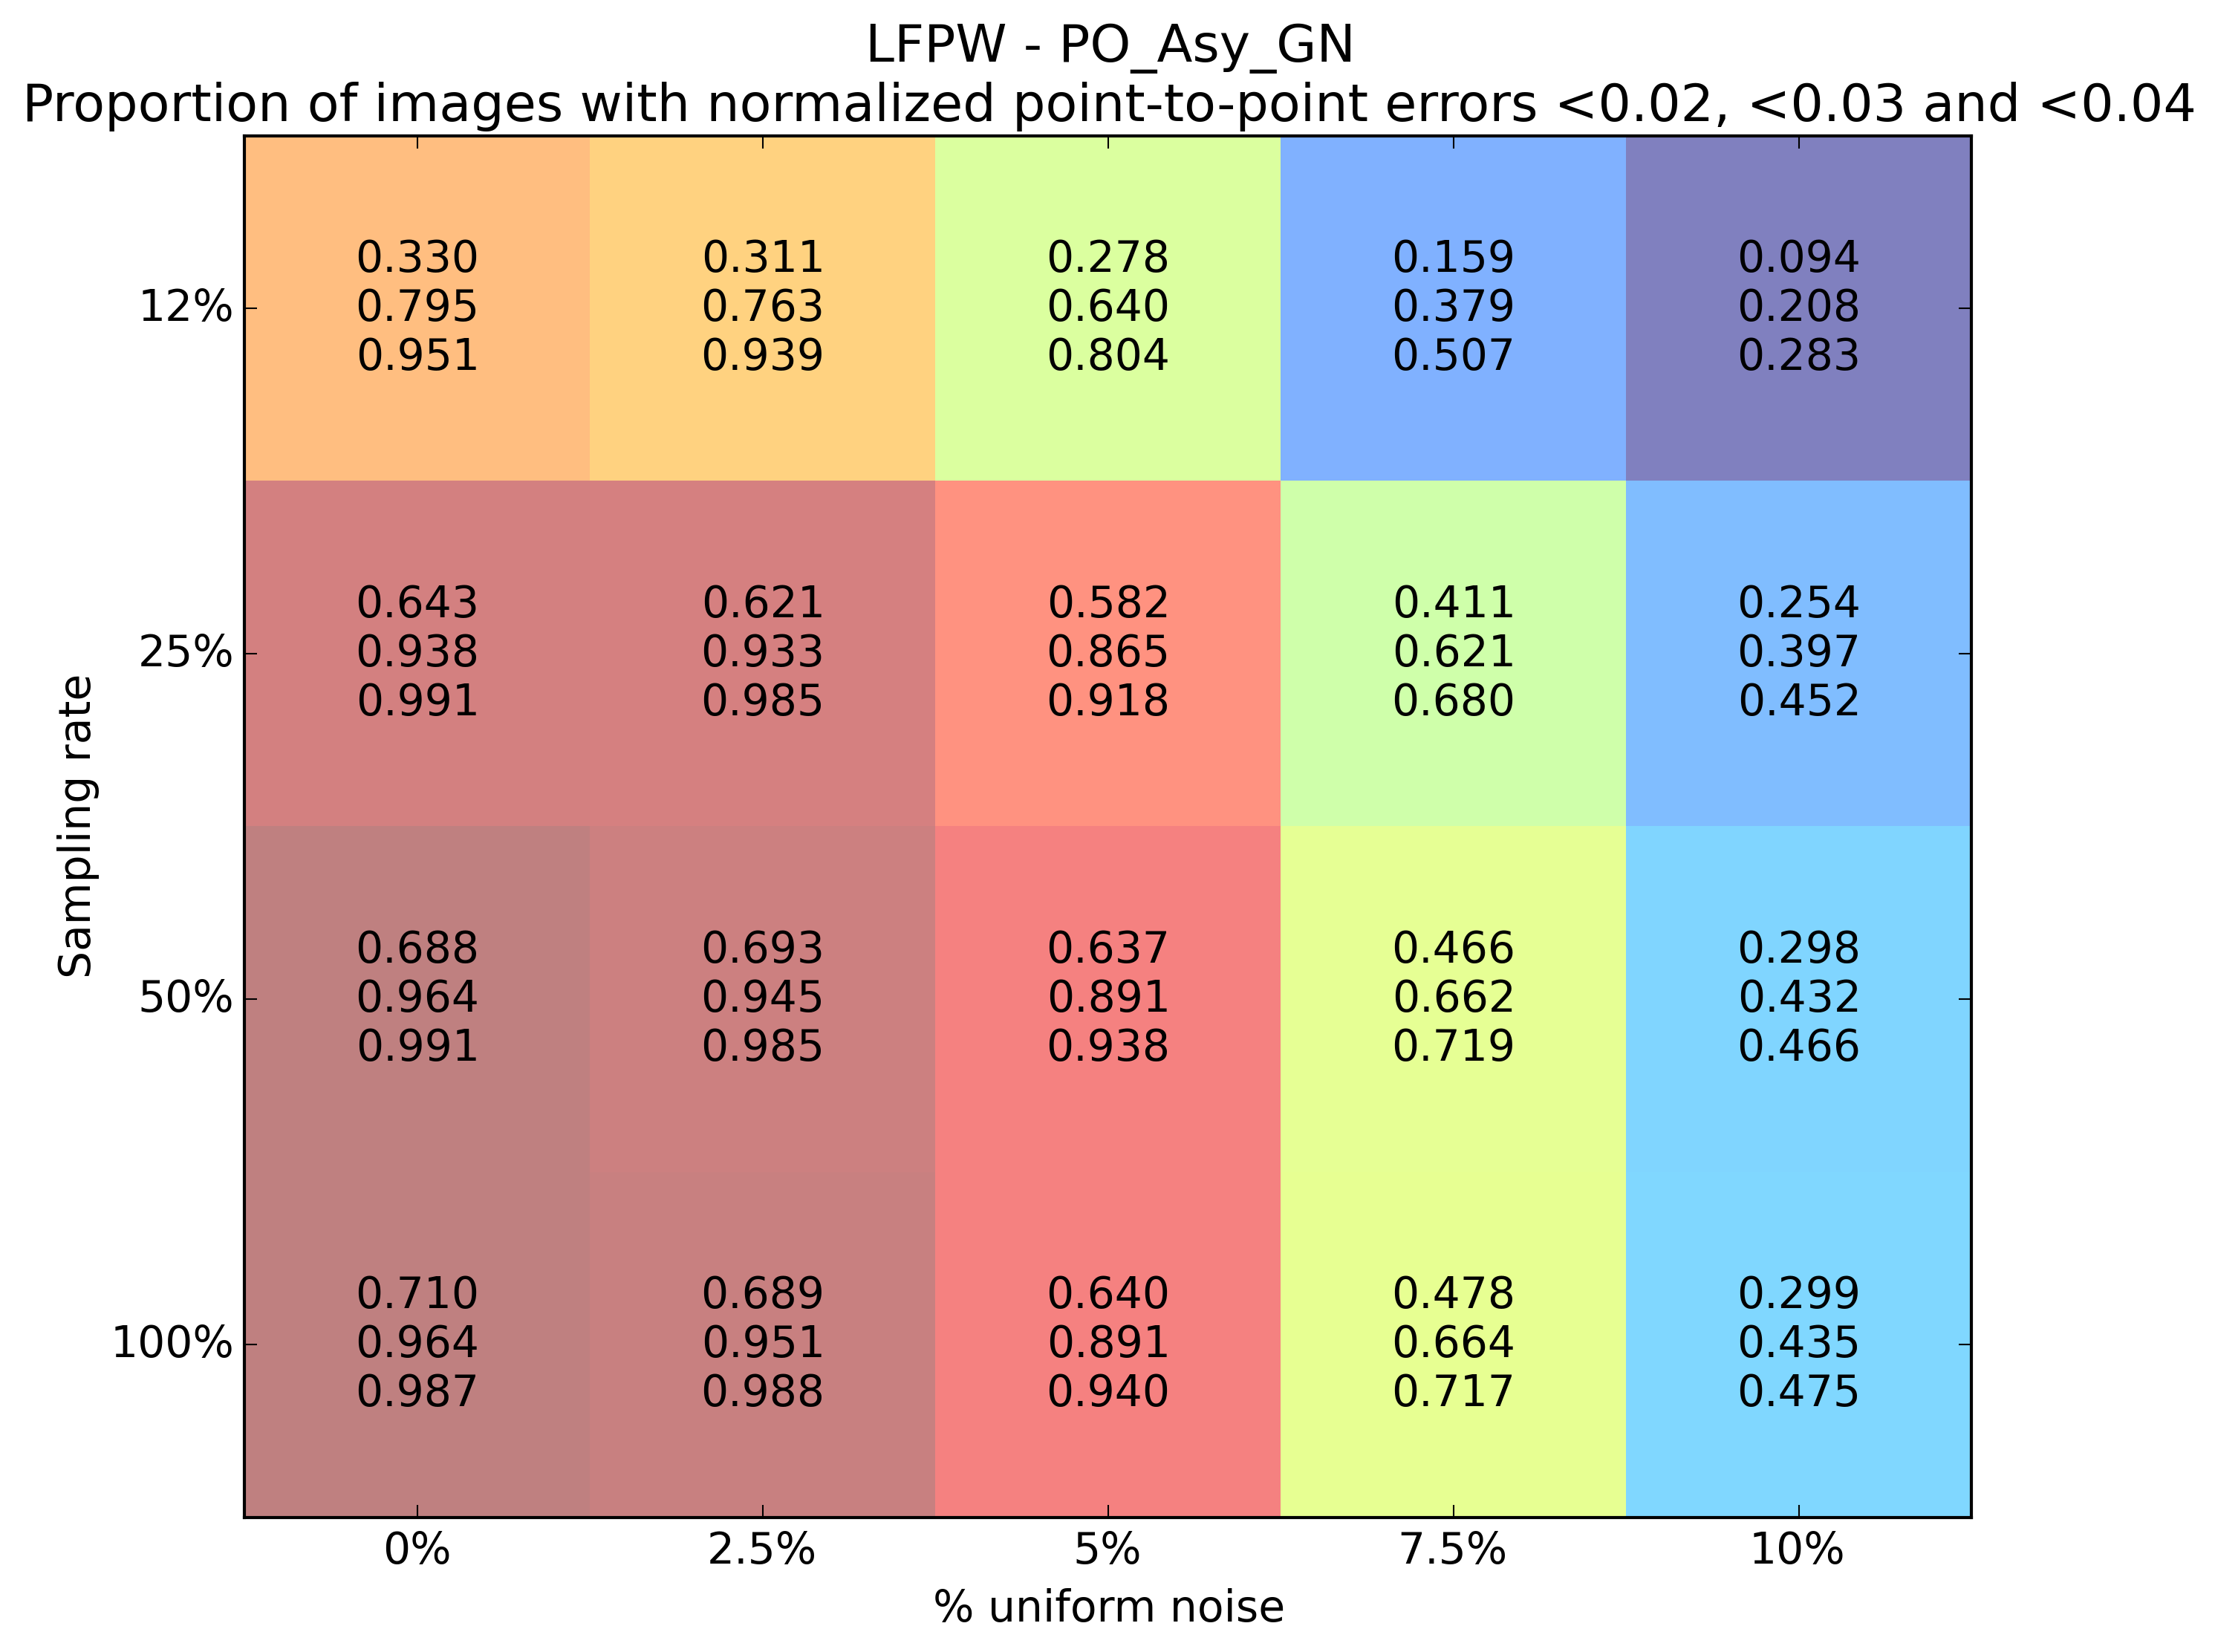
\includegraphics[width=\textwidth]{experiments/sampling/sampling_vs_noise_po_asy_gn.png}
	    \caption{Proportion of images with normalized point-to-point errors smaller than $0.02$, $0.03$ and $0.04$ for the Project-Out Asymmetric Gauss-Newton algorithm using different sampling rates and initialized with different amounts of noise.}
	    \label{fig:sampling_vs_noise_po_asy_gn}
	\end{subfigure}
	\label{fig:sampling}
	\caption{Results assessing the effectiveness of sampling for the best performing Project-Out and SSD algorithms on the LFPW database.}
\end{figure*}


\subsection{Comparison on Helen and AFW}

In this experiment, we report the fitting accuracy of the best performing CGD algorithms on the Helen database test set and on the entire AFW \cite{Zhu2012} database.

\begin{figure*}[h!]
	\centering
	\begin{subfigure}{0.48\textwidth}
	    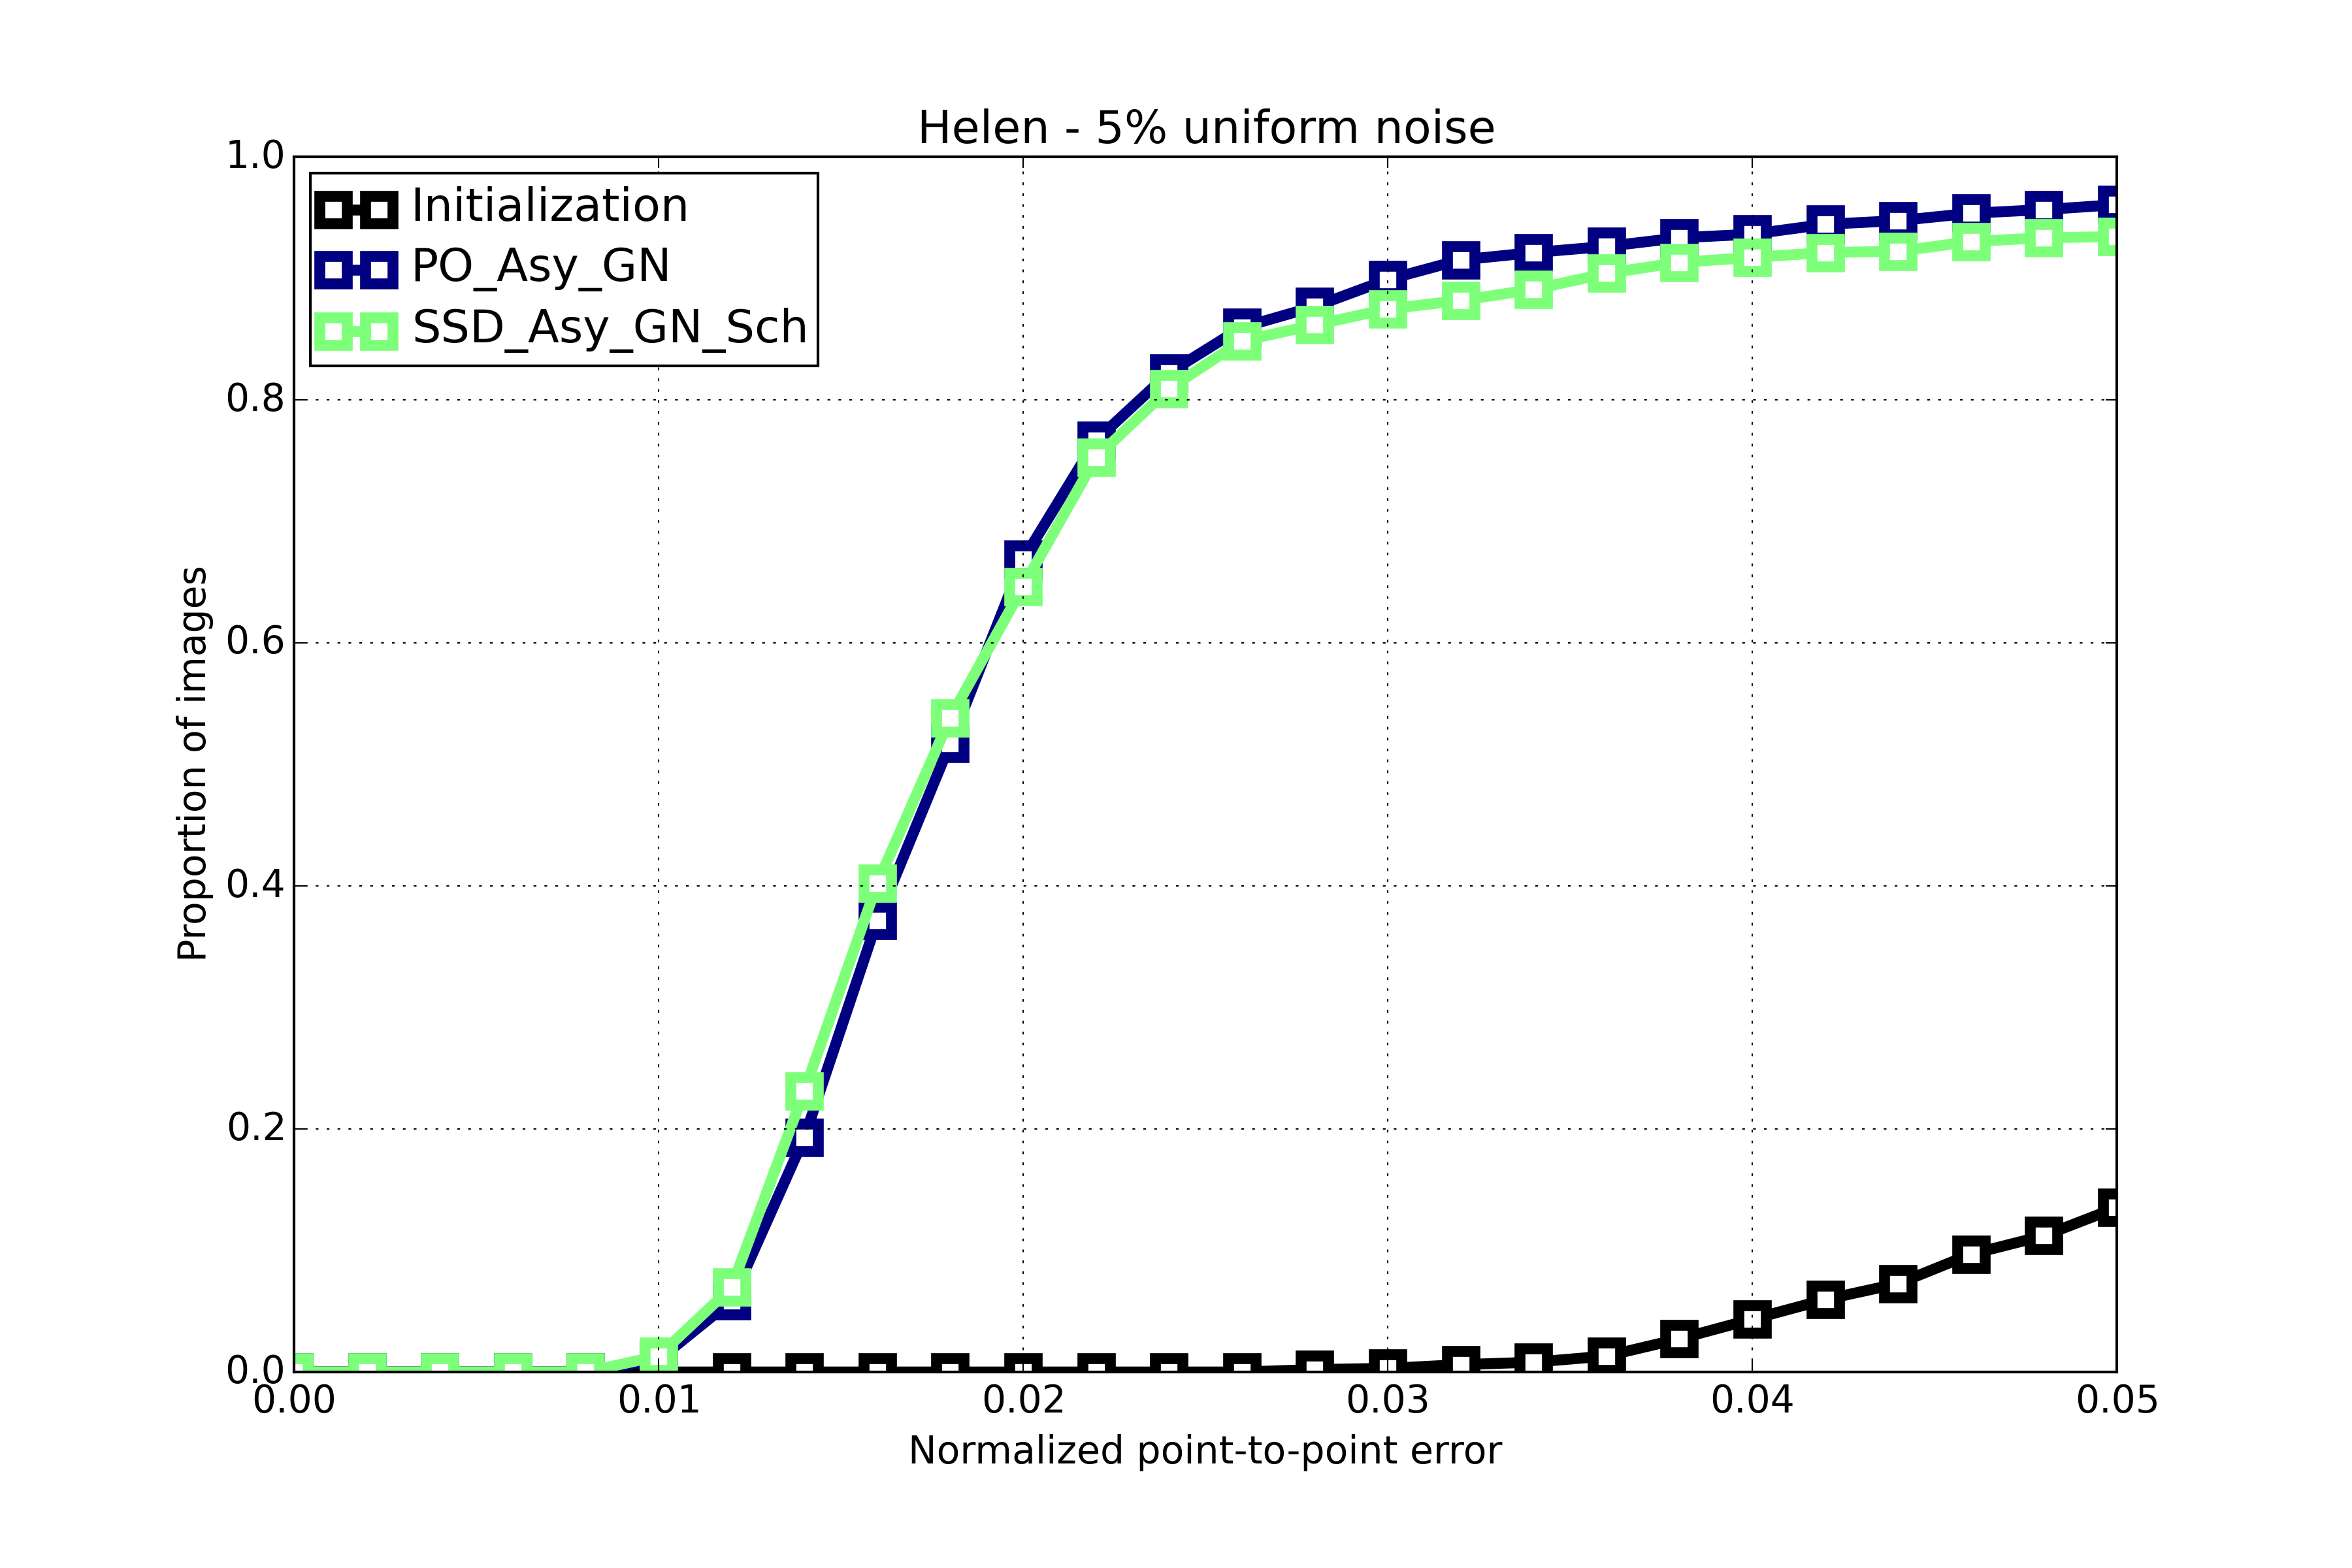
\includegraphics[width=\textwidth]{experiments/best/ced_helen_5.png}
	    \caption{CED on the Helen test dataset for the Project-Out and SSD Asymmetric Gauss-Newton algorithms initialized with $5\%$ noise.}
	    \label{fig:ced_po_for_gn}
	\end{subfigure}
	\hfill
	\begin{subfigure}{0.48\textwidth}
	    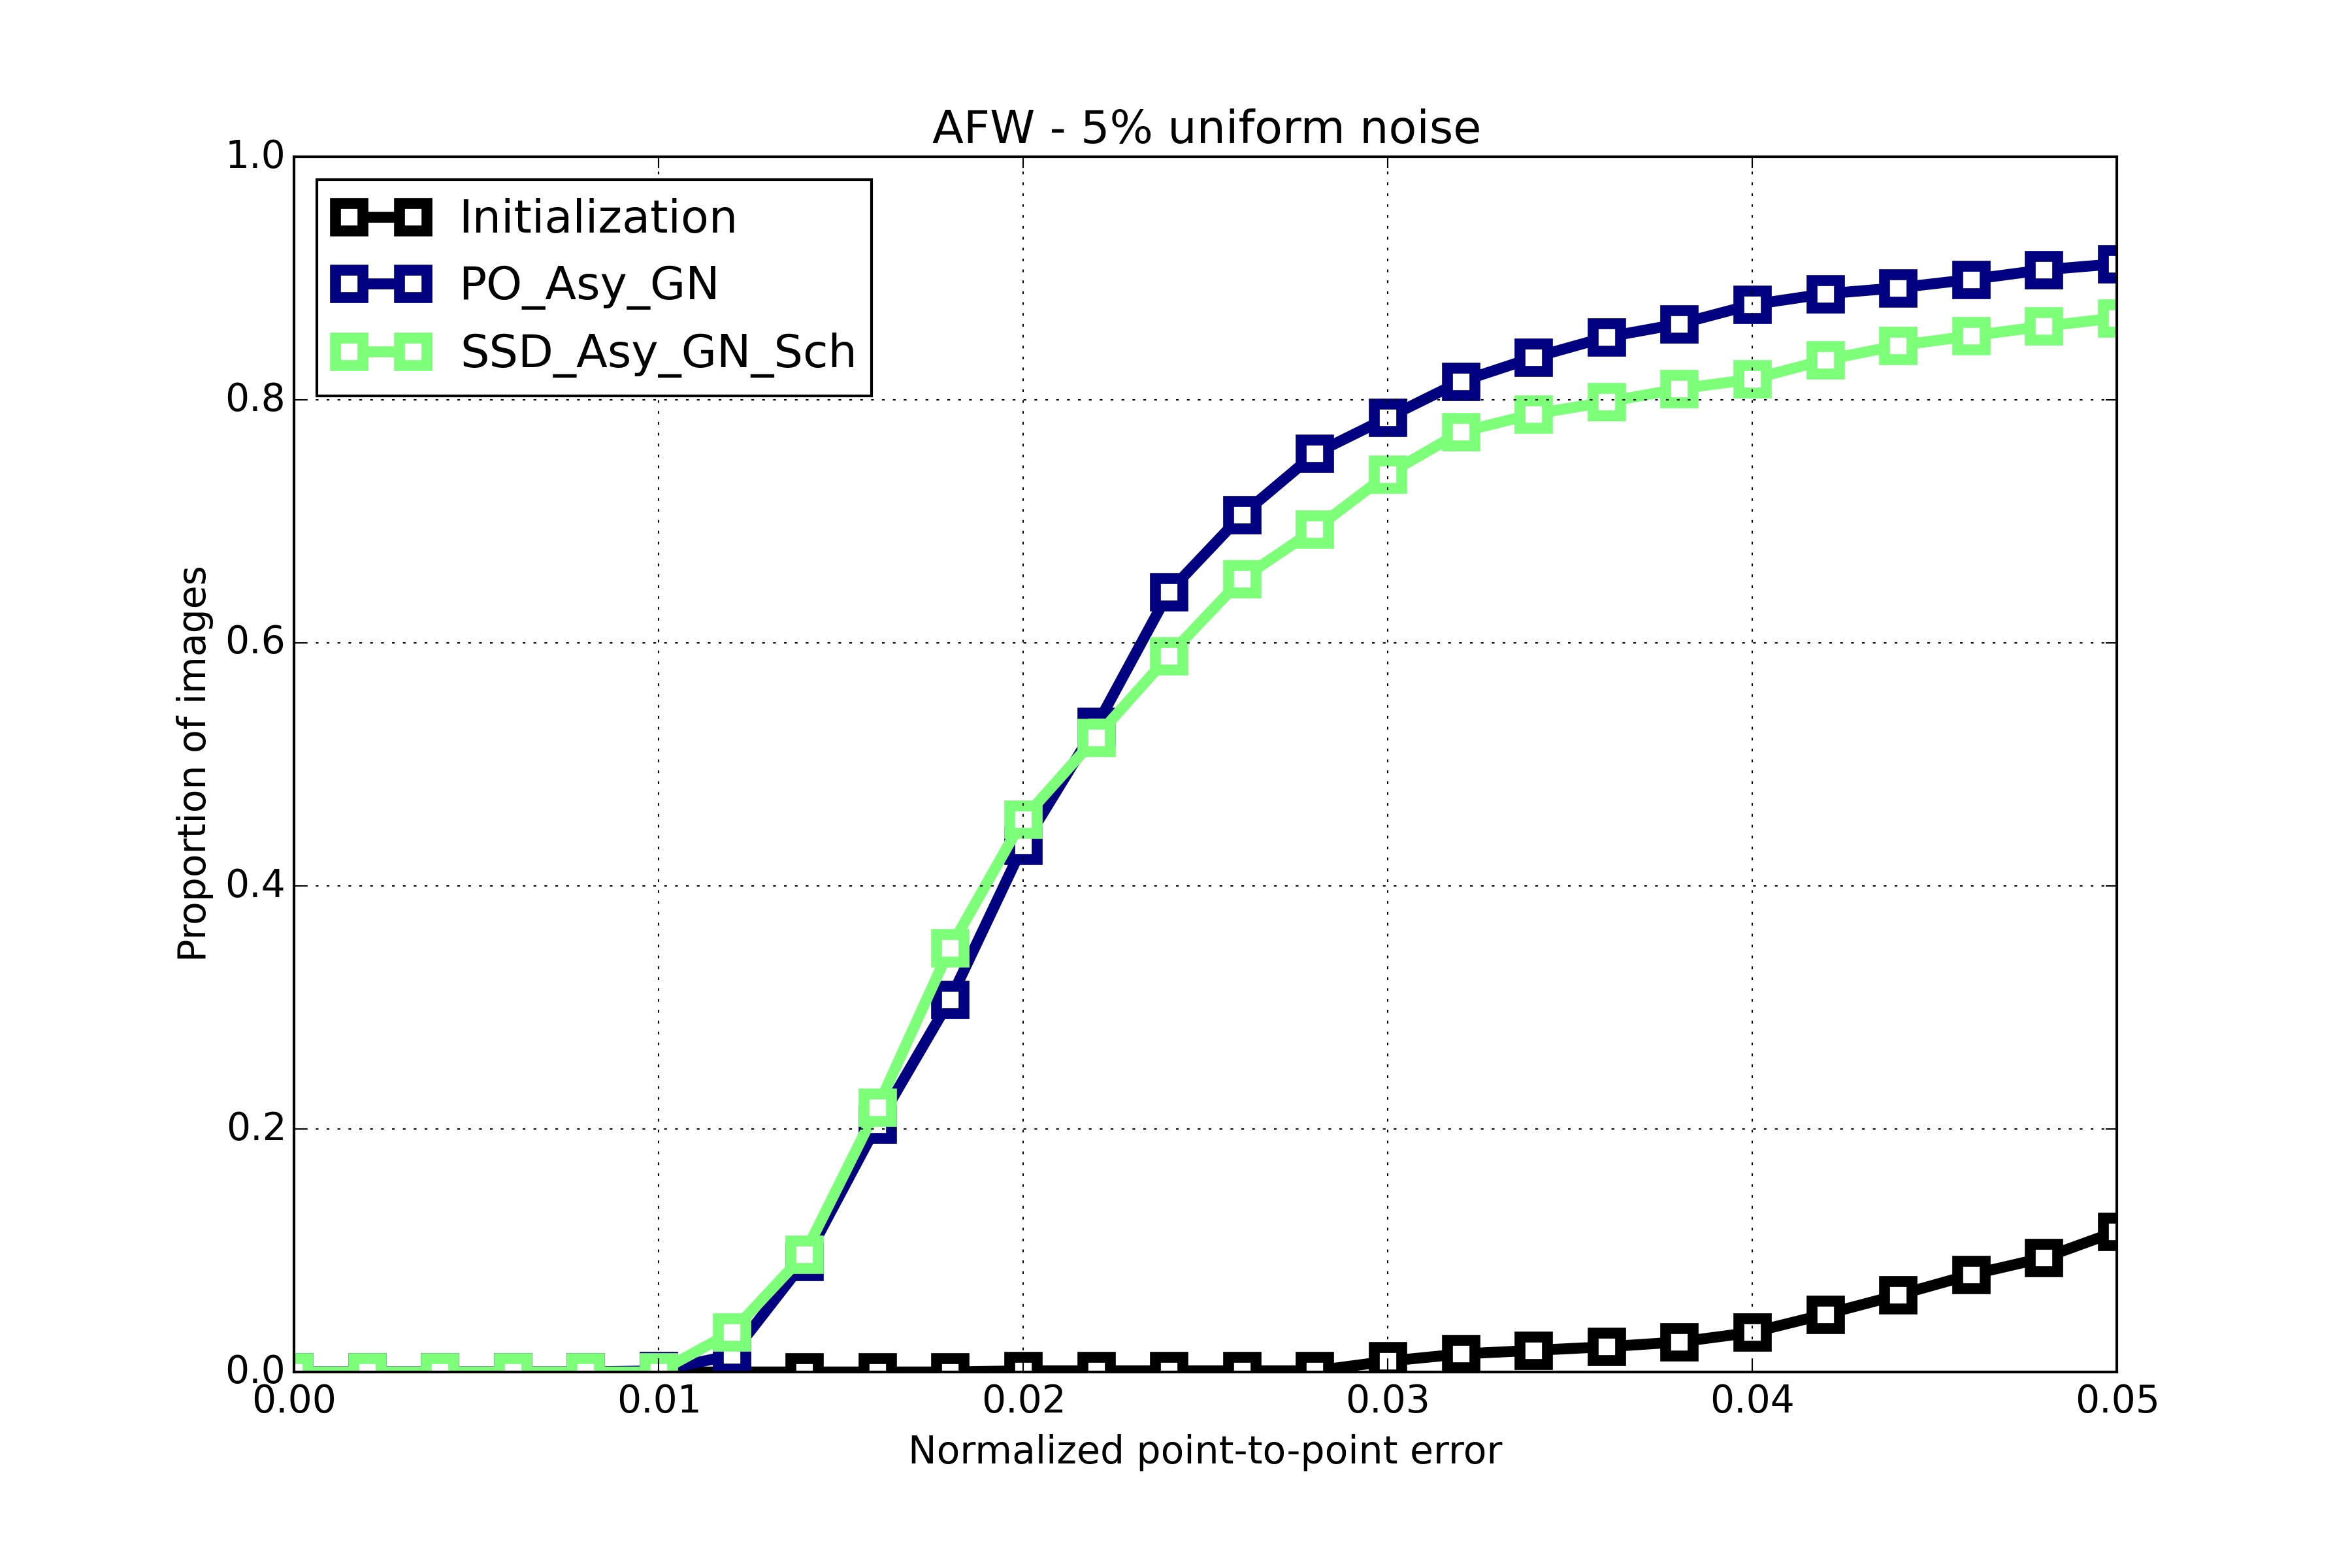
\includegraphics[width=\textwidth]{experiments/best/ced_afw_5.png}
	    \caption{CED on the AFW database for the Project-Out and SSD Asymmetric Gauss-Newton algorithm initialized with $5\%$ noise.}
	    \label{fig:ced_po_inv_gn}
	\end{subfigure}
	\label{fig:alpha}
	\caption{Results quantifying the effect of varying the value of the parameters $\alpha$ and $\beta$ in Asymmetric algorithms.}
\end{figure*}

% \begin{figure*}[h!]
% 	\centering
% 	\begin{subfigure}{0.48\textwidth}
% 	    \includegraphics[width=\textwidth]{experiments/best/helen/ced_best_5.png}
% 	    \caption{Cumulative Error Distribution on the entire AFW database for the best performing CGD algorithms initialized with $5\%$ uniform noise.}
% 	    \label{fig:helen_ced_best_5}
% 	\end{subfigure}
% 	\hfill
% 	\begin{subfigure}{0.48\textwidth}
% 		\includegraphics[width=\textwidth]{experiments/best/afw/ced_best_5.png}
% 	    \caption{Cumulative Error Distribution on the AFW database for the best performing CGD algorithms initialized with $5\%$ uniform noise.}
% 	    \label{fig:afw_ced_best_5}
% 	\end{subfigure}
% 	\label{fig:helen_afw}
% 	\caption{Experimental results on the Helen and AFW databases.}
% \end{figure*}


% \begin{figure*}[h!]
% 	\centering
% 	\begin{subfigure}{0.48\textwidth}
% 	    \includegraphics[width=\textwidth]{experiments/best/helen/ced_best_5.png}
% 	    \caption{Cumulative Error Distribution on the entire AFW database for the best performing CGD algorithms initialized with $5\%$ uniform noise.}
% 	    \label{fig:helen_ced_best_5}
% 	\end{subfigure}
% 	\hfill
% 	\begin{subfigure}{0.48\textwidth}
% 	    \includegraphics[width=\textwidth]{experiments/best/helen/mean_error_vs_iters_best_5.png}
% 	    \caption{Mean normalized point-to-point error vs number of iterations on the entire AFW database for the best performing CGD algorithms initialized with $5\%$ uniform noise.}
% 	    \label{fig:helen_mean_error_vs_iters_best_5}
% 	\end{subfigure}
% 	\par\medskip
% 	\begin{subfigure}{0.48\textwidth}
% 	    \includegraphics[width=\textwidth]{experiments/best/helen/mean_cost_vs_iters1_best_5.png}
% 	    \caption{Mean normalized cost vs number of first pyramid level iterations on the entire AFW database for the best performing CGD algorithms initialized with $5\%$ uniform noise.}
% 	    \label{fig:helen_mean_cost_vs_iters1_best_5}
% 	\end{subfigure}
% 	\hfill
% 	\begin{subfigure}{0.48\textwidth}
% 	    \includegraphics[width=\textwidth]{experiments/best/helen/mean_cost_vs_iters2_best_5.png}
% 	    \caption{Mean normalized cost vs number of first pyramid level iterations on the entire AFW database for the best performing CGD algorithms initialized with $5\%$ uniform noise..}
% 	    \label{fig:helen_mean_cost_vs_iters2_best_5}
% 	\end{subfigure}
% 	\label{fig:helen}
% 	\caption{Experimental results on the Helen database.}
% \end{figure*}


% \begin{figure*}[h!]
% 	\centering
% 	\begin{subfigure}{0.48\textwidth}
% 	    \includegraphics[width=\textwidth]{experiments/best/afw/ced_best_5.png}
% 	    \caption{Cumulative Error Distribution on the AFW database for the best performing CGD algorithms initialized with $5\%$ uniform noise.}
% 	    \label{fig:afw_ced_best_5}
% 	\end{subfigure}
% 	\hfill
% 	\begin{subfigure}{0.48\textwidth}
% 	    \includegraphics[width=\textwidth]{experiments/best/afw/mean_error_vs_iters_best_5.png}
% 	    \caption{Mean normalized point-to-point error vs number of iterations on the AFW database for the best performing CGD algorithms initialized with $5\%$ uniform noise.}
% 	    \label{fig:afw_mean_error_vs_iters_best_5}
% 	\end{subfigure}
% 	\par\medskip
% 	\begin{subfigure}{0.48\textwidth}
% 	    \includegraphics[width=\textwidth]{experiments/best/afw/mean_cost_vs_iters1_best_5.png}
% 	    \caption{Mean normalized cost vs number of first pyramid level iterations on the AFW database for the best performing CGD algorithms initialized with $5\%$ uniform noise.}
% 	    \label{fig:afw_mean_cost_vs_iters1_best_5}
% 	\end{subfigure}
% 	\hfill
% 	\begin{subfigure}{0.48\textwidth}
% 	    \includegraphics[width=\textwidth]{experiments/best/afw/mean_cost_vs_iters2_best_5.png}
% 	    \caption{Mean normalized cost vs number of first pyramid level iterations on the AFW database for the best performing CGD algorithms initialized with $5\%$ uniform noise..}
% 	    \label{fig:afw_mean_cost_vs_iters2_best_5}
% 	\end{subfigure}
% 	\label{fig:afw}
% 	\caption{Experimental results on the AFW database.}
% \end{figure*}



% This section reports the performance of the proposed method on the problem of face alignment in-the-wild. Results for two different experiments are reported. The first experiment compares the accuracy and convergence properties of the proposed Unified PIC-RLMS and AIC-RLMS algorithms with respect to those of PIC \cite{Baker2004}, AIC \cite{Papandreou2008} and and RLMS \cite{Saragih2011} on the popular LFPW \cite{Belhumeur2011} and Helen \cite{Le2012} datasets. The second experiment compares the performance of the previous algorithms against recently proposed state-of-the-art methods for face alignment in-the-wild, \ie the Supervised Descent Method of Xiong and De La Torre \cite{Xiong2013} and the Gauss-Newton Deformable Parts Model of Tzimiropoulos and Pantic \cite{Tzimiropoulos2014}, on the very challenging Annotated Faces in the Wild (AFW) dataset.

% \subsection{Comparison with AAMs and CLMs}
% Results for this experiment are reported over the 224 and 330 test images of the LFPW \cite{Belhumeur2011} and Helen\cite{Le2012} datasets. 66 points ground truth landmark annotations were provided by the iBUG group\footnote{\label{ibug_300}\url{http://ibug.doc.ic.ac.uk/resources/300-W/}}. All methods were initialized by perturbing the ground truth scale and translation parameters with Gaussian noise (rotations were not considered) and applying the resulting transformation to mean of the shape model. (Notice that this procedure produces initializations that are considerably more challenging than those reported in the recent AAM literature \cite{Tzimiropoulos2013, Tzimiropoulos2014}). The Cumulative Error Distributions (CED) for this experiment is shown in Figures \ref{fig:lfpw_exp1} and \ref{fig:helen_exp1}. Figures \ref{fig:lfpw_exp2} and \ref{fig:helen_exp2} shows the evolution of the mean normalized point-to-point error as a function of the number of iterations run by each algorithm. This experiment shows that our Unified AIC-RLMS approach considerably outperforms all other methods by a large margin on both datasets. More specifically, AIC-RLMS achieves a constant improvement of between 10\% to 20\% over PIC-RLMS and AIC at the significant region $0.020 < err > 0.040$ (at which the results are generally considered adequate by visual inspection). Note that the fast Unified PIC-RLMS algorithm is also the second most performant algorithm, surpassing both AIC and RLMS, on this particular experiment.

% \subsection{Comparison with state of the art}

% Results for this experiment are reported over the 337 images of the AFW \cite{Zhu2012} dataset. In this case, 49 points ground truth landmark annotations for this dataset were again provided by the iBUG group\footnoteref{ibug_300}. Results for \cite{Xiong2013} and \cite{Tzimiropoulos2014} were directly obtained using the publicly available models and fitting code kindly provided by the authors\footnote{\url{http://www.humansensing.cs.cmu.edu/intraface/}}$^{,}$\footnote{\url{http://ibug.doc.ic.ac.uk/resources/gauss-newton-deformable-part-models-face-alignment/}}. Note that, the provided models have been potentially trained using thousands of images in contrast to the only 813 images used to trained our method. In this experiment, all algorithms were initialized using the bounding box provided by our own in-house implementation of the face detector of \cite{Zhu2012}. The CED for this experiment are reported in Figure \ref{fig:afw_exp}. The results show that our Unified AIC-RLMS algorithm achieves state-of-the-art results on the AFW dataset, considerably outperforming both the Gauss-Newton Deformable Parts-Model of Tzimiropoulos and Pantic \cite{Tzimiropoulos2014} (which can be extremely accurate but sensitive to inaccurate initializations) and the SDM method of Xiong and De la Torre \cite{Xiong2013} (which can deal with very noisy initializations but is significantly less accurate than our method).

% \begin{figure}[t!]
% \centering
% \includegraphics[width=0.38\textwidth]{figures/graph7.png}
% \caption{Cumulative Error Distributions over 49 landmarks for the AFW dataset.}
% \label{fig:afw_exp}
% \end{figure}


\begin{table*}
\begin{tabular}{lc}
\hline\noalign{\smallskip}
Gauss-Newton algorithms & Computational cost
\\
\noalign{\smallskip}
\hline
\noalign{\smallskip}
PO\_For\_GN \cite{Amberg2009, Tzimiropoulos2013} & $O(
               \underbrace{nF}_{\mathbf{J}_\mathbf{i}}
               +
               \underbrace{mnF}_{\mathbf{J}_\mathbf{i}^T\bar{\mathbf{A}}}
               +
               \underbrace{n^2F}_{\mathbf{J}_\mathbf{i}^T\bar{\mathbf{A}}\mathbf{J}_\mathbf{i}}
               +
               \underbrace{n^3}_{\mathbf{H}_\mathbf{i}^{-1}}
               +
               \underbrace{nF}_{\mathbf{J}_\mathbf{i}^T\bar{\mathbf{A}}\mathbf{r}}
               +
               \underbrace{n^2}_{(\mathbf{J}_\mathbf{i}^T\bar{\mathbf{A}}\mathbf{J}_\mathbf{i})^{-1}\mathbf{J}_\mathbf{i}^T\bar{\mathbf{A}}\mathbf{r}}$
               )
\\
\noalign{\smallskip}
% \hline
\noalign{\smallskip}
PO\_Inv\_GN \cite{Matthews2004} & $O(
               \underbrace{nF}_{\mathbf{H}_{\bar{\mathbf{a}}}^{-1}\mathbf{J}_{\bar{\mathbf{a}}}^T\bar{\mathbf{A}}\mathbf{r}}$
               )
\\
\noalign{\smallskip}
% \hline
\noalign{\smallskip}
PO\_Asy\_GN & $O(
               \underbrace{nF}_{\mathbf{J}_\mathbf{i}}
               +
               \underbrace{mnF}_{\mathbf{J}_\mathbf{t}^T\bar{\mathbf{A}}}
               +
               \underbrace{n^2F}_{\mathbf{J}_\mathbf{t}^T\bar{\mathbf{A}}\mathbf{J}_\mathbf{t}}
               +
               \underbrace{n^3}_{\mathbf{H}_\mathbf{t}^{-1}}
               +
               \underbrace{nF}_{\mathbf{J}_\mathbf{t}^T\bar{\mathbf{A}}\mathbf{r}}
               +
               \underbrace{n^2}_{\mathbf{H}_\mathbf{t}^{-1}\mathbf{J}_\mathbf{t}^T\bar{\mathbf{A}}\mathbf{r}}$
               )
\\
\noalign{\smallskip}
% \hline
\noalign{\smallskip}
PO\_Bid\_GN\_Sch & $O(
               \underbrace{nF}_{\mathbf{J}_\mathbf{i}}
               +
               \underbrace{mnF}_{\mathbf{J}_{\bar{\mathbf{a}}}^T\mathbf{P} \, \& \,  \mathbf{J}_\mathbf{i}^T\bar{\mathbf{A}}}
               +
               \underbrace{n^2F}_{\mathbf{J}_{\bar{\mathbf{a}}}^T\mathbf{P}\mathbf{J}_{\bar{\mathbf{a}}} \, \& \,  \mathbf{J}_\mathbf{i}^T\bar{\mathbf{A}}\mathbf{J}_\mathbf{i}}
               +
               \underbrace{n^3}_{\mathbf{H}_{\bar{\mathbf{a}}}^{-1} \, \& \,  \mathbf{H}_\mathbf{i}^{-1}}
               +
               \underbrace{2nF}_{\mathbf{J}_{\bar{\mathbf{a}}}^T\mathbf{P}\mathbf{r} \, \& \,  \mathbf{J}_\mathbf{i}^T\bar{\mathbf{A}}\mathbf{r}}
               +
               \underbrace{2n^2}_{\mathbf{H}_{\bar{\mathbf{a}}}^{-1}\mathbf{J}_{\bar{\mathbf{a}}}^T\mathbf{P}\mathbf{r} \, \& \,  \mathbf{H}_\mathbf{i}^{-1}\mathbf{J}_\mathbf{i}^T\bar{\mathbf{A}}\mathbf{r}}$
               )
\\
\noalign{\smallskip}
% \hline
\noalign{\smallskip}
PO\_Bid\_GN\_Alt & $O(
               \underbrace{nF}_{\mathbf{J}_\mathbf{i}}
               +
               \underbrace{mnF}_{\mathbf{J}_\mathbf{i}^T\bar{\mathbf{A}}}
               +
               \underbrace{n^2F}_{\mathbf{J}_\mathbf{i}^T\bar{\mathbf{A}}\mathbf{J}_\mathbf{i}}
               +
               \underbrace{n^3}_{\mathbf{H}_\mathbf{i}^{-1}}
               +
               \underbrace{2nF}_{\mathbf{H}_{\bar{\mathbf{a}}}^{-1}\mathbf{J}_{\bar{\mathbf{a}}}^T\mathbf{r} \, \& \,\mathbf{J}_\mathbf{i}^T\bar{\mathbf{A}}\mathbf{r}}
               +
               \underbrace{2n^2}_{\mathbf{H}_{\bar{\mathbf{a}}}^{-1}\mathbf{J}_{\bar{\mathbf{a}}}^T\mathbf{P}\mathbf{r} \, \& \, \mathbf{H}_\mathbf{i}^{-1}\mathbf{J}_\mathbf{i}^T\mathbf{r}}$
               )
\\
\noalign{\smallskip}
% \hline
\noalign{\smallskip}
SSD\_For\_GN\_Sch \cite{Amberg2009, Tzimiropoulos2013} & $O(
			   \underbrace{mF}_{\mathbf{A}^T\mathbf{r}}
			   +
			   \underbrace{nF}_{\mathbf{J}_\mathbf{i}}
               +
               \underbrace{mnF}_{\mathbf{J}_\mathbf{i}^T\bar{\mathbf{A}}}
               +
               \underbrace{n^2F}_{\mathbf{J}_\mathbf{i}^T\bar{\mathbf{A}}\mathbf{J}_\mathbf{i}}
               +
               \underbrace{n^3}_{\mathbf{H}_\mathbf{i}^{-1}}
               +
               \underbrace{nF}_{\mathbf{J}_\mathbf{i}^T\bar{\mathbf{A}}\mathbf{r}}
               +
               \underbrace{n^2}_{\mathbf{H}_\mathbf{i}^{-1}\mathbf{J}_\mathbf{i}^T\bar{\mathbf{A}}\mathbf{r}}$
               )
\\
\noalign{\smallskip}
% \hline
\noalign{\smallskip}
SSD\_For\_GN\_Alt & $O(
			   \underbrace{mF}_{\mathbf{A}^T\mathbf{r}}
			   +
               \underbrace{nF}_{\mathbf{J}_\mathbf{i}}
               +
               \underbrace{n^2F}_{\mathbf{J}_\mathbf{i}^T\mathbf{J}_\mathbf{i}}
               +
               \underbrace{n^3}_{\mathbf{H}_\mathbf{i}^{-1}}
               +
               \underbrace{2nF}_{\mathbf{J}_\mathbf{i}^T\mathbf{r}}
               +
               \underbrace{2n^2}_{\mathbf{H}_\mathbf{i}^{-1}\mathbf{J}_\mathbf{i}^T\mathbf{r}}$
               )
\\
\noalign{\smallskip}
% \hline
\noalign{\smallskip}
SSD\_Inv\_GN\_Sch \cite{Papandreou2008, Tzimiropoulos2013} & $O(
			   \underbrace{mF}_{\mathbf{A}^T\mathbf{r}}
			   +
			   \underbrace{nF}_{\mathbf{J}_\mathbf{a}}
               +
               \underbrace{mnF}_{\mathbf{J}_\mathbf{a}^T\bar{\mathbf{A}}}
               +
               \underbrace{n^2F}_{\mathbf{J}_\mathbf{a}^T\bar{\mathbf{A}}\mathbf{J}_\mathbf{a}}
               +
               \underbrace{n^3}_{\mathbf{H}_\mathbf{a}^{-1}}
               +
               \underbrace{nF}_{\mathbf{J}_\mathbf{a}^T\bar{\mathbf{A}}\mathbf{r}}
               +
               \underbrace{n^2}_{\mathbf{H}_\mathbf{a}^{-1}\mathbf{J}_\mathbf{a}^T\bar{\mathbf{A}}\mathbf{r}}$
               )
\\
\noalign{\smallskip}
% \hline
\noalign{\smallskip}
SSD\_Inv\_GN\_Alt \cite{Tzimiropoulos2012, Antonakos2014} & $O(
			   \underbrace{mF}_{\mathbf{A}^T\mathbf{r}}
			   +
               \underbrace{nF}_{\mathbf{J}_\mathbf{a}}
               +
               \underbrace{n^2F}_{\mathbf{J}_\mathbf{a}^T\mathbf{J}_\mathbf{a}}
               +
               \underbrace{n^3}_{\mathbf{H}_\mathbf{a}^{-1}}
               +
               \underbrace{2nF}_{\mathbf{J}_\mathbf{a}^T\mathbf{r}}
               +
               \underbrace{2n^2}_{\mathbf{H}_\mathbf{a}^{-1}\mathbf{J}_\mathbf{a}^T\mathbf{r}}$
               )
\\
\noalign{\smallskip}
% \hline
\noalign{\smallskip}
SSD\_Asy\_GN\_Sch & $O(
               \underbrace{mF}_{\mathbf{A}^T\mathbf{r}}
			   +
			   \underbrace{nF}_{\mathbf{J}_\mathbf{t}}
               +
               \underbrace{mnF}_{\mathbf{J}_\mathbf{t}^T\bar{\mathbf{A}}}
               +
               \underbrace{n^2F}_{\mathbf{J}_\mathbf{t}^T\bar{\mathbf{A}}\mathbf{J}_\mathbf{t}}
               +
               \underbrace{n^3}_{\mathbf{H}_\mathbf{t}^{-1}}
               +
               \underbrace{nF}_{\mathbf{J}_\mathbf{t}^T\bar{\mathbf{A}}\mathbf{r}}
               +
               \underbrace{n^2}_{\mathbf{H}_\mathbf{t}^{-1}\mathbf{J}_\mathbf{t}^T\bar{\mathbf{A}}\mathbf{r}}$
               )
\\
\noalign{\smallskip}
% \hline
\noalign{\smallskip}
SSD\_Asy\_GN\_Alt & $O(
               \underbrace{mF}_{\mathbf{A}^T\mathbf{r}}
			   +
               \underbrace{nF}_{\mathbf{J}_\mathbf{t}}
               +
               \underbrace{n^2F}_{\mathbf{J}_\mathbf{t}^T\mathbf{J}_\mathbf{t}}
               +
               \underbrace{n^3}_{\mathbf{H}_\mathbf{t}^{-1}}
               +
               \underbrace{2nF}_{\mathbf{J}_\mathbf{t}^T\mathbf{r}}
               +
               \underbrace{2n^2}_{\mathbf{H}_\mathbf{t}^{-1}\mathbf{J}_\mathbf{t}^T\mathbf{r}}$
               )
\\
\noalign{\smallskip}
% \hline
\noalign{\smallskip}
SSD\_Bid\_GN\_Sch & $O(
			   \underbrace{mF}_{\mathbf{A}^T\mathbf{r}}
			   +
               \underbrace{2nF}_{\mathbf{J}_\mathbf{a} \, \& \,  \mathbf{J}_\mathbf{i}}
               +
               \underbrace{2mnF}_{\mathbf{J}_\mathbf{a}^T\mathbf{P} \, \& \,  \mathbf{J}_\mathbf{i}^T\bar{\mathbf{A}}}
               +
               \underbrace{2n^2F}_{\mathbf{J}_\mathbf{a}^T\mathbf{P}\mathbf{J}_\mathbf{a} \, \& \,  \mathbf{J}_\mathbf{i}^T\bar{\mathbf{A}}\mathbf{J}_\mathbf{i}}
               +
               \underbrace{2n^3}_{\mathbf{H}_\mathbf{a}^{-1} \, \& \,  \mathbf{H}_\mathbf{i}^{-1}}
               +
               \underbrace{2nF}_{\mathbf{J}_\mathbf{a}^T\mathbf{P}\mathbf{r} \, \& \,  \mathbf{J}_\mathbf{i}^T\bar{\mathbf{A}}\mathbf{r}}
               +
               \underbrace{2n^2}_{\mathbf{H}_\mathbf{a}^{-1}\mathbf{J}_\mathbf{a}^T\mathbf{P}\mathbf{r} \, \& \,  \mathbf{H}_\mathbf{i}^{-1}\mathbf{J}_\mathbf{i}^T\bar{\mathbf{A}}\mathbf{r}}$
               )
\\
\noalign{\smallskip}
% \hline
\noalign{\smallskip}
SSD\_Bid\_GN\_Alt & $O(
			   \underbrace{mF}_{\mathbf{A}^T\mathbf{r}}
			   +
               \underbrace{2nF}_{\mathbf{J}_\mathbf{a} \, \& \,  \mathbf{J}_\mathbf{i}}
               +
               \underbrace{2mnF}_{\mathbf{J}_\mathbf{a}^T\bar{\mathbf{A}} \, \& \, \mathbf{J}_\mathbf{i}^T\bar{\mathbf{A}}}
               +
               \underbrace{2n^2F}_{\mathbf{J}_\mathbf{a}^T\bar{\mathbf{A}}\mathbf{J}_\mathbf{a} \, \& \, \mathbf{J}_\mathbf{i}^T\bar{\mathbf{A}}\mathbf{J}_\mathbf{i}}
               +
               \underbrace{2n^3}_{\mathbf{H}_\mathbf{a}^{-1}\, \& \, \mathbf{H}_\mathbf{i}^{-1}}
               +
               \underbrace{2nF}_{\mathbf{J}_\mathbf{a}^T\bar{\mathbf{A}}\mathbf{r} \, \& \,  \mathbf{J}_\mathbf{i}^T\bar{\mathbf{A}}\mathbf{r}}
               +
               \underbrace{2n^2}_{\mathbf{H}_\mathbf{a}^{-1}\mathbf{J}_\mathbf{a}^T\mathbf{r} \, \& \,  \mathbf{H}_\mathbf{i}^{-1}\mathbf{J}_\mathbf{i}^T\mathbf{r}}$
               )
\\
\noalign{\smallskip}
\noalign{\smallskip}
\end{tabular}
\caption{Computational cost per iteration of all Gauss-Newton CGD algorithms used in this work.}
\label{tab:complexity}
\end{table*}

\begin{table*}
\begin{tabular}{lc}
\hline\noalign{\smallskip}
Newton algorithms & Computational cost
\\
\noalign{\smallskip}
\hline
\noalign{\smallskip}
PO\_For\_N & $O(
			   \overbrace{
	               \underbrace{nF}_{\mathbf{J}_\mathbf{i}}
	               +
	               \underbrace{mnF}_{\mathbf{J}_\mathbf{i}^T\bar{\mathbf{A}}}
	               +
	               \underbrace{n^2}_{\mathbf{J}_\mathbf{i}^T\bar{\mathbf{A}}\mathbf{r}}
	           }^{\frac{\partial \mathcal{D}}{\partial \Delta \mathbf{p}}}
	           +
	           \overbrace{
	               \underbrace{2nF + n^2F + mF}_{\frac{\partial\mathcal{W}}{\partial\Delta\mathbf{p}}^T\nabla^2\mathbf{i}[\mathbf{p}]\frac{\partial\mathcal{W}}{\partial\Delta\mathbf{p}} \bar{\mathbf{A}}\mathbf{r}}
	               +
	               \underbrace{n^2F}_{\mathbf{J}_\mathbf{i}^T\bar{\mathbf{A}}\mathbf{J}_\mathbf{i}}
	               +
	               \underbrace{n^3}_{\mathbf{H}_\mathbf{i}^{-1}}
	           }^{\frac{\partial^2 \mathcal{D}}{\partial^2 \Delta \mathbf{p}}^{-1}}
	           +
               \overbrace{
               	   n^2
               }^{\frac{\partial^2 \mathcal{D}}{\partial^2 \Delta \mathbf{p}}^{-1}\frac{\partial \mathcal{D}}{\partial \Delta \mathbf{p}}}$
               )
\\
\noalign{\smallskip}
% \hline
\noalign{\smallskip}
PO\_Inv\_N & $O(
	           \overbrace{
	           	   \underbrace{n^2F}_{\frac{\partial\mathcal{W}}{\partial\Delta\mathbf{p}}^T\nabla^2\bar{\mathbf{a}}[\mathbf{p}]\frac{\partial\mathcal{W}}{\partial\Delta\mathbf{p}} \bar{\mathbf{A}}\mathbf{r}}
               	   +
                   \underbrace{n^3}_{\mathbf{H}_\mathbf{a}^{-1}}
               }^{\frac{\partial^2 \mathcal{D}}{\partial^2 \Delta \mathbf{p}}^{-1}}
               +
               \overbrace{
                   n^2
               }^{\frac{\partial^2 \mathcal{D}}{\partial^2 \Delta \mathbf{p}}^{-1}\frac{\partial \mathcal{D}}{\partial \Delta \mathbf{p}}}$
               )
\\
\noalign{\smallskip}
% \hline
\noalign{\smallskip}
PO\_Asy\_N & $O(
			   \overbrace{
	               \underbrace{nF}_{\mathbf{J}_\mathbf{i}}
	               +
	               \underbrace{mnF}_{\mathbf{J}_\mathbf{t}^T\bar{\mathbf{A}}}
	               +
	               \underbrace{n^2}_{\mathbf{J}_\mathbf{t}^T\bar{\mathbf{A}}\mathbf{r}}
	           }^{\frac{\partial \mathcal{D}}{\partial \Delta \mathbf{p}}}
	           +
	           \overbrace{
	               \underbrace{2nF + n^2F + mF}_{\frac{\partial\mathcal{W}}{\partial\Delta\mathbf{p}}^T\nabla^2\mathbf{t}[\mathbf{p}]\frac{\partial\mathcal{W}}{\partial\Delta\mathbf{p}} \bar{\mathbf{A}}\mathbf{r}}
	               +
	               \underbrace{n^2F}_{\mathbf{J}_\mathbf{t}^T\bar{\mathbf{A}}\mathbf{J}_\mathbf{t}}
	               +
	               \underbrace{n^3}_{\mathbf{H}_\mathbf{t}^{-1}}
	           }^{\frac{\partial^2 \mathcal{D}}{\partial^2 \Delta \mathbf{p}}^{-1}}
	           +
               \overbrace{
               	   n^2
               }^{\frac{\partial^2 \mathcal{D}}{\partial^2 \Delta \mathbf{p}}^{-1}\frac{\partial \mathcal{D}}{\partial \Delta \mathbf{p}}}$
               )
\\
\noalign{\smallskip}
% \hline
\noalign{\smallskip}
PO\_Bid\_N\_Sch &
\\
\noalign{\smallskip}
% \hline
\noalign{\smallskip}
PO\_Bid\_N\_Alt &
\\
\noalign{\smallskip}
% \hline
\noalign{\smallskip}
SSD\_For\_N\_Sch &
\\
\noalign{\smallskip}
% \hline
\noalign{\smallskip}
SSD\_For\_N\_Alt &
\\
\noalign{\smallskip}
% \hline
\noalign{\smallskip}
SSD\_Inv\_N\_Sch \cite{Kossaifi2014} &
\\
\noalign{\smallskip}
% \hline
\noalign{\smallskip}
SSD\_Inv\_N\_Alt &
\\
\noalign{\smallskip}
% \hline
\noalign{\smallskip}
SSD\_Asy\_N\_Sch &
\\
\noalign{\smallskip}
% \hline
\noalign{\smallskip}
SSD\_Asy\_N\_Alt &
\\
\noalign{\smallskip}
% \hline
\noalign{\smallskip}
SSD\_Bid\_N\_Sch &
\\
\noalign{\smallskip}
% \hline
\noalign{\smallskip}
SSD\_Bid\_N\_Alt &
\\
\noalign{\smallskip}
\noalign{\smallskip}
\end{tabular}
\caption{Computational cost per iteration of all Newton CGD algorithms used in this work.}
\label{tab:complexity}
\end{table*}


% \begin{table*}
% \begin{tabular}{lccccccc}
% \hline\noalign{\smallskip}
% Algorithm & $\mathbf{a}$ & $\mathbf{J}$ & $\mathbf{J}^T\mathbf{U}$ & $\mathbf{H}$ & $\mathbf{H}^{-1}$ & $\mathbf{H}^{-1}\mathbf{J}^T$ & $\mathbf{H}^{-1}\mathbf{J}^T\mathbf{r}$
% \\
% \noalign{\smallskip}
% \hline
% \noalign{\smallskip}
% PO\_For\_GN & - & $O(nF)$ & $O(mnF)$ & $O(n^2F)$ & $O(n^3)$ & $O(n^2F)$ & $O(nF)$
% \\
% PO\_For\_N & - & $O(nF)$ & $O(mnF)$ & $O(2n^2F + 2nF)$ & $O(n^3)$ & $O(n^2F)$ & $O(nF)$
% \\
% PO\_Inv\_GN & - & - & - & - & - & - & $O(nF)$
% \\
% PO\_Inv\_N & - & - & - & $O(n^2F)$ & $O(n^3)$ & $O(n^2F)$ & $O(nF)$
% \\
% PO\_Asy\_GN & - & $O(nF)$ & $O(mnF)$ & $O(n^2F)$ & $O(n^3)$ & $O(n^2F)$ & $O(nF)$
% \\
% PO\_Asy\_N & - & $O(nF)$ & $O(mnF)$ & $O(2n^2F + 2nF)$ & $O(n^3)$ & $O(n^2F)$ & $O(nF)$
% \\
% PO\_Bid\_GN\_Sch & - & $O(nF)$ & $O(mnF)$ & $O(2n^2F)$ & $O(2n^3)$ & $O(2n^2F)$ & $O(2nF)$
% \\
% PO\_Bid\_GN\_Alt & - & $O(nF)$ & $O(mnF)$ & $O(2n^2F)$ & $O(2n^3)$ & $O(2n^2F)$ & $O(2nF)$
% \\
% PO\_Bid\_N\_Sch & - & $O(nF)$ & $O(mnF)$ & $O(3n^2F + 2nF)$ & $O(2n^3)$ & $O(2n^2F)$ & $O(2nF)$
% \\
% PO\_Bid\_N\_Alt & - & $O(nF)$ & $O(mnF)$ & $O(3n^2F + 2nF)$ & $O(2n^3)$ & $O(2n^2F)$ & $O(2nF)$
% \\
% SSD\_For\_GN\_Sch & $O(mF)$ & $O(nF)$ & $O(mnF)$ & $O(n^2F)$ & $O(n^3)$ & $O(n^2F)$ & $O(nF)$
% \\
% SSD\_For\_GN\_Alt & $O(mF)$ & $O(nF)$ & - & $O(n^2F)$ & $O(n^3)$ & $O(n^2F)$ & $O(nF)$
% \\
% SSD\_For\_N\_Sch & $O(mF)$ & $O(nF)$ & $O(mnF)$ & $O(2n^2F + 2nF)$ & $O(n^3)$ & $O(n^2F)$ & $O(nF)$
% \\
% SSD\_For\_N\_Alt & $O(mF)$ & $O(nF)$ & - & $O(2n^2F + 2nF)$ & $O(n^3)$ & $O(n^2F)$ & $O(nF)$
% \\
% SSD\_Inv\_GN\_Sch & $O(mF)$ & $O(nF)$ & $O(mnF)$ & $O(n^2F)$ & $O(n^3)$ & $O((n^2F)$ & $O(nF)$
% \\
% SSD\_Inv\_GN\_Alt & $O(mF)$ & $O(nF)$ & - & $O(n^2F)$ & $O(n^3)$ & $O((n^2F)$ & $O(nF)$
% \\
% SSD\_Inv\_N\_Sch & $O(mF)$ & $O(nF)$ & $O(2mnF)$ & $O(2n^2F + 2nF)$ & $O(n^3)$ & $O(n^2F)$ & $O(nF)$
% \\
% SSD\_Inv\_N\_Alt & $O(mF)$ & $O(nF)$ & $O(mnF)$ & $O(2n^2F + 2nF)$ & $O(n^3)$ & $O(n^2F)$ & $O(nF)$
% \\
% SSD\_Asy\_GN\_Sch & $O(mF)$ & $O(2nF)$ & $O(mnF)$ & $O(n^2F)$ & $O(n^3)$ & $O(n^2F)$ & $O(nF)$
% \\
% SSD\_Asy\_GN\_Alt & $O(mF)$ & $O(2nF)$ & - & $O(n^2F)$ & $O(n^3)$ & $O(n^2F)$ & $O(nF)$
% \\
% SSD\_Asy\_N\_Sch & $O(mF)$ & $O(2nF)$ & $O(2mnF)$ & $O(2n^2F + 2nF)$ & $O(n^3)$ & $O(n^2F)$ & $O(nF)$
% \\
% SSD\_Asy\_N\_Alt & $O(mF)$ & $O(2nF)$ & $O(mnF)$ & $O(2n^2F + 2nF)$ & $O(n^3)$ & $O(n^2F)$ & $O(nF)$
% \\
% SSD\_Bid\_GN\_Sch & $O(mF)$ & $O(2nF)$ & $O(2mnF)$ & $O(2n^2F)$ & $O(2n^3)$ & $O(2n^2F)$ & $O(2nF)$
% \\
% SSD\_Bid\_GN\_Alt & $O(mF)$ & $O(2nF)$ & - & $O(2n^2F)$ & $O(2n^3)$ & $O(2n^2F)$ & $O(2nF)$
% \\
% SSD\_Bid\_N\_Sch
% \\
% SSD\_Bid\_N\_Alt
% \end{tabular}
% \caption{Computational cost per iteration of all CGD algorithms used in this work.}
% \label{tab:complexity}
% \end{table*}

